% Definir el tipo de documento y tamaño de letra por defecto
\documentclass[12pt,letterpaper]{report}

% Agregamos el archivo de las librerías y estilos
% En este archivo, incluímos cuestiones de formato, diseño, librerías, etc.

% Traduce automáticamente títulos ("Tabla", "Capítulo", etc.)
\usepackage[spanish,es-tabla]{babel}  

% Codificación UTF-8 (para tildes y ñ directamente)
\usepackage[utf8]{inputenc}    

% Control del interlineado
\usepackage{setspace}

% Sangría en el primer párrafo tras cada título
\usepackage{indentfirst} 

% Evita que el texto se salga de los márgenes
\sloppy

% Interlineado 1.5
\onehalfspacing 

% Espacio vertical entre párrafos
\setlength{\parskip}{10pt} 

% Para definir los márgenes
\usepackage{geometry}
\newgeometry{bottom=2cm, top=2cm, left=3cm, right=2cm}

% Definir el tipo de letra similar a Times New Roman
\usepackage[T1]{fontenc}
\usepackage{times}

% Más control en tablas (alineación, columnas especiales)
\usepackage{array}        

% Colores en texto (se carga abajo con la opción table; cargarlo dos veces causaba
% "Option clash for package xcolor")

% Colores en tablas (fondo de filas/columnas)
\usepackage[table]{xcolor}          

% Personalización de listas (itemize, enumerate)
\usepackage{enumitem}                  

% Insertar imágenes
\usepackage{graphicx}   

% Controlar posición de figuras/tablas con [H]
\usepackage{float}  

% Ecuaciones avanzadas
\usepackage{amsmath}                   
% Mostrar URLs con saltos de línea automáticos
\usepackage{url}       

% Comentar bloques grandes de texto
\usepackage{comment}                   

% Personalizar encabezados y pies
\usepackage{fancyhdr}      

% Activar estilo fancy
\pagestyle{fancy}                      
% Limpiar encabezado y pie
\fancyhf{}                         

% Encabezado: capítulo (en report/book)
\fancyhead[LE, RO]{\small\leftmark} 

% Encabezado: número de página
\fancyhead[RE,LO]{\small\thepage}      

% Ajustar altura del encabezado para evitar warnings
\setlength{\headheight}{14pt}        

% Permite dibujar líneas de cualquier tamaño y colocarlas exactamente donde sea
\usepackage{tikz}

% Esta librería se usó para aumentar un poco el margen izquierdo de la portada
\usepackage{changepage}

% Comentar varias lineas
\usepackage{comment}
\usepackage{algorithm}
\usepackage{algpseudocode}
\usepackage{caption}
\usepackage{longtable}


\floatname{algorithm}{\textbf{Algoritmo}}
\algrenewcommand\algorithmicif{\textbf{SI}}
\algrenewcommand\algorithmicelse{\textbf{SINO}}
\algrenewcommand\algorithmicthen{\textbf{entonces:}}
\algrenewcommand\algorithmicfor{\textbf{PARA}}
\algrenewcommand\algorithmicwhile{\textbf{MIENTRAS}}
\algrenewcommand\algorithmicdo{\textbf{hacer:}}
\algrenewcommand\algorithmicreturn{\textbf{RETORNAR}}

\algrenewtext{EndIf}{\textbf{Fin SI}}
\algrenewtext{EndFor}{\textbf{Fin PARA}}
\algrenewtext{EndWhile}{\textbf{Fin MIENTRAS}}
\algrenewcommand\algorithmicfunction{\textbf{FUNCIÓN}}
\algrenewtext{EndFunction}{\textbf{Fin FUNCIÓN}}
\begin{document}

% Incluir secciones y aśi xd


% Secciones iniciales

% En este archivo, se encuentra el diseño e información de la portada

% Para evitar que ponga numeración en esta página
\thispagestyle{empty}

% Diseño de la parte izquierda

% Dibujamos encima de la página con coordenadas absolutas
\begin{tikzpicture}[remember picture,overlay]

    % Línea vertical en el margen izquierdo
    \draw[line width=1.5pt, color=black] 
    ([xshift=3cm,yshift=5cm]current page.south west) -- 
    ([xshift=3cm,yshift=-5cm]current page.north west);

    % Línea vertical en el margen izquierdo
    \draw[line width=1.5pt, color=black] 
    ([xshift=3.15cm,yshift=5cm]current page.south west) -- 
    ([xshift=3.15cm,yshift=-5cm]current page.north west);

    % Línea vertical en el margen izquierdo
    \draw[line width=1.5pt, color=black] 
    ([xshift=3.3cm,yshift=5cm]current page.south west) -- 
    ([xshift=3.3cm,yshift=-5cm]current page.north west);

    % Línea vertical en el margen izquierdo
    \draw[line width=1.5pt, color=black] 
    ([xshift=3.45cm,yshift=5cm]current page.south west) -- 
    ([xshift=3.45cm,yshift=-5cm]current page.north west);

    % Línea vertical en el margen izquierdo
    \draw[line width=1.5pt, color=black] 
    ([xshift=3.6cm,yshift=5cm]current page.south west) -- 
    ([xshift=3.6cm,yshift=-5cm]current page.north west);

    % Imagen en la esquina inferior izquierda 
    \node at ([xshift=3.3cm,yshift=3.7cm]current page.south west) 
    {
\includegraphics[width=3cm]{Logos/escom.png}};
        
    % Imagen en la esquina superior izquierda 
    \node at ([xshift=3.3cm,yshift=24.7cm]current page.south west) 
    {
\includegraphics[width=6cm]{Logos/ipn.png}};

    
\end{tikzpicture}

\begin{adjustwidth}{1.8cm}{0cm} 


    
    % Aquí va la información xd
    {\fontsize{20pt}{14pt}\selectfont
    \begin{center}
    \textbf{INSTITUTO POLITÉCNICO NACIONAL}
    \end{center}
    }
    
    \vspace{-0.5cm} % Ps pa dar espacio pa q más
    
    {\fontsize{16pt}{14pt}\selectfont
    \begin{center}
    \textbf{ESCUELA SUPERIOR DE CÓMPUTO}
    \end{center}
    }
    
    \vspace{0.5cm} % Ps pa dar espacio pa q más
    
    
    {\fontsize{16pt}{14pt}\selectfont
    \begin{center}
    \textbf{ESCOM}
    \end{center}
    }
    
    \vspace{0cm} % Ps pa dar espacio pa q más
    
    {\fontsize{14pt}{14pt}\selectfont
    \begin{center}
    \textit{Trabajo Terminal}
    \end{center}
    }
    
    \vspace{0cm} % Ps pa dar espacio pa q más
    
    {\fontsize{16pt}{14pt}\selectfont
    \begin{center}
        \textbf{"Navegación con asistencia auditiva en tiempo real para personas con visión reducida, mediante el uso de lentes adaptados e inteligencia artificial, para el manejo de siniestros"}
    \end{center}
    }
    
    \vspace{-1cm} % Ps pa dar espacio pa q más
    
    {\fontsize{14pt}{14pt}\selectfont
    \begin{center}
    \textit{2026-B045}
    \end{center}
    }
    
    \vspace{0.3cm} % Ps pa dar espacio pa q más
    
    {\fontsize{14pt}{14pt}\selectfont
    \begin{center}
    \textit{Presentan}\\
    \bf{Thania Paola Esquivel García}\\
    \bf{José Carlos Espinosa Martínez}
    \end{center}
    }

    \begin{center}
    \textit{Carrera}\\
        \bf{Ingeniería en Inteligencia Artifical}
    \end{center}
    \vspace{0.5cm} % Ps pa dar espacio pa q más
    
    {\fontsize{14pt}{14pt}\selectfont
    \begin{center}
    \textit{Director}\\
    \bf {M. en C. Cristhian Alejandro Ávila Sánchez}
    \end{center}
    }
    
    \vspace{1.5cm} % Ps pa dar espacio pa q más
    
    {\fontsize{12pt}{14pt}\selectfont
    \begin{flushright}
    Mayo, 2026
    \end{flushright}
    }

\end{adjustwidth}

 %listo

% En este archivo se incluuye la info de la segunda paguina del TT, sepa como se llame XD

% Evitar la numeración en esta página
\thispagestyle{empty}


% Dibujamos encima de la página con coordenadas absolutas
\begin{tikzpicture}[remember picture,overlay]

    % Imagen en la esquina superior izquierda 
    \node at ([xshift=3.3cm,yshift=24.7cm]current page.south west) 
    {
\includegraphics[width=5.5cm]{Logos/ipn.png}};
        
    % Imagen en la esquina superior derecha
    \node at ([xshift=18cm,yshift=24.7cm]current page.south west) 
    {
\includegraphics[width=2.5cm]{Logos/escom.png}};

\end{tikzpicture}

 % Aquí va la información xd
    {\fontsize{16pt}{14pt}\selectfont
    \begin{center}
    \textbf{INSTITUTO POLITÉCNICO NACIONAL}\\
    \textbf{ESCUELA SUPERIOR DE CÓMPUTO}\\
    \textbf{SUBDIRECCIÓN ACADÉMICA}\\
    \end{center}
    }

    \vspace{0.5cm} % Ps pa dar espacio pa q más
    
    {\fontsize{12pt}{14pt}\selectfont 
    No de TT: 2026-B045  \hfill Fecha de presentación de TT-II: Mayo, 2026
    }
    
    \vspace{0cm} % Ps pa dar espacio pa q más

    {\fontsize{14pt}{14pt}\selectfont
    \begin{center}
    Documento técnico
    \end{center}
    }
    
    \vspace{0cm} % Ps pa dar espacio pa q más
    
    {\fontsize{18pt}{14pt}\selectfont
    \begin{center}
        \textbf{"Navegación con asistencia auditiva en tiempo real para personas con visión reducida, mediante el uso de lentes adaptados e inteligencia artificial, para el manejo de siniestros"}
    \end{center}
    }
    
    
    {\fontsize{14pt}{14pt}\selectfont
    \begin{center}
    \textit{Presentan}\\
    \bf {Thania Paola Esquivel García\footnote{tesquivelg2000@alumno.ipn.mx}}\\
    \bf{José Carlos Espinosa Martínez \footnote{jespinosam1900@alumno.ipn.mx}}
    \end{center}
    }
    
    {\fontsize{14pt}{14pt}\selectfont
    \begin{center}
    \textit{Director}\\
    \bf {M. en C. Ávila Sánchez Cristhian Alejandro }
    \end{center}
    }
    
  
    {\fontsize{12pt}{14pt}\selectfont
    \begin{center}
    \textbf{RESUMEN}\\
    \end{center}
    La vista es uno de los sentidos que nos ayudan a interpretar el entorno e interactuar de manera efectiva con él. Sin embargo, personas que carecen de manera total o parcial de este sentido se enfrentan a desafíos diarios que limitan su independencia y acceso a diversas áreas cotidianas. La navegación para personas cuya visión es reducida o presentan discapacidad visual es esencial para su autonomía y bienestar. Si bien existen métodos tradicionales de asistencia, estos suelen tener un enfoque  que no se ajusta a las necesidades de viajar a diversos puntos. Este trabajo terminal tiene como objetivo utilizar la inteligencia artificial para proporcionar asistencia auditiva en tiempo real a personas con visión reducida, mediante el uso de lentes adaptados, así como un sistema de navegación. El sistema permite la identificación del entorno para guiar al usuario de manera adecuada, promoviendo una mayor independencia y seguridad para los usuarios.\\
    \textbf{Palabras clave:} Discapacidad visual, Inteligencia artificial, Reconocimiento de voz, Visión artificial, Navegación asistida.} %listo

% Escom quitandose problemas, pero quedandose con todo lo q saga siono

% Para evitar que ponga numeración en esta página
\thispagestyle{empty}

{\fontsize{16pt}{14pt}\selectfont 
    \begin{center}
    \textbf{Advertencia\\
    \end{center}
}
\begin{center}
    

\begin{tikzpicture}
\node[draw=cyan!60, thick, rounded corners=3mm, inner sep=8pt, text width=0.8\linewidth, minimum height=9cm, align=justify] 
{
``Este documento contiene información desarrollada por la Escuela Superior de Cómputo del Instituto Politécnico Nacional, a partir de datos y documentos con derecho de propiedad y por lo tanto, su uso quedará restringido a las aplicaciones que explícitamente se convengan.'' \\

La aplicación no convenida exime a la escuela su responsabilidad técnica y
da lugar a las consecuencias legales que para tal efecto se determinen. \\

Información adicional sobre este reporte técnico podrá obtenerse en: \\

La Subdirección Académica de la Escuela Superior de Cómputo del Instituto
Politécnico Nacional, situada en Av. Juan de Dios Bátiz s/n Teléfono:
57296000, extensión 52000. };
\end{tikzpicture}
\end{center} %listo

% En este archivo se encuentran los agradecimientos

% Para evitar que ponga numeración en esta página
\thispagestyle{empty}

\section*{Agradecimientos} %listo

\chapter*{Resumen}

    La vista es uno de los sentidos que nos ayudan a interpretar el entorno y a interactuar de manera efectiva con él. Sin embargo, personas que carecen de manera total o parcial de este sentido se enfrentan a desafíos diarios que limitan su independencia y acceso a diversas áreas cotidianas. La navegación para personas cuya visión es reducida o presentan discapacidad visual es esencial para su autonomía y bienestar. Si bien existen métodos tradicionales de asistencia, estos suelen tener un enfoque  que no se ajuste a las necesidades de viajar a diversos puntos. Este trabajo terminal tiene como objetivo utilizar la inteligencia artificial para proporcionar asistencia auditiva en tiempo real a personas con visión reducida, mediante el uso de lentes adaptados, así como un sistema de navegación. El sistema permite la identificación del entorno para guiar al usuario de manera adecuada, promoviendo una mayor independencia y seguridad para los usuarios.\\
        
    Para lograrlo, se implementa un sistema inteligente capaz de percibir y analizar el entorno, identificando elementos relevantes como obstáculos, señales y personas. Esta información se integra con datos provenientes de distintos sensores para construir una representación dinámica del espacio circundante. A partir de ello, el sistema es capaz de estimar la ubicación del usuario y generar rutas de navegación que se ajustan continuamente ante cambios en el entorno. Asimismo, se incorpora un módulo de análisis contextual que permite emitir alertas oportunas, junto con mecanismos de interacción natural que facilitan la comunicación con el usuario y hacen al sistema fácil de comprender. Finalmente, la información procesada se transforma en indicaciones claras y accesibles, conformando una solución integral de asistencia a la navegación.
    

\newpage

 \chapter*{Abstract}

    Sight is one of the senses that helps us interpret our surroundings and interact effectively with them. However, people who are totally or partially blind face daily challenges that limit their independence and access to various areas of everyday life, such as mobility. Navigation for people with low vision or visual impairments is essential for their autonomy and well-being. While traditional methods of assistance exist, they lack an accessible and efficient approach that meets the needs of traveling to various locations. This final project aims to use artificial intelligence to provide real-time auditory assistance to people with low vision, through the use of adapted lenses, an optimized navigation system, and location assistance in emergency situations. The system allows for the identification of the environment to guide the user appropriately, promoting greater independence and safety for users.

    To achieve this, an object detection model based on convolutional neural networks is implemented to identify obstacles, traffic signs, and people in the user’s surroundings in real time. This information is combined with depth sensor data through sensor fusion, generating a dynamic map of the environment using simultaneous localization and mapping techniques. Navigation decisions are made by a deep reinforcement learning agent (PPO) that guides the user step by step towards places recognized in the map, such as doors, and reacts immediately to unforeseen obstacles. A probabilistic inference module evaluates the context to issue relevant alerts, while a voice recognition system enables natural user interaction with the device. All processed information is translated into clear and timely audio instructions, forming a comprehensive assisted navigation system.


 %falta

\newpage
\renewcommand{\contentsname}{Índice}
\tableofcontents % solito

\chapter{Introducción}
% cambiar referencias con \cite{xd} 
La visión desempeña un papel crucial en la vida diaria, al ser el principal medio a través del cual percibimos e interactuamos con nuestro entorno. La visión, el más dominante de nuestros sentidos, desempeña un papel fundamental en cada faceta y etapa de nuestras vidas \cite{OMS_ceguera}. Según la OMS, al menos 2.2 mil millones de personas en el mundo tienen alguna deficiencia visual, y de estas, al menos mil millones podrían haberse evitado o aún no se han tratado \cite{OMS_ceguera}.

Las personas con discapacidad visual enfrentan desafíos diarios que limitan su independencia y acceso a diversas actividades cotidianas como la movilidad y la navegación, incluso ponen en riesgo su seguridad en entornos desconocidos. Esta discapacidad, puede variar en grado, desde dificultades para ver objetos cercanos, objetos lejanos, hasta la ceguera total. Las barreras físicas y sociales que encuentran a menudo les impiden desenvolverse con facilidad en entornos urbanos, lo que puede afectar su bienestar emocional y psicológico.

La creación de entornos accesibles es fundamental para mejorar la calidad de vida de las personas con discapacidad visual.  Las calles y las aceras pueden ser difíciles de transitar sin la ayuda de un bastón o un perro guía. Además, las personas con discapacidad visual pueden tener dificultades para subir escaleras o usar medios de transporte público que no están adaptados para ellos \cite{Covarrubias2025_desafios}.

Se ha señalado que la movilidad y la orientación son preocupaciones constantes para las personas ciegas \cite{PoonaSchool_mob}. Desplazarse por entornos desconocidos o altamente transitados, identificar obstáculos o acceder al transporte público representa un gran desafío. Las calles concurridas, los edificios sin señalización adecuada o las superficies irregulares suelen convertirse en barreras que limitan su independencia \cite{PoonaSchool_mob}.

En los últimos años, se ha observado un interés creciente por el desarrollo de tecnologías inclusivas que favorezcan la autonomía de personas con discapacidad visual. Este proyecto surge a partir de esa necesidad, con el objetivo de explorar nuevas formas de asistencia en tiempo real que permitan mejorar la orientación espacial y asegurar la seguridad de los usuarios en caso de estar expuestos a siniestros como lo son los incendios.

Se han propuesto diversas soluciones para asistir la movilidad de personas con discapacidad visual. A nivel nacional, el IPN reportó un prototipo portátil basado en sensores ultrasónicos que coloca dispositivos en el cuello, rodillas y abdomen para detectar obstáculos y avisar al usuario mediante vibraciones y alertas de voz \cite{IPN_invidentes}. Asimismo, estudiantes del IPN desarrollaron la “Primera Guía Robot” (un pequeño robot asistente) que integra cámaras 3D, algoritmos de IA y retroalimentación auditiva/vibratoria para guiar al usuario en tiempo real evitando obstáculos \cite{AhorraSeguros2025_guia}. 

\begin{itemize}
    \item Lentes de Meta Ray-Ban: Las gafas inteligentes Ray-Ban Meta. Aunque inicialmente no fueron diseñadas específicamente para personas con discapacidad visual, sus capacidades impulsadas por inteligencia artificial ofrecen funcionalidades de asistencia. La función de Meta AI con cámara permite que las gafas describan el entorno en tiempo real, identifiquen objetos, traduzcan texto y respondan a preguntas basadas en lo que ven. \cite{meta_rayban_2024}

    \item Lentes inteligentes con IA: En Cinvestav Guadalajara crearon el prototipo SmartOjo (2019), unas gafas equipadas con doble cámara, parlantes y una microcomputadora que procesan el entorno en tiempo real. SmartOjo permite navegar, evadir obstáculos móviles, reconocer rostros, leer texto y billetes, entregando instrucciones auditivas al usuario \cite{cinestavlentes}. Similarmente, la UPC coordinó el proyecto BCNMob (2024) usando las gafas Biel Glasses (tecnología 5G + realidad extendida): estas gafas 3D detectan y evitan obstáculos urbanos y ofrecen al usuario indicaciones visuales y sonoras personalizadas mediante IA y posicionamiento Galileo \cite{CIT2024_gafas}. Recientemente, el reto MIT Solve 2023 presentó el proyecto Eye in AI, un par de gafas inteligentes que mediante redes neuronales describen el entorno en voz alta (reconocimiento de objetos, rostros, texto a voz) \cite{eyeAI2023}.

    \item Aplicaciones móviles: Existen apps de navegación accesible por voz. Como, Lazarillo App, en México, es un GPS accesible que da instrucciones de audio en tiempo real al desplazarse por la ciudad o en interiores, permitiendo explorar entornos de forma más segura \cite{Lazarillo2023_app}. También Google Lookout y Seeing AI de Microsoft ofrecen reconocimiento de objetos y lectura de texto mediante IA, aunque su enfoque principal es asistencia visual, no rutas específicas.

    \item Tecnologías emergentes: Se han investigado sistemas con realidad virtual/aumentada y feedback háptico. El estudio “Nature Machine Intelligence 2025” describió un sistema chino compuesto por gafas con cámara 3D, un ‘A-skin’ vibratorio en la muñeca y audio óseo. Este dispositivo emite señales hápticas direccionales y sonidos envolventes discretos para guiar al usuario. \cite{Bordonaba2025_navegador}

    \item Dispositivos comerciales: En el mercado existen ayudas consolidadas, aunque no todas enfocadas en navegación. Por ejemplo, OrCam MyEye y eSight son gafas inteligentes que identifican texto y objetos para ciegos; el bastón “smart” WeWALK incorpora sensores ultrasónicos, GPS y conectividad móvil para dar alertas de voz. Sin embargo, muchos de estos productos no proveen navegación guiada activa.
\end{itemize}

La mayoría de los trabajos académicos se centran en prototipos experimentales con visión computacional y retroalimentación sonora para evitar obstáculos y mejorar la orientación. En este trabajo terminal se propone integrar lentes adaptado con IA y un sistema de rutas en tiempo real. 

Para desarrollar el proyecto, resulta esencial examinar la problemática que da origen a esta investigación. Comprender sus causas y consecuencias permite justificar la pertinencia del proyecto y definir el enfoque adoptado. En la siguiente sección se aborda el planteamiento del problema.





% Secciones del protocolo:
\section{Planteamiento del problema}


% Aspectos generales del estudio
% Problemática a niverl mundial
% Problemática a nivel regional
% Problemática a nivel nacional
% Problemática a nivel estatal
% Problemática a nivel local y/o objeto de estudio

La movilidad independiente es un elemento fundamental para la autonomía y calidad de vida de las personas. Sin embargo, para las personas con discapacidad visual o visión reducida, desplazarse de manera segura en entornos urbanos representa un desafío constante debido a la dificultad para percibir obstáculos, identificar rutas adecuadas y orientarse en espacios desconocidos. De acuerdo con la Organización Mundial de la Salud, más de 2,200 millones de personas en el mundo presentan algún grado de discapacidad visual, lo que evidencia la magnitud de esta problemática a nivel global (OMS, 2023). \cite{OMS_ceguera}

\\

En el caso de las personas con visión reducida o ceguera, la movilidad cotidiana suele depender de herramientas tradicionales como el bastón blanco, el perro guía o la asistencia de otras personas. Aunque el bastón es una herramienta ampliamente utilizada, su alcance se limita a detectar obstáculos cercanos al usuario y no proporciona información anticipada sobre el entorno ni orientación en rutas específicas. Esto puede generar situaciones de riesgo al transitar por calles, cruzar avenidas o desplazarse en espacios con múltiples obstáculos.

\\

En los últimos años se han desarrollado diversas tecnologías orientadas a mejorar la accesibilidad para personas con discapacidad visual, como aplicaciones móviles de navegación, sistemas de reconocimiento de voz y herramientas de lectura de texto mediante cámaras.

\\

Paralelamente, el avance de la inteligencia artificial ha permitido el desarrollo de sistemas capaces de interpretar información visual mediante técnicas de visión por computadora y aprendizaje profundo. Modelos de detección de objetos basados en redes neuronales convolucionales, como YOLO (You Only Look Once), han demostrado ser capaces de identificar múltiples objetos dentro de una imagen en tiempo real con altos niveles de precisión. Estas tecnologías han sido aplicadas en áreas como la conducción autónoma, la robótica y la vigilancia inteligente, lo que demuestra su potencial para analizar entornos complejos.

\\

Asimismo, el desarrollo de dispositivos de bajo costo y alto rendimiento, como la Raspberry Pi, ha facilitado la implementación de sistemas inteligentes portátiles capaces de procesar información en tiempo real mediante cámaras y sensores. La integración de estos dispositivos con tecnologías de reconocimiento de voz y de mapeo del entorno abre la posibilidad de desarrollar soluciones accesibles que permitan a los usuarios interactuar con el sistema mediante comandos de voz y recibir indicaciones auditivas sobre su entorno.

\\

A pesar de estos avances tecnológicos, todavía existe una brecha significativa entre las capacidades actuales de la inteligencia artificial y su aplicación práctica en sistemas de asistencia para personas con discapacidad visual. Muchas de las soluciones existentes no integran de manera eficiente la detección de obstáculos, la orientación en el entorno y la interacción auditiva dentro de un mismo sistema portátil que pueda ser utilizado en la vida cotidiana.

\\

En este contexto surge la necesidad de desarrollar un sistema que combine tecnologías de visión artificial, inteligencia artificial, sensores y mapeo del entorno para asistir a personas con visión reducida durante su desplazamiento. Un sistema de este tipo podría capturar imágenes del entorno mediante una cámara, analizar la información visual utilizando algoritmos de detección de objetos, identificar obstáculos relevantes y proporcionar indicaciones auditivas al usuario sobre la presencia de objetos o rutas a seguir.

\\

Además, la incorporación de tecnologías de reconocimiento de voz permitiría que el usuario interactúe con el sistema de manera natural, solicitando indicaciones de navegación o información sobre su entorno sin necesidad de utilizar interfaces visuales. La integración de estos elementos en un prototipo basado en hardware portátil podría contribuir a mejorar la seguridad, autonomía y calidad de vida de las personas con discapacidad visual.

\\

Por lo tanto, el problema central que aborda esta investigación se relaciona con la falta de sistemas accesibles e inteligentes que permitan a las personas con visión reducida desplazarse de manera más segura y autónoma mediante el uso de tecnologías de inteligencia artificial, visión por computadora y navegación auditiva en tiempo real.

\\

Ante esta problemática, el presente trabajo propone el desarrollo de un sistema de navegación asistida basado en inteligencia artificial que permita detectar obstáculos mediante visión artificial, procesar la información en tiempo real y proporcionar indicaciones auditivas al usuario para facilitar su desplazamiento en diferentes entornos.

\subsection{Preguntas de investigación}
Con base en la problemática identificada sobre las dificultades de movilidad y orientación que enfrentan las personas con discapacidad visual, surgen diversas interrogantes que orientan el desarrollo de la presente investigación. A nivel mundial, millones de personas presentan algún grado de pérdida de visión, y en México se estima que alrededor de 11 millones de personas viven con ceguera o discapacidad visual, lo que refleja la relevancia social de desarrollar tecnologías de apoyo que faciliten su desplazamiento y autonomía.\\
Asimismo, en el país se han registrado aproximadamente 8.8 millones de personas con algún tipo de discapacidad, lo que representa cerca del $7.2\%$ de la población, evidenciando la necesidad de implementar soluciones tecnológicas inclusivas que contribuyan a mejorar la calidad de vida de este sector.
\begin{itemize}
    \item ¿Qué es la inteligencia artificial?
    \item ¿Qué es la vista?
    \item ¿Qué es discapacidad visual?
    \item ¿Qué es un sistema de navegación?
    \item ¿Qué es persona con discapacidad visual?
    \item ¿Qué es asistencia?
    \item ¿Qué es la localización y mapeo simultáneo (SLAM)?
    \item ¿Qué es ruta?
    \item ¿De qué manera puede desarrollarse un sistema de navegación asistida que utilice inteligencia artificial, visión por computadora y guía auditiva para mejorar la movilidad de personas con visión reducida en entornos urbanos?
    \item ¿Cómo puede utilizarse la visión por computadora para detectar obstáculos y objetos relevantes en el entorno de una persona con discapacidad visual?
    \item ¿Qué modelos de inteligencia artificial permiten realizar detección de objetos en tiempo real con suficiente precisión para aplicaciones de asistencia a la movilidad?
    \item ¿Cómo puede construirse un mapa del entorno y estimarse la posición del usuario dentro de él para proporcionar rutas e indicaciones auditivas sin depender de señal satelital?
    \item ¿De qué manera el reconocimiento de voz puede facilitar la interacción entre el usuario y el sistema sin depender de interfaces visuales?
    \item ¿Qué impacto tiene la implementación de un prototipo basado en inteligencia artificial en la seguridad y autonomía de las personas con visión reducida durante su desplazamiento?
\end{itemize}

% las movi al planteamiento del problema 

\section{Objetivos}


\subsection{Objetivo General}

Desarrollar e implementar un sistema de navegación asistida en tiempo real para personas con discapacidad visual, basado en el uso de lentes adaptados con sensores de proximidad, visión artificial, trazado de rayos y tecnologías de inteligencia artificial, que permita identificar obstáculos, interpretar el entorno urbano y generar instrucciones auditivas contextuales. 

\subsection{Objetivos Específicos}

\begin{enumerate}
    
    \item Diseñar un modelo de visión por computadora que sea capaz de detectar y segmentar los objetos, identifique y delimite con precisión los objetos relevantes en el entorno de manera óptima y cuya precisión sea mayor 
al $80\%$.
    
    \item Reconstruir el escenario utilizando tecnologías relacionadas al raytracing para obtener una mayor fidelidad.
    
    \item Diseñar y desarrollar un modelo de navegación adecuado que permita al usuario desplazarse con autonomía y cuya medición del terreno sea en un $90\%$ segura, minimizando el riesgo de colisiones y caídas.  

    \item Modelar un sistema de interacción por voz que sea capaz de reconocer ciertas indicaciones del usuario y leer en voz alta las indicaciones del sistema.
    
    \item Desarrollar un modulo de lenguaje natural que traduzca y permita el manejo adecuado de indicaciones de manera cotidiana y durante las situaciones de emergencia.
\end{enumerate}

\section{Hipótesis}

Si se desarrolla un sistema de navegación asistida que integre visión por computadora, inteligencia artificial y guía auditiva en tiempo real, entonces será posible mejorar la seguridad y autonomía en el desplazamiento de personas con visión reducida al identificar obstáculos y proporcionar indicaciones de navegación durante su movilidad.

\subsection{Hipótesis específicas}
\begin{itemize}
    \item La utilización de modelos de detección de objetos basados en aprendizaje profundo permitirá identificar obstáculos relevantes en el entorno con suficiente precisión para aplicaciones de asistencia a la movilidad.

    \item La construcción de un mapa del entorno con localización simultánea permitirá generar rutas accesibles y proporcionar indicaciones auditivas al usuario durante su desplazamiento.

    \item La interacción mediante reconocimiento de voz facilitará el uso del sistema por parte de personas con discapacidad visual al eliminar la dependencia de interfaces visuales.
\end{itemize}

% \section{Hipótesis}



\section{Justificación}

% Cuál es el problema que se investiga

% Cual es la emergencia del problema de estudio

% Que tan viable es la realización de esta investigación

% A qué segmento de la población beneficia el estudio

% Qué beneficios metodológicos tiene el estudio

% Que beneficio personal, profesional o disciplinario se obtendrá al realizar el estudio

Las personas con discapacidad visual pueden enfrentar problemas de salud mental relacionados con la adaptación, la ansiedad o la depresión debido a su condición [3].  

\\

Se ha observado que la capacidad de adaptación en la movilidad independiente de las personas con discapacidad visual varía significativamente según el momento en que se presenta esta condición. 

\\

Aquellos que nacen con discapacidad visual, ya sea total o parcial, suelen desarrollar desde temprana edad estrategias sensoriales y cognitivas que les permiten desenvolverse con mayor autonomía en su entorno. Aun así, enfrentan limitaciones en su desarrollo y orientación espacial; especialmente al interactuar con entornos nuevos o no 
accesibles, donde, al presenciar alguna situación de emergencia, como los incendios, se encuentran vulnerables debido al desconocimiento del entorno. Por ello, es fundamental contemplar estas situaciones. 

\\

Este contraste evidencia la necesidad de soluciones tecnológicas que no solo brinden asistencia en la navegación cotidiana, sino que también se adapten a los diferentes niveles de experiencia, aprendizaje y  necesidades específicas de cada persona. \\

La propuesta de este trabajo terminal plantea una solución que integra dispositivos físicos (lentes inteligentes), visión por computadora, trazado de rayos, sensores de proximidad e inteligencia artificial en un sistema de navegación guiada por voz, especialmente pensado para la movilidad urbana de personas con discapacidad visual. A diferencia de soluciones existentes como aplicaciones móviles o bastones inteligentes, este proyecto propone una interacción manos libres, contextualizada y modular, adaptable a las necesidades individuales del usuario y con potencial de expansión hacia otros sectores vulnerables.

\\

En cuanto a la vinculación con los usuarios potenciales, este proyecto está dirigido principalmente a personas con discapacidad visual, tanto aquellas con ceguera total como parcial, quienes constituyen un sector históricamente desatendido en términos de movilidad autónoma urbana y manejo de riesgos.

Adicionalmente, el sistema podría beneficiar a personas con dificultades temporales de movilidad.\\

La complejidad técnica del proyecto es significativa, ya que involucra el diseño y ensamblado de hardware portátil, el desarrollo de algoritmos de inteligencia artificial, la fusión de datos sensoriales, reconocimiento de objetos tanto estáticos como en movimiento, el trazado de rayos para la reconstrucción de escenarios, la localización y mapeo simultáneo y la creación de una interfaz auditiva accesible.

\\

Todo esto exige la aplicación conjunta de conocimientos adquiridos en asignaturas como visión artificial, aprendizaje automático, procesamiento de 
lenguaje natural, reconocimiento de voz, desarrollo de sistemas embebidos y experiencia de usuario.

\\

Finalmente, el trabajo propuesto es viable dentro del periodo establecido para el desarrollo del TT, considerando que su implementación será gradual y modular siguiendo el método científico, permitiendo validar cada componente de forma independiente. Los recursos requeridos, como sensores de bajo costo, plataformas de desarrollo, y software libre para el entrenamiento de modelos, hacen posible el cumplimiento del proyecto con un presupuesto limitado pero funcional.

\section{Alcances y limitaciones}

\subsection{Alcances}
El presente proyecto tiene como objetivo el desarrollo de un sistema de navegación asistida que permita apoyar la movilidad de personas con visión reducida mediante el uso de tecnologías de inteligencia artificial, visión por computadora y guía auditiva.
\begin{itemize}
    \item Diseñar e implementar un sistema capaz de capturar información del entorno mediante una cámara integrada en un dispositivo portátil.
    \item Desarrollar un módulo de procesamiento basado en inteligencia artificial que permita detectar objetos y obstáculos relevantes utilizando técnicas de visión por computadora y aprendizaje profundo.
    \item Integrar un sistema de navegación basado en un mapa del entorno construido por el propio dispositivo, que permita estimar la posición del usuario, calcular rutas hacia elementos reconocidos (como puertas o salidas) y proporcionar indicaciones mediante audio.
    \item Implementar un sistema de interacción mediante reconocimiento de voz que permita al usuario comunicarse con el sistema a través de comandos verbales.
    \item Construir un prototipo funcional que integre hardware y software para demostrar la viabilidad del sistema propuesto.
    \item Evaluar el desempeño del sistema mediante pruebas que permitan analizar su capacidad de detección de objetos, tiempo de respuesta y funcionamiento general.
    \item Establecer un protocolo de interacción accesible que minimice la curva de aprendizaje del sistema, considerando que los usuarios potenciales pueden no tener experiencia previa con tecnología de asistencia basada en inteligencia artificial.
    \item El sistema ha sido diseñado exclusivamente para la navegación peatonal, por lo que su uso en cualquier otro modo de desplazamiento queda fuera del alcance del presente proyecto.
\end{itemize}


\subsection{Limitaciones}

Es importante reconocer que, a pesar de los alcances planteados, el desarrollo del presente proyecto presenta algunas limitaciones que deben considerarse durante su implementación.

\begin{itemize}
    \item El desempeño del sistema puede verse afectado por condiciones del entorno como la iluminación, la presencia de múltiples objetos o escenarios altamente dinámicos, lo cual puede influir en la precisión de los algoritmos de visión por computadora.
    \item La capacidad de procesamiento del hardware utilizado en el prototipo, ya que dispositivos portátiles como microcomputadoras o sistemas embebidos tienen recursos computacionales limitados en comparación con servidores de alto rendimiento.
    \item La estimación de la posición del usuario se basa en sensores inerciales y en la visión, por lo que acumula error en recorridos largos o en entornos con pocos objetos reconocibles. El sistema no contempla la navegación a destinos arbitrarios a escala de ciudad.
    \item Es importante considerar que el sistema se desarrollará como un prototipo de investigación, por lo que su implementación y pruebas se realizarán en escenarios controlados y no necesariamente en todas las condiciones posibles de uso en la vida cotidiana.
    \item El proyecto se enfocará principalmente en el desarrollo e integración de las tecnologías necesarias para el funcionamiento del sistema, por lo que aspectos relacionados con la producción a gran escala, certificaciones médicas o implementación comercial quedan fuera del alcance de la presente investigación.
    \item El sistema constituye una herramienta de asistencia complementaria y no un sustituto de los apoyos tradicionales de movilidad. El uso del sistema no elimina la necesidad del bastón blanco ni del perro guía, los cuales siguen siendo elementos indispensables para la navegación segura e independiente. El sistema está diseñado para operar en conjunto con dichos apoyos, proporcionando una capa adicional de información auditiva sobre el entorno.
    \item El sistema no contempla la detección de obstáculos a nivel del suelo con la misma precisión que un bastón blanco (como desniveles, bordillos o superficies irregulares), por lo que su capacidad de alerta en esos escenarios es limitada y no debe considerarse suficiente para reemplazar dicha herramienta.
    \item La fiabilidad del reconocimiento de voz puede verse reducida en entornos con alto nivel de ruido ambiental, como zonas de tráfico intenso, espacios concurridos o áreas industriales, lo que podría limitar la capacidad del usuario para interactuar con el sistema mediante comandos verbales en dichos contextos.
    \item El sistema identificará y notificará al usuario cuando las condiciones del entorno no sean aptas para su funcionamiento, tales como iluminación insuficiente, pérdida de señal o contextos no contemplados en su diseño como el interior de vehículos en movimiento. En dichos casos, el sistema suspenderá la emisión de instrucciones priorizando la seguridad del usuario sobre la continuidad del servicio. 
\end{itemize}

\chapter{Estado del arte: Trabajos previos}
\section{Trabajos academicos}
La mayoría de los trabajos académicos se centran en prototipos experimentales que emplean visión computacional y retroalimentación sonora con el objetivo de evitar obstáculos y mejorar la orientación de personas con discapacidad visual. No obstante, la propuesta desarrollada en este trabajo se diferencia al integrar un lente adaptado con inteligencia artificial junto con un sistema de rutas optimizado en tiempo real.

En la Tabla~\ref{tab:estado_arte} se presenta una comparación general entre diversas soluciones existentes y la propuesta planteada.

\begin{table}[H]
\centering
\caption{Comparativa de trabajos previos en asistencia para navegación de personas con discapacidad visual}
\label{tab:estado_arte}
\begin{tabular}{|p{3cm}|p{3cm}|p{4cm}|p{4cm}|}
\hline
\textbf{Sistema / Proyecto} & \textbf{Dispositivo} & \textbf{Función principal} & \textbf{Observaciones} \\
\hline
Cinvestav (2019) \cite{cinestavlentes} & Lentes inteligentes con IA & Reconocimiento del entorno y asistencia visual & Desarrollo académico enfocado en guía para personas con discapacidad visual \\
\hline
IPN (2020) \cite{IPN_invidentes} & Arnés con sensores ultrasónicos & Alerta vibratoria/sonora de obstáculos & Prototipo nacional; no integrado en gafas ni navegación con rutas \\
\hline
IPN “Guía Robot” \cite{AhorraSeguros2025_guia} & Robot móvil con cámaras e IA & Guía autónomo similar a perro guía & Prototipo avanzado desarrollado por estudiantes del IPN \\
\hline
BCNMob (UPC) \cite{CIT2024_gafas} & Gafas Biel 3D (5G + XR) & Detección de escaleras, pasos y señales & Pilotaje en Barcelona; navegación precisa basada en IA \\
\hline
Lazarillo App \cite{Lazarillo2023_app} & Smartphone (GPS + audio) & Navegación GPS con guía por voz & Aplicación móvil basada en comunidad de mapas \\
\hline
Eye in AI (MIT) \cite{eyeAI2023} & Gafas con IA & Descripción auditiva del entorno & Prototipo de bajo costo enfocado en accesibilidad \\
\hline
VR con gafas (China) \cite{Bordonaba2025_navegador} & Gafas 3D + sistema háptico & Guía mediante retroalimentación sensorial & Investigación basada en realidad virtual aplicada a navegación \\
\hline
\end{tabular}
\end{table}

\section{Análisis crítico y limitaciones de los trabajos existentes}

A partir de la revisión de los trabajos presentados, se observa que existen múltiples propuestas orientadas a la asistencia de personas con discapacidad visual.

En primer lugar, varios sistemas se enfocan únicamente en la detección de obstáculos mediante sensores o visión artificial, sin considerar la planificación de rutas completas o la integración con sistemas de navegación global. Esto limita su utilidad en entornos reales, donde no solo es necesario evitar obstáculos, sino también llegar a un destino específico de manera eficiente \cite{IPN_invidentes}.

Por otro lado, las aplicaciones móviles como Lazarillo dependen fuertemente de la información de mapas digitales y del GPS, lo cual reduce su efectividad en entornos interiores o en zonas con baja precisión de posicionamiento \cite{Lazarillo2023_app}. Asimismo, estos sistemas no suelen incorporar mecanismos avanzados de percepción del entorno inmediato.

En el caso de dispositivos más avanzados, como gafas inteligentes o sistemas basados en realidad aumentada, se observa un alto nivel de complejidad tecnológica y, en muchos casos, costos elevados o dependencia de infraestructura adicional, lo que dificulta su adopción masiva \cite{CIT2024_gafas}.

Por otro lado, se observa que la interacción con el usuario es un área donde aún se puede profundizar, especialmente en la creación de instrucciones claras y accesibles para personas con discapacidad visual, un elemento clave para lograr una usabilidad real.

De igual forma, el campo presenta el reto de integrar la percepción, el mapeo y la navegación de manera más fluida. Actualmente, es común que estos componentes se desarrollen de forma independiente, por lo que existe una valiosa oportunidad de unificarlos para responder mejor a las exigencias de los entornos reales.

Estas limitaciones evidencian la necesidad de desarrollar un sistema integral que combine visión artificial, mapeo dinámico del entorno, planificación de rutas y comunicación efectiva con el usuario, como se propone en el presente trabajo.

\section{Tendencias actuales en tecnologías de asistencia visual}

En los últimos años, el desarrollo de tecnologías de asistencia para personas con discapacidad visual ha evolucionado significativamente gracias al avance en inteligencia artificial, visión por computadora y sistemas embebidos.

Una de las principales tendencias es el uso de modelos de aprendizaje profundo para la detección y reconocimiento de objetos en tiempo real. Modelos como YOLO han permitido implementar sistemas capaces de identificar elementos del entorno con alta precisión y baja latencia, facilitando su integración en dispositivos portátiles \cite{redmon2016yolo}.

Asimismo, se ha incrementado el uso de dispositivos inteligentes como gafas con cámara integrada, los cuales permiten una interacción más natural y manos libres con el entorno. Estos dispositivos buscan reemplazar o complementar herramientas tradicionales como el bastón blanco \cite{cinestavlentes}.

Otra tendencia relevante es la incorporación de sistemas de navegación híbridos, que combinan información global (GPS y mapas digitales) con percepción local mediante sensores y visión artificial, lo cual permite una navegación más robusta en entornos dinámicos y no estructurados.

Finalmente, se observa un creciente interés en la integración de interfaces de voz y procesamiento de lenguaje natural, con el objetivo de mejorar la interacción humano-máquina y proporcionar instrucciones más intuitivas y accesibles para los usuarios \cite{eyeAI2023}.

Estas tendencias reflejan un enfoque hacia sistemas más integrales, autónomos y centrados en el usuario, lo cual motiva el desarrollo de la propuesta presentada en este trabajo.

% Secciones del marco teórico
% ======

\chapter{Marco teórico}
\section{Inteligencia Artificial (IA) y rutas}
\subsection{Definición y fundamentos de la inteligencia artificial}

La inteligencia artificial es una rama de la informática que desarrolla sistemas capaces de realizar tareas que normalmente requieren inteligencia humana, como aprender, razonar, tomar decisiones y resolver problemas complejos. En el contexto de la robótica y los sistemas de navegación, la IA permite que una máquina analice su entorno, interprete información sensorial y determine acciones adecuadas para alcanzar un objetivo \cite{ganesan2025_common_ai_cheatsheet}.

\subsubsection{Concepto de IA}

De acuerdo con IBM, la inteligencia artificial es una tecnología que permite a las computadoras y máquinas simular capacidades cognitivas humanas, tales como el aprendizaje, la comprensión, la resolución de problemas, la toma de decisiones y la creatividad. Estos sistemas pueden analizar datos, aprender de la experiencia y actuar de manera autónoma para resolver tareas complejas \cite{ibm2025_ai_types}.

Google define la inteligencia artificial como el conjunto de técnicas que permiten a las máquinas imitar la inteligencia humana, especialmente en tareas como el reconocimiento de voz, la interpretación de imágenes, el procesamiento del lenguaje natural y la toma de decisiones automatizada. Estas tecnologías permiten que los sistemas aprendan a partir de datos y mejoren su desempeño con el tiempo \cite{googlecloud2025_que_es_ia}.

La NASA define la inteligencia artificial como el campo de la informática orientado a crear sistemas capaces de realizar tareas que, de ser ejecutadas por humanos, requerirían inteligencia \cite{NASA_ia}.

Investigadores de Stanford University describen la inteligencia artificial como una disciplina de la informática que busca desarrollar sistemas capaces de percibir su entorno, razonar sobre la información y actuar de manera inteligente para alcanzar objetivos específicos. Este enfoque resalta el papel de la percepción, el aprendizaje y la toma de decisiones dentro de los sistemas inteligentes.\cite{stone2016ai100}

El término inteligencia artificial fue acuñado en 1956 por el científico John McCarthy, quien la definió como la ciencia y la ingeniería de crear máquinas inteligentes, especialmente programas informáticos capaces de realizar tareas que requieren inteligencia humana.\cite{mccarthy1955dartmouth}

Mientras tanto, Amazon Web Services menciona que es una tecnología con capacidades de resolución de problemas similares a las de las personas \cite{aws2025_que_es_ia}.

La Association for the Advancement of Artificial Intelligence establece que la inteligencia artificial es el campo de estudio dedicado a desarrollar sistemas computacionales que pueden realizar tareas que normalmente requieren inteligencia humana, como el aprendizaje, la planificación, el razonamiento, la percepción y la comprensión del lenguaje.\cite{aaai2024about}

Por último, la European Commission define la inteligencia artificial como sistemas diseñados por humanos que, dado un objetivo complejo, perciben su entorno mediante la adquisición de datos, interpretan la información y toman decisiones o acciones que influyen en dicho entorno.\cite{ec_hleg2019definition}

\subsection{IA aplicada a sistemas de navegación}

La aplicación de inteligencia artificial en sistemas de navegación ha permitido el desarrollo de robots móviles, drones y vehículos autónomos capaces de desplazarse de manera independiente en entornos complejos. Estos sistemas utilizan algoritmos que analizan continuamente el entorno para determinar la mejor trayectoria hacia un destino.

En robótica móvil, la navegación autónoma consiste en determinar cómo desplazarse desde una posición inicial hasta un punto objetivo dentro de un entorno que puede contener obstáculos o cambios dinámicos. Este proceso incluye la localización del robot, la construcción de mapas del entorno y la planificación de trayectorias seguras \cite{thrun2005probabilistic}.

Los sistemas de navegación pueden dividirse en dos tipos principales: navegación global y navegación local. La navegación global se basa en un conocimiento previo del entorno y utiliza algoritmos de planificación de rutas para determinar una trayectoria óptima. Por otro lado, la navegación local se basa en sensores que permiten detectar obstáculos en tiempo real y ajustar la trayectoria durante el desplazamiento \cite{fox1997dynamic}.

En aplicaciones de asistencia para personas con discapacidad visual, estos sistemas pueden combinar cámaras y algoritmos de visión por computadora para identificar obstáculos, calcular rutas seguras y proporcionar indicaciones auditivas o táctiles al usuario.

\subsubsection{Componentes de un sistema inteligente de navegación}

Un sistema de navegación inteligente está compuesto por varios módulos que trabajan conjuntamente para permitir el desplazamiento autónomo dentro de un entorno.

\begin{itemize}
    \item La percepción consiste en obtener información del entorno mediante sensores. En muchos sistemas modernos se utilizan cámaras o sensores láser que permiten detectar obstáculos, identificar superficies transitables y analizar la geometría del entorno \cite{thrun2005probabilistic}.

    \item Modelado del entorno: una vez obtenida la información sensorial, el sistema genera una representación del entorno que puede utilizarse para la planificación de rutas. Esta representación suele adoptar la forma de un mapa digital que contiene información sobre obstáculos y espacios transitables.

    El proceso mediante el cual un robot construye o utiliza mapas del entorno se conoce como mapeo robótico. Este proceso permite que un sistema autónomo pueda localizarse dentro del entorno y planificar trayectorias adecuadas \cite{elfes1989nav}.

    \item La planificación de rutas consiste en calcular la trayectoria que conecta la posición actual con el destino. Este proceso implica evaluar diferentes rutas posibles y seleccionar aquella que optimice ciertos criterios como distancia o tiempo \cite{lavalle2006planning}.

    \item Toma de decisiones en tiempo real: el sistema debe ser capaz de reaccionar ante cambios en el entorno. Para ello, los sistemas de navegación autónoma utilizan sensores que detectan obstáculos y permiten recalcular la ruta durante el desplazamiento \cite{fox1997dynamic}.
\end{itemize}

\subsection{Representación del entorno para planificación de rutas}

Antes de calcular una trayectoria, el sistema necesita contar con una representación computacional del entorno que permita analizar posibles rutas.

\subsubsection{Modelado del entorno mediante grafos}

Una de las representaciones más utilizadas en planificación de rutas es el modelo basado en grafos. En este modelo, el entorno se representa como un conjunto de nodos conectados mediante aristas. Cada nodo representa una posición dentro del espacio y cada arista representa un camino posible entre dos posiciones.

A cada arista se le asigna un costo que puede representar la distancia, el tiempo o el riesgo asociado con desplazarse entre dos nodos. Este enfoque permite aplicar algoritmos de búsqueda que determinan la ruta óptima entre un nodo inicial y un nodo destino \cite{lavalle2006planning}.

\subsubsection{Mapas de ocupación}

Otra técnica común es el uso de mapas de ocupación. En este modelo, el espacio se divide en una cuadrícula de celdas donde cada celda puede clasificarse como libre o ocupada por un obstáculo \cite{elfes1989nav}.

Este tipo de representación permite que un robot identifique las zonas transitables dentro de un entorno y evite regiones donde existan obstáculos.

Los mapas de ocupación son ampliamente utilizados en robótica móvil debido a su simplicidad y eficiencia para representar entornos complejos \cite{elfes1989nav}.

\subsubsection{Mapas dinámicos del entorno}

En muchos entornos reales, la configuración del espacio puede cambiar constantemente. Por ejemplo, pueden aparecer personas, vehículos o nuevos obstáculos que modifiquen la ruta inicialmente calculada.

Por esta razón, los sistemas de navegación modernos utilizan mapas dinámicos que se actualizan continuamente mediante la información obtenida por sensores \cite{fox1997dynamic}.

Estos mapas permiten que el sistema adapte su trayectoria cuando se detectan cambios en el entorno.

\subsection{Algoritmos de búsqueda de caminos}

Los algoritmos de búsqueda de caminos permiten determinar la ruta óptima entre dos puntos dentro de un grafo o mapa \cite{lavalle2006planning}.

\subsubsection{Problema del camino más corto}

El problema del camino más corto consiste en encontrar una secuencia de nodos que conecte un punto inicial con un destino minimizando un costo determinado, como la distancia o el tiempo de desplazamiento.

Este problema es uno de los más estudiados dentro de la inteligencia artificial y la robótica, ya que constituye la base para la planificación de trayectorias en sistemas autónomos \cite{lavalle2006planning}.

\subsubsection{Algoritmo de Dijkstra}

El algoritmo de Dijkstra es uno de los métodos clásicos utilizados para resolver el problema del camino más corto \cite{dijkstra1959}. Este algoritmo explora el grafo desde el nodo inicial y calcula la distancia mínima hacia todos los demás nodos.

El algoritmo garantiza encontrar la ruta óptima siempre que los costos de las aristas sean positivos. Debido a esta característica, ha sido ampliamente utilizado en sistemas de navegación y aplicaciones como sistemas de mapas digitales \cite{dijkstra1959}.

Sin embargo, su principal limitación es que puede resultar computacionalmente costoso en entornos grandes, ya que evalúa múltiples rutas antes de encontrar la mejor solución \cite{lavalle2006planning}.

\subsubsection{Algoritmo A*}

El algoritmo A* es una mejora del algoritmo de Dijkstra que utiliza una heurística para estimar la distancia restante hasta el destino \cite{hart1968astar}.

La función de evaluación del algoritmo se expresa como:

\[
f(n) = g(n) + h(n)
\]

donde $g(n)$ representa el costo desde el nodo inicial hasta el nodo actual y $h(n)$ representa una estimación del costo desde el nodo actual hasta el destino.

El uso de esta heurística permite reducir el número de nodos explorados y acelerar el proceso de búsqueda. Por esta razón, el algoritmo A* es ampliamente utilizado en robótica, videojuegos y sistemas de navegación autónoma \cite{hart1968astar, lavalle2006planning}.

\subsection{Planificación de rutas seguras mediante inteligencia artificial}

Los algoritmos tradicionales de planificación de rutas se enfocan principalmente en optimizar la distancia o el tiempo de desplazamiento. Sin embargo, en aplicaciones de movilidad asistida es necesario considerar factores adicionales relacionados con la seguridad \cite{thrun2005probabilistic}.

La inteligencia artificial permite integrar múltiples variables en el proceso de toma de decisiones, como la presencia de obstáculos, la accesibilidad del terreno o el nivel de riesgo asociado con una determinada ruta \cite{ganesan2025_common_ai_cheatsheet}.

En sistemas avanzados de navegación, la IA puede analizar información proveniente de sensores para evaluar el entorno y determinar cuál de las rutas posibles ofrece las mejores condiciones de seguridad \cite{fox1997dynamic}.

\subsection{Replanificación dinámica de rutas en tiempo real}

En entornos reales, los obstáculos pueden aparecer de forma inesperada. Por ejemplo, una persona puede cruzar el camino o un objeto puede bloquear la trayectoria inicialmente calculada.

Por esta razón, los sistemas de navegación deben ser capaces de recalcular la ruta durante el desplazamiento.

La replanificación dinámica consiste en actualizar la trayectoria cuando se detectan cambios en el entorno. Este proceso implica detectar el obstáculo, actualizar el mapa del entorno y calcular una nueva ruta alternativa hacia el destino.

Los sistemas modernos de navegación utilizan sensores y algoritmos de planificación que permiten realizar este proceso de forma continua mientras el sistema se encuentra en movimiento \cite{fox1997dynamic}.

\subsection{Ray tracing aplicado a la navegación y detección de obstáculos}

El ray tracing es una técnica originalmente utilizada en gráficos por computadora para simular el comportamiento de la luz mediante el trazado de rayos en un entorno tridimensional \cite{lavalle2006planning}.

En sistemas de navegación, este principio puede utilizarse para analizar posibles trayectorias y detectar intersecciones entre el camino proyectado y los obstáculos detectados por sensores.

Mediante el uso de rayos virtuales proyectados desde la posición del agente, el sistema puede evaluar diferentes direcciones y determinar cuáles de ellas están libres de obstáculos.

Este enfoque permite detectar colisiones potenciales y seleccionar trayectorias alternativas en tiempo real \cite{fox1997dynamic}.

\subsection{Sistemas de navegación inteligente para personas con discapacidad visual}

Los sistemas de navegación asistida utilizan inteligencia artificial y sensores para proporcionar información sobre el entorno a personas con discapacidad visual.

Estos sistemas pueden detectar obstáculos, identificar rutas transitables y proporcionar instrucciones auditivas o hápticas para guiar al usuario hacia su destino \cite{thrun2005probabilistic}.

La combinación de visión por computadora, algoritmos de planificación de rutas y sensores de proximidad permite desarrollar sistemas capaces de mejorar la movilidad y la seguridad durante el desplazamiento \cite{fox1997dynamic, lavalle2006planning}.

\subsection{Modelos de entrenamiento de la IA}

Los modelos modernos de inteligencia artificial se basan principalmente en enfoques estadísticos y probabilísticos. En particular, los modelos de aprendizaje automático (machine learning) permiten que los sistemas informáticos aprendan patrones a partir de datos sin necesidad de ser programados explícitamente con reglas detalladas para cada tarea.

A diferencia de los sistemas tradicionales basados en reglas —propios de la inteligencia artificial simbólica—, los modelos de aprendizaje automático utilizan algoritmos matemáticos capaces de identificar patrones en los datos y generar predicciones o decisiones a partir de la experiencia obtenida durante el proceso de entrenamiento. Este enfoque permite que los sistemas mejoren su desempeño conforme se exponen a mayores volúmenes de información y ejemplos de entrenamiento \cite{ibm2025aimodel}.

De acuerdo con IBM, el aprendizaje automático es un subconjunto de la inteligencia artificial que se centra en el desarrollo de algoritmos capaces de aprender patrones a partir de datos de entrenamiento y posteriormente realizar inferencias o predicciones sobre nuevos datos sin instrucciones explícitas programadas previamente \cite{ibm2025aimodel}.

Según IBM, las técnicas de aprendizaje automático pueden clasificarse en cinco categorías principales: aprendizaje supervisado, aprendizaje no supervisado, aprendizaje autosupervisado, aprendizaje por refuerzo y aprendizaje semisupervisado \cite{ibm2025_mltypes}.

\begin{itemize}

\item \textbf{Aprendizaje supervisado}

El aprendizaje supervisado consiste en entrenar un modelo utilizando un conjunto de datos previamente etiquetado, en el cual cada instancia de entrada está asociada con una salida conocida. Durante el entrenamiento, el algoritmo aprende la relación entre las variables de entrada y la salida esperada, con el objetivo de poder predecir correctamente nuevos casos.

Este tipo de aprendizaje es ampliamente utilizado en problemas de clasificación y regresión, tales como reconocimiento de imágenes, detección de fraude o análisis predictivo. Algunos de los algoritmos más comunes incluyen regresión lineal, árboles de decisión, Naive Bayes, redes neuronales y bosques aleatorios \cite{ibm2025_mltypes}.

\item \textbf{Aprendizaje no supervisado}

El aprendizaje no supervisado utiliza conjuntos de datos que no contienen etiquetas previamente definidas. En este enfoque, el algoritmo analiza los datos con el objetivo de identificar patrones, relaciones o estructuras ocultas dentro del conjunto de datos.

Este tipo de aprendizaje es comúnmente utilizado para tareas de agrupamiento o clustering, reducción de dimensionalidad y análisis exploratorio de datos. Entre los algoritmos más utilizados se encuentran el algoritmo k-means, el clustering jerárquico y los modelos de mezcla gaussiana \cite{ibm2025_mltypes}.

\item \textbf{Aprendizaje autosupervisado}

El aprendizaje autosupervisado es una técnica en la cual los modelos se entrenan utilizando datos sin etiquetar, pero generando automáticamente sus propias etiquetas a partir de los datos disponibles. En este enfoque, el modelo aprende a predecir una parte de los datos a partir de otra parte de los mismos.

Este tipo de aprendizaje se ha vuelto especialmente relevante en áreas como la visión por computadora y el procesamiento del lenguaje natural, donde la generación manual de grandes conjuntos de datos etiquetados puede resultar costosa o inviable \cite{ibm2025_mltypes}.


\item \textbf{Aprendizaje por refuerzo}

El aprendizaje por refuerzo es un enfoque en el cual un agente aprende a tomar decisiones mediante la interacción con su entorno. Durante el proceso de entrenamiento, el agente realiza acciones y recibe retroalimentación en forma de recompensas o penalizaciones.

El objetivo del algoritmo es aprender una política de acción que maximice la recompensa acumulada a lo largo del tiempo. Este enfoque se utiliza frecuentemente en áreas como robótica, videojuegos y sistemas de navegación autónoma \cite{ibm2025_mltypes}.

\item \textbf{Aprendizaje semisupervisado}

El aprendizaje semisupervisado combina características del aprendizaje supervisado y del aprendizaje no supervisado. En este enfoque, el modelo se entrena utilizando una pequeña cantidad de datos etiquetados junto con un conjunto más grande de datos sin etiquetar.

Los datos etiquetados sirven como guía para que el algoritmo pueda identificar patrones en el conjunto completo de datos, permitiendo mejorar el desempeño del modelo incluso cuando la disponibilidad de datos etiquetados es limitada \cite{ibm2025_mltypes}.

\end{itemize}

\section{Visión por computadora}

\subsection{Fundamentos de la visión por computadora}
La visión por computadora constituye una de las áreas más importantes dentro del campo de la inteligencia artificial, ya que permite a los sistemas informáticos interpretar información visual proveniente del entorno físico. A través de técnicas de procesamiento digital de imágenes, aprendizaje automático y reconocimiento de patrones, los sistemas computacionales pueden analizar imágenes o secuencias de video para identificar objetos, comprender escenas y tomar decisiones basadas en dicha información visual.

El desarrollo de la visión por computadora ha evolucionado significativamente durante las últimas décadas gracias al avance de la capacidad de procesamiento de los computadores, la disponibilidad de grandes conjuntos de datos visuales y el progreso en algoritmos de aprendizaje profundo. Actualmente, esta tecnología se encuentra presente en múltiples aplicaciones, tales como sistemas de conducción autónoma, robótica industrial, vigilancia inteligente, diagnóstico médico asistido por computadora, realidad aumentada y sistemas de asistencia para personas con discapacidad visual.

Dentro de este contexto, la visión por computadora representa un elemento fundamental para los sistemas autónomos que requieren interactuar con el entorno físico. Mediante la captura y análisis de imágenes, estos sistemas pueden percibir el ambiente que los rodea, identificar obstáculos, reconocer objetos relevantes y generar respuestas automáticas ante diferentes situaciones. Por esta razón, comprender los fundamentos teóricos y técnicos de la visión por computadora resulta esencial para el desarrollo de aplicaciones tecnológicas orientadas a la movilidad asistida y la navegación inteligente.



\subsubsection{Definición de visión por computadora}
La visión por computadora es una disciplina perteneciente al campo de la inteligencia artificial que tiene como objetivo permitir que las máquinas interpreten información visual proveniente del mundo real. Esta área combina conocimientos de informática, procesamiento digital de imágenes, aprendizaje automático y reconocimiento de patrones para desarrollar sistemas capaces de analizar imágenes y videos de manera automatizada.

De acuerdo con IBM, la visión por computadora es un subcampo de la inteligencia artificial que dota a las máquinas de la capacidad de procesar, analizar e interpretar entradas visuales como imágenes y videos \cite{ibm_computervision}. Esto implica que los sistemas computacionales pueden adquirir imágenes mediante sensores o cámaras, procesarlas mediante algoritmos especializados y extraer información significativa que permita comprender la escena representada.

En términos generales, la visión por computadora puede entenderse como el conjunto de métodos y técnicas que permiten a los sistemas automatizados captar imágenes del entorno, analizarlas y generar información útil a partir de ellas \cite{edsrobotics_vision}. Dicho proceso implica transformar datos visuales en conocimiento interpretable para la toma de decisiones.

Entre las principales características de la visión por computadora se encuentran:
\begin{itemize}
    \item Permite a los sistemas informáticos capturar y procesar datos visuales como píxeles, colores, texturas y patrones, los cuales son analizados mediante algoritmos especializados para identificar estructuras relevantes dentro de la imagen \cite{ibm_computervision}\cite{edsrobotics_vision}.
    \item A diferencia de los procesos de edición o manipulación de imágenes, la visión por computadora no busca alterar la imagen original, sino analizarla para identificar su contenido, como objetos, acciones o escenarios presentes en la escena visual \cite{ibm_computervision}\cite{fvivas_guia_cv}.
    \item Sus aplicaciones abarcan tanto el análisis de imágenes estáticas, como fotografías o imágenes médicas, como el análisis en tiempo real de secuencias de video, lo cual resulta fundamental en sistemas de vigilancia, robótica y conducción autónoma.
\end{itemize}

Gracias a estas capacidades, la visión por computadora permite que los sistemas tecnológicos puedan percibir el entorno de una manera similar a la percepción visual humana, aunque utilizando métodos matemáticos y algoritmos computacionales para procesar la información.


\subsubsection{Relación entre visión por computadora e inteligencia artificial}
La visión por computadora se encuentra estrechamente relacionada con la inteligencia artificial, ya que utiliza técnicas de aprendizaje automático y aprendizaje profundo para interpretar información visual. En esencia, la visión por computadora puede considerarse una subdisciplina de la inteligencia artificial especializada en el análisis de datos visuales.

Los sistemas de visión computarizada emplean algoritmos de inteligencia artificial para identificar patrones dentro de las imágenes y reconocer objetos o estructuras presentes en ellas. Según la literatura especializada, los sistemas de visión computarizada suelen apoyar su funcionamiento en algoritmos de inteligencia artificial que permiten decodificar imágenes y reconocer formas, figuras y patrones \cite{edsrobotics_vision}.

Uno de los enfoques más utilizados en este campo es el aprendizaje profundo, particularmente mediante redes neuronales convolucionales (CNN). Estas redes están diseñadas específicamente para procesar datos visuales, ya que son capaces de aprender automáticamente características relevantes de las imágenes a partir de grandes conjuntos de datos etiquetados.

Entre los aspectos más importantes de la relación entre la visión por computadora y la inteligencia artificial se encuentran:
\begin{itemize}
    \item La utilización de modelos de aprendizaje automático, como redes neuronales y algoritmos de clasificación, que permiten analizar imágenes y reconocer patrones complejos dentro de ellas \cite{ibm_computervision}\cite{edsrobotics_vision}.
    \item La dependencia de los avances en aprendizaje profundo y arquitecturas de redes neuronales, como las redes convolucionales (CNN) y los modelos basados en transformers visuales, los cuales permiten extraer características visuales de alto nivel \cite{fvivas_guia_cv}\cite{geeksforgeeks_object_detection}.
    \item La capacidad de entrenar modelos utilizando grandes bases de datos de imágenes etiquetadas, lo que permite que los sistemas aprendan a reconocer diferentes categorías de objetos o escenas.
\end{itemize}

La visión por computadora constituye una aplicación directa de los principios de la inteligencia artificial aplicada al procesamiento de información visual. Gracias a estos algoritmos, los sistemas computacionales pueden interpretar imágenes con niveles de precisión cada vez más cercanos a la percepción humana.

\subsubsection{Importancia de la visión por computadora en sistemas autónomos}
La visión por computadora desempeña un papel fundamental en el desarrollo de sistemas autónomos, ya que proporciona la capacidad de percibir y comprender el entorno en el que dichos sistemas operan. En este sentido, la visión artificial funciona como los “ojos” de un sistema inteligente, permitiéndole obtener información visual necesaria para la toma de decisiones.

Uno de los ejemplos más representativos de esta aplicación es el caso de los vehículos autónomos. En estos sistemas, múltiples cámaras instaladas en el vehículo capturan continuamente imágenes del entorno. Estas imágenes son analizadas mediante algoritmos de visión por computadora que permiten identificar elementos importantes de la vía, como carriles, señales de tránsito, peatones y otros vehículos.

De acuerdo con Amazon Web Services, la tecnología de vehículos autónomos utiliza la visión artificial para reconocer imágenes en tiempo real y crear mapas tridimensionales del entorno, lo cual permite identificar usuarios de la carretera, señales de tráfico, peatones u obstáculos presentes en la vía \cite{aws_computervision}.

Otro ámbito importante es el de los robots móviles e industriales. En este caso, los robots utilizan sistemas de visión artificial para comprender el entorno que los rodea y realizar tareas de manera autónoma. Según Ultralytics, los sistemas de visión en robótica funcionan como los ojos de un robot, procesando imágenes mediante detección de objetos y análisis de profundidad, lo que permite evaluar el entorno y tomar decisiones en tiempo real \cite{ultralytics_robotics_cv}.

Gracias a estas capacidades, los robots pueden:
\begin{itemize}
    \item Identificar objetos dentro de su entorno.
    \item Localizar elementos específicos que deben manipular.
    \item Evaluar distancias y evitar colisiones con obstáculos.
    \item Tomar decisiones automáticas durante la ejecución de tareas.
\end{itemize}

En entornos dinámicos y no estructurados, como fábricas automatizadas, almacenes logísticos o espacios urbanos, la visión por computadora resulta indispensable para garantizar la operación segura de sistemas autónomos. Sin esta tecnología, los sistemas robóticos no podrían interactuar de manera efectiva con el entorno ni adaptarse a cambios inesperados.

Por esta razón, la integración de cámaras y algoritmos de visión computacional constituye uno de los elementos clave para el desarrollo de tecnologías autónomas capaces de operar en el mundo real \cite{aws_computervision}\cite{ultralytics_robotics_cv}\cite{ultralytics_robotics_cv}.

\subsection{Procesamiento de imágenes digitales}
El procesamiento de imágenes digitales constituye una etapa fundamental dentro de los sistemas de visión por computadora. Este proceso implica la manipulación y análisis de imágenes digitales mediante algoritmos computacionales con el objetivo de mejorar su calidad, extraer información relevante o preparar los datos visuales para etapas posteriores de análisis.

El procesamiento de imágenes se divide generalmente en varias fases, entre las que destacan la captura de imágenes, el preprocesamiento y la extracción de características visuales. Cada una de estas etapas cumple una función específica dentro del flujo de trabajo de un sistema de visión computacional.
\subsubsection{Captura y adquisición de imágenes}
El primer paso en cualquier sistema de visión por computadora consiste en obtener imágenes digitales del entorno mediante dispositivos de captura. Este proceso se conoce como adquisición de imágenes y se realiza utilizando cámaras o sensores capaces de transformar la información visual del mundo real en datos digitales.

Las cámaras utilizadas en sistemas de visión artificial generalmente emplean sensores CCD o CMOS, los cuales convierten la luz que incide sobre ellos en señales eléctricas que posteriormente son transformadas en datos digitales. Estos datos representan la imagen mediante una matriz de píxeles, donde cada píxel contiene información sobre la intensidad de luz o color.

Según la literatura especializada, la adquisición de imágenes es el primer paso en un sistema de visión artificial y consiste en capturar datos visuales mediante cámaras y sensores, siendo la calidad de estos datos un factor determinante para el rendimiento del sistema \cite{unitxlabs_processing}.

Entre los principales elementos involucrados en la adquisición de imágenes se encuentran:
\begin{itemize}
    \item Sensores de imagen, como cámaras RGB tradicionales o sensores avanzados como RGB-D y LiDAR, que proporcionan información adicional sobre la profundidad del entorno \cite{pmc_assistive_systems}.
    \item Parámetros técnicos como la resolución de la imagen, la frecuencia de captura de fotogramas (FPS) y el rango dinámico, los cuales influyen directamente en la calidad de los datos visuales obtenidos \cite{unitxlabs_processing}\cite{unitxlabs_prepost}.
    \item Procesos de calibración de cámaras, necesarios para corregir distorsiones ópticas y garantizar mediciones precisas, especialmente en sistemas que utilizan múltiples cámaras o visión estéreo.
\end{itemize}

Una adecuada adquisición de imágenes resulta fundamental, ya que una mala calidad de imagen puede afectar negativamente todas las etapas posteriores del procesamiento visual.
\subsubsection{Preprocesamiento de imágenes}
Una vez capturada la imagen, es común que esta requiera ser procesada antes de aplicar algoritmos de análisis o reconocimiento. Esta etapa se conoce como preprocesamiento de imágenes y tiene como objetivo mejorar la calidad de los datos visuales, eliminar ruido o resaltar características importantes.

El preprocesamiento permite preparar la imagen para etapas posteriores del sistema de visión por computadora. Según UnitX Labs, el preprocesamiento de imágenes transforma los datos sin procesar en un formato adecuado para el análisis posterior, eliminando distorsiones y mejorando las características visuales relevantes \cite{unitxlabs_prepost}.

Entre las técnicas más comunes de preprocesamiento se encuentran:
\begin{itemize}
    \item Conversión a escala de grises, la cual reduce la complejidad de la imagen al eliminar la información de color y conservar únicamente los niveles de intensidad luminosa.
    \item Filtrado y suavizado mediante filtros como el gaussiano o el filtro de mediana, utilizados para reducir el ruido presente en la imagen.
    \item Ecualización de histograma, técnica que mejora el contraste de la imagen y permite resaltar detalles que podrían pasar desapercibidos.
    \item Binarización o umbralización, proceso que convierte la imagen en una representación binaria para separar objetos del fondo.
    \item Normalización de la imagen, que incluye procesos como redimensionamiento o ajuste de valores de intensidad para estandarizar las condiciones de iluminación.
\end{itemize}

Estas técnicas contribuyen a mejorar la calidad de la imagen y facilitan la posterior extracción de características visuales.

\subsubsection{Extracción de características visuales}
Después del preprocesamiento, la siguiente etapa consiste en identificar características relevantes dentro de la imagen. Este proceso se conoce como extracción de características y tiene como objetivo representar la información visual mediante descriptores numéricos que faciliten el análisis computacional.

De acuerdo con la literatura, la extracción de características identifica y aísla los elementos clave presentes en una imagen para representar su contenido de manera más eficiente \cite{unitxlabs_feature_extraction}.

Entre las técnicas más utilizadas se encuentran:
\begin{itemize}
    \item Detección de bordes mediante algoritmos como Sobel o Canny, los cuales identifican cambios abruptos de intensidad en la imagen para resaltar contornos de objetos \cite{unitxlabs_feature_extraction}.
    \item Detección de esquinas y puntos clave mediante algoritmos como Harris o FAST.
    \item Descriptores locales como SIFT, SURF, ORB o HOG, que generan representaciones numéricas de patrones visuales locales dentro de la imagen \cite{unitxlabs_feature_extraction}.
    \item Técnicas de reducción de dimensionalidad como PCA o autoencoders, utilizadas para reducir la cantidad de información sin perder las características más relevantes.
\end{itemize}

La extracción de características permite simplificar la representación de la imagen y facilita tareas posteriores como la detección de objetos, el reconocimiento de patrones o la clasificación de imágenes.

\subsection{Detección y reconocimiento de objetos}
La detección y reconocimiento de objetos constituye una de las tareas centrales dentro de la visión por computadora. Esta área se enfoca en identificar automáticamente los objetos presentes dentro de una imagen o secuencia de video, así como determinar su ubicación dentro del espacio visual.

El desarrollo de técnicas de detección de objetos ha permitido que los sistemas inteligentes comprendan escenas complejas del mundo real. Gracias a estas técnicas, las máquinas pueden reconocer diferentes tipos de elementos presentes en su entorno, tales como personas, vehículos, señales de tránsito, animales, productos industriales o cualquier objeto previamente aprendido durante el entrenamiento del modelo.

Estas capacidades son fundamentales en múltiples aplicaciones tecnológicas, incluyendo vehículos autónomos, robótica industrial, sistemas de vigilancia inteligente, control de calidad automatizado y sistemas de asistencia para personas con discapacidad visual. En todos estos casos, la detección de objetos permite transformar información visual en conocimiento útil para la toma de decisiones automatizadas.
\subsubsection{Concepto de detección de objetos}
La detección de objetos es un proceso dentro de la visión por computadora que consiste en identificar y localizar múltiples objetos dentro de una imagen o video. A diferencia de otras tareas como la clasificación de imágenes, la detección de objetos no solo determina qué objetos están presentes, sino también su ubicación exacta dentro de la imagen.

De acuerdo con la literatura especializada, la detección de objetos consiste en identificar y ubicar múltiples objetos dentro de una imagen o video, clasificándolos y señalando su posición mediante cajas delimitadoras \cite{geeksforgeeks_object_detection}.

Estas cajas delimitadoras, conocidas como bounding boxes, son rectángulos que rodean cada objeto detectado y que indican su posición dentro de la imagen. Cada una de estas cajas se define mediante coordenadas que especifican su ubicación y tamaño dentro del plano de la imagen.

Entre las características principales de la detección de objetos se encuentran:
\begin{itemize}
    \item  Localización espacial: cada objeto detectado se representa mediante una caja delimitadora que indica su posición dentro de la imagen utilizando coordenadas (x, y, ancho, alto) \cite{geeksforgeeks_object_detection}.
    \item Clasificación de objetos: además de ubicar el objeto, el sistema asigna una etiqueta o clase que identifica el tipo de objeto detectado, por ejemplo “persona”, “vehículo” o “semáforo”.
    \item Detección simultánea de múltiples objetos: los algoritmos modernos pueden identificar varios objetos diferentes dentro de una misma imagen o fotograma.
    \item Procesamiento en tiempo real: en muchas aplicaciones, como vehículos autónomos o robótica móvil, la detección de objetos debe realizarse en tiempo real para permitir una respuesta inmediata ante cambios en el entorno.
\end{itemize}

Por ejemplo, en un sistema de conducción autónoma, un algoritmo de detección de objetos puede analizar continuamente la escena frente al vehículo e identificar elementos como automóviles, peatones, ciclistas y señales de tránsito, lo cual permite tomar decisiones de conducción seguras \cite{geeksforgeeks_object_detection}\cite{fvivas_guia_cv}.

Debido a su importancia en la interpretación de escenas visuales, la detección de objetos representa uno de los pilares fundamentales de los sistemas modernos de visión por computadora.

\subsubsection{Técnicas tradicionales de detección de objetos}
Antes del desarrollo de los métodos basados en aprendizaje profundo, los sistemas de detección de objetos se basaban principalmente en técnicas clásicas de procesamiento de imágenes y reconocimiento de patrones. Estos métodos utilizaban características diseñadas manualmente para identificar patrones visuales dentro de las imágenes.

Entre las técnicas tradicionales más utilizadas se encuentran las siguientes:

\textbf{Cascadas de clasificadores Haar (Viola–Jones)}

El algoritmo Viola–Jones es uno de los métodos más conocidos para la detección de objetos, especialmente para la detección de rostros humanos. Este enfoque utiliza características Haar, que representan diferencias de intensidad entre regiones adyacentes de la imagen. Mediante el entrenamiento de múltiples clasificadores en cascada, el sistema puede identificar patrones característicos asociados con rostros u otros objetos\cite{viola2001detection}.

Este método fue ampliamente utilizado en aplicaciones de reconocimiento facial y sistemas de vigilancia debido a su eficiencia computacional y su capacidad de procesamiento en tiempo real.

\textbf{HOG combinado con SVM}

Otra técnica ampliamente utilizada en detección de objetos es la combinación del descriptor HOG (Histogram of Oriented Gradients) con clasificadores SVM (Support Vector Machines). Este enfoque fue utilizado principalmente en la detección de peatones dentro de imágenes.

El descriptor HOG analiza la distribución de los gradientes de intensidad dentro de pequeñas regiones de la imagen, generando una representación numérica que describe la forma del objeto. Posteriormente, un clasificador SVM determina si la región analizada corresponde a un objeto específico o al fondo de la imagen\cite{dalal2005hog}.

\textbf{Segmentación de regiones y análisis de contornos}

Otros enfoques tradicionales se basaban en la segmentación de imágenes mediante técnicas de detección de bordes o agrupación de regiones con características similares. A partir de estas regiones segmentadas, se analizaban propiedades geométricas como tamaño, forma o relación de aspecto para determinar si correspondían a objetos de interés.

\textbf{Comparación mediante plantillas}

El método de template matching o comparación de plantillas consiste en comparar regiones de la imagen con ejemplos previamente almacenados de un objeto específico. Este método evalúa la similitud entre la imagen observada y las plantillas conocidas\cite{fvivas_guia_cv}.

Aunque este enfoque es relativamente sencillo, presenta limitaciones importantes cuando existen variaciones en la escala, rotación o iluminación de los objetos.

En general, las técnicas tradicionales dependían fuertemente de características diseñadas manualmente por expertos. Como resultado, su capacidad para adaptarse a diferentes condiciones visuales era limitada. Debido a estas limitaciones, estos métodos han sido gradualmente reemplazados por técnicas basadas en aprendizaje profundo que permiten aprender automáticamente las características relevantes a partir de grandes conjuntos de datos \cite{fvivas_guia_cv}.

\subsubsection{Detección de objetos basada en aprendizaje profundo}
El avance más significativo en la detección de objetos se produjo con la introducción de técnicas de aprendizaje profundo, particularmente mediante redes neuronales convolucionales (CNN). Estas redes permiten aprender automáticamente representaciones visuales complejas directamente a partir de los datos, eliminando la necesidad de diseñar manualmente las características.

Las CNN están especialmente diseñadas para procesar imágenes, ya que utilizan filtros convolucionales que detectan patrones locales como bordes, texturas o formas dentro de la imagen. A medida que la información avanza a través de las capas de la red, estos patrones simples se combinan para formar representaciones más complejas que permiten reconocer objetos completos.

Entre las principales características de los métodos basados en aprendizaje profundo se encuentran:
\begin{itemize}
    \item Aprendizaje automático de características visuales a partir de grandes conjuntos de datos.
    \item Mayor capacidad para manejar variaciones en iluminación, escala, orientación y oclusión de objetos.
    \item Mejor rendimiento en términos de precisión comparado con métodos tradicionales.
    \item Posibilidad de procesar imágenes completas en lugar de analizar pequeñas regiones de manera independiente.
\end{itemize}

De acuerdo con estudios recientes, los sistemas modernos de visión por computadora emplean modelos de aprendizaje profundo basados en redes neuronales convolucionales para reconocer patrones complejos dentro de las imágenes \cite{fvivas_guia_cv}.

Gracias a estos avances, la detección de objetos ha alcanzado niveles de precisión y velocidad que permiten su implementación en aplicaciones del mundo real.


\subsubsection{Modelos modernos de detección de objetos (YOLO, SSD, Faster R-CNN)}
Los algoritmos modernos de detección de objetos basados en aprendizaje profundo pueden clasificarse principalmente en dos categorías: detectores de dos etapas y detectores de una sola etapa.

\textbf{Detectores de dos etapas}

Los detectores de dos etapas funcionan mediante un proceso dividido en dos fases principales. En la primera etapa se generan propuestas de regiones dentro de la imagen que podrían contener objetos. Posteriormente, en la segunda etapa, cada una de estas regiones es analizada por un clasificador para determinar si contiene un objeto y cuál es su categoría.

Entre los modelos más conocidos de este tipo se encuentran:
\begin{itemize}
    \item R-CNN
    \item Fast R-CNN
    \item Faster R-CNN
\end{itemize}

El modelo Faster R-CNN introdujo mejoras importantes al integrar una red de propuestas de regiones (Region Proposal Network) que permite generar regiones candidatas de manera más eficiente \cite{geeksforgeeks_object_detection}.

Estos modelos suelen ofrecer una alta precisión en la detección de objetos, aunque generalmente requieren mayor tiempo de procesamiento.

Detectores de una sola etapa

Los detectores de una sola etapa realizan la detección de objetos en un único paso dentro de la red neuronal, lo que permite procesar imágenes con mayor velocidad. Estos modelos combinan la extracción de características y la predicción de objetos dentro de una sola arquitectura.

Entre los detectores más utilizados se encuentran:
\begin{itemize}
    \item YOLO (You Only Look Once)
    \item SSD (Single Shot MultiBox Detector)
\end{itemize}

El modelo YOLO divide la imagen en una cuadrícula y predice simultáneamente las cajas delimitadoras y las clases de los objetos presentes en cada región de la imagen \cite{geeksforgeeks_object_detection}.

Por su parte, el modelo SSD utiliza múltiples mapas de características con diferentes resoluciones para detectar objetos de distintos tamaños.

Estos modelos son ampliamente utilizados en aplicaciones que requieren procesamiento en tiempo real, como vehículos autónomos, drones, robots móviles y sistemas de vigilancia inteligente.

\subsection{Aplicaciones de la visión por computadora en asistencia a la movilidad}
La visión por computadora tiene un papel fundamental en el desarrollo de tecnologías orientadas a mejorar la movilidad y la seguridad de las personas. Gracias a la capacidad de interpretar información visual del entorno, los sistemas inteligentes pueden identificar obstáculos, analizar rutas y proporcionar asistencia durante la navegación.

Las aplicaciones en asistencia a la movilidad abarcan diversos ámbitos, incluyendo robótica autónoma, transporte inteligente y tecnologías de apoyo para personas con discapacidad visual. En todos estos casos, la visión por computadora permite transformar información visual en señales que facilitan la toma de decisiones o la orientación espacial.

\subsubsection{Sistemas de detección de obstáculos}
Los sistemas de detección de obstáculos utilizan cámaras y sensores para analizar continuamente el entorno y detectar objetos que puedan interferir con el desplazamiento de un dispositivo o persona. Estos sistemas son ampliamente utilizados en robots móviles, vehículos autónomos y drones.

Diversos estudios destacan que las cámaras permiten a los robots identificar y responder a obstáculos en tiempo real, facilitando así la planificación de rutas seguras durante la navegación \cite{mrdvs_robot_cameras}.

Un ejemplo importante son los robots móviles autónomos (AMR) utilizados en almacenes y centros logísticos. Estos robots utilizan sistemas de visión para detectar estanterías, trabajadores u otros robots dentro de su entorno de trabajo. Con base en esta información, pueden modificar su trayectoria para evitar colisiones y optimizar su desplazamiento.

De manera similar, los vehículos autónomos utilizan cámaras y algoritmos de visión por computadora para identificar automóviles, peatones, ciclistas y señales de tránsito dentro del entorno urbano. Según Amazon Web Services, estos sistemas analizan imágenes capturadas por cámaras y utilizan inteligencia artificial para identificar elementos relevantes dentro de la carretera \cite{aws_computervision}.

\subsubsection{Sistemas de asistencia para personas con discapacidad visual}
La visión por computadora también ha sido utilizada para desarrollar tecnologías que ayudan a mejorar la movilidad de personas con discapacidad visual. Estas soluciones combinan sensores, cámaras y algoritmos de inteligencia artificial para interpretar el entorno y proporcionar información al usuario mediante señales auditivas o táctiles.

Entre las tecnologías más relevantes se encuentran:
\begin{itemize}
    \item \textbf{Bastones inteligentes}
\\
Los bastones inteligentes incorporan sensores ultrasónicos, cámaras o sensores LiDAR para detectar obstáculos cercanos. Cuando el sistema identifica un objeto en el camino del usuario, se genera una alerta mediante vibraciones o señales sonoras que advierten sobre la presencia del obstáculo.
    \item \textbf{Dispositivos portátiles con cámara}
\\
Existen dispositivos portátiles equipados con cámaras que permiten analizar el entorno visual del usuario. Estos dispositivos pueden reconocer objetos, leer texto mediante reconocimiento óptico de caracteres (OCR) o identificar señales de tránsito.
    \item \textbf{Aplicaciones móviles de asistencia visual}
Algunas aplicaciones móviles utilizan la cámara del teléfono inteligente para analizar el entorno y proporcionar información auditiva al usuario. Estas aplicaciones pueden describir objetos, leer textos o identificar productos mediante reconocimiento visual.
\end{itemize}

Investigaciones recientes señalan que los sistemas de navegación asistida pueden ayudar a las personas con discapacidad visual a evitar obstáculos y recibir indicaciones precisas para desplazarse hacia un destino \cite{pmc_assistive_systems}.

Gracias a estas tecnologías, las personas con discapacidad visual pueden mejorar significativamente su independencia y seguridad durante la movilidad.
\subsubsection{Uso de visión por computadora en dispositivos portátiles inteligentes}
Los avances en miniaturización de hardware y procesamiento de inteligencia artificial han permitido que los algoritmos de visión por computadora puedan ejecutarse directamente en dispositivos portátiles. Esto ha dado lugar al desarrollo de dispositivos inteligentes capaces de analizar el entorno visual en tiempo real.

Entre estos dispositivos destacan:
\begin{itemize}
    \item \textbf{Smartphones}
\\
Los teléfonos inteligentes actuales cuentan con cámaras de alta resolución y procesadores capaces de ejecutar redes neuronales optimizadas para visión por computadora. Esto permite desarrollar aplicaciones de asistencia visual que utilizan la cámara del dispositivo para analizar el entorno y proporcionar retroalimentación al usuario.
\item \textbf{Smart glasses}
\\
Las gafas inteligentes incorporan cámaras frontales y sistemas de procesamiento que permiten analizar continuamente la escena visual frente al usuario. Estas gafas pueden proporcionar instrucciones auditivas que ayudan a orientar al usuario durante la navegación.
\item \textbf{Dispositivos vestibles}

Otros dispositivos portátiles incluyen cámaras integradas en cinturones, mochilas o bastones inteligentes. Estos sistemas pueden capturar imágenes del entorno y procesarlas mediante algoritmos de inteligencia artificial para generar señales auditivas o vibraciones que guíen al usuario.
\end{itemize}


En conjunto, estas tecnologías demuestran el potencial de la visión por computadora para mejorar la movilidad y la autonomía de las personas. La combinación de cámaras, algoritmos de detección de objetos y sistemas de retroalimentación sensorial permite desarrollar soluciones innovadoras que facilitan la navegación segura en entornos urbanos y cotidianos.

\section{Sensores y cámaras para percepción del entorno}

Los sistemas de navegación asistida requieren la capacidad de percibir el entorno físico para detectar obstáculos, estimar distancias y reconocer elementos relevantes durante el desplazamiento del usuario. En dispositivos portables como gafas inteligentes, esta percepción del entorno debe realizarse mediante sensores compactos y de bajo consumo energético.

La electrónica utilizada en este tipo de sistemas generalmente combina sensores de distancia, cámaras y unidades de procesamiento capaces de analizar la información capturada en tiempo real. Estos componentes permiten construir modelos del entorno cercano y generar alertas o instrucciones de navegación para el usuario.

En el contexto del presente trabajo terminal, el sistema propuesto busca integrar sensores de detección de obstáculos junto con una cámara que permita realizar procesamiento visual mediante técnicas de inteligencia artificial. Por ello, resulta necesario analizar los distintos tipos de sensores disponibles, sus características técnicas y su viabilidad para ser integrados en un dispositivo portable como unas gafas inteligentes.

En este capítulo se revisan los principales tipos de sensores de distancia utilizados en robótica y sistemas de percepción, así como las características de cámaras compactas empleadas en aplicaciones de visión por computadora. Asimismo, se analiza la factibilidad de utilizar plataformas comerciales de gafas inteligentes como base para el desarrollo del prototipo.

\subsection{Sensores para detección de obstáculos}

\subsubsection{Importancia de los sensores en sistemas de navegación}

Los sensores constituyen uno de los componentes fundamentales en los sistemas de navegación asistida, ya que permiten detectar objetos, medir distancias y obtener información del entorno físico. En aplicaciones de movilidad asistida, los sensores deben proporcionar mediciones confiables que permitan identificar obstáculos con suficiente anticipación para evitar colisiones.

En dispositivos portables, la selección del sensor se vuelve particularmente importante debido a las limitaciones de tamaño, peso, consumo energético y capacidad de procesamiento. Un sensor adecuado debe ofrecer un balance entre precisión, alcance y tamaño físico para poder integrarse en estructuras compactas como monturas de gafas.

Además, el sensor debe ser capaz de funcionar en diferentes condiciones ambientales, incluyendo variaciones de iluminación, presencia de ruido o interferencias, y distintos tipos de superficies.

\subsubsection{Sensores ultrasónicos}

Los sensores ultrasónicos son dispositivos que utilizan ondas sonoras de alta frecuencia para medir distancias. Su funcionamiento se basa en el principio de eco: el sensor emite un pulso ultrasónico que se propaga en el aire y rebota al encontrarse con un objeto. El sensor mide el tiempo que tarda el eco en regresar y calcula la distancia al obstáculo \cite{hcsr04_datasheet}.

La distancia puede calcularse mediante la ecuación:

\[
d = \frac{v \cdot t}{2}
\]

donde $d$ representa la distancia al objeto, $v$ la velocidad del sonido en el aire y $t$ el tiempo transcurrido entre la emisión y la recepción del eco \cite{hcsr04_datasheet}.

Los sensores ultrasónicos presentan varias ventajas, entre ellas su bajo costo, facilidad de implementación y relativa precisión para distancias cortas y medias. Sin embargo, también presentan limitaciones importantes, como la sensibilidad a superficies absorbentes o irregulares y un ángulo de detección relativamente amplio que puede dificultar la identificación precisa de obstáculos.

Un ejemplo básico ampliamente utilizado en prototipos electrónicos es el sensor HC-SR04, el cual puede medir distancias aproximadas entre 2~cm y 4~m \cite{hcsr04_datasheet}. No obstante, para aplicaciones que demandan mayor precisión, mayor alcance y resistencia al ruido eléctrico y acústico, existen sensores ultrasónicos industriales con prestaciones considerablemente superiores.

\subsubsection{Sensor ultrasónico MB1232 (I2CXL-MaxSonar-EZ3)}

El sensor MB1232, perteneciente a la familia I2CXL-MaxSonar-EZ de MaxBotix, representa una alternativa de alto desempeño dentro de la categoría de sensores ultrasónicos \cite{mb1232_datasheet}. A diferencia de los sensores básicos como el HC-SR04, el MB1232 incorpora algoritmos de procesamiento de señal en tiempo real que lo hacen especialmente adecuado para entornos ruidosos y aplicaciones de detección precisa de obstáculos.

El MB1232 opera a una frecuencia ultrasónica de 42~kHz y es capaz de medir distancias desde 20~cm hasta 765~cm (7.65~m) con una resolución de 1~cm \cite{mb1232_datasheet}. Su tasa de actualización puede alcanzar hasta 40~Hz para objetos cercanos y 15~Hz para el rango completo, lo que permite una detección fluida de obstáculos en movimiento.

Entre sus características más destacadas para aplicaciones de navegación asistida se encuentran \cite{mb1232_datasheet}:

\begin{itemize}
\item Interfaz de comunicación I2C, que permite controlar múltiples sensores mediante únicamente dos cables y conectar hasta 127 unidades sobre un mismo bus
\item Calibración automática en tiempo real para compensar variaciones de voltaje, temperatura y ruido acústico o eléctrico del entorno
\item Algoritmos de análisis de forma de onda y rechazo de ruido que producen lecturas prácticamente libres de interferencias
\item Haz acústico estrecho con alta sensibilidad, adecuado para detectar objetos pequeños y medianos a distancias medias y largas
\item Voltaje de operación de 3~V a 5.5~V con consumo de corriente promedio muy bajo, lo que facilita su uso en dispositivos alimentados por batería
\item Tamaño físico inferior a un pulgada cúbica, con orificios de montaje integrados en la placa de circuito
\item Rango de temperatura operacional de 0°C a 65°C
\end{itemize}

El bajo consumo energético y el tamaño compacto del MB1232 lo convierten en una opción especialmente adecuada para integrarse en dispositivos portables como gafas inteligentes. Además, su interfaz I2C simplifica la conexión con plataformas de procesamiento como Raspberry Pi o microcontroladores embebidos, reduciendo el número de pines necesarios y facilitando el uso simultáneo de múltiples sensores \cite{mb1232_datasheet}.

\subsubsection{Sensores ToF (Time of Flight)}

Los sensores Time of Flight (ToF) utilizan luz infrarroja para medir distancias mediante el cálculo del tiempo que tarda un pulso de luz en reflejarse en un objeto y regresar al sensor.

A diferencia de los sensores ultrasónicos, los sensores ToF ofrecen mayor precisión y una respuesta más rápida, lo que los hace especialmente útiles en aplicaciones de robótica y dispositivos móviles \cite{vl53l1x_product}.

Entre sus principales características se encuentran:

\begin{itemize}
\item Alta precisión en mediciones de corta y media distancia
\item Tamaño compacto
\item Alta frecuencia de actualización
\item Menor interferencia con el ruido ambiental
\end{itemize}

Sensores populares de este tipo incluyen el VL53L0X \cite{vl53l0x_datasheet} y el VL53L1X \cite{vl53l1x_datasheet}, desarrollados por STMicroelectronics, los cuales pueden medir distancias de hasta aproximadamente 4~metros dependiendo de las condiciones de iluminación y reflectividad del objeto.

\subsubsection{Sensores LiDAR compactos}

Los sensores LiDAR (Light Detection and Ranging) utilizan pulsos de luz láser para medir distancias con alta precisión. Estos sensores son ampliamente utilizados en robótica autónoma, vehículos autónomos y sistemas de mapeo tridimensional.

Los sistemas LiDAR generan múltiples mediciones de distancia en diferentes direcciones, permitiendo construir representaciones tridimensionales del entorno.

Entre las ventajas de los sensores LiDAR se encuentran:

\begin{itemize}
\item Alta precisión
\item Mayor alcance que sensores ultrasónicos o ToF
\item Capacidad de generar mapas detallados del entorno
\end{itemize}

Sin embargo, los sensores LiDAR suelen presentar un mayor costo, mayor consumo energético y un tamaño físico mayor, lo que puede dificultar su integración en dispositivos como gafas inteligentes \cite{tfmini_datasheet, lidarliitev3_manual}.

\subsubsection{Comparación entre sensores de distancia}

La Tabla~\ref{tabla_sensores} presenta una comparación general entre los sensores más comunes utilizados para detección de obstáculos.

\begin{table}[H]
\centering
\begin{tabular}{llll}
\hline
Tipo de sensor & Alcance típico & Tamaño & Precisión \\
\hline
Ultrasónico básico & 2~cm -- 4~m   & Medio       & Media \\
Ultrasónico avanzado (MB1232) & 20~cm -- 7.65~m & $14.4x15.5x15.5mm$ & $1mm$ \\
ToF            & hasta 4~m    & Muy pequeño & Alta \\
LiDAR compacto & 10~m -- 40~m & Medio       & Muy alta \\
\hline
\end{tabular}
\caption{Comparación entre diferentes tipos de sensores de distancia \cite{hcsr04_datasheet, mb1232_datasheet, vl53l1x_datasheet, lidarliitev3_manual}.}
\label{tabla_sensores}
\end{table}

Para dispositivos portables como gafas inteligentes, el sensor MB1232 representa la solución más equilibrada dentro de la categoría ultrasónica, gracias a su tamaño reducido, alcance de hasta 7.65~m, resolución centimétrica, interfaz I2C y robusta resistencia al ruido. Estas características lo hacen especialmente adecuado para la detección confiable de obstáculos en entornos urbanos con presencia de ruido acústico y eléctrico \cite{mb1232_datasheet}.

\subsection{Cámaras para visión por computadora}

\subsubsection{Importancia de las cámaras en sistemas inteligentes}

Las cámaras desempeñan un papel fundamental en los sistemas de visión por computadora, ya que permiten capturar imágenes del entorno que posteriormente pueden ser analizadas mediante algoritmos de inteligencia artificial.

En el caso de sistemas de navegación asistida, las cámaras pueden utilizarse para:

\begin{itemize}
\item Detectar objetos
\item Reconocer señales o puntos de referencia
\item Analizar el entorno urbano
\item Complementar la información proporcionada por sensores de distancia
\end{itemize}

La integración de cámaras con algoritmos de visión por computadora permite construir sistemas capaces de interpretar el entorno visual y tomar decisiones basadas en esta información \cite{raspberrypi_camera_doc}.

\subsubsection{Características importantes en cámaras para dispositivos portables}

Al seleccionar una cámara para un dispositivo portable, deben considerarse varios factores técnicos.

\textbf{Resolución}

La resolución determina la cantidad de detalle presente en la imagen capturada. Una mayor resolución permite mejorar la precisión de los algoritmos de detección de objetos, aunque también incrementa los requerimientos de procesamiento.

\textbf{Tamaño físico}

Para integrarse en unas gafas inteligentes, la cámara debe ser lo suficientemente pequeña para no afectar la ergonomía del dispositivo.

\textbf{Consumo energético}

El consumo energético es un factor crítico en dispositivos portables alimentados por baterías.

\textbf{Campo de visión}

El campo de visión (Field of View, FOV) determina el área del entorno que puede capturar la cámara. Para aplicaciones de navegación se suelen preferir cámaras con campos de visión amplios \cite{arducam_imx219, raspberrypi_camera_doc}.

\textbf{Autofoco y rango dinámico}

En aplicaciones de visión artificial para navegación asistida, el autofoco resulta fundamental para mantener la nitidez de los objetos detectados a distintas distancias. Asimismo, un rango dinámico elevado permite obtener imágenes utilizables tanto en interiores con poca iluminación como en exteriores con luz solar intensa.

\subsubsection{Módulos de cámara compactos}

Existen diversos módulos de cámara diseñados específicamente para sistemas embebidos.

Entre los más utilizados se encuentran:

\begin{itemize}
\item \textbf{Raspberry Pi Camera Module 3 (IMX708)} \cite{raspberrypi_camera_doc3}
\item \textbf{Arducam Mini Camera} \cite{arducam_imx219}
\item \textbf{OV2640} \cite{ov2640_datasheet}
\item \textbf{IMX219} \cite{arducam_imx219}
\end{itemize}

Estos módulos ofrecen resoluciones que van desde 2 hasta 12 megapíxeles y se integran fácilmente con plataformas como Raspberry Pi, Jetson Nano o microcontroladores compatibles \cite{raspberrypi_camera_doc, arducam_imx219}.

\subsubsection{Raspberry Pi Camera Module 3 (sensor IMX708)}

El Raspberry Pi Camera Module 3 es la tercera generación del módulo de cámara oficial de Raspberry Pi, lanzado en 2023 \cite{raspberrypi_camera_doc}. Incorpora el sensor Sony IMX708, un sensor CMOS de back-illuminated y arquitectura apilada (stacked) de 12 megapíxeles con resolución máxima de 4608$\times$2592 píxeles, lo que lo posiciona como uno de los módulos de cámara compactos de mayor resolución disponibles para plataformas embebidas.

El IMX708 incorpora un modo HDR (High Dynamic Range) que permite capturar imágenes de alta calidad en condiciones de iluminación variadas, lo cual resulta especialmente valioso en entornos de navegación urbana donde la iluminación cambia drásticamente entre espacios interiores y exteriores \cite{raspberrypi_camera_doc3}.

Entre las características técnicas más relevantes del Raspberry Pi Camera Module 3 se encuentran \cite{raspberrypi_camera_doc}:

\begin{itemize}
\item Sensor Sony IMX708 de 12~MP (4608$\times$2592 píxeles), tipo back-illuminated stacked CMOS
\item Sistema de autoenfoque por detección de fase (PDAF) combinado con detección por contraste (CDAF), que permite ajustar el foco de manera rápida y precisa sobre objetos a distintas distancias
\item Modo HDR disponible para capturas de hasta 3~MP, útil en entornos con alta variación de iluminación
\item Grabación de video Full HD a 50~fps, con tasas de fotogramas superiores disponibles a resoluciones menores
\item Campo de visión diagonal de 75° en la versión estándar y de 120° en la versión Wide, esta última especialmente adecuada para navegación asistida al capturar un área del entorno más amplia
\item Interfaz MIPI CSI-2 de 2 carriles, compatible con todos los modelos de Raspberry Pi equipados con conector CSI
\item Factor de forma compacto, con dimensiones de placa iguales a las del Camera Module 2, lo que simplifica su integración en estructuras mecánicas de dispositivos portables
\item Filtro de corte de infrarrojos integrado en la versión estándar; disponible también en versión NoIR para aplicaciones nocturnas con iluminación infrarroja
\end{itemize}

Su compatibilidad nativa con las bibliotecas \texttt{libcamera} y \texttt{Picamera2} de Raspberry Pi simplifica el desarrollo de aplicaciones de visión por computadora, eliminando la necesidad de controladores adicionales \cite{raspberrypi_camera_doc}.

\begin{table}[H]
\centering
\begin{tabular}{llll}
\hline
Modelo & Resolución & Tamaño & Uso común \\
\hline
OV2640 \cite{ov2640_datasheet} & 2 MP & Muy pequeño & IoT y microcontroladores \\
IMX219 \cite{arducam_imx219}  & 8 MP & Pequeño & Raspberry Pi \\
IMX477 \cite{raspberrypi_camera_doc} & 12 MP & Medio & Visión avanzada \\
IMX708 (Camera Module 3) \cite{raspberrypi_camera_doc} & 12 MP & Pequeño & Visión avanzada, PDAF, HDR \\
\hline
\end{tabular}
\caption{Comparación de módulos de cámara compactos.}
\end{table}

\subsection{Integración en gafas inteligentes}

\subsubsection{Diseño de hardware personalizado}

Una opción para implementar el sistema consiste en diseñar un prototipo de gafas inteligentes desde cero. En este enfoque, los sensores, cámaras y procesadores se integran directamente en una estructura personalizada.

Este enfoque permite mayor flexibilidad en el diseño del sistema, ya que se pueden seleccionar los componentes electrónicos más adecuados para la aplicación. Sin embargo, también implica mayores desafíos de diseño mecánico, distribución de energía y miniaturización.

\subsubsection{Uso de gafas inteligentes comerciales}

Otra alternativa consiste en utilizar plataformas comerciales de gafas inteligentes como base para el prototipo. Entre las opciones disponibles actualmente destacan las gafas Ray-Ban Meta \cite{raybanmeta_official}, las cuales incorporan cámaras, micrófonos y conectividad inalámbrica.

Estas gafas ofrecen ventajas importantes, como un diseño ergonómico optimizado y una integración electrónica ya probada \cite{raybanmeta_official}. No obstante, presentan ciertas limitaciones para proyectos de investigación, ya que su hardware y software suelen ser sistemas cerrados que restringen el acceso directo a los sensores y componentes internos.

Modificar este tipo de dispositivos puede resultar complejo debido a las restricciones del fabricante y a la dificultad de acceder a los circuitos internos sin afectar el funcionamiento del sistema \cite{raybanmeta_official}.

\subsubsection{Comparación de enfoques}

La Tabla~\ref{tabla_lentes} muestra una comparación entre desarrollar un prototipo y modificar gafas comerciales.

\begin{table}[H]
\centering
\begin{tabular}{lll}
\hline
Característica & Prototipo & Gafas comerciales \\
\hline
Control del hardware & Alto & Bajo \\
Facilidad de desarrollo & Media & Alta \\
Flexibilidad & Alta & Baja \\
Tiempo de desarrollo & Mayor & Menor \\
Acceso a sensores & Completo & Limitado \\
\hline
\end{tabular}
\caption{Comparación entre prototipo y uso de gafas comerciales \cite{raybanmeta_official}.}
\label{tabla_lentes}
\end{table}

Para proyectos académicos y de investigación, el desarrollo de un prototipo, suele ser la opción más viable, ya que permite integrar sensores específicos como el MB1232 y el módulo de cámara IMX708, experimentar con diferentes configuraciones y adaptar el sistema a los objetivos del proyecto.

\subsection{Análisis de viabilidad de plataformas de gafas inteligentes}

Para implementar el sistema de navegación asistida propuesto, existen dos enfoques principales: desarrollar un prototipo de gafas inteligentes desde cero o utilizar plataformas comerciales existentes.

Entre las plataformas comerciales disponibles actualmente destacan dispositivos como las gafas Ray-Ban Meta \cite{raybanmeta_official}, que integran cámaras, micrófonos y conectividad inalámbrica dentro de un diseño ergonómico.

Sin embargo, estas plataformas suelen utilizar sistemas cerrados que limitan el acceso directo a los sensores y componentes electrónicos internos, lo que dificulta su modificación para proyectos de investigación \cite{raybanmeta_official}.

La Tabla~\ref{tabla_plataformas} presenta una comparación entre ambos enfoques.

\begin{table}[H]
\centering
\begin{tabular}{lll}
\hline
Característica & Prototipo & Ray-Ban Meta \\
\hline
Acceso al hardware & Completo & Muy limitado \\
Flexibilidad de sensores & Alta & Baja \\
Capacidad de modificación & Alta & Muy baja \\
Tiempo de desarrollo & Mayor & Menor \\
Costo de desarrollo & Medio & Alto \\
Uso en investigación & Adecuado & Limitado \\
\hline
\end{tabular}
\caption{Comparación entre desarrollo y uso de gafas comerciales \cite{raybanmeta_official}.}
\label{tabla_plataformas}
\end{table}

Para proyectos académicos y de investigación, el desarrollo de un prototipo suele ser la alternativa más adecuada, ya que permite seleccionar componentes específicos como el sensor ultrasónico MB1232 y el módulo de cámara Raspberry Pi Camera Module 3 con sensor IMX708, integrar diferentes módulos electrónicos y adaptar el sistema a los objetivos del proyecto.



\section{Discapacidad visual}

\subsection{Concepto de discapacidad visual}
La discapacidad visual se refiere a cualquier condición que limite o reduzca la capacidad de una persona para percibir su entorno mediante el sentido de la vista. Esta limitación puede presentarse en distintos grados y manifestarse a través de diversas alteraciones en el sistema visual, afectando funciones como la agudeza visual, el campo visual, la percepción de colores o la sensibilidad al contraste.

De acuerdo con la Organización Mundial de la Salud (OMS), la discapacidad visual “se produce cuando una afección ocular afecta al sistema visual y a sus funciones relacionadas con la visión” \cite{who_blindness2026}. Esta definición incluye una amplia variedad de condiciones médicas que pueden afectar los ojos o las vías visuales del sistema nervioso central.

En términos generales, la discapacidad visual engloba todas las formas de pérdida de visión que no pueden ser corregidas completamente mediante lentes, cirugía u otros tratamientos médicos convencionales. Esto incluye desde una disminución leve en la capacidad visual hasta la pérdida total de la visión.

Las causas de la discapacidad visual pueden ser múltiples y abarcan tanto factores congénitos como adquiridos. Entre las causas más comunes se encuentran los errores refractivos no corregidos, cataratas, glaucoma, degeneración macular relacionada con la edad, retinopatía diabética, lesiones traumáticas y enfermedades neurológicas que afectan el procesamiento visual.

Además del aspecto médico, la discapacidad visual también debe entenderse desde una perspectiva social y funcional. No solo implica una alteración en el sistema visual, sino que también puede generar limitaciones significativas en la realización de actividades cotidianas como leer, desplazarse de forma segura, reconocer rostros, utilizar dispositivos tecnológicos o interactuar con el entorno urbano.

Por esta razón, actualmente se promueve un enfoque basado en la Clasificación Internacional del Funcionamiento, de la Discapacidad y de la Salud \cite{who_icf2001}, que considera tanto las condiciones médicas como los factores ambientales y sociales que influyen en la calidad de vida de las personas con discapacidad visual.

\subsubsection{Definición de discapacidad visual según organismos internacionales}
Diversos organismos internacionales han desarrollado definiciones y criterios para clasificar la discapacidad visual con el objetivo de facilitar su diagnóstico, tratamiento y seguimiento a nivel global. Entre las instituciones más relevantes que han establecido lineamientos en este ámbito se encuentran la Organización Mundial de la Salud (OMS), la International Agency for the Prevention of Blindness (IAPB) y diferentes organismos gubernamentales responsables de la salud pública.

Según la OMS, la discapacidad visual ocurre cuando una afección ocular afecta el funcionamiento del sistema visual de tal manera que la persona experimenta limitaciones significativas en su capacidad para realizar actividades que dependen de la visión \cite{who_blindness2026}. Estas afecciones pueden afectar diferentes componentes del sistema visual, incluyendo la retina, el nervio óptico, la córnea o el cerebro.

Desde una perspectiva epidemiológica, la discapacidad visual representa un problema importante de salud pública. La OMS estima que en el mundo existen más de 2.200 millones de personas con algún tipo de deterioro visual, de las cuales aproximadamente 1.000 millones presentan afecciones que podrían haberse prevenido o tratado adecuadamente \cite{who_blindness2026}. Estas cifras reflejan la magnitud global del problema y resaltan la importancia de implementar políticas de prevención, diagnóstico temprano y tratamiento oportuno.

En muchos países se utiliza el criterio establecido por la OMS para definir la denominada ceguera legal, la cual se considera cuando la agudeza visual en el mejor ojo es inferior a 0.05 (3/60) incluso después de aplicar corrección óptica \cite{once_bajavision}. Este criterio permite determinar el nivel de discapacidad visual que puede dar acceso a programas de apoyo, servicios de rehabilitación y beneficios sociales.

Asimismo, algunas legislaciones consideran que una persona presenta discapacidad visual cuando su agudeza visual es inferior a 0.3 (6/18) en el mejor ojo con corrección. Este enfoque reconoce que incluso niveles moderados de pérdida visual pueden generar dificultades significativas en la vida diaria \cite{once_bajavision}.

En síntesis, los organismos internacionales coinciden en que la discapacidad visual debe definirse no solo en términos médicos, sino también en función de su impacto en la funcionalidad y en la capacidad de la persona para interactuar con su entorno.

\subsubsection{Clasificación de la discapacidad visual}
La clasificación de la discapacidad visual permite categorizar el grado de deterioro visual de una persona con base en criterios médicos estandarizados. Esta clasificación se basa principalmente en dos parámetros fundamentales:
\begin{itemize}
    \item Agudeza visual (AV)
    \item Campo visual
\end{itemize}

La agudeza visual mide la capacidad de una persona para distinguir detalles finos a una distancia determinada, mientras que el campo visual representa el área total que puede observar una persona sin mover los ojos.

De acuerdo con los criterios establecidos por la OMS y la Clasificación Internacional del Funcionamiento, la discapacidad visual puede dividirse en diferentes niveles de severidad según la agudeza visual del mejor ojo con corrección óptica \cite{once_bajavision}:
\begin{itemize}
    \item \textbf{Leve:} Agudeza visual entre 0.3 y 0.5 ($\geq$6/18). En este nivel, la persona puede realizar muchas actividades cotidianas, aunque puede experimentar dificultades en tareas que requieren precisión visual, como leer letras pequeñas o reconocer detalles a distancia.
    \item \textbf{Moderada:} Agudeza visual entre 0.1 y 0.3 ($<$6/18). Las personas con este grado de discapacidad visual presentan limitaciones más evidentes en actividades como leer, conducir o identificar objetos a distancia.
    \item \textbf{Severa:} Agudeza visual entre 0.05 y 0.1 ($<$6/60). En esta etapa la persona tiene una visión muy reducida y requiere ayudas ópticas o tecnológicas para realizar muchas actividades cotidianas \cite{once_bajavision}.
    \item \textbf{Ceguera:} Agudeza visual inferior a 0.05 ($<$3/60) en el mejor ojo con corrección óptica \cite{once_bajavision}. En esta condición, la visión es extremadamente limitada o inexistente.
\end{itemize}

Además de la agudeza visual, el campo visual también puede utilizarse para determinar la presencia de discapacidad visual. Por ejemplo, una persona puede tener una agudeza visual relativamente buena, pero presentar un campo visual extremadamente reducido (visión en túnel), lo cual genera limitaciones similares a las de una persona con baja visión.

Estas clasificaciones permiten establecer criterios clínicos uniformes y facilitan la comparación de estadísticas epidemiológicas a nivel internacional.

\subsection{Tipos de discapacidad visual}
La discapacidad visual puede manifestarse de diferentes maneras dependiendo del tipo de alteración que afecte al sistema visual. En general, estas condiciones se clasifican en función del grado de pérdida visual y de la naturaleza de las limitaciones que generan en la vida cotidiana.
\subsubsection{Ceguera total}
La ceguera total representa la forma más severa de discapacidad visual. Se caracteriza por una pérdida prácticamente completa de la visión, lo que impide que la persona perciba formas, colores o movimientos en el entorno.

Desde un punto de vista clínico, la ceguera total se define generalmente como una agudeza visual inferior a 0.05 (3/60) en el mejor ojo, incluso después de aplicar corrección óptica \cite{once_bajavision}. También puede diagnosticarse cuando el campo visual se encuentra restringido a menos de 10 grados.

Las personas con ceguera total no pueden utilizar la visión como medio principal para orientarse o interactuar con su entorno. Por esta razón, dependen en gran medida de otros sentidos como el tacto y el oído para realizar actividades cotidianas.

Existen dos tipos principales de ceguera total:
\begin{itemize}
    \item Ceguera congénita:
Se presenta desde el nacimiento y puede ser causada por factores genéticos, infecciones durante el embarazo o malformaciones del sistema visual.
\item Ceguera adquirida:
Ocurre posteriormente debido a enfermedades o lesiones que afectan el sistema visual.
\end{itemize}

Las principales causas de ceguera incluyen enfermedades como:
\begin{itemize}
    \item Retinopatía diabética
    \item Glaucoma avanzado
    \item Infecciones oculares graves
    \item Traumatismos oculares
    \item daños neurológicos en el nervio óptico

\end{itemize} \cite{who_blindness2026}

Debido a la ausencia de información visual, las personas con ceguera total suelen utilizar herramientas de apoyo como bastones blancos, perros guía o tecnologías de asistencia para desplazarse de manera segura.

\subsubsection{Baja visión}
La baja visión se refiere a una condición en la que una persona presenta una reducción significativa de su capacidad visual, pero aún conserva cierto grado de visión útil. A diferencia de la ceguera total, las personas con baja visión pueden percibir algunos elementos visuales como luces, sombras, formas grandes o colores intensos.

Generalmente se considera baja visión cuando la agudeza visual se encuentra entre 0.05 y 0.3 en el mejor ojo, incluso después de utilizar corrección óptica \cite{once_bajavision}.

Las personas con baja visión pueden enfrentar dificultades para realizar tareas como:
\begin{itemize}
    \item Leer textos 
    \item Reconocer rostros
    \item Distinguir objetos a distancia
    \item Desplazarse en entornos con iluminación deficiente
\end{itemize}\cite{who_blindness2026}

Entre las causas más frecuentes de baja visión se encuentran:
\begin{itemize}
    \item Degeneración macular
    \item Gglaucoma
    \item Cataratas avanzadas
    \item Daño retiniano
    \item Enfermedades genéticas o degenerativas
\end{itemize}\cite{who_blindness2026}

Aunque estas condiciones limitan significativamente la capacidad visual, muchas personas con baja visión pueden mantener un nivel considerable de independencia mediante el uso de ayudas ópticas, tecnológicas y programas de rehabilitación visual.

\subsubsection{Deficiencias visuales parciales}
Además de la reducción en la agudeza visual, existen otras alteraciones que afectan la calidad de la visión sin necesariamente provocar una pérdida completa de la capacidad visual. Estas condiciones se conocen como deficiencias visuales parciales.
\begin{itemize}
    \item \textbf{Defectos del campo visual:} Algunas enfermedades o lesiones pueden provocar la pérdida parcial de la visión periférica o central. Por ejemplo, el glaucoma puede generar una condición conocida como visión en túnel, en la cual la persona pierde gradualmente su campo visual periférico \cite{who_blindness2026}.
    \item \textbf{Alteraciones en la percepción del color:} El daltonismo y otras alteraciones cromáticas afectan la capacidad para distinguir ciertos colores. Aunque estas condiciones no suelen provocar discapacidad severa, pueden generar dificultades en actividades que dependen del reconocimiento cromático \cite{once_bajavision}.
    \item  \textbf{Problemas de sensibilidad al contraste:} Algunas personas presentan dificultades para distinguir objetos cuando existe poca diferencia de brillo entre ellos. Esto puede complicar tareas como leer textos impresos o identificar escalones \cite{once_bajavision}.
\end{itemize}
Estas deficiencias visuales pueden generar limitaciones significativas en situaciones reales, especialmente en entornos urbanos complejos donde la información visual es esencial para la orientación.

\subsection{Impacto de la discapacidad visual en la movilidad}
La discapacidad visual afecta profundamente la capacidad de una persona para desplazarse de manera segura y autónoma. La visión es uno de los principales sentidos utilizados para orientarse en el espacio, evitar obstáculos y planificar rutas de desplazamiento.

Cuando esta capacidad se ve limitada, las personas pueden experimentar dificultades significativas para realizar actividades cotidianas como caminar por la ciudad, utilizar transporte público o desplazarse en entornos desconocidos.
\subsubsection{Barreras físicas en entornos urbanos}
Las ciudades modernas presentan múltiples obstáculos que dificultan la movilidad de las personas con discapacidad visual. Entre los problemas más comunes:
\begin{itemize}
    \item Aceras irregulares
    \item Escalones sin señalización
    \item Postes u objetos colocados en zonas de paso
    \item Falta de rampas accesibles
    \item Ausencia de pavimento táctil
\end{itemize}

Estas barreras pueden generar riesgos significativos de caídas o accidentes. Investigaciones recientes indican que muchas personas con discapacidad visual encuentran dificultades para desplazarse de manera segura e independiente debido a la presencia de estos obstáculos \cite{beyond_cane2022}.

\subsubsection{Dificultades de orientación y desplazamiento}
La orientación espacial depende en gran medida de la información visual disponible. Cuando esta información no está presente, las personas deben recurrir a otras estrategias como:
\begin{itemize}
    \item Referencias auditivas
    \item Memoria espacial
    \item Señales táctiles
\end{itemize}

Sin embargo, estas estrategias no siempre son suficientes en entornos urbanos complejos. Según estudios recientes, la falta de información visual puede provocar desorientación, incremento del tiempo de desplazamiento y mayor riesgo de accidentes \cite{beyond_cane2022}.
\subsubsection{Importancia de la accesibilidad urbana}
La accesibilidad urbana busca diseñar espacios públicos que puedan ser utilizados por todas las personas, incluyendo aquellas con discapacidad visual.
Ya existen ciertas medidas para personas con discapacidad como el pavimento táctil para guiar rutas peatonales, los semáforos con señales auditivas, señalización en braille o iluminación adecuada en calles y edificios.

Estas medidas permiten mejorar la independencia y seguridad de las personas con discapacidad visual al desplazarse en espacios públicos.

\subsection{Tecnologías de asistencia para personas con discapacidad visual}
Las tecnologías de asistencia han evolucionado significativamente en las últimas décadas. Actualmente existen múltiples herramientas diseñadas para ayudar a las personas con discapacidad visual a interactuar con su entorno y desplazarse de manera más segura.

\subsubsection{Métodos tradicionales de asistencia (bastón, perro guía)}
Los métodos tradicionales incluyen herramientas ampliamente utilizadas como el bastón blanco o el perro guía

El bastón permite detectar obstáculos cercanos mediante el contacto con el suelo, mientras que el perro guía puede ayudar a evitar obstáculos y seguir rutas conocidas.

Aunque estos métodos siguen siendo fundamentales, ofrecen información limitada sobre el entorno y requieren entrenamiento especializado \cite{beyond_cane2022}.

\subsubsection{Tecnologías digitales de asistencia}
Los avances en tecnología han permitido el desarrollo de soluciones más avanzadas como:
\begin{itemize}
    \item Sistemas de navegación basados en GPS
    \item Aplicaciones móviles de reconocimiento visual
    \item Dispositivos portátiles con cámaras
\end{itemize}

Estas tecnologías pueden identificar objetos, leer textos y proporcionar información auditiva al usuario sobre su entorno. \cite{wearable_ai_2025

\subsubsection{Dispositivos inteligentes para la movilidad asistida}
Los dispositivos inteligentes combinan sensores, cámaras y algoritmos de inteligencia artificial para proporcionar asistencia avanzada durante la movilidad.

Entre los dispositivos más innovadores se encuentran las gafas inteligentes con cámaras, los bastones electrónicos con sensores, dispositivos vestibles con retroalimentación háptica.

Investigaciones recientes han demostrado que los sistemas que combinan visión artificial, señales auditivas y vibraciones pueden mejorar significativamente la capacidad de navegación de las personas con discapacidad visual \cite{wearable_ai_2025}.

% Se retiró en TT2: la navegación global con mapas/GPS ya no forma parte del sistema
% \section{Navegación digital en mapas}

La navegación digital se ha convertido en una herramienta fundamental dentro de los sistemas modernos de movilidad y localización. En el contexto de aplicaciones inteligentes y dispositivos portátiles, la navegación digital permite integrar información geográfica, sistemas de posicionamiento y algoritmos de enrutamiento para asistir a los usuarios durante sus desplazamientos \cite{elhashash2022_mobilemapping}.

Los sistemas de navegación digital combinan diferentes tecnologías, como bases de datos cartográficas, sensores de posicionamiento y servicios de mapas en línea, con el objetivo de guiar a un usuario desde un punto de origen hasta un destino determinado. Estos sistemas son capaces de transformar información geográfica compleja en instrucciones comprensibles para el usuario, incluyendo indicaciones paso a paso, cálculo de rutas óptimas y alertas contextuales \cite{navigation_systems_book}.

La integración de sistemas de información geográfica y servicios de mapas digitales ha permitido el desarrollo de plataformas modernas de navegación capaces de representar información espacial en tiempo real. Tecnologías como OpenStreetMap, Google Maps y los sistemas GIS facilitan el análisis y visualización de datos geográficos utilizados en aplicaciones de movilidad urbana y navegación asistida \cite{haklay2008osm}.

En aplicaciones de movilidad asistida y navegación inteligente, los sistemas digitales de mapas permiten integrar algoritmos de planificación de rutas, percepción del entorno y actualización dinámica de trayectorias. Esto resulta especialmente importante en sistemas portables orientados a personas con discapacidad visual, donde la navegación debe adaptarse continuamente a cambios en el entorno urbano \cite{shan2017_googlemap}.

En este capítulo se revisan los principales fundamentos teóricos relacionados con la navegación digital, incluyendo los sistemas de información geográfica, las tecnologías de posicionamiento global, los servicios de mapas digitales y sus aplicaciones dentro de la movilidad urbana. Asimismo, se analizan los componentes principales de un sistema de navegación digital y su relevancia para el desarrollo de soluciones de asistencia, particularmente en dispositivos portables orientados a mejorar la accesibilidad de personas con discapacidad visual.


\subsection{Sistemas de navegación digital}

\subsubsection{Concepto de navegación digital}

La navegación digital se refiere al uso de mapas electrónicos y tecnologías de posicionamiento para determinar la ubicación de un usuario y proporcionar instrucciones de ruta hacia un destino específico. Este tipo de sistemas integra información geográfica con algoritmos de cálculo de rutas para generar instrucciones de desplazamiento optimizadas.\cite{google_directions_api}

En términos generales, un sistema de navegación digital recibe como entrada la ubicación actual del usuario, obtenida mediante tecnologías de posicionamiento como GPS o sensores de dispositivos móviles, así como un destino seleccionado por el usuario. Posteriormente, el sistema calcula una ruta óptima dentro de una red de calles o caminos utilizando algoritmos de búsqueda de rutas, como el cálculo de la ruta más corta o la ruta más rápida.\cite{google_directions_api}

La navegación digital se refiere al uso de mapas electrónicos y tecnologías de posicionamiento, como GPS, Wi-Fi y sensores inerciales, para determinar la ubicación de un usuario y proporcionar guía de rutas. Estos sistemas transforman información geográfica y espacial en instrucciones de navegación comprensibles para el usuario, permitiendo calcular trayectorias óptimas entre un origen y un destino dentro de redes urbanas o entornos interiores. En la práctica, un sistema de navegación digital utiliza la posición actual del usuario —obtenida mediante GNSS o técnicas de posicionamiento en interiores— junto con un destino deseado para generar rutas y asistir el desplazamiento en tiempo real \cite{google_directions_api,digital_navigation_spatial}.

Entre los conceptos fundamentales que componen la navegación digital se encuentran:

\begin{itemize}
\item \textbf{Positioning}: Determining real-time coordinates (latitude/longitude) via GPS or alternative systems.
\item \textbf{Routing}: Calculating a path on a map from origin to destination using shortest-path or fastest-route algorithms.
\item \textbf{User interface}: Presenting map views and instructions (visual or auditory) to the user.
\end{itemize}

Los sistemas de navegación digital suelen combinar estos elementos para asistir desplazamientos a pie, en automóvil, bicicleta o transporte público. En dispositivos móviles y wearables, los datos de navegación se obtienen mediante APIs de servicios de mapas o mediante mapas almacenados localmente, actualizándose de manera continua conforme el usuario se desplaza.\cite{google_directions_api}

En el caso de prototipos portables, la navegación debe integrar la información proveniente de sensores como GPS o cámaras con servicios de mapas digitales, equilibrando la capacidad de respuesta en tiempo real con las limitaciones de energía y conectividad del dispositivo.

\subsubsection{Componentes de un sistema de navegación}

Un sistema completo de navegación digital está compuesto por varios módulos que interactúan entre sí para ofrecer orientación al usuario \cite{navigation_systems_book}.

\textbf{Positioning Module}

Utiliza receptores GPS/GNSS y en algunos casos sensores inerciales o redes Wi-Fi para estimar la ubicación actual del dispositivo. Una limitación importante es que el GPS funciona de forma óptima en exteriores, pero puede presentar fallas en interiores. Por esta razón, algunos sistemas incorporan sensores IMU o balizas BLE para mejorar la continuidad del posicionamiento \cite{zbotic_gnss,indoor_navigation_googlemaps}.

\textbf{Map Database}

Consiste en la base de datos cartográfica que contiene información sobre calles, intersecciones, puntos de interés y otros elementos geográficos. Estos datos pueden ser proporcionados por servicios como Google Maps, OpenStreetMap o Mapbox. Dependiendo del diseño del sistema, los mapas pueden almacenarse localmente o solicitarse dinámicamente a través de una API \cite{openstreetmap_about,google_directions_api}.

\textbf{Routing Engine}

Es el módulo encargado de calcular la mejor ruta dentro de la red vial. Puede ejecutarse en servidores remotos, como ocurre con servicios en la nube (por ejemplo Google Directions API) \cite{google_directions_api}, o directamente en el dispositivo mediante motores de enrutamiento como OSRM o GraphHopper \cite{luxen2011osrm}.

\textbf{User Interface / Output}

Este componente presenta las instrucciones al usuario mediante interfaces visuales, auditivas o hápticas. En dispositivos portables, las instrucciones suelen comunicarse mediante audio o vibraciones \cite{assistive_navigation_review}.

\textbf{Sensors for Context}

En sistemas avanzados, especialmente en dispositivos de asistencia, se incorporan sensores adicionales como cámaras o sensores de proximidad para detectar obstáculos. Estos sensores permiten modificar la navegación en tiempo real, ajustando las instrucciones o generando alertas cuando se detecta un obstáculo cercano \cite{elhashash2022_mobilemapping,assistive_navigation_review}.

Cada uno de estos componentes debe optimizarse para su implementación en dispositivos portables, considerando restricciones como el consumo energético, la capacidad de procesamiento y el ancho de banda disponible.

\subsection{Sistemas de información geográfica (SIG)}

\subsubsection{Definición de los sistemas de información geográfica}

Un Sistema de Información Geográfica (SIG) es un marco de software diseñado para capturar, almacenar, analizar y visualizar datos geográficos \cite{esri_gis}. Estos sistemas permiten integrar múltiples fuentes de información espacial, como imágenes satelitales, redes de transporte y puntos de interés, organizándolos mediante su ubicación en la superficie terrestre.

According to Esri, a GIS “integrates many types of data” and organizes them into map visualizations and 3D scenes \cite{esri_gis}. Dentro de los sistemas de navegación, los SIG proporcionan la infraestructura necesaria para la gestión de bases de datos cartográficas y el análisis espacial requerido para calcular rutas o identificar ubicaciones cercanas.

Entre las funciones principales de un SIG se encuentran:

\begin{itemize}
\item Integración de múltiples capas de información geográfica.
\item Análisis espacial de datos.
\item Visualización de mapas en dos y tres dimensiones.
\item Análisis de redes para cálculo de rutas.
\end{itemize}

Estas capacidades permiten que los sistemas de navegación digital procesen información geográfica compleja y generen rutas optimizadas para diferentes medios de transporte.\cite{esri_gis}

\subsubsection{Representación digital de mapas}

Los mapas digitales representan características geográficas mediante estructuras de datos digitales. Existen dos formatos principales para representar mapas en sistemas computacionales:

\textbf{Raster maps}

Son representaciones basadas en una cuadrícula de píxeles, similares a una imagen. Este tipo de mapas se utiliza comúnmente en imágenes satelitales o en mapas renderizados previamente.

Strengths: simple to display on any device.

Weaknesses: lack flexibility (can’t change style on the fly) \cite{geoapify_tiles}.

\textbf{Vector maps}

Están compuestos por primitivas geométricas como puntos, líneas y polígonos, a las cuales se les asocian atributos. Esto permite modificar dinámicamente el estilo visual de los mapas \cite{geoapify_tiles}.

Por ejemplo, las calles pueden representarse mediante líneas vectoriales que pueden cambiar de grosor o color dependiendo del nivel de zoom o del estilo del mapa.

La mayoría de los servicios modernos utilizan un sistema basado en \textit{tiles}. En este modelo, el mapa se divide en pequeñas secciones cuadradas que se cargan dinámicamente conforme el usuario navega por el mapa.

Geoapify explica que:

``Map tiles are the building blocks of a digital map… generated based on GIS data, rendered by a map server, and delivered on demand'' \cite{geoapify_tiles}.

Los \textit{raster tiles} son imágenes estáticas, mientras que los \textit{vector tiles} contienen información geográfica codificada que puede renderizarse dinámicamente \cite{geoapify_tiles}. Para dispositivos portables, los vector tiles suelen ser preferibles debido a su menor consumo de datos y mayor flexibilidad \cite{geoapify_tiles}.

\subsection{Tecnologías utilizadas en navegación digital}

\subsubsection{Sistema de posicionamiento global (GPS)}

El Sistema de Posicionamiento Global (GPS) es la tecnología de posicionamiento satelital más utilizada a nivel mundial. Este sistema permite determinar la ubicación de un dispositivo con una precisión aproximada de entre 1 y 5 metros bajo condiciones normales.\cite{zbotic_gnss}

Sin embargo, el GPS presenta algunas limitaciones, como la pérdida de señal en zonas urbanas densas o en interiores \cite{zbotic_gnss}. Para mejorar la precisión y disponibilidad del posicionamiento, los receptores modernos utilizan múltiples constelaciones satelitales.

Entre los principales sistemas GNSS se encuentran:

\begin{table}[H]
\centering
\begin{tabular}{llll}
\hline
Sistema & Operador & Inicio & Precisión aproximada \\
\hline
GPS & Estados Unidos & 1978 & $\sim$5 m \\
GLONASS & Rusia & 1982 & $\sim$5--10 m \\
Galileo & Unión Europea & 2016 & $\sim$1 m \\
BeiDou & China & 2020 & $\sim$3--5 m \\
\hline
\end{tabular}
\caption{Principales sistemas GNSS utilizados en navegación digital \cite{zbotic_gnss}.}
\end{table}

Los receptores multi-GNSS pueden utilizar simultáneamente varios sistemas satelitales, lo que incrementa el número de satélites visibles y mejora la precisión del posicionamiento \cite{zbotic_gnss}.

\subsubsection{Servicios de mapas digitales}

Existen diversas plataformas que ofrecen servicios de mapas digitales, entre las que destacan Google Maps, OpenStreetMap, Mapbox y HERE.

\textbf{Google Maps}

Ofrece una base de datos cartográfica altamente detallada, con información actualizada sobre puntos de interés, tráfico y transporte público. Proporciona múltiples APIs para integración en aplicaciones móviles y web \cite{google_directions_api}.

\textbf{OpenStreetMap}

Es un proyecto colaborativo de código abierto que permite crear y editar mapas libremente. Su principal ventaja es que los datos pueden utilizarse sin costo y pueden adaptarse a diferentes aplicaciones \cite{haklay2008osm}.

\textbf{Mapbox y HERE}

Son plataformas comerciales que combinan datos abiertos con información propietaria, ofreciendo herramientas avanzadas de personalización de mapas.

La elección del servicio de mapas depende de factores como el costo, la disponibilidad de APIs, la posibilidad de uso offline y la capacidad de personalización.

\subsubsection{Integración de APIs de navegación}

Las aplicaciones modernas de navegación suelen integrar múltiples APIs para proporcionar funcionalidades completas.

\textbf{Directions API}

Permite calcular rutas entre dos puntos y obtener instrucciones paso a paso \cite{google_directions_api}.

\textbf{Geocoding / Places API}

Convierte direcciones o nombres de lugares en coordenadas geográficas \cite{google_directions_api}.

\textbf{Transit APIs}

Proporcionan información sobre rutas de transporte público y horarios \cite{gtfs2024spec}.

En el caso de sistemas portables, como las gafas inteligentes propuestas en este trabajo, estas APIs pueden utilizarse para solicitar rutas utilizando las coordenadas actuales del usuario y el destino seleccionado. El sistema recibe una serie de puntos intermedios y genera instrucciones de navegación que pueden comunicarse mediante audio o vibración.

\subsection{Aplicaciones de la navegación digital en movilidad urbana}

\subsubsection{Navegación peatonal}

La navegación peatonal está diseñada específicamente para usuarios que se desplazan caminando. Este tipo de navegación considera elementos como aceras, cruces peatonales y senderos que no forman parte de las redes vehiculares.

Las aplicaciones modernas de mapas ofrecen modos de navegación peatonal que proporcionan instrucciones paso a paso adaptadas a la velocidad de desplazamiento de una persona. Además, pueden incorporar información sobre escaleras, elevadores o accesos peatonales \cite{google_directions_api}.

En dispositivos de asistencia, como las gafas inteligentes, la navegación peatonal puede complementarse con sensores que detecten obstáculos, permitiendo adaptar las instrucciones en tiempo real para mejorar la seguridad del usuario.

\subsubsection{Navegación en transporte público}

La navegación basada en transporte público combina segmentos de caminata con trayectos en autobuses, trenes o metro. Para ello, los sistemas de navegación integran datos provenientes de fuentes como el estándar GTFS (General Transit Feed Specification), que describe rutas, horarios y paradas del transporte público \cite{gtfs2024spec}.

Las plataformas de mapas pueden utilizar esta información para generar rutas multimodales que incluyan caminata y transporte público, así como estimaciones de tiempo de llegada.

En sistemas de asistencia personal, estas funciones permiten informar al usuario cuándo abordar un vehículo, cuándo descender y cuál es la mejor ruta para llegar a su destino final.

\subsubsection{Sistemas de navegación asistida}

Los sistemas de navegación asistida representan una evolución de los sistemas de navegación tradicionales, al integrar sensores adicionales y algoritmos inteligentes para adaptarse al entorno del usuario \cite{pmc_assistive_systems}.

En el contexto de dispositivos portables, estos sistemas pueden combinar navegación digital con técnicas de visión por computadora para detectar obstáculos o reconocer elementos del entorno urbano. De esta forma, el sistema no solo proporciona instrucciones de ruta, sino que también ofrece información contextual que mejora la seguridad y autonomía del usuario \cite{pmc_assistive_systems}.

Este enfoque es particularmente relevante en aplicaciones de asistencia para personas con discapacidad visual, donde la navegación digital puede integrarse con sensores de proximidad y procesamiento de imágenes para generar alertas sobre obstáculos cercanos o cambios en el entorno \cite{pmc_assistive_systems}.

\section{Ray casting}

El ray casting es una técnica ampliamente utilizada en gráficos por computadora, robótica y sistemas de percepción espacial para determinar la interacción entre rayos proyectados y objetos dentro de un entorno \cite{stackoverflow_raycasting}. En aplicaciones de navegación y mapeo, esta técnica permite estimar distancias, detectar obstáculos y construir representaciones del entorno a partir de sensores.

Dentro del contexto de sistemas de asistencia y navegación inteligente, como el prototipo de gafas inteligentes propuesto en este trabajo terminal, el ray casting puede utilizarse para modelar el entorno cercano del usuario y detectar espacios transitables. Al proyectar rayos desde la posición del usuario hacia diferentes direcciones, es posible identificar obstáculos y actualizar mapas locales que faciliten la toma de decisiones de navegación.

En este capítulo se presentan los fundamentos teóricos del ray casting, su relación con otras técnicas como el ray tracing, así como sus principales aplicaciones en gráficos por computadora, simulación y robótica. Finalmente, se analiza su utilización en sistemas de mapeo y navegación en tiempo real.

\subsection{Fundamentos del ray casting}

\subsubsection{Definición de ray casting}

El ray casting es una técnica computacional que consiste en proyectar rayos desde un punto de origen hacia diferentes direcciones dentro de un entorno para detectar la primera intersección con un objeto u obstáculo. Este método permite calcular distancias, verificar visibilidad y estimar la estructura espacial de un entorno \cite{stackoverflow_raycasting}.

A diferencia de técnicas más complejas de renderizado, el ray casting no calcula reflexiones ni interacciones de luz complejas. Su principal objetivo es determinar si un rayo intersecta con un objeto y, en caso afirmativo, identificar la distancia al primer punto de contacto \cite{stackoverflow_raycasting}.

Debido a su simplicidad computacional, el ray casting es ampliamente utilizado en sistemas que requieren procesamiento en tiempo real, como motores de videojuegos, simuladores de sensores y algoritmos de mapeo robótico \cite{wikipedia_wolfenstein}.

En sistemas de navegación, esta técnica puede emplearse para simular sensores de distancia, detectar obstáculos en mapas digitales y construir representaciones espaciales del entorno \cite{elfes1989}.

\subsubsection{Principios matemáticos del trazado de rayos}

Desde el punto de vista matemático, un rayo puede representarse como una función paramétrica que describe la trayectoria de un punto en el espacio a partir de un origen y una dirección.

Sea un punto de origen $(x_0, y_0)$ y un ángulo de dirección $\theta$. La trayectoria del rayo puede describirse mediante las ecuaciones:

\[
x = x_0 + t\cos(\theta)
\]

\[
y = y_0 + t\sin(\theta)
\]

donde $t$ representa la distancia recorrida a lo largo del rayo.

En sistemas discretos como los mapas de cuadrícula utilizados en robótica y navegación, el espacio se divide en celdas. El algoritmo de ray casting recorre progresivamente estas celdas a lo largo de la trayectoria del rayo hasta encontrar la primera celda ocupada o alcanzar una distancia máxima \cite{elfes1989}.

Para implementar este proceso de forma eficiente se utilizan algoritmos de recorrido de líneas en cuadrículas, como el algoritmo de Bresenham \cite{bresenham1965} o el método Digital Differential Analyzer (DDA) \cite{wikipedia_dda}. Estos algoritmos permiten identificar las celdas atravesadas por el rayo utilizando operaciones aritméticas simples.

En aplicaciones de mapeo y navegación, el ray casting puede utilizarse para simular sensores como LIDAR o cámaras de profundidad, proyectando múltiples rayos en distintas direcciones para reconstruir la geometría del entorno \cite{elfes1989}.

\subsection{Diferencias entre ray casting y ray tracing}

\subsubsection{Definición de ray tracing}

El ray tracing es una técnica de renderizado utilizada principalmente en gráficos por computadora para generar imágenes realistas mediante la simulación del comportamiento físico de la luz.

A diferencia del ray casting, el ray tracing sigue múltiples trayectorias de rayos después de cada interacción con un objeto, considerando fenómenos como reflexión, refracción y dispersión de la luz \cite{stackoverflow_raycasting}. Esto permite generar efectos visuales complejos, como sombras suaves, reflejos y transparencia.

Sin embargo, debido a la gran cantidad de cálculos requeridos para simular estas interacciones, el ray tracing presenta un costo computacional considerablemente mayor que el ray casting \cite{stackoverflow_raycasting}.

\subsubsection{Comparación entre ray casting y ray tracing}

Las principales diferencias entre ambas técnicas pueden observarse en la Tabla~\ref{tabla_raycasting}.

\begin{table}[H]
\centering
\begin{tabular}{llll}
\hline
Aspecto & Ray Casting & Ray Tracing \\
\hline
Propósito & Detección de visibilidad y distancia & Renderizado realista \\
Profundidad del rayo & Una sola intersección & Múltiples reflexiones \\
Complejidad computacional & Baja & Alta \\
Latencia & Baja, apta para tiempo real & Alta, requiere GPU \\
Aplicaciones & Robótica, simulación de sensores & Gráficos fotorrealistas \\
\hline
\end{tabular}
\caption{Comparación entre ray casting y ray tracing \cite{stackoverflow_raycasting}.}
\label{tabla_raycasting}
\end{table}

Como puede observarse, el ray casting resulta significativamente más eficiente desde el punto de vista computacional, ya que cada rayo se procesa una sola vez hasta encontrar el primer obstáculo \cite{stackoverflow_raycasting}.

\subsubsection{Ventajas del ray casting en sistemas en tiempo real}

Debido a su simplicidad algorítmica, el ray casting es particularmente adecuado para sistemas que requieren procesamiento en tiempo real \cite{stackoverflow_raycasting}.

Entre sus principales ventajas se encuentran:

\begin{itemize}
\item Bajo costo computacional.
\item Fácil implementación en sistemas embebidos.
\item Capacidad de ejecutarse en CPU sin necesidad de GPU.
\item Compatibilidad con mapas discretos basados en cuadrículas \cite{elfes1989}.
\end{itemize}

Estas características lo convierten en una técnica ideal para aplicaciones de robótica móvil, sistemas de navegación autónoma y dispositivos portables con recursos computacionales limitados.

\subsection{Aplicaciones del ray casting}

\subsubsection{Ray casting en gráficos por computadora}

En el ámbito de los gráficos por computadora, el ray casting se ha utilizado históricamente para determinar la visibilidad de objetos dentro de una escena tridimensional \cite{stackoverflow_raycasting}.

Uno de los usos más conocidos fue en los primeros motores gráficos de videojuegos en primera persona, donde el ray casting se utilizaba para calcular la distancia entre el jugador y las paredes del entorno \cite{wikipedia_wolfenstein}. A partir de esta información, el sistema generaba una representación tridimensional simulada utilizando un entorno bidimensional.

Aunque en la actualidad muchos motores gráficos utilizan técnicas más avanzadas como ray tracing o rasterización acelerada por GPU, el ray casting sigue siendo relevante para cálculos rápidos de visibilidad y detección de colisiones \cite{stackoverflow_raycasting}.

\subsubsection{Ray casting en simulación y videojuegos}

En simulación y videojuegos, el ray casting se utiliza para diversas tareas relacionadas con la interacción entre objetos y el entorno \cite{wikipedia_wolfenstein}.

Entre sus aplicaciones se incluyen:

\begin{itemize}
\item Detección de colisiones.
\item Simulación de sensores virtuales.
\item Cálculo de visibilidad entre personajes.
\item Sistemas de iluminación simplificados.
\end{itemize}

La capacidad de proyectar rayos en múltiples direcciones permite simular sensores de distancia o verificar si existe una línea de visión directa entre dos puntos del entorno \cite{stackoverflow_raycasting}.

\subsubsection{Ray casting en robótica y percepción espacial}

En robótica móvil, el ray casting se emplea frecuentemente para modelar sensores de distancia y actualizar mapas del entorno \cite{elfes1989}.

Un uso común es la simulación de sensores LIDAR dentro de mapas de ocupación. En este contexto, se proyectan múltiples rayos desde la posición del robot hacia distintas direcciones. Cada rayo se detiene cuando detecta una celda ocupada, permitiendo estimar la distancia a los obstáculos cercanos \cite{elfes1989}.

Esta técnica forma parte de algoritmos de mapeo y localización utilizados en sistemas de navegación autónoma y en métodos de SLAM (Simultaneous Localization and Mapping) \cite{wikipedia_slam}.

\subsection{Uso del ray casting en mapeo y navegación en tiempo real}

\subsubsection{Construcción de mapas de ocupación}

Los mapas de ocupación representan el entorno mediante una cuadrícula de celdas donde cada celda almacena la probabilidad de estar ocupada por un obstáculo.

Este concepto fue introducido por Elfes en 1989 \cite{elfes1989} y constituye uno de los métodos más utilizados en robótica para representar entornos desconocidos.

Cada celda de la cuadrícula puede contener uno de tres estados principales:

\begin{itemize}
\item Libre
\item Ocupada
\item Desconocida
\end{itemize}

El ray casting permite actualizar estas celdas mediante la proyección de rayos que atraviesan el mapa. Las celdas recorridas por el rayo se marcan como libres, mientras que la celda donde el rayo se detiene se marca como ocupada \cite{elfes1989}. Para recorrer las celdas de forma eficiente se emplean algoritmos como el de Bresenham \cite{bresenham1965} o el DDA \cite{wikipedia_dda}.

Este proceso se repite continuamente a medida que el sistema recibe nuevos datos de sensores.

\subsubsection{Detección de espacios transitables}

Una de las aplicaciones más importantes del ray casting en sistemas de navegación es la detección de espacios transitables \cite{elfes1989}.

Al proyectar rayos en diferentes direcciones desde la posición del usuario o robot, es posible identificar áreas libres de obstáculos dentro del entorno. Esta información puede utilizarse para:

\begin{itemize}
\item Identificar rutas seguras
\item Evitar colisiones
\item Ajustar la trayectoria de navegación
\end{itemize}

En entornos urbanos o interiores, esta capacidad resulta fundamental para garantizar una navegación segura y eficiente \cite{wikipedia_slam}.

\subsubsection{Aplicación en sistemas de navegación asistida}

En sistemas de asistencia para movilidad, el ray casting puede utilizarse para complementar la información proporcionada por mapas digitales.

En el caso del prototipo de gafas inteligentes propuesto en este trabajo, la técnica de ray casting puede emplearse para analizar el entorno inmediato del usuario y detectar obstáculos cercanos. Esta información puede integrarse con datos de navegación provenientes de servicios de mapas digitales \cite{zbotic_gps} para generar instrucciones más seguras y contextualizadas.

Por ejemplo, si el sistema detecta un obstáculo en la trayectoria prevista, puede ajustar las instrucciones de navegación o emitir una alerta para que el usuario modifique su dirección de movimiento.

De esta forma, la integración del ray casting con sensores y sistemas de navegación digital permite construir soluciones de asistencia más robustas, capaces de mejorar la autonomía y seguridad de los usuarios durante sus desplazamientos \cite{elfes1989, wikipedia_slam}.

%\chapter{Control por voz en dispositivos inteligentes}

\section{Interacción humano–computadora mediante voz}
\subsection{Concepto de interfaces de usuario basadas en voz}
\subsection{Ventajas del control por voz en sistemas inteligentes}

\section{Reconocimiento automático de voz}
\subsection{Definición de reconocimiento de voz}
\subsection{Funcionamiento de los sistemas de reconocimiento de voz}
\subsection{Modelos y técnicas de reconocimiento de voz}

\section{Procesamiento del lenguaje natural en interfaces de voz}
\subsection{Interpretación de comandos de voz}
\subsection{Conversión de voz a texto}

\section{Aplicaciones del control por voz en dispositivos inteligentes}
\subsection{Asistentes virtuales}
\subsection{Control por voz en dispositivos móviles}
\subsection{Aplicaciones en tecnologías de asistencia}

%\include{Marco_teorico/AlgoritmosRutas}



% Secciones Desarrollo
\chapter{Marco metodológico}

\section{Enfoque metodológico}

El presente trabajo se desarrolla bajo un enfoque aplicado, orientado al diseño e implementación de un prototipo funcional de un sistema de navegación asistida para personas con discapacidad visual. Este tipo de enfoque es adecuado cuando el objetivo principal no es generar conocimiento teórico nuevo, sino producir una solución técnica concreta que pueda ser evaluada y validada en condiciones reales \cite{hernandez2014metodologia}.

Dado que el sistema involucra múltiples componentes tecnológicos que deben integrarse de forma coherente, se adopta una \textbf{metodología de desarrollo incremental} \cite{sommerville2011software}. Este modelo permite construir y validar cada módulo del sistema de manera progresiva, reduciendo el riesgo de fallos en la integración final y facilitando la detección temprana de problemas en etapas intermedias. A diferencia de un enfoque en cascada, el desarrollo incremental permite retroalimentar el diseño de etapas anteriores conforme avanza la implementación, lo cual es especialmente relevante en proyectos con componentes de percepción e inteligencia artificial, donde el comportamiento del sistema depende fuertemente de la interacción entre módulos \cite{pressman2014ingenieria}.

El enfoque combina técnicas de inteligencia artificial, procesamiento de imágenes, planificación de rutas y sistemas de interacción humano-máquina, con el objetivo de construir una solución integral capaz de operar en tiempo real en entornos urbanos y espacios interiores.

\section{El sistema}

El sistema propuesto se basa en una arquitectura modular que permite la integración de múltiples tecnologías para la percepción, representación y navegación del entorno. Este diseño facilita el desarrollo independiente de cada componente, así como su posterior integración en un sistema funcional unificado \cite{bass2012software}.

La arquitectura se divide en los siguientes módulos principales:

\begin{itemize}
    \item Adquisición de datos
    \item Percepción del entorno
    \item Representación espacial
    \item Planeación de rutas
    \item Interacción con el usuario
\end{itemize}

Cada módulo cumple una función específica dentro del sistema, permitiendo transformar la información capturada del entorno en instrucciones comprensibles para el usuario final.

\section{Metodología de desarrollo}

El desarrollo del sistema se lleva a cabo mediante un enfoque incremental dividido en etapas, permitiendo validar cada componente de forma independiente antes de su integración final. Esta estrategia ha sido ampliamente utilizada en el desarrollo de sistemas embebidos y de asistencia tecnológica, donde la complejidad de los componentes hace inviable una validación conjunta sin haber verificado primero el comportamiento individual de cada módulo \cite{pressman2014ingenieria}.

Las etapas principales son:

\begin{enumerate}
    \item \textbf{Adquisición y preprocesamiento de datos:} Captura de información visual y de proximidad del entorno mediante los sensores del sistema. Se aplican técnicas de preprocesamiento para normalizar y acondicionar los datos antes de ser procesados por los módulos posteriores.

    \item \textbf{Percepción visual del entorno:} Implementación de un módulo de visión por computadora capaz de identificar elementos relevantes del entorno en tiempo real, tales como obstáculos, personas y estructuras de interés.

    \item \textbf{Inferencia contextual:} Incorporación de un modelo de razonamiento probabilístico para inferir relaciones entre los objetos detectados y mejorar la comprensión del entorno más allá de la detección individual de elementos.

    \item \textbf{Construcción del mapa:} Generación de una representación espacial del entorno que permita distinguir zonas libres de obstáculos y zonas ocupadas, habilitando la navegación segura del usuario.

    \item \textbf{Planeación de rutas:} Implementación de un algoritmo de búsqueda de caminos óptimos sobre el mapa generado, permitiendo calcular trayectorias que eviten obstáculos y se adapten a cambios dinámicos en el entorno. Los destinos se resuelven a partir de los elementos reconocidos y registrados en el propio mapa, como puertas o salidas.

    \item \textbf{Interfaz de usuario:} Desarrollo de un módulo de generación de lenguaje natural que traduce las instrucciones de navegación en mensajes auditivos claros y comprensibles para el usuario.
\end{enumerate}

\section{Descripción de módulos}

\subsection{Módulos de percepción}

Los módulos de percepción se encargan de adquirir e interpretar la información proveniente del entorno. Esto incluye el procesamiento de las imágenes capturadas por la cámara del dispositivo, la interpretación visual del entorno para detectar objetos y estructuras relevantes para la navegación, y la lectura de los sensores de proximidad que complementan la información visual con datos de distancia. En conjunto, estos submódulos proporcionan al sistema una representación multisensorial del espacio inmediato que rodea al usuario.

\subsection{Módulos de representación}

Los módulos de representación tienen como objetivo construir y mantener un modelo del entorno a partir de la información percibida. Para ello, se implementan mecanismos de localización y mapeo simultáneo que permiten estimar la posición del usuario dentro del espacio, así como técnicas de proyección espacial para generar una representación del entorno en forma de malla de ocupación. Esta representación distingue entre zonas libres y zonas ocupadas, y sirve como base para el módulo de planeación de rutas.

\subsection{Módulo de navegación y rutas}

Este módulo se encarga de calcular y gestionar la trayectoria que debe seguir el usuario para llegar a su destino. Incluye un modelo general de navegación que decide los movimientos del usuario a partir del mapa local y del destino, un submódulo de dirección que genera instrucciones de movimiento paso a paso, y un módulo de alerta de obstáculos que detecta y notifica la presencia de elementos que puedan representar un riesgo en la trayectoria calculada.

\subsection{Módulos de interacción}

Los módulos de interacción constituyen la interfaz entre el sistema y el usuario. Comprenden un módulo de reconocimiento de voz que permite al usuario comunicarse con el sistema de forma natural, un módulo de procesamiento de lenguaje natural que interpreta las instrucciones recibidas y genera respuestas adecuadas, y un módulo de salida que transmite las instrucciones de navegación y alertas al usuario mediante síntesis de voz. Esta combinación permite una interacción fluida y accesible sin requerir el uso de interfaces visuales.

\section{Integración del sistema}

La integración del sistema se realiza mediante la conexión secuencial y coordinada de los módulos descritos, permitiendo el flujo continuo de información desde la adquisición de datos hasta la generación de instrucciones para el usuario. El diseño modular facilita esta integración, ya que cada componente expone interfaces bien definidas que permiten sustituir o actualizar implementaciones internas sin afectar al resto del sistema \cite{bass2012software}.

El sistema opera en tiempo real, procesando continuamente la información del entorno y actualizando la ruta en función de los cambios detectados. Esta integración permite que el sistema opere sin depender de servicios externos, proporcionando una solución adaptable a distintos tipos de entornos.

\section{Pruebas y validación}

Para validar el funcionamiento del sistema, se realizarán pruebas en escenarios controlados y entornos reales, siguiendo una estrategia de validación incremental acorde con la metodología de desarrollo adoptada \cite{sommerville2011software}. Los aspectos a evaluar son:

\begin{itemize}
    \item Precisión en la detección de objetos y obstáculos
    \item Capacidad de evitar obstáculos de forma segura
    \item Eficiencia y corrección en la generación de rutas
    \item Tiempo de respuesta del sistema en condiciones de operación real
    \item Claridad y comprensibilidad de las instrucciones auditivas
\end{itemize}

Los resultados obtenidos permitirán evaluar el desempeño global del sistema e identificar áreas de mejora en cada uno de sus componentes antes de considerarlo apto para uso en entornos no controlados.

\chapter{Requerimientos del sistema}

El presente capítulo describe los requerimientos que el sistema debe satisfacer para
constituir una solución válida al problema de navegación asistida para personas con
discapacidad visual. Estos requerimientos se derivan de las necesidades del usuario final,
de las restricciones del entorno de operación y de las características de la arquitectura
modular definida en el capítulo anterior. Sirven como base directa para el capítulo de
análisis, en el cual se justifica la selección de tecnologías a partir de los criterios
aquí establecidos.

Los requerimientos se organizan en dos categorías: funcionales, que describen qué debe
hacer el sistema, y no funcionales, que definen las restricciones de calidad bajo las
cuales debe operar.

% ==============================================================================
\section{Requerimientos Funcionales}
% ==============================================================================

Los requerimientos funcionales se agrupan conforme a la arquitectura modular del sistema,
siguiendo la misma organización de módulos descrita en el marco metodológico.

% ------------------------------------------------------------------------------
\subsection*{RF -- Módulos de interacción}
% ------------------------------------------------------------------------------

\begin{itemize}

    \item[\textbf{RF-01}] \textbf{Captura continua de voz con detección de actividad.}
    El sistema debe capturar la entrada de audio del usuario de forma continua mediante el
    micrófono del dispositivo y detectar automáticamente los segmentos en los que hay señal
    de voz activa, descartando los periodos de silencio para optimizar el procesamiento.

    \item[\textbf{RF-02}] \textbf{Filtrado y normalización de audio.}
    El sistema debe aplicar supresión de ruido ambiental y normalización de nivel sobre la
    señal de audio antes de entregarla al módulo de procesamiento de lenguaje natural, con
    el fin de reducir errores de reconocimiento en entornos con ruido de fondo.

    \item[\textbf{RF-03}] \textbf{Reconocimiento de voz e interpretación de intención.}
    El sistema debe transcribir la señal de voz a texto, clasificar la intención del usuario
    ---indicar un destino, solicitar descripción del entorno, controlar la sesión--- y
    extraer las entidades relevantes para ejecutar la acción correspondiente.

    \item[\textbf{RF-04}] \textbf{Síntesis y reproducción de instrucciones por voz.}
    El sistema debe convertir en audio las instrucciones de navegación, las alertas y las
    respuestas generadas por el sistema, reproduciéndolas al usuario mediante síntesis de
    voz con lenguaje natural, frases cortas y referencias espaciales claras.

    \item[\textbf{RF-05}] \textbf{Control de sesión por voz.}
    El sistema debe reconocer comandos de voz para iniciar, pausar, reanudar y detener la
    sesión de navegación, sin requerir ningún tipo de interacción física o visual por parte
    del usuario.

    \item[\textbf{RF-06}] \textbf{Exposición completa de funciones a través de voz.}
    El módulo de interacción debe exponer la totalidad de las funciones del sistema mediante
    comandos de voz, de forma que ninguna función quede accesible exclusivamente por medios
    táctiles o visuales. Esto incluye iniciar y detener la navegación, indicar destinos,
    solicitar descripciones del entorno y pedir rutas alternativas.

\end{itemize}

% ------------------------------------------------------------------------------
\subsection*{RF -- Módulos de percepción}
% ------------------------------------------------------------------------------

\begin{itemize}

    \item[\textbf{RF-07}] \textbf{Captura continua de imágenes y preprocesamiento.}
    El sistema debe adquirir fotogramas de forma continua mediante la cámara del dispositivo
    y aplicar operaciones de preprocesamiento ---redimensionamiento, normalización e
    igualación de contraste--- para estandarizar la entrada al módulo de visión.

    \item[\textbf{RF-08}] \textbf{Detección de objetos con localización espacial.}
    El módulo de visión debe detectar los objetos relevantes para la navegación presentes en
    cada fotograma ---incluyendo al menos personas, obstáculos estáticos, puertas, escaleras
    y desniveles--- generando para cada uno una región de interés con su nivel de confianza
    asociado.

    \item[\textbf{RF-09}] \textbf{Clasificación de objetos y estimación de nivel de riesgo.}
    El sistema debe asignar una categoría semántica a cada objeto detectado y determinar su
    nivel de riesgo para la trayectoria actual, distinguiendo entre elementos que representan
    un peligro inmediato y elementos que forman parte del entorno navegable sin representar
    una amenaza.

    \item[\textbf{RF-10}] \textbf{Estimación de distancia a objetos detectados.}
    El sistema debe estimar la distancia entre el usuario y cada objeto detectado a partir
    de la información visual disponible y de la representación espacial del entorno, con el
    fin de determinar la urgencia de la alerta correspondiente.

    \item[\textbf{RF-11}] \textbf{Validación cruzada con sensores de proximidad.}
    El sistema debe contrastar la información visual con las mediciones de los sensores de
    proximidad del dispositivo para confirmar o descartar la presencia de obstáculos,
    reduciendo la tasa de falsas alarmas antes de notificar al módulo de navegación.

    \item[\textbf{RF-12}] \textbf{Generación y emisión de alerta de obstáculo.}
    Al confirmar la presencia de un obstáculo relevante, el sistema debe notificar al usuario
    por voz de forma inmediata, especificando la naturaleza del obstáculo y su posición
    relativa, y enviar las coordenadas y el nivel de riesgo al módulo de navegación para
    desencadenar el recálculo de ruta si corresponde.

    \item[\textbf{RF-13}] \textbf{Inferencia de relaciones contextuales entre objetos.}
    El sistema debe inferir relaciones espaciales y contextuales entre los elementos
    detectados ---como el estado de una puerta o el grado de obstrucción de un pasillo---
    para enriquecer la representación del entorno más allá de la detección individual
    de objetos.

\end{itemize}

% ------------------------------------------------------------------------------
\subsection*{RF -- Módulos de representación}
% ------------------------------------------------------------------------------

\begin{itemize}

    \item[\textbf{RF-14}] \textbf{Estimación continua de la posición del usuario.}
    El sistema debe mantener y actualizar de forma continua una estimación de la posición y
    orientación del usuario dentro del entorno, integrando el movimiento detectado con la
    información perceptual disponible.

    \item[\textbf{RF-15}] \textbf{Construcción incremental del mapa del entorno.}
    El sistema debe construir y actualizar progresivamente un mapa del entorno a medida que
    el usuario se desplaza, sin requerir un mapa previo del espacio como condición para
    operar.

    \item[\textbf{RF-16}] \textbf{Representación de zonas libres y ocupadas.}
    El mapa generado debe distinguir explícitamente entre zonas navegables y zonas ocupadas
    por obstáculos, proporcionando al módulo de planeación una estructura de datos adecuada
    para calcular trayectorias seguras.

    \item[\textbf{RF-17}] \textbf{Actualización dinámica del mapa.}
    El mapa del entorno debe actualizarse en respuesta a los cambios detectados, reflejando
    la aparición o desaparición de obstáculos de forma que la representación espacial
    corresponda siempre al estado actual del entorno. La frecuencia mínima de esta
    actualización se establece en RNF-03.

\end{itemize}

% ------------------------------------------------------------------------------
\subsection*{RF -- Módulo de navegación y rutas}
% ------------------------------------------------------------------------------

\begin{itemize}

    \item[\textbf{RF-18}] \textbf{Cálculo de ruta óptima local.}
    El módulo de navegación debe calcular una trayectoria que conecte la posición actual del
    usuario con su destino, minimizando el costo del recorrido y garantizando que la ruta
    propuesta evite todas las zonas ocupadas registradas en el mapa.

    \item[\textbf{RF-19}] \textbf{Actualización periódica de la ruta durante la navegación.}
    El sistema debe recalcular y actualizar la ruta activa de forma periódica durante una
    sesión de navegación, incorporando los cambios detectados en el mapa para mantener la
    trayectoria vigente coherente con el estado actual del entorno. La frecuencia mínima
    de este recálculo se establece en RNF-04.

    \item[\textbf{RF-20}] \textbf{Recálculo de ruta ante obstáculos confirmados.}
    Cuando el módulo de percepción confirme la presencia de un obstáculo en la trayectoria
    activa, el módulo de navegación debe generar una ruta alternativa de forma inmediata,
    sin esperar al ciclo periódico de actualización establecido en RNF-04.

    \item[\textbf{RF-21}] \textbf{Generación de instrucciones de movimiento.}
    El módulo de dirección debe traducir cada punto de la ruta calculada en una instrucción
    de movimiento discreta ---avanzar, girar a la derecha, girar a la izquierda,
    detenerse--- expresada en términos de distancia y ángulo comprensibles, y entregarla
    al módulo de salida para su emisión por voz.

    \item[\textbf{RF-22}] \textbf{Resolución de destinos sobre el mapa del entorno.}
    El sistema debe permitir que el usuario indique como destino un elemento reconocido y
    registrado en el mapa ---por ejemplo, una puerta o la salida--- o un punto explícito,
    y guiarlo hacia él mediante la navegación local, sin depender de servicios de
    cartografía externos.

    \item[\textbf{RF-23}] \textbf{Solicitud de ruta alternativa por voz.}
    El usuario debe poder solicitar por voz una ruta alternativa en cualquier momento de la
    navegación. El sistema debe analizar su viabilidad y aplicarla, o notificar al usuario
    si no existe una alternativa disponible.

\end{itemize}

% ==============================================================================
\section{Requerimientos No Funcionales}
% ==============================================================================

Los requerimientos no funcionales establecen los criterios de calidad bajo los cuales el
sistema debe operar. Son determinantes en la selección de tecnologías, ya que imponen
restricciones concretas sobre el rendimiento, la precisión, la portabilidad y la seguridad
de cada módulo.

% ------------------------------------------------------------------------------
\subsection*{RNF -- Rendimiento}
% ------------------------------------------------------------------------------

\begin{itemize}

    \item[\textbf{RNF-01}] \textbf{Latencia de detección y alerta de obstáculos.}
    El sistema debe detectar, clasificar y emitir la alerta de un obstáculo en un tiempo
    máximo de 2 segundos desde la captura del fotograma en el que éste aparece, para
    garantizar que la notificación al usuario sea útil antes de que la situación represente
    un riesgo.

    \item[\textbf{RNF-02}] \textbf{Latencia de reconocimiento de voz.}
    El sistema debe procesar e interpretar un comando de voz en menos de 500~ms desde que
    el usuario termina de hablar, de forma que la respuesta o acción resultante no interrumpa
    el flujo natural de la interacción.

    \item[\textbf{RNF-03}] \textbf{Frecuencia de actualización del mapa.}
    La representación espacial del entorno debe actualizarse a una frecuencia mínima de
    10~Hz, de modo que los cambios en el entorno queden reflejados en el mapa sin un desfase
    perceptible entre la posición real del usuario y su posición estimada en el mapa.

    \item[\textbf{RNF-04}] \textbf{Frecuencia de actualización de la ruta activa.}
    La ruta de navegación debe recalcularse al menos una vez cada diez segundos durante una
    sesión activa, garantizando que la trayectoria incorpore los cambios recientes del
    entorno sin imponer una carga computacional continua al sistema. Este valor constituye
    la restricción temporal asociada al comportamiento funcional descrito en RF-19.

    \item[\textbf{RNF-05}] \textbf{Eficiencia computacional en hardware limitado.}
    El sistema debe poder ejecutarse en hardware de propósito general con recursos limitados,
    como los disponibles en dispositivos móviles o sistemas embebidos de bajo costo ---por
    ejemplo, una Raspberry Pi 4 o equivalente--- cumpliendo los tiempos de respuesta
    establecidos sin requerir infraestructura de cómputo en la nube para su operación básica.

\end{itemize}

% ------------------------------------------------------------------------------
\subsection*{RNF -- Precisión y confiabilidad}
% ------------------------------------------------------------------------------

\begin{itemize}

    \item[\textbf{RNF-06}] \textbf{Precisión en la detección de obstáculos.}
    El módulo de visión debe alcanzar una tasa de detección correcta mínima del 90\% bajo
    condiciones de iluminación normales, manteniendo la tasa de falsas alarmas por debajo
    del 5\% para evitar interrupciones innecesarias durante la navegación.

    \item[\textbf{RNF-07}] \textbf{Tasa de reconocimiento correcto de comandos de voz.}
    El módulo de procesamiento de lenguaje natural debe interpretar correctamente al menos
    el 92\% de los comandos emitidos en condiciones de ruido ambiental de hasta 60~dB.

    \item[\textbf{RNF-08}] \textbf{Disponibilidad y degradación controlada.}
    El sistema debe permanecer operativo durante toda la sesión de navegación sin reinicios
    no solicitados. Ante el fallo de un módulo no crítico, debe degradarse de forma
    controlada, notificando al usuario la pérdida de funcionalidad y manteniendo operativas
    las funciones restantes.

    \item[\textbf{RNF-09}] \textbf{Comportamiento conservador ante incertidumbre.}
    Ante cualquier situación de baja confianza en la información del entorno ---como
    detección con umbral bajo o pérdida de señal de posicionamiento--- el sistema debe
    optar por la acción más conservadora: advertir al usuario y sugerir detenerse hasta
    recuperar información confiable. Es preferible una alerta de precaución adicional que
    omitir un obstáculo real.

\end{itemize}

% ------------------------------------------------------------------------------
\subsection*{RNF -- Usabilidad y accesibilidad}
% ------------------------------------------------------------------------------

\begin{itemize}

    \item[\textbf{RNF-10}] \textbf{Interfaz exclusivamente por voz.}
    El sistema debe poder operarse en su totalidad mediante comandos de voz, sin requerir
    interacción táctil o visual por parte del usuario durante la navegación. Esta restricción
    aplica a la experiencia completa del usuario y complementa lo establecido en RF-06,
    que define la responsabilidad funcional del módulo de interacción.

    \item[\textbf{RNF-11}] \textbf{Claridad y comprensibilidad de las instrucciones.}
    Las instrucciones generadas por el módulo de salida deben utilizar lenguaje natural,
    frases cortas y referencias espaciales concretas ---izquierda, derecha, metros--- de
    forma que sean comprensibles sin ambigüedad para un usuario sin conocimientos técnicos
    y sin entrenamiento previo en el uso del sistema.

    \item[\textbf{RNF-12}] \textbf{Retroalimentación proactiva ante eventos relevantes.}
    El sistema debe emitir retroalimentación auditiva de forma proactiva ante eventos
    significativos ---detección de un obstáculo, cambio de ruta, pérdida de señal--- sin
    esperar a que el usuario lo solicite explícitamente.

\end{itemize}

% ------------------------------------------------------------------------------
\subsection*{RNF -- Portabilidad y mantenibilidad}
% ------------------------------------------------------------------------------

\begin{itemize}

    \item[\textbf{RNF-13}] \textbf{Operación autónoma sin conexión a internet.}
    Los módulos de percepción, representación, planeación local e interacción deben
    funcionar de forma autónoma sin requerir conexión a internet. Los componentes que
    aprovechen la conexión para mejorar su calidad deben contar con una alternativa local
    que se active automáticamente en ausencia de conexión, manteniendo operativas todas
    las funciones del sistema.

    \item[\textbf{RNF-14}] \textbf{Modularidad e independencia entre componentes.}
    Los módulos de voz, visión, representación y navegación deben estar desacoplados e
    intercomunicados mediante interfaces bien definidas, de modo que cualquiera de ellos
    pueda ser modificado o sustituido sin afectar el funcionamiento de los demás, siempre
    que se respeten las interfaces establecidas.

    \item[\textbf{RNF-15}] \textbf{Facilidad de actualización de modelos.}
    La arquitectura debe permitir sustituir los modelos de percepción o inferencia por
    versiones mejoradas sin requerir cambios estructurales en el resto del sistema, de forma
    que el desempeño pueda actualizarse conforme avance el estado del arte en las tecnologías
    empleadas.

\end{itemize}

\chapter{Análisis y diseño}

%\section{Alcance del proyecto}
%uwu
%\subsection{Limitaciones y Consideraciones}

%\subsection{¿Que puede pedir el usuario?}
%uwu

\section{Casos de Uso}
En esta sección se describen los casos de uso del sistema propuesto, los cuales representan las principales interacciones entre el usuario y la solución de navegación asistida desarrollada. Los casos de uso permiten identificar las funcionalidades clave del sistema desde una perspectiva externa, enfocándose en las acciones que el usuario puede realizar y las respuestas que el sistema proporciona.

El sistema está diseñado para asistir a personas con discapacidad visual durante su desplazamiento en entornos urbanos o interiores, mediante la generación de instrucciones auditivas, la detección de obstáculos y la adaptación dinámica de rutas. En este contexto, los casos de uso modelan el flujo de interacción necesario para lograr una navegación segura y eficiente.

Los actores principales identificados son el \textbf{usuario}, quien interactúa mediante comandos de voz, y el \textbf{sistema}, el cual procesa la información del entorno y genera las respuestas correspondientes. A partir de esta interacción, se definen los distintos escenarios funcionales que permiten cumplir con los objetivos del sistema.
Los casos de uso considerados son los siguientes:
\subsubsection{Activar el sistema} 
Este caso de uso permite iniciar el funcionamiento del sistema de navegación mediante la activación del dispositivo.
El usuario presiona el botón de activación, el sistema se inicia, se activan los sensores, cámara y el modulo de reconocimiento de voz, el sistema queda listo para recibir instrucciones y el resultado esperado es que el sistema queda preparado para comenzar la navegación.
\subsubsection{Detener la navegación}
Permite finalizar el proceso de navegación y detener las instrucciones auditivas emitidas por el sistema.
El usuario solicita detener la navegación, el sistema cancela la ruta activa
y la navegación finaliza correctamente.
\subsubsection {Indicar destino}
El usuario proporciona al sistema el lugar al que desea dirigirse.
El usuario menciona el destino mediante comandos de voz, el sistema procesa la información recibida, identifica el destino solicitado, el sistema procede a la confirmación del destino. Así, el sistema obtiene correctamente el destino deseado.
\subsubsection {Confirmar destino}
El sistema valida que el destino interpretado sea correcto antes de iniciar la navegación.
El sistema comunica el destino detectado, el usuario confirma la información,
si la información es correcta, empieza la navegación.
\subsubsection {Emitir instrucciones de navegación}
El sistema proporciona instrucciones auditivas durante el recorrido hacia el destino seleccionado.
El sistema calcula la ruta, se generan instrucciones de navegación y el usuario recibe indicaciones auditivas. El resultado esperado es que el usuario recibe orientación continua durante el trayecto.
\subsubsection {Detectar y alertar obstáculos}
El sistema detecta obstáculos durante el desplazamiento y emite alertas preventivas al usuario.
Los sensores y cámaras monitorean el entorno, el sistema identifica posibles obstáculos, se genera una alerta auditiva y el resultado esperado es que el usuario evite colisiones.
\subsubsection {Recalcular ruta}
Permite recalcular una nueva ruta cuando el camino original presenta inconvenientes.
El sistema detecta un problema en la ruta actual, se calcula una ruta alternativa o se espera el guardado de una ruta nueva y el resultado es la navegación continúa mediante una ruta alternativa segura.
\subsubsection {Confirmar nueva ruta}
El usuario valida si desea continuar mediante la nueva ruta propuesta por el sistema.
El sistema informa la existencia de una nueva ruta, el usuario acepta o rechaza la alternativa; si acepta, el sistema actualiza la navegación, el resultado es la ruta alternativa confirmada y guardada.
\subsubsection {Finalizar navegación}
El sistema informa al usuario que ha llegado correctamente al destino seleccionado.
El sistema detecta la llegada al destino, se emite una notificación auditiva y finaliza el proceso de navegación.
% SE PUEDE ESCRIBIR UN POCO DE CADA USO O SE PUEDE HACER DESPUES DE PRESENTAR EL DIAGRAMA @Thaia

\subsection{Diagrama de casos de uso}

El diagrama de casos de uso mostrado en la Figura~\ref{fig:casos_uso} representa de manera gráfica las interacciones entre el usuario y el sistema, así como la relación entre los distintos casos de uso identificados.

\begin{figure}[H]
    \centering
    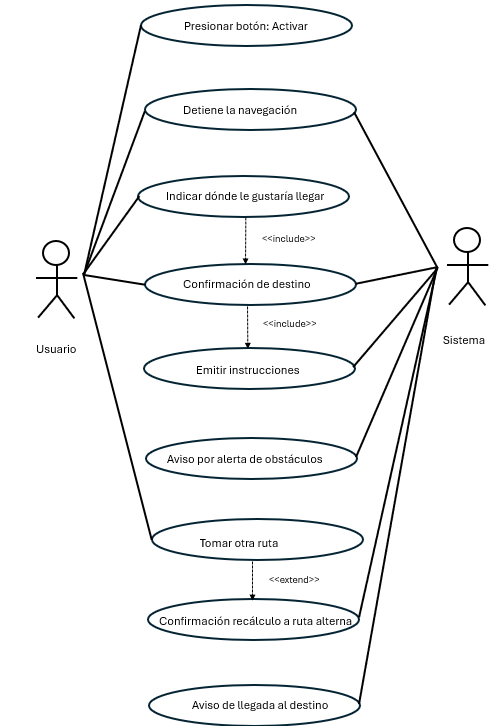
\includegraphics[width=13cm]{Diagramas/DiagCasoUso.png}
    \caption{Diagrama de casos de uso del sistema de navegación asistida}
    \label{fig:casos_uso}
\end{figure}

Este modelo permite identificar de forma clara las funcionalidades del sistema, así como las dependencias y comportamientos alternativos que pueden surgir durante su operación.
\\
El actor principal es el Usuario, quien interactúa directamente con el sistema mediante distintas funcionalidades. Por su parte, el Sistema actúa como el ente que procesa la información, toma decisiones y proporciona retroalimentación.

El usuario tiene la capacidad de activar el sistema “Presionar botón: Activar”. Este caso de uso representa la acción inicial que habilita la interacción con el sistema. Asimismo, el usuario puede detener la navegación en cualquier momento a través del caso de uso “Detiene la navegación”, lo que evidencia que el sistema debe permitir el control total sobre su ejecución.

“Indicar dónde le gustaría llegar”, donde el usuario proporciona el destino deseado. Este caso de uso describe una interacción directa en la que el sistema debe ser capaz de recibir y procesar la entrada del usuario. Asociado a este, se encuentra el caso de uso “Confirmación de destino”, el cual corresponde a una responsabilidad del sistema: validar y confirmar la información recibida. La relación <<include>> entre ambos indica que la confirmación es un comportamiento obligatorio que forma parte del servicio principal de captura de destino.

Una vez que el destino ha sido definido, el sistema ofrece la funcionalidad de “Emitir instrucciones”, que consiste en proporcionar indicaciones al usuario para llegar a su destino. Este caso de uso también está relacionado mediante <<include>>, lo que indica que depende de la confirmación previa del destino para ejecutarse correctamente.

Durante la interacción, el sistema incluye la capacidad de “Aviso por alerta de obstáculos”, lo cual representa una funcionalidad autónoma del sistema orientada a la seguridad del usuario. En este caso, el usuario no necesariamente inicia la acción, sino que el sistema actúa de manera proactiva notificando eventos relevantes del entorno.

“Tomar otra ruta”, está asociado a una relación <<extend>> con “Confirmación recálculo a ruta alterna”. Esta relación indica que se trata de una funcionalidad opcional que solo se activa bajo ciertas condiciones, como la detección de obstáculos o cambios en el entorno. En este contexto, el sistema asume la responsabilidad de recalcular una nueva ruta, mientras que el usuario participa de forma indirecta al recibir la confirmación de dicho ajuste.

El caso de uso “Aviso de llegada al destino”, representa la notificación al usuario de que se ha cumplido el objetivo de la navegación. Este caso de uso corresponde completamente al sistema, quien debe identificar el cumplimiento de la meta y comunicarlo oportunamente.

\section{Diagramas de flujo}
Con el objetivo de representar de manera detallada la secuencia operativa interna de este sistema, se emplea un diagrama de flujo, el cual describe los procesos, decisiones y ciclos que se ejecutan desde la activación del sistema hasta la llegada al destino.

\begin{figure}[H]
    \centering
    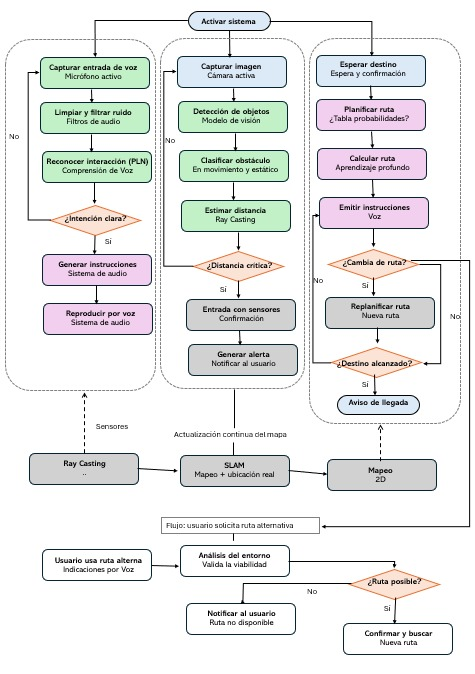
\includegraphics[width=13cm]{DiagFlujo/FlujoGeneral.jpeg}
    \caption{Diagrama de flujo global del sistema}
    \label{fig:flujo_gen}
\end{figure}
\textbf{Módulo 1 - Voz}
El sistema comienza capturando la entrada del usuario mediante el bloque “Capturar entrada de voz”, donde se utiliza el micrófono para recibir comandos. Posteriormente, la señal pasa por el proceso de “Limpiar y filtrar ruido”, en el cual se aplican técnicas de procesamiento de audio para mejorar la calidad de la señal.
\\
Una vez depurada, la información es interpretada en “Reconocer interacción (PLN)”, donde se emplean modelos de procesamiento de lenguaje natural para comprender la intención del usuario.
\\
Se presenta una decisión clave: “¿Intención clara?”.
\\
Si la respuesta es afirmativa, el sistema procede a “Generar instrucciones” y posteriormente a “Reproducir por voz”, proporcionando retroalimentación auditiva al usuario.
En caso contrario, el sistema puede requerir nueva entrada o repetir el proceso de interpretación.
\\
Este módulo es fundamental, ya que permite una interacción natural y accesible entre el usuario y el sistema.

\textbf{Módulo 2 - Visión}
\\
De manera paralela, el sistema activa la cámara en el bloque “Capturar imagen”, obteniendo información visual del entorno. Esta información es procesada en “Detección de objetos”, donde un modelo de visión identifica elementos relevantes.
\\
Posteriormente, en “Clasificar obstáculo”, el sistema determina si los objetos detectados representan un riesgo, diferenciando entre obstáculos móviles y estáticos.
\\
El siguiente paso es “Estimar distancia”, donde se calcula la proximidad de los objetos mediante técnicas como Ray Casting.
\\
Esto conduce a la decisión “¿Distancia crítica?”:
\\
Si se detecta un riesgo cercano, el sistema ejecuta “Entrada con sensores” para validar la información y posteriormente “Generar alerta”, notificando al usuario.
Si no existe riesgo, el sistema continúa monitoreando el entorno sin interrumpir la navegación.
\\
Este módulo garantiza la seguridad del usuario mediante análisis en tiempo real del entorno.

\textbf{Módulo 3 - Ruta}
En este módulo, el sistema puede encontrarse inicialmente en el estado “Esperar destino”, hasta recibir la confirmación del usuario. Una vez definido, se ejecuta “Planificar ruta”, donde se evalúan posibles trayectorias.
\\
Posteriormente, en “Calcular ruta”, se emplean algoritmos de aprendizaje profundo para determinar la mejor opción disponible. El resultado se comunica mediante “Emitir instrucciones”, guiando al usuario durante su desplazamiento.
\\
Durante la navegación, el sistema evalúa continuamente la condición “¿Cambia de ruta?”:
\\
Si no hay cambios, el sistema sigue emitiendo instrucciones.
Si ocurre un evento (por ejemplo, un obstáculo), se activa “Replanificar ruta”, generando una nueva trayectoria.
\\
Finalmente, se evalúa “¿Destino alcanzado?”:
\\
Si la respuesta es afirmativa, el sistema ejecuta “Aviso de llegada”, concluyendo el proceso.
En caso contrario, el ciclo de navegación continúa.

\textbf{Sensores y mapeo}
Se presenta:
SLAM (Mapeo y ubicación en tiempo real)
Mapeo 2D
Ray Casting
\\
Estos elementos permiten la actualización continua del entorno, proporcionando información clave a los módulos de visión y planificación. Gracias a este sistema, el modelo puede tomar decisiones informadas en tiempo real.
\\
Se contempla un flujo adicional cuando el usuario decide cambiar la ruta. Este proceso inicia en “Usuario usa ruta alterna”, seguido de un “Análisis del entorno” para validar la viabilidad.
\\
Se evalúa la decisión “¿Ruta posible?”:
\\
Si la ruta es viable, el sistema procede a “Confirmar y buscar nueva ruta”.
En caso contrario, se ejecuta “Notificar al usuario ruta no disponible”, informando la imposibilidad del cambio.
\subsection{Flujo de percepción}
Para los modulos que ayudan al sistema a percibir el mundo como el de Visión y el de los sensores, el flujo es:
El proceso interno del sistema para la detección, análisis y validación de obstáculos, integrando información proveniente de visión por computadora y sensores físicos. Su objetivo principal es garantizar que las decisiones de navegación se basen en información confiable, reduciendo falsos positivos y aumentando la seguridad del usuario.
\begin{figure}[H]
    \centering
    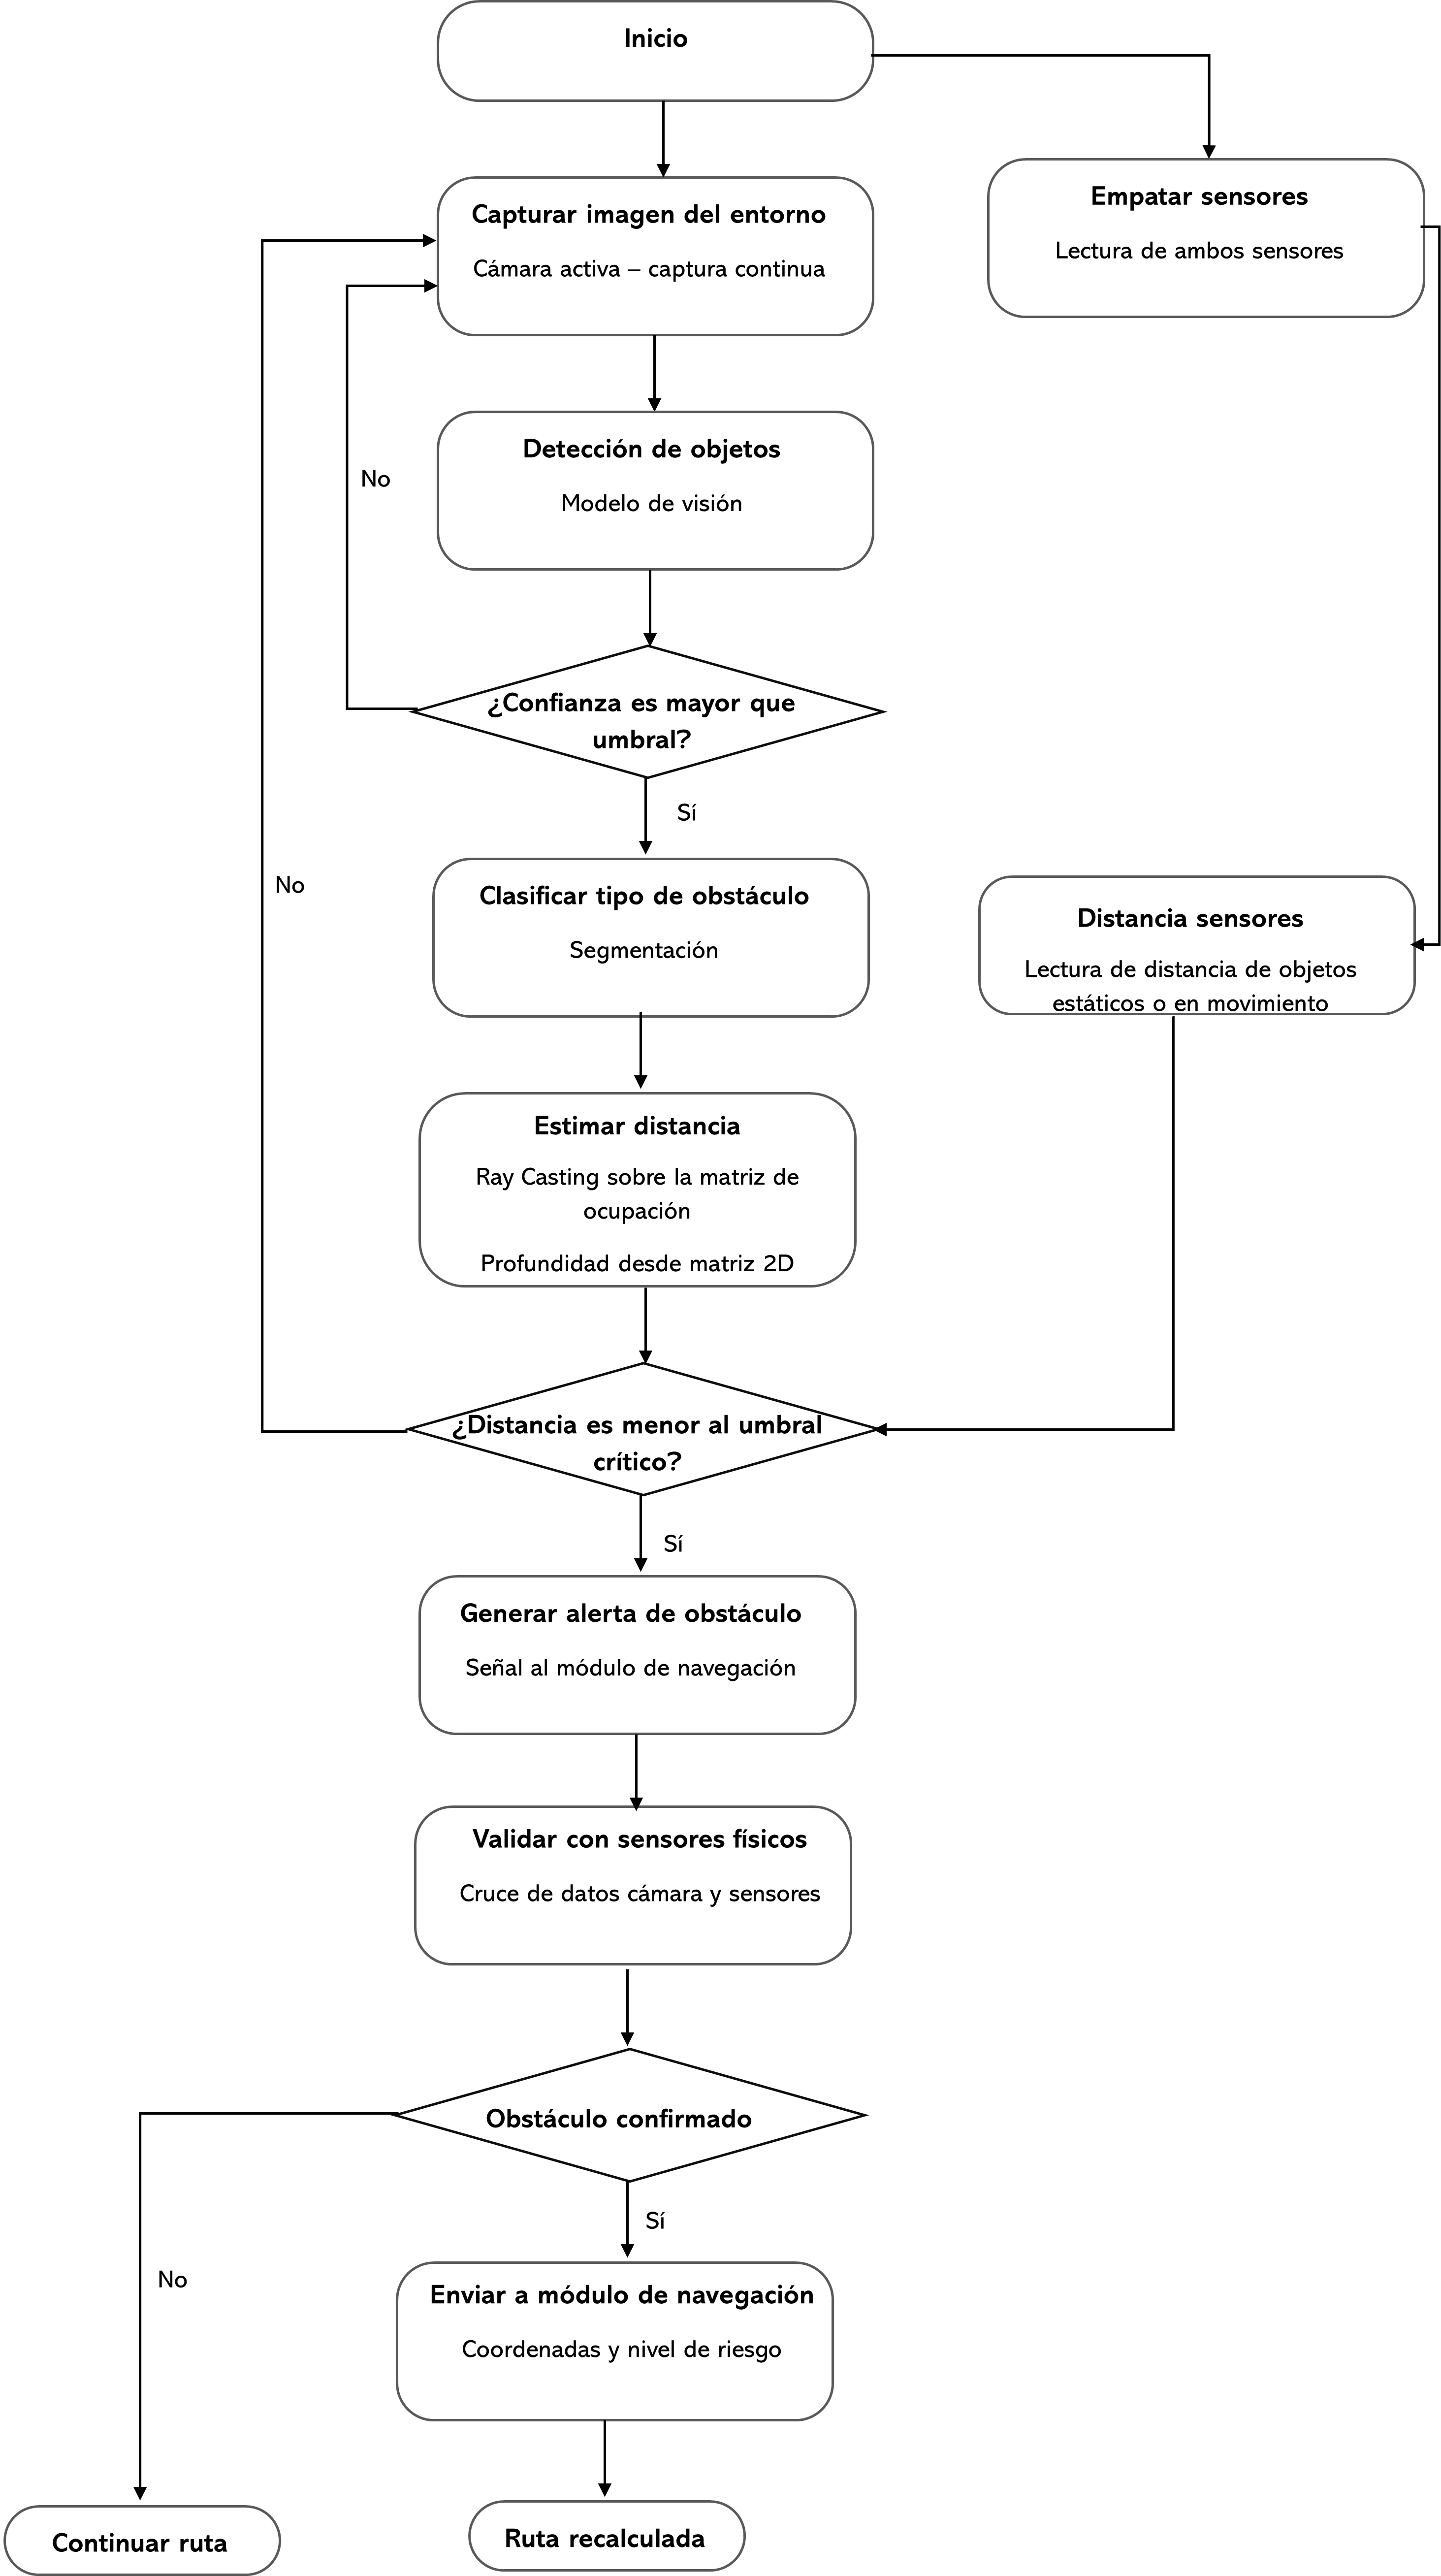
\includegraphics[width=11cm]{DiagFlujo/FlujoVision.png}
    \caption{Diagrama de flujo del Modulo de Vision y Modulo sensorial}
    \label{fig:flujo_vision}
\end{figure}
El flujo inicia a partir de dos procesos fundamentales:
Captura de imagen mediante una cámara activa y la entrada de los sensores, donde se realiza la lectura simultánea de los sensores físicos para sincronizar la información.

Una vez capturada la imagen, el sistema ejecuta el proceso de “Detección de objetos”, utilizando un modelo de visión por computadora para identificar elementos presentes en el entorno.

Posteriormente, se evalúa la condición “¿Confianza es mayor que umbral?”, la cual determina si la detección es suficientemente confiable:
Si la confianza no supera el umbral, el sistema descarta la detección y regresa al proceso de captura.
Si la confianza es adecuada, el flujo continúa con el análisis del objeto detectado.

Cuando la detección es válida, el sistema procede a “Clasificar tipo de obstáculo”, diferenciando entre objetos estáticos y dinámicos mediante técnicas de segmentación.
“Estimar distancia”, utiliza Ray Casting  sobre los objetos.

Los sensores físicos aportan información mediante el bloque “Distancia sensores”, proporcionando una medición adicional independiente de la visión.
Con la información obtenida, se evalúa la condición “¿Distancia es menor al umbral crítico?”:
Si no se encuentra dentro de un rango de riesgo, el sistema continúa monitoreando sin generar intervención.
Si la distancia es crítica, se activa el proceso de respuesta.

En este caso, el sistema ejecuta “Generar alerta de obstáculo”, enviando una señal al módulo de navegación para advertir la presencia de un posible riesgo.

“Validar con sensores físicos”, donde se cruzan los datos obtenidos por la cámara y los sensores.
A continuación, se evalúa la decisión “Obstáculo confirmado”:
Si no se confirma, el sistema descarta la alerta y continúa con la navegación normal.

Una vez validado el obstáculo se ejecuta “Enviar a módulo de navegación”, proporcionando las coordenadas del obstáculo y nivel de riesgo.

Con esta información, el sistema de navegación puede tomar decisiones informadas, como ajustar la trayectoria y recalcular la ruta.

Esto se refleja en el resultado “Ruta recalculada”. En caso de que no se confirme el obstáculo, el flujo concluye en “Continuar ruta”, manteniendo la trayectoria actual.

\subsection{Flujo de Navegación}
En este diagrama se explica el flujo de la navegación que se llevará a cabo.

\begin{figure}[H]
    \centering
    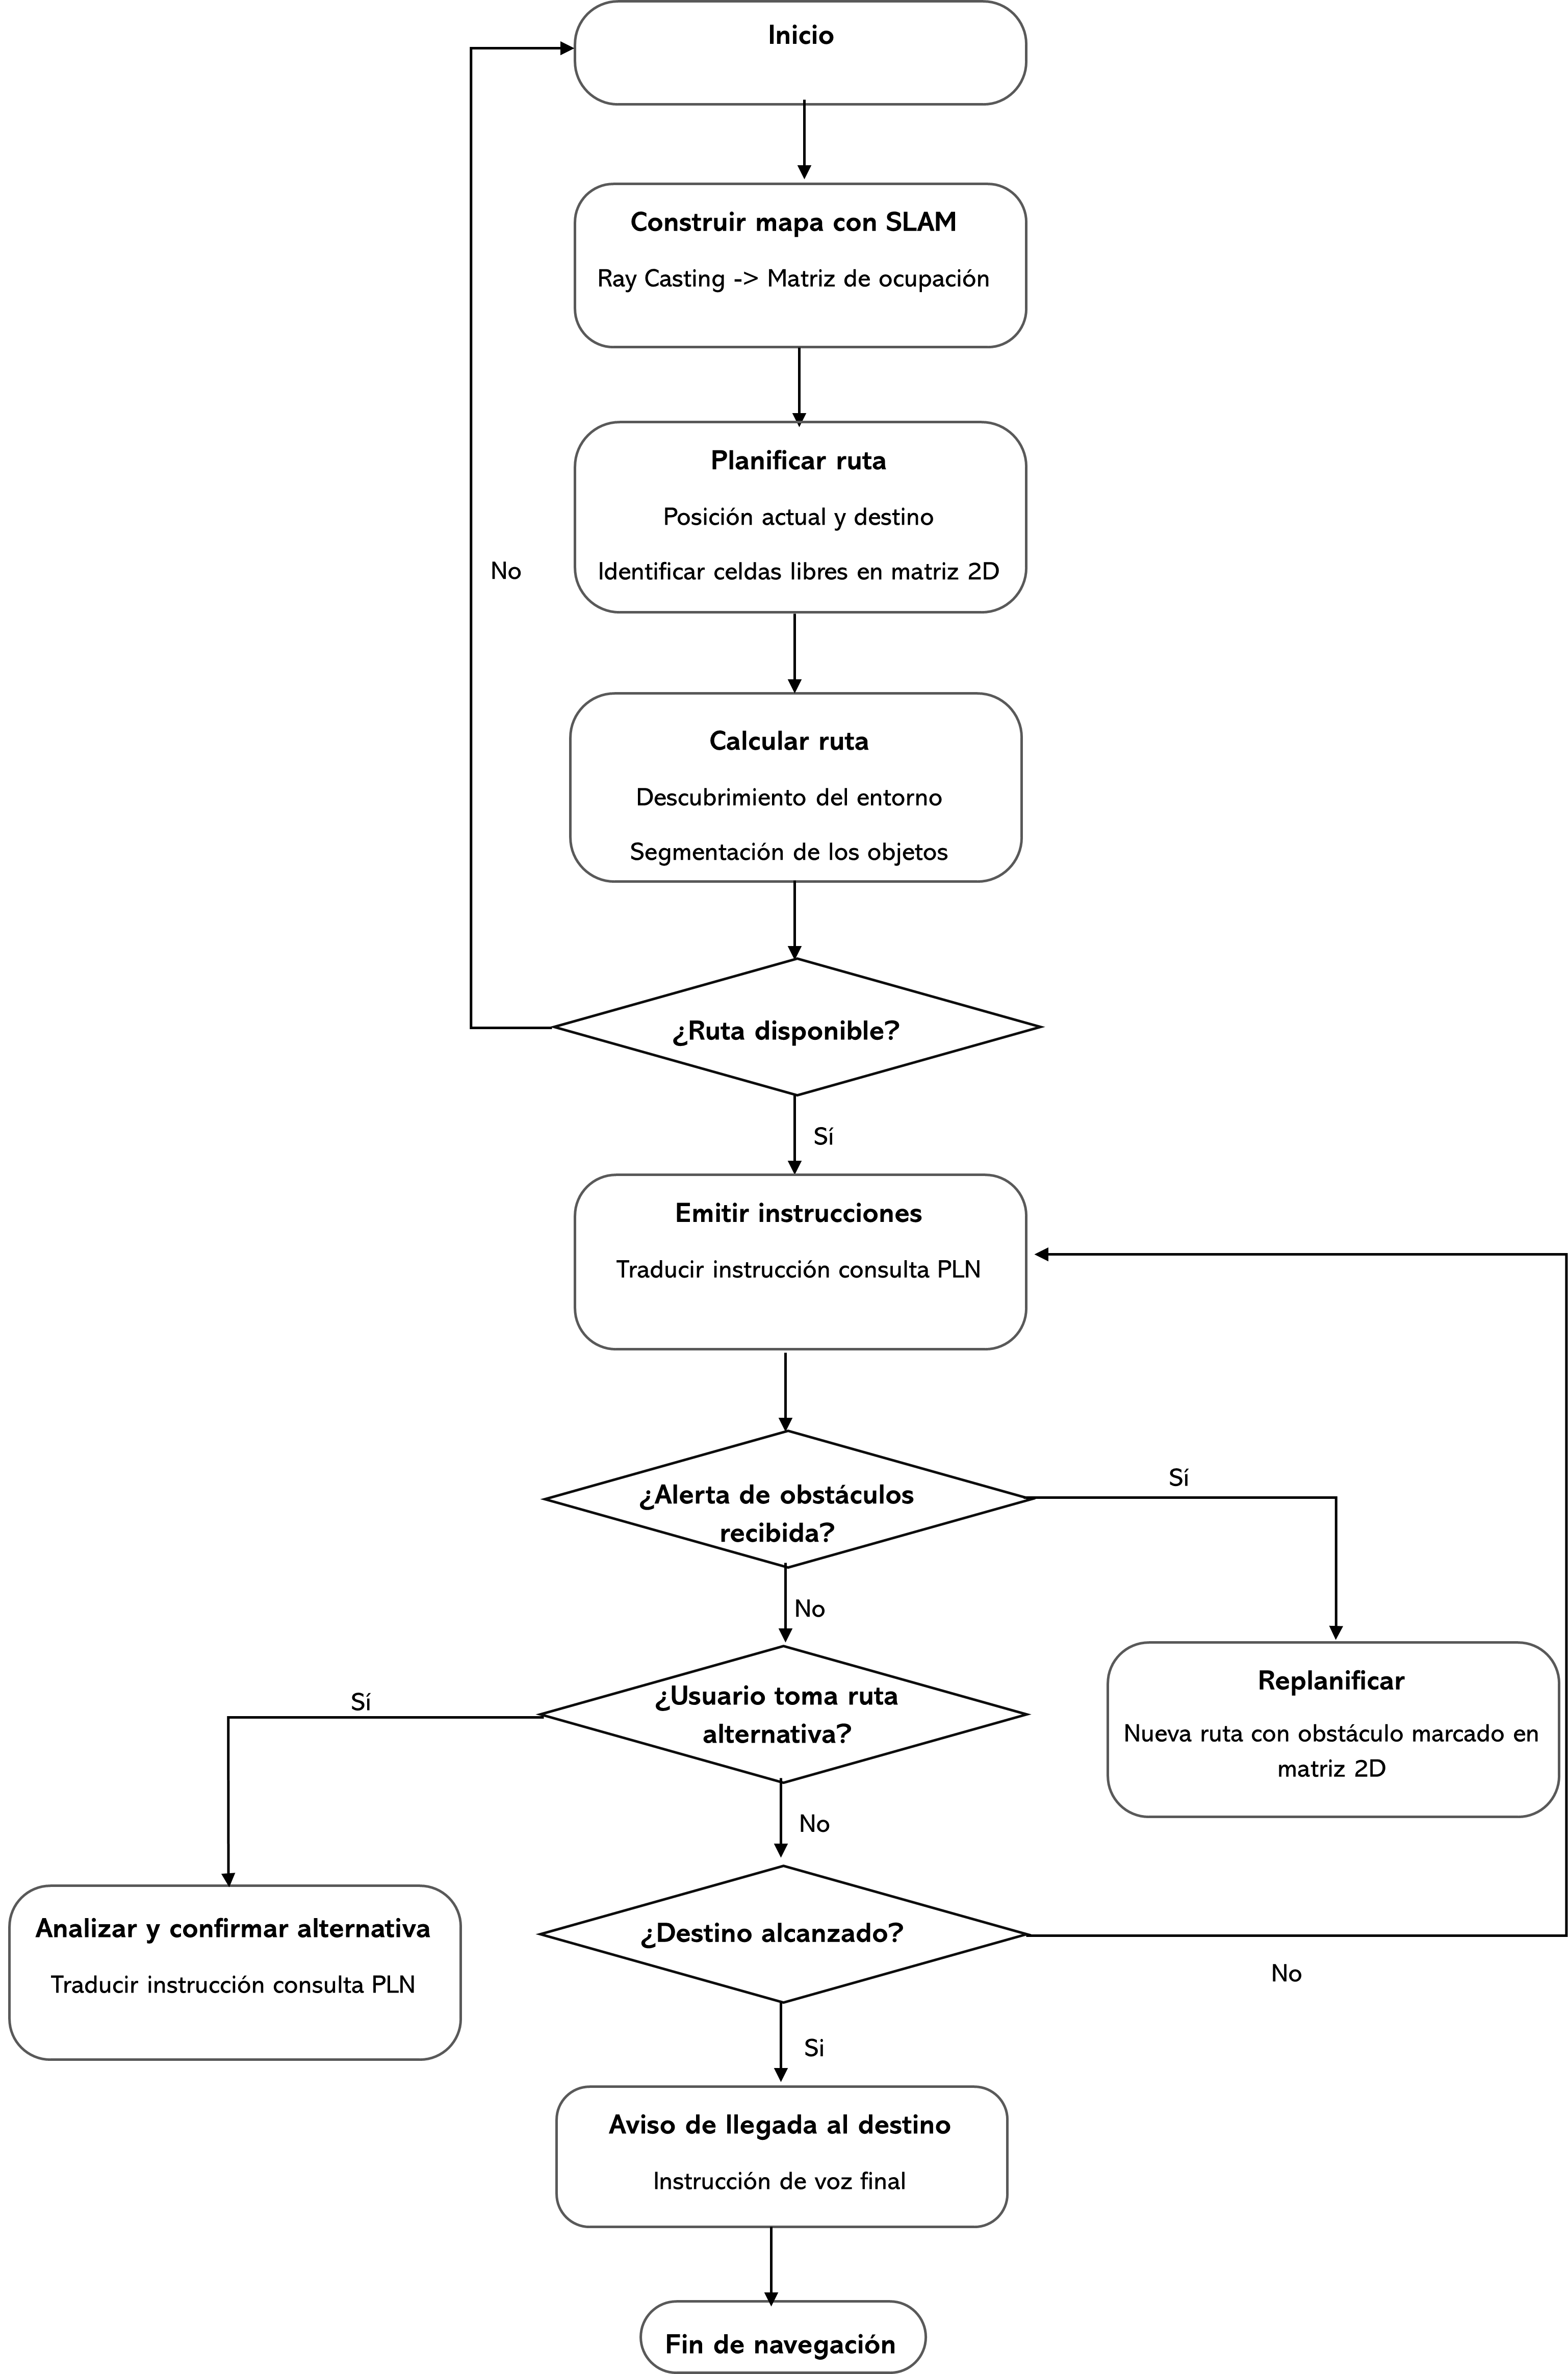
\includegraphics[width=11cm]{DiagFlujo/FlujoNavegacion.png}
    \caption{Diagrama de flujo del Modulo de Visión y Modulo sensorial}
    \label{fig:flujo_nav}
\end{figure}
El flujo inicia en el bloque Inicio y avanza hacia la construcción del entorno espacial mediante SLAM (Simultaneous Localization and Mapping), donde el sistema aplica Ray Casting para generar una matriz de ocupación 2D.

Con el mapa listo, el sistema ejecuta la planificación de ruta, identificando la posición actual, el destino y las celdas libres en la cuadrícula. 

A partir de esto, calcula la ruta mediante descubrimiento del entorno y segmentación de objetos. Si no existe una ruta disponible, el flujo regresa a planificar nuevamente. Cuando sí hay una ruta, se evalúa la condición ¿Ruta disponible? y el sistema procede a emitir instrucciones traducidas mediante procesamiento de lenguaje natural (PLN).

Desde ese punto se abre un ciclo de navegación activa:
Si llega una alerta de obstáculo, el sistema pasa a Replanificar, marcando el obstáculo en la matriz 2D y generando una nueva ruta, para luego volver a emitir instrucciones.

Si no hay alerta pero el usuario toma una ruta alternativa, el sistema la analiza y confirma mediante PLN.

Si no hay alerta y el usuario sigue la ruta, se evalúa si el destino fue alcanzado: si no, el ciclo regresa a emitir instrucciones; si sí, se emite un aviso de llegada por voz y el flujo concluye en Fin de navegación.

\subsection{Flujo de la Interacción}
Aquí se muestra como se comporta el flujo de los módulos de Reconocimiento de Voz, PLN y salida al usuario, permitiendo la interacción natural entre el usuario y el sistema de navegación asistida.

\begin{figure}[H]
    \centering
    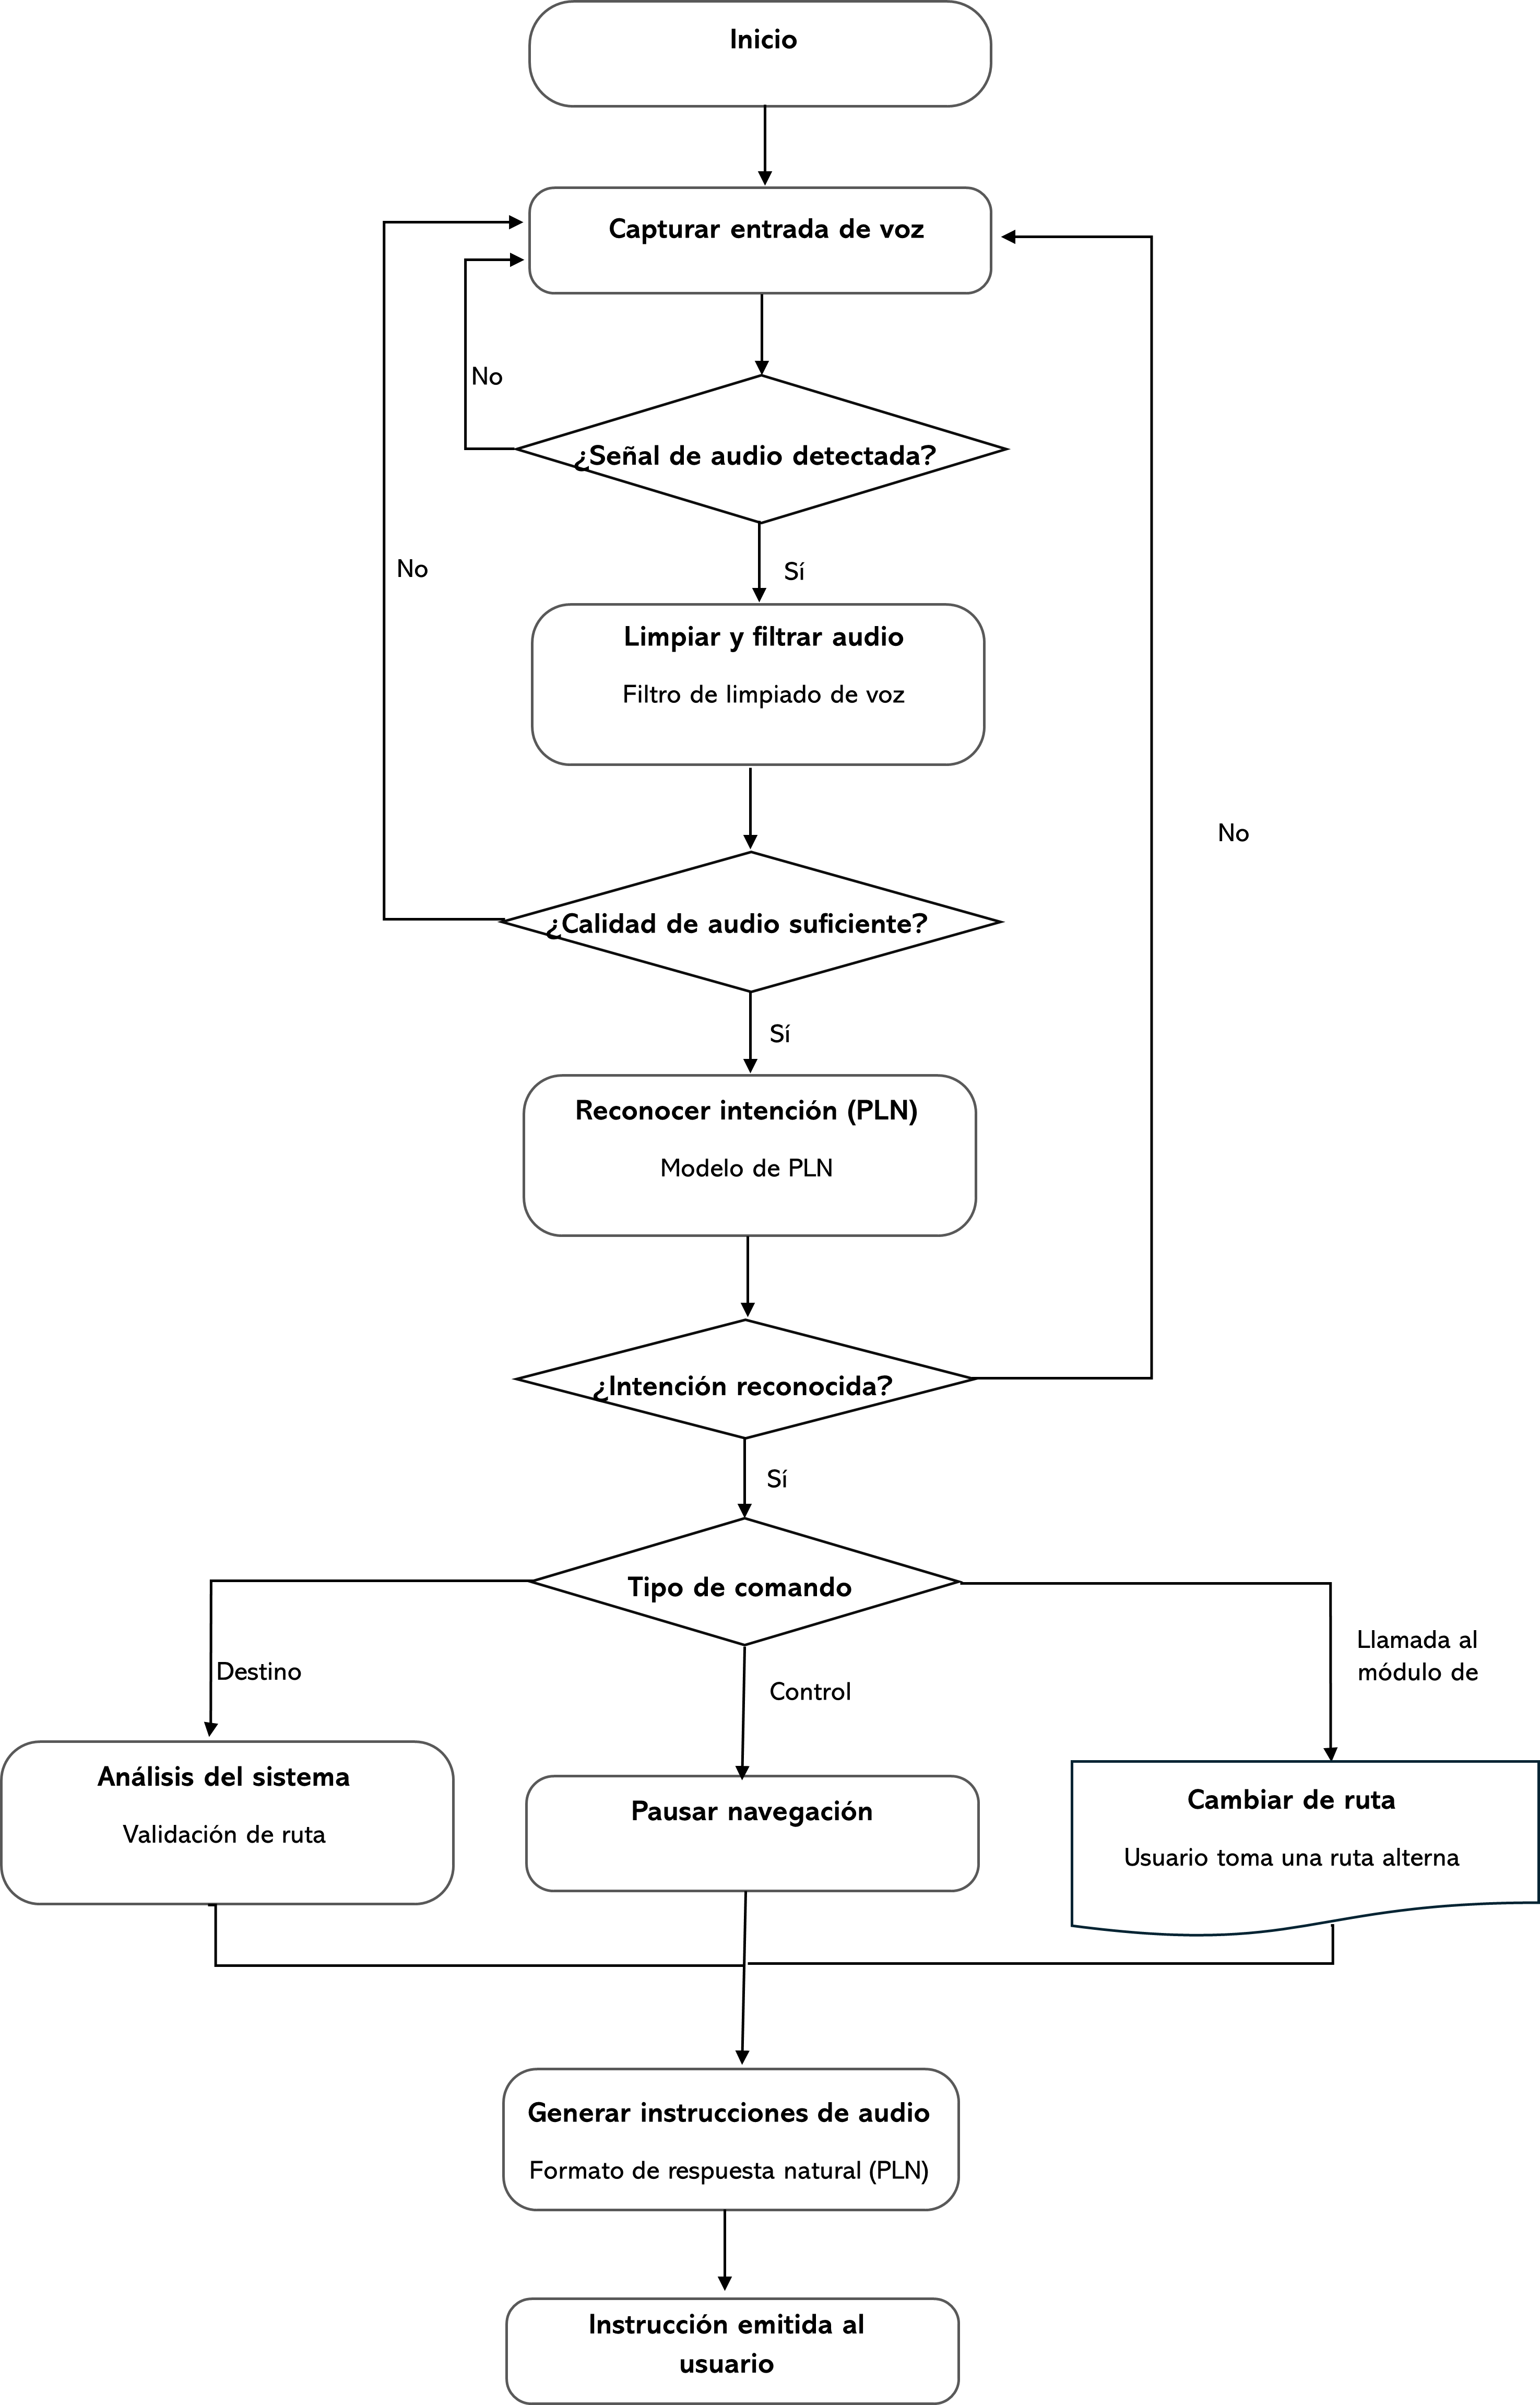
\includegraphics[width=11cm]{DiagFlujo/FlujoVozPLN.png}
    \caption{Diagrama de flujo del Modulo de Lenguaje Natural y Reconocimiento de voz}
    \label{fig:flujo_pln}
\end{figure}
El proceso inicia en el bloque “Inicio”, seguido de “Capturar entrada de voz”, donde el sistema activa el micrófono para adquirir señales de audio de manera continua.
Se evalúa la condición “¿Señal de audio detectada?”:
Si no se detecta señal, el sistema permanece en estado de espera y continúa monitoreando la entrada de audio.
Si se detecta señal, el flujo avanza al procesamiento de la misma.

Una vez detectada la señal, el sistema ejecuta el bloque “Limpiar y filtrar audio”, donde se aplican técnicas de reducción de ruido y mejora de calidad.
Se evalúa “¿Calidad de audio suficiente?”:
Si la calidad no es adecuada, el sistema descarta la señal y regresa a la captura, evitando interpretaciones erróneas.
Si la calidad es suficiente, el flujo continúa hacia el análisis semántico.
Este paso es fundamental para garantizar la confiabilidad del reconocimiento.

El sistema procesa la señal mediante el bloque “Reconocer intención (PLN)”, utilizando un modelo de procesamiento de lenguaje natural para interpretar el contenido del mensaje y se evalúa la condición “¿Intención reconocida?”:
Si no se reconoce la intención, el sistema vuelve al estado de captura, solicitando implícitamente una nueva entrada.
Si la intención es reconocida, el flujo continúa hacia la clasificación del comando.

Una vez comprendida la intención, el sistema clasifica la solicitud en el bloque “Tipo de comando”, distinguiendo tres puntos principales:
\begin{enumerate}
    \item Comandos de destino: Se dirigen al bloque “Análisis del sistema”, donde se realiza la validación de la ruta hacia el destino solicitado. Este proceso implica verificar la viabilidad del trayecto y preparar la navegación.
    \item Comandos de control: Incluyen acciones como “Pausar navegación”, permitiendo al usuario modificar el estado del sistema en tiempo real.
    \item Cambio de ruta: Corresponde al bloque “Cambiar de ruta”, donde el usuario solicita una alternativa. Este caso implica la comunicación con el módulo de navegación para recalcular el trayecto.
\end{enumerate}
Independientemente del tipo de comando, el sistema procede al bloque “Generar instrucciones de audio”, donde se construye una respuesta en lenguaje natural mediante técnicas de PLN.

Finalmente, se ejecuta “Instrucción emitida al usuario”, proporcionando retroalimentación auditiva clara y comprensible.

\section{Arquitectura}

A continuación se describe la arquitectura del sistema propuesto, la cual define los módulos que lo componen, su función dentro del flujo de procesamiento y la manera en que interactúan entre sí para lograr una navegación asistida coherente y en tiempo real.

\subsection{Diagrama de arquitectura}

El siguiente diagrama presenta la arquitectura modular del sistema de navegación asistida, mostrando cómo interactúan sus tres fuentes de entrada principales: la voz del usuario, la cámara y los sensores físicos. 

\begin{figure}[H]
    \centering
    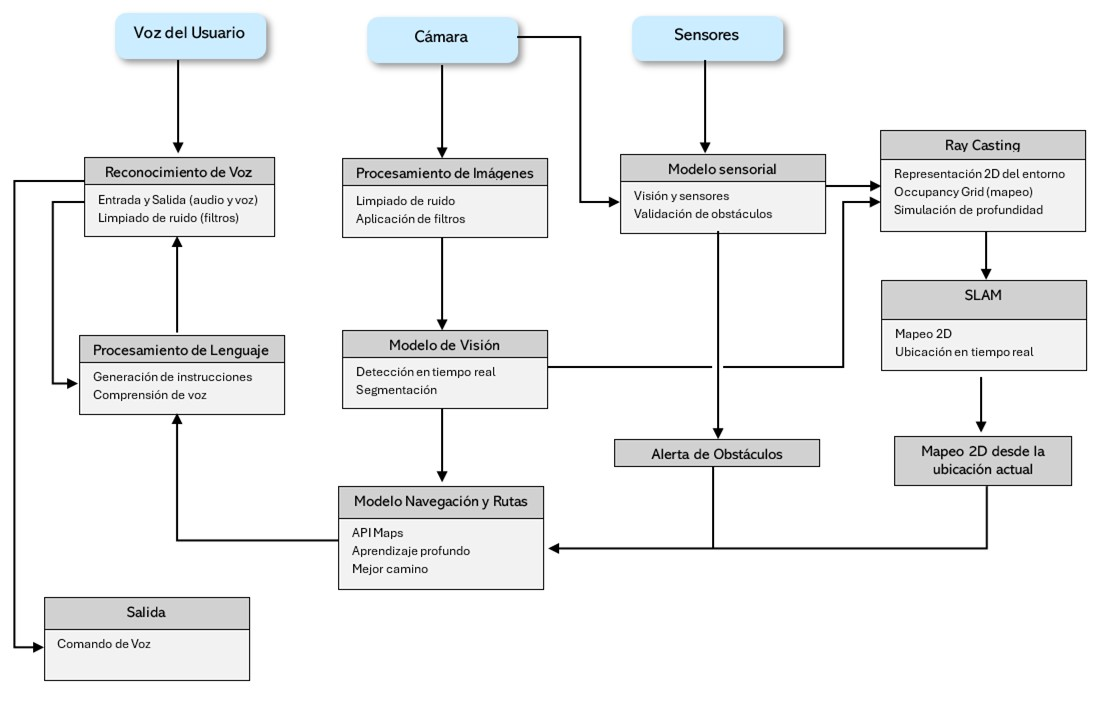
\includegraphics[width=17cm]{Diagramas/DiagArquitectura2.jpg}
    \caption{Diagrama de arquitectura general del sistema}
    \label{fig:arquitectura}
\end{figure}
El sistema tiene tres entradas principales: voz, cámara y sensores. La cámara pasa por procesamiento de imagen y luego por el modelo de visión, cuya tarea clave es la segmentación: detectar objetos y extraer sus coordenadas en el espacio (básicamente "hay un obstáculo en X, Y"). Esas coordenadas son una de las dos entradas más importantes al módulo de navegación.
\\
La entrada dada por el mapeo es resultante de la cadena generada por SLAM donde se obtiene un mapa en 2D con ubicación actual, el flujo se basa en los sensores y el Ray Casting que construye un Occupancy Grid, es decir, una rejilla que indica las celdas libres y ocupadas. Esa matriz 2D es literalmente el terreno sobre el que se calcula la ruta.
\\
El módulo de navegación y rutas recibe 3 entradas:
\begin{itemize}
    \item La matriz 2D con el mapa del entorno
    \item  Las coordenadas de objetos que detectó el modelo de visión (la segmentación)
    \item  Múltiples rutas basadas en la probabilidad de pesos que le asignan costo o preferencia a distintos caminos, así el sistema no solo busca el camino más corto geométricamente sino el más probable o seguro según la posibilidad de caminos que ha evaluado previamente el modelo.
\end{itemize}
Con esas tres entradas se calcula la mejor ruta.


Los sensores son alarmas en las que si detectan un obstáculo inesperado, generan una alerta que va directo al módulo de navegación para forzar un recalculado de la ruta, esto con el fin de evitar obstáculos. Esto es independiente del flujo normal, es una interrupción reactiva.
\\
La salida es dada con la ruta calculada, el sistema extrae las instrucciones paso a paso y las va entregando como salida de voz en tiempo real apoyado en la salida dada por el procesamiento de lenguaje que representa el sistema, también actualiza su estado interno conforme avanza, para dar las instrucciones adecuadas.

\section{Análisis de Requerimientos}

El presente capítulo tiene como objetivo establecer el puente entre los requerimientos
definidos en el capítulo anterior y las decisiones tecnológicas que dan forma a la
implementación del sistema. Cada tecnología elegida responde a uno o más requerimientos
concretos y se justifica con base en los fundamentos teóricos estudiados en el marco
teórico. El análisis se organiza por agrupación de módulos, siguiendo la misma
estructura arquitectónica del sistema.

Es importante señalar que la selección no se basa únicamente en la capacidad funcional
de cada tecnología, sino también en su viabilidad dentro de las restricciones
establecidas por los requerimientos no funcionales: operación en hardware embebido
de recursos limitados (RNF-05), operación autónoma sin conexión a internet (RNF-13)
y latencias de respuesta acotadas (RNF-01, RNF-02).

% ===
\subsection{Módulos de percepción}
% ======

Los módulos de percepción son el punto de entrada de toda la información que el sistema
procesa. Su función es transformar señales físicas ---fotogramas de cámara y lecturas
de sensores--- en representaciones computacionales útiles para los módulos posteriores.
Los requerimientos que gobiernan esta capa son especialmente exigentes en términos de
latencia (RNF-01), precisión (RNF-06) y eficiencia computacional (RNF-05), lo que
reduce significativamente el espacio de opciones tecnológicas viables.

\subsubsection{Preprocesamiento de imágenes: OpenCV y NumPy}

El requerimiento RF-07 establece que el sistema debe adquirir fotogramas de forma
continua y aplicar operaciones de preprocesamiento antes de alimentar el módulo de
visión. Según la literatura, el preprocesamiento transforma los datos visuales sin
procesar en un formato adecuado para el análisis posterior, eliminando distorsiones y
resaltando las características relevantes \cite{unitxlabs_prepost}. Operaciones como
redimensionamiento, normalización e igualación de contraste son necesarias porque un
modelo de detección produce resultados más estables cuando recibe entradas homogéneas,
reduciendo la variabilidad innecesaria debida a condiciones de iluminación o escala.

Para esta etapa se elige \textbf{OpenCV} (\texttt{cv2}) en combinación con
\textbf{NumPy}. OpenCV es una biblioteca de código abierto especializada en visión por
computadora que implementa de forma eficiente las operaciones de preprocesamiento
requeridas, y NumPy proporciona la estructura de datos matricial sobre la que se
representan las imágenes como arreglos numéricos. Ambas bibliotecas están ampliamente
documentadas, tienen una implementación madura y pueden ejecutarse sin aceleración GPU,
lo cual es indispensable dado que el hardware objetivo es una plataforma embebida
(RNF-05). Además, al operar localmente sin dependencia de servicios externos, se
garantiza el cumplimiento de RNF-13.

\subsubsection{Detección de objetos: YOLOv8}

El requerimiento central de los módulos de percepción es RF-08, que exige detectar
objetos relevantes para la navegación en cada fotograma con su localización espacial y
nivel de confianza. Este requerimiento se complementa con RF-09, que requiere asignar
a cada objeto una categoría semántica y un nivel de riesgo. Dado que el ciclo completo
desde la captura hasta la alerta no debe superar los 300~ms (RNF-01) y que la tasa de
detección correcta debe ser de al menos el 90\% (RNF-06), se necesita un modelo que
combine velocidad y precisión.

Como se estudió en el marco teórico, los detectores de una sola etapa como YOLO realizan
la extracción de características y la predicción de objetos en un único paso, lo que les
permite procesar imágenes con mayor velocidad que los detectores de dos etapas como
Faster R-CNN \cite{geeksforgeeks_object_detection}. YOLO divide la imagen en una
cuadrícula y predice simultáneamente las cajas delimitadoras y las clases presentes en
cada región \cite{geeksforgeeks_object_detection}, lo que lo convierte en la arquitectura
más adecuada para una aplicación con restricciones de latencia en tiempo real.

Se elige específicamente \textbf{YOLOv8} en su implementación de \textbf{Ultralytics},
ya que esta versión introduce mejoras arquitectónicas respecto a versiones anteriores,
mantiene compatibilidad con exportación en formato ONNX para optimización en plataformas
embebidas, y ofrece una API de uso directo en Python que simplifica la integración.
Además, su entrenamiento puede realizarse sobre conjuntos de datos especializados en
objetos relevantes para la navegación peatonal, lo que permite ajustar el modelo a los
casos de uso específicos del sistema (personas, puertas, escaleras, obstáculos estáticos).

\subsubsection{Detección de proximidad: sensores ultrasónicos}

El requerimiento RF-10 exige estimar la distancia entre el usuario y los objetos
detectados, y el requerimiento RF-11 establece que esta estimación debe validarse con
mediciones de sensores físicos para reducir falsas alarmas. La validación cruzada entre
visión y sensores tiene especial relevancia en situaciones donde la iluminación es baja
o cuando un objeto no se captura con suficiente claridad en la cámara.

Como se expone en el marco teórico, los sensores ultrasónicos miden distancias mediante
el tiempo de vuelo de un pulso sonoro y ofrecen una lectura sencilla y económica para
cortas y medias distancias \cite{hcsr04_datasheet}. Si bien los sensores ToF ofrecen
mayor precisión y menor tamaño \cite{vl53l1x_product}, los sensores ultrasónicos como
el HC-SR04 resultan suficientes para validar la presencia o ausencia de obstáculos
cercanos dentro de un rango de operación de 2~cm a 4~m \cite{hcsr04_datasheet}, que
cubre los casos críticos de navegación peatonal. Su implementación mediante el protocolo
I2C sobre la plataforma embebida es directa mediante bibliotecas como \texttt{smbus2}
o \texttt{RPi.GPIO}, sin requerir hardware adicional ni procesamiento significativo.

\subsubsection{Inferencia contextual y fusión sensorial}

El requerimiento RF-13 exige que el sistema infiera relaciones contextuales entre
objetos detectados, como el estado de apertura de una puerta o el grado de obstrucción
de un pasillo, para enriquecer la representación del entorno más allá de la detección
individual. El requerimiento RF-12 establece que el sistema solo debe emitir una alerta
al \emph{confirmar} un obstáculo, no al simplemente detectarlo, lo cual requiere un
mecanismo de validación probabilística.

Para esta función se adopta un modelo de \textbf{inferencia probabilística basada en
reglas}, implementado en Python. Este enfoque corresponde
al aprendizaje supervisado descrito en el marco teórico, donde la inferencia probabilística es la base para clasificación \cite{ibm2025_mltypes}. La elección de
un modelo probabilístico ligero, en lugar de una red neuronal compleja, responde
directamente a RNF-05: la inferencia contextual debe ejecutarse en hardware embebido
de recursos limitados sin introducir latencia adicional significativa al ciclo de
percepción. La fusión de la salida del módulo de visión con la lectura de sensores
se realiza mediante umbrales de confianza configurables, garantizando el comportamiento
conservador requerido por RNF-09.

% =====
\subsection{Módulos de representación}
% =======
Los módulos de representación transforman la información perceptual en una estructura
espacial que el módulo de navegación puede utilizar para planificar rutas. El mapa
generado debe distinguir zonas libres de zonas ocupadas (RF-16), actualizarse a una
frecuencia mínima de 10~Hz (RNF-03) y construirse de forma incremental sin necesidad
de un mapa previo (RF-15).

\subsubsection{Representación del entorno: occupancy grid con NumPy}

Como se estudió en el marco teórico, los mapas de ocupación representan el entorno
mediante una cuadrícula de celdas donde cada celda almacena la probabilidad de estar
ocupada por un obstáculo \cite{elfes1989}. Este concepto introducido por Elfes en 1989
es uno de los métodos más utilizados en robótica móvil para representar entornos
desconocidos, ya que cada celda puede clasificarse como libre, ocupada o desconocida
\cite{elfes1989}, lo cual corresponde exactamente a la representación requerida por
RF-16.

La \textit{occupancy grid} se implementa como una matriz bidimensional gestionada con
\textbf{NumPy}, aprovechando sus operaciones vectorizadas para actualizar múltiples
celdas en un solo paso. Esta elección garantiza eficiencia computacional (RNF-05) y
evita la necesidad de dependencias externas para el manejo matricial. La representación
en formato \textit{log-odds} permite actualizar probabilidades de ocupación de forma
incremental y numéricamente estable, acumulando observaciones a lo largo del tiempo.

\subsubsection{Estimación de posición: SLAM simplificado con EKF}

El requerimiento RF-14 exige mantener una estimación continua de la posición y
orientación del usuario integrando movimiento y percepción, y el requerimiento RF-15
añade que esta estimación debe construirse de forma incremental sin mapa previo. Estos
dos requerimientos describen conjuntamente el problema clásico de \textit{Simultaneous
Localization and Mapping} (SLAM), cuyo objetivo es estimar simultáneamente la pose del
agente y el mapa del entorno a partir únicamente de sus propias observaciones
\cite{wikipedia_slam}.

Dado que el hardware objetivo es una plataforma embebida con recursos limitados
(RNF-05), una implementación completa de SLAM como ORB-SLAM o LiDAR-SLAM sería
inviable: estos sistemas requieren procesamiento intensivo de nubes de puntos o de
descriptores visuales que excede la capacidad de una Raspberry Pi 4 operando en tiempo
real. Por ello se opta por un \textbf{SLAM simplificado orientado a mapeo local},
apoyado en un \textbf{Filtro de Kalman Extendido} (EKF) implementado en Python con
NumPy. Esta elección equilibra la necesidad de localización continua (RF-14) con la
restricción de recursos (RNF-05).

\paragraph{Representación del estado.}
La pose del usuario se modela como un vector de estado tridimensional:
\[
\mathbf{x}_t = [x_t,\; y_t,\; \theta_t]^T
\]
donde $(x_t, y_t)$ es la posición en el plano 2D y $\theta_t$ es la orientación.
Esta representación es suficiente para el dominio de navegación peatonal en superficies
planas y evita la complejidad computacional de una pose en 6 grados de libertad.

\paragraph{Modelo de movimiento (etapa de predicción).}
En cada ciclo, la pose se propaga hacia adelante usando los incrementos de odometría
$(\Delta d,\, \Delta\theta)$ estimados a partir del desplazamiento del usuario:
\[
\mathbf{x}_t^{-} = \mathbf{x}_{t-1} +
\begin{bmatrix}
\Delta d \cos(\theta_{t-1}) \\
\Delta d \sin(\theta_{t-1}) \\
\Delta\theta
\end{bmatrix}
\]
Este modelo de movimiento unicycle es no lineal en $\theta$, lo que justifica el uso
del EKF en lugar del filtro de Kalman estándar: el EKF linealiza localmente las
funciones no lineales mediante jacobianos, haciendo manejable la propagación de
incertidumbre sin abandonar el marco probabilístico \cite{thrun2005probabilistic}.
La covarianza del estado se propaga como:
\[
\mathbf{P}_t^{-} = \mathbf{F}\,\mathbf{P}_{t-1}\,\mathbf{F}^T + \mathbf{Q}
\]
donde $\mathbf{F}$ es el jacobiano del modelo de movimiento respecto al estado y
$\mathbf{Q}$ es la covarianza del ruido de proceso, que modela la incertidumbre
acumulada por la odometría aproximada.\cite{thrun2005probabilistic}.

\paragraph{Corrección con mediciones (etapa de actualización).}
Una vez obtenida la predicción, el EKF la corrige con las mediciones reales
provenientes de los sensores de proximidad. La ganancia de Kalman $\mathbf{K}$
determina cuánto peso se otorga a la medición frente a la predicción:
\[
\mathbf{K} = \mathbf{P}_t^{-}\mathbf{H}^T
             \bigl(\mathbf{H}\mathbf{P}_t^{-}\mathbf{H}^T + \mathbf{R}\bigr)^{-1}
\]
La pose y la covarianza se actualizan a partir de la innovación, es decir, la
diferencia entre la medición real $\mathbf{z}_t$ y la medición esperada
$h(\mathbf{x}_t^{-})$ según el modelo de observación $h(\cdot)$:
\[
\mathbf{x}_t = \mathbf{x}_t^{-} + \mathbf{K}\bigl(\mathbf{z}_t - h(\mathbf{x}_t^{-})\bigr)
\]
\[
\mathbf{P}_t = (\mathbf{I} - \mathbf{K}\mathbf{H})\,\mathbf{P}_t^{-}
\]
donde $\mathbf{H}$ es el jacobiano de $h(\cdot)$ respecto al estado y $\mathbf{R}$ es
la covarianza del ruido de medición de los sensores. Cuando la innovación es pequeña
(la predicción coincide bien con la medición) $\mathbf{K}$ se acerca a cero y se
confía más en el modelo; cuando es grande, $\mathbf{K}$ crece y la medición tiene
mayor peso sobre la estimación final. Este mecanismo autorregulado es lo que hace al
EKF robusto ante la acumulación de error de odometría \cite{thrun2005probabilistic}.

\paragraph{Actualización del mapa en log-odds.}
En paralelo a la estimación de la pose, el mapa de ocupación se actualiza de forma
incremental usando una representación en log-odds. Cada celda $c$ almacena el
logaritmo de la razón de probabilidades de estar ocupada frente a estar libre:
\[
l_t(c) = l_{t-1}(c) +
\log\frac{p(\mathbf{z}_t \mid c = \text{occ})}{p(\mathbf{z}_t \mid c = \text{free})}
\]
Esta representación tiene dos ventajas directas que justifican su elección. Primero,
la actualización es aditiva e incremental: cada nueva medición simplemente suma un
término al valor acumulado de la celda, sin necesidad de recalcular probabilidades
completas. Segundo, trabajar en escala logarítmica evita problemas numéricos de
underflow cuando las probabilidades se acercan a cero o a uno tras muchas
observaciones, lo que es frecuente en celdas cercanas al usuario
\cite{thrun2005probabilistic}. Los valores de log-odds se saturan en un rango
$[l_{\min},\, l_{\max}]$ para limitar el tiempo que el sistema tarda en corregir
una celda marcada erróneamente, garantizando que el mapa siga siendo actualizable
ante cambios dinámicos del entorno (RF-17).

\subsubsection{Actualización del mapa: ray casting con algoritmo de Bresenham}

El requerimiento RF-17 establece que el mapa debe actualizarse en respuesta a cambios
detectados en el entorno, y RNF-03 fija una frecuencia mínima de 10~Hz para esta
actualización. El mecanismo de actualización debe ser computacionalmente ligero para
no comprometer la latencia global del sistema.

Como se explica en el marco teórico, el ray casting permite proyectar rayos desde la
posición estimada del usuario para actualizar las celdas del mapa: las celdas recorridas
por el rayo se marcan como libres y la celda donde el rayo se detiene se marca como
ocupada \cite{elfes1989}. Para recorrer las celdas de forma eficiente se utiliza el
\textbf{algoritmo de Bresenham} \cite{bresenham1965}, que permite identificar las celdas
atravesadas por un rayo mediante operaciones aritméticas simples, sin multiplicaciones
ni divisiones en punto flotante. Como se señala en el marco teórico, el ray casting
presenta un bajo costo computacional, puede ejecutarse en CPU sin necesidad de GPU y es
compatible con mapas discretos basados en cuadrículas \cite{stackoverflow_raycasting},
lo que lo convierte en la técnica más adecuada para cumplir RNF-03 y RNF-05
simultáneamente, a diferencia del ray tracing, que requiere procesamiento
significativamente mayor \cite{stackoverflow_raycasting}.

% ====
\subsection{Módulo de navegación y rutas}
% ======

El módulo de navegación es el núcleo decisional del sistema. Debe calcular rutas
óptimas sobre el mapa local (RF-18), actualizarlas periódicamente (RF-19),
recalcularlas de forma inmediata ante obstáculos confirmados (RF-20), traducirlas
en instrucciones de movimiento (RF-21), resolver destinos sobre el mapa del entorno
(RF-22) y gestionar la seguridad del usuario como prioridad (RNF-09).

\subsubsection{Navegación local: aprendizaje por refuerzo profundo (DRL)}

A diferencia de los algoritmos clásicos de búsqueda de caminos como A* o Dijkstra,
que requieren un mapa completamente conocido y estático para operar de forma óptima
\cite{hart1968astar, dijkstra1959}, la navegación en entornos peatonales reales implica
incertidumbre, cambios dinámicos y necesidad de adaptación continua. El requerimiento
RF-19 establece que la ruta se recalcula periódicamente durante la navegación, pero
RF-20 exige recálculo inmediato ante un obstáculo confirmado: esta combinación describe
un agente que debe tomar decisiones secuenciales bajo incertidumbre, que es exactamente
el dominio del aprendizaje por refuerzo.

Como se estudió en el marco teórico, el aprendizaje por refuerzo es un enfoque en el
que un agente aprende a tomar decisiones mediante la interacción con su entorno,
recibiendo recompensas o penalizaciones, con el objetivo de aprender una política que
maximice la recompensa acumulada \cite{ibm2025_mltypes}. Al combinarlo con redes
neuronales profundas, el agente es capaz de aprender representaciones complejas del
entorno directamente desde los datos de los sensores, lo que lo hace especialmente
adecuado para espacios de estado continuos y entornos con obstáculos dinámicos como
los que enfrenta el sistema \cite{ibm2025_mltypes}.

Se propone el uso de \textbf{aprendizaje por refuerzo profundo} (DRL) para la
navegación local, con un espacio de acciones discreto compuesto por las cuatro
decisiones posibles del sistema: avanzar, girar a la izquierda, girar a la derecha
y detenerse. El estado del entorno se representa como un vector compacto que incluye
las distancias al obstáculo más cercano en cada dirección, la posición relativa al
siguiente waypoint y los niveles de riesgo detectados por el módulo de percepción.
La selección específica del algoritmo de entrenamiento, el entorno de simulación y
la estrategia de transferencia al hardware real se definirán en la segunda etapa del
trabajo terminal, una vez validado el comportamiento del resto de los módulos del
sistema.

\subsubsection{Submódulo de dirección: traducción de acciones}

El requerimiento RF-21 exige que la acción elegida por el modelo se traduzca en una
instrucción discreta y comprensible para el usuario. Dado que el espacio de acciones
del modelo de RL es ya discreto (avanzar, girar izquierda, girar derecha, detenerse),
esta traducción puede implementarse mediante \textbf{reglas determinísticas simples}
en Python: cada índice de acción se mapea directamente a una instrucción de texto con
distancia y ángulo aproximados. La complejidad del sistema se concentra en el modelo de
decisión; la capa de traducción no requiere aprendizaje ni módulos adicionales. Esto
garantiza latencia baja y comportamiento predecible, alineándose con RNF-09.

\subsubsection{Módulo de alerta de obstáculos: capa de seguridad por umbrales}

El requerimiento RF-12 establece que al confirmar un obstáculo el sistema debe notificar
al usuario de forma inmediata y desencadenar el recálculo de ruta. El requerimiento
RNF-09 añade que ante baja confianza el sistema debe optar por la acción más
conservadora. Estos requerimientos describen una capa de seguridad independiente del
modelo de RL, que actúa como interruptor prioritario.

Esta capa se implementa mediante \textbf{umbrales determinísticos} sobre la distancia
estimada y el nivel de riesgo asignado por el módulo de percepción. Si la distancia al
obstáculo confirmado cae por debajo de un umbral de alerta, el sistema emite la alerta
por voz y notifica al módulo de navegación para recalcular, independientemente de la
decisión del modelo de RL. Este diseño garantiza el comportamiento conservador exigido
por RNF-09 sin depender del umbral de confianza del modelo, que podría variar en
entornos poco estructurados.

\subsubsection{Resolución de destinos sobre el mapa del entorno}

El requerimiento RF-22 establece que el usuario debe poder indicar como destino un
elemento del entorno, como una puerta o la salida. En el diseño original se consideró
un servicio de cartografía digital con GPS para rutas a nivel de ciudad; sin embargo,
este enfoque depende de conexión a internet, tiene una precisión de varios metros y no
funciona en interiores, que es precisamente donde el sistema resulta más útil. Por
ello se decidió resolver los destinos sobre el propio mapa que construye el sistema:
el módulo SLAM conserva la etiqueta semántica de cada objeto reconocido, de modo que
una petición como ``llévame a la salida'' se traduce en la posición de la puerta
registrada más cercana, y la navegación local guía al usuario hacia ella. Esta
solución opera sin internet, en concordancia con RNF-13.

% ======
\subsection{Módulos de interacción}
% =========

Los módulos de interacción son la interfaz entre el sistema y el usuario. Dado que
el sistema está orientado a personas con discapacidad visual, toda la interacción
debe realizarse exclusivamente por voz (RF-06, RNF-10), sin requerir interfaz visual
en ningún momento. Los requerimientos imponen restricciones de latencia de 500~ms para
el reconocimiento de comandos (RNF-02) y una tasa de reconocimiento correcto de al
menos el 92\% en entornos con hasta 60~dB de ruido ambiental (RNF-07). Dado que
el sistema debe operar sin conexión a internet (RNF-13), todos los componentes de
interacción deben funcionar de forma local.

\subsubsection{Captura y preprocesamiento de audio: PyAudio}

El requerimiento RF-01 establece que el sistema debe capturar audio de forma continua
y detectar automáticamente segmentos de voz activa. El requerimiento RF-02 añade que
debe aplicarse supresión de ruido antes de entregar la señal al módulo de
reconocimiento.

Se utiliza \textbf{PyAudio} como interfaz de captura de audio, ya que proporciona
acceso de bajo nivel al micrófono del dispositivo en Python y es compatible con la
plataforma embebida objetivo. La detección de actividad de voz (VAD) se implementa
mediante un umbral de energía sobre el nivel de la señal capturada, descartando
segmentos de silencio para reducir el volumen de datos enviados al módulo de
reconocimiento. El preprocesamiento de reducción de ruido se aplica mediante filtros
sobre el flujo de audio antes de pasarlo al reconocedor, cumpliendo RF-02 sin
introducir dependencias de servicios en la nube.

\subsubsection{Reconocimiento de voz: Vosk}

El requerimiento RF-03 exige transcribir la señal de voz a texto e interpretar la
intención del usuario. Las restricciones RNF-13 (sin internet) y RNF-02 (latencia
$<$ 500~ms) descartan motores de reconocimiento basados en la nube como Google Speech
o Whisper en su versión en línea, ya que dependen de conectividad e introducen latencia
de red variable.

Se elige \textbf{Vosk} como motor de reconocimiento automático de voz (ASR) porque
opera completamente de forma local (\textit{offline}), ofrece modelos en español de
tamaño reducido compatibles con hardware embebido de recursos limitados, y su API en
Python permite integrar reconocimiento continuo en tiempo real con baja latencia. Vosk
cumple directamente RNF-13 al no requerir internet, y su ejecución local garantiza una
latencia de reconocimiento dentro de los 500~ms establecidos por RNF-02 en condiciones
normales de operación.

\subsubsection{Procesamiento de lenguaje natural: spaCy y clasificación por reglas}

Una vez transcrito el texto, el sistema debe interpretar la intención del usuario (RF-03) y reconocer comandos para controlar la sesión como pausar, reanudar o detener la navegación (RF-05). Los comandos del sistema son un conjunto cerrado y predecible de intenciones (indicar destino, solicitar descripción, controlar sesión), lo que permite implementar un clasificador de intenciones sin necesidad de un modelo de lenguaje grande.

Una vez transcrito el texto, el sistema debe interpretar la intención del usuario (RF-03) y reconocer comandos para controlar la sesión como pausar, reanudar o detener la navegación (RF-05). Los comandos del sistema son un conjunto cerrado y predecible de intenciones (indicar destino, solicitar descripción, controlar sesión), lo que permite implementar un clasificador de intenciones sin necesidad de un modelo de lenguaje grande.
El texto transcrito se normaliza previamente mediante tokenización y lematización con spaCy, eliminando palabras vacías para reducir el espacio de representación. 
Se emplea \textbf{spaCy} para el análisis morfológico y la extracción de entidades del texto transcrito, combinado con un clasificador de intenciones basado en reglas y similitud de patrones implementado en Python. 
Este enfoque opera localmente sin internet (RNF-13) y su ejecución es prácticamente instantánea, lo que contribuye a mantener la latencia global dentro de RNF-02. Si la complejidad de los comandos crece en iteraciones futuras del sistema, la modularidad de esta capa (RNF-14) permite sustituir el clasificador SVM por un modelo más sofisticado sin afectar el resto del sistema.

Para la etapa de clasificación de intenciones se considera como esquema de vectorización. Esta representación pondera cada término en función de su frecuencia en el comando y su rareza relativa en el corpus de entrenamiento, de modo que las palabras clave con mayor poder discriminativo, como los verbos de acción o los nombres de destino, reciben mayor peso que términos genéricos. Dado que el conjunto de intenciones del sistema es cerrado y el vocabulario de comandos es acotado y predecible, TF-IDF captura la señal suficiente para separar las clases de forma efectiva sin incurrir en el costo computacional de representaciones más complejas.

\subsubsection{Síntesis de voz: pyttsx3}

El requerimiento RF-04 establece que el sistema debe convertir en audio las
instrucciones de navegación, alertas y respuestas, reproduciéndolas mediante síntesis
de voz con lenguaje natural y frases cortas. El requerimiento RNF-11 añade que las
instrucciones deben ser claras y usar referencias espaciales concretas, y RNF-12 exige
que la retroalimentación se emita de forma proactiva ante eventos relevantes sin esperar
solicitud del usuario.

Se elige \textbf{pyttsx3} como motor de \textit{Text-to-Speech} (TTS) porque opera
completamente de forma local sin depender de servicios en línea (RNF-13), es compatible
con la plataforma embebida objetivo mediante ALSA/PulseAudio, y permite ajustar la
velocidad de habla y el volumen para mejorar la comprensibilidad de las instrucciones
(RNF-11). Su integración en Python es directa y añade una latencia de síntesis baja
para textos cortos, lo que permite la retroalimentación proactiva requerida por RNF-12
ante eventos como detección de obstáculos o cambios de ruta.

\section{Selección y justificación de hardware principal}

\subsection{Comparación de sensores de distancia para dispositivos portables}

La selección del sensor de distancia representa un aspecto crítico en el diseño de sistemas de navegación asistida. En dispositivos portables como gafas inteligentes, los sensores deben cumplir con requisitos estrictos de tamaño reducido, bajo consumo energético y suficiente alcance para detectar obstáculos con anticipación.

Existen diversos tipos de sensores que pueden emplearse para este propósito, entre los que destacan sensores ultrasónicos básicos, sensores ultrasónicos industriales de alta precisión, sensores Time-of-Flight (ToF) y sensores LiDAR compactos. Cada tecnología presenta ventajas y limitaciones que deben considerarse en función del entorno de operación y las restricciones del dispositivo.

La Tabla~\ref{tabla_sensores_completa} muestra una comparación entre algunos sensores comerciales ampliamente utilizados en sistemas embebidos y robótica.

\begin{table}[H]
\centering
\begin{tabular}{llllll}
\hline
Sensor & Tipo & Alcance & Precisión & Tamaño & Interfaz \\
\hline
HC-SR04 \cite{hcsr04_datasheet}          & Ultrasónico & 2~cm -- 4~m    & $\pm3 mm$    & $45x20x15 mm$      & Trigger/Echo \\
MB1232 \cite{mb1232_datasheet}           & Ultrasónico & 20~cm -- 7.65~m & $\pm1 mm$     & $14.4x15.5x15.5mm$ & I2C \\
VL53L0X \cite{vl53l0x_datasheet}         & ToF         & hasta 2~m      & $\pm3\%$     & $4.4x2.4x1.0 mm$ & I2C \\
VL53L1X \cite{vl53l1x_datasheet}         & ToF         & hasta 4~m      & $\pm20 mm$     & $4.9x2.5x1.5 mm$ & I2C \\
TF-Mini  \cite{tfmini_datasheet}          & LiDAR       & hasta 12~m     & $\pm6 cm$ & $42x15x16 mm$    & UART/I2C \\
Lidar Lite v3 \cite{lidarliitev3_manual}  & LiDAR       & hasta 40~m     & $\pm25 cm$ & $40x48x20 mm $      & I2C/PWM \\
\hline
\end{tabular}
\caption{Comparación de sensores de distancia utilizados en sistemas embebidos \cite{hcsr04_datasheet, mb1232_datasheet, vl53l0x_datasheet, vl53l1x_datasheet, tfmini_datasheet, lidarliitev3_manual}.}
\label{tabla_sensores_completa}
\end{table}

Como puede observarse, los sensores ultrasónicos básicos como el HC-SR04 \cite{hcsr04_datasheet} presentan un costo bajo pero su tamaño físico y precisión limitada los hacen menos adecuados para dispositivos portables en entornos ruidosos. El sensor MB1232 \cite{mb1232_datasheet} resuelve estas limitaciones manteniendo el principio ultrasónico: ofrece un alcance de hasta 7.65~m, resolución de 1~cm, interfaz I2C, calibración automática en tiempo real y un tamaño inferior a una pulgada cúbica, lo que lo convierte en la opción más adecuada para el presente trabajo terminal.

En contraste, sensores ToF como el VL53L1X \cite{vl53l1x_datasheet} ofrecen alta precisión pero a alcances más limitados (hasta 4~m), y los sensores LiDAR compactos como el TF-Mini \cite{tfmini_datasheet} proporcionan mayor alcance pero con un consumo energético y costo superiores.

En el contexto del sistema de gafas inteligentes para navegación asistida desarrollado en este trabajo, el MB1232 representa la solución idónea, ya que combina el mayor alcance de la categoría ultrasónica compacta, alta tolerancia al ruido acústico y eléctrico de entornos urbanos, bajo consumo energético y la interfaz I2C requerida para su integración con la plataforma Raspberry Pi \cite{mb1232_datasheet}.

\subsection{Comparación de módulos de cámara para sistemas embebidos}

Las cámaras utilizadas en sistemas de visión por computadora deben proporcionar imágenes con suficiente resolución y calidad para permitir la detección y reconocimiento de objetos mediante algoritmos de inteligencia artificial.

En dispositivos portables, los módulos de cámara deben además cumplir con restricciones de tamaño y consumo energético \cite{raspberrypi_camera_doc3}.

La Tabla~\ref{tabla_camaras} presenta una comparación entre algunos módulos de cámara ampliamente utilizados en plataformas embebidas.

\begin{table}[H]
\centering
\begin{tabular}{llllll}
\hline
Modelo & Sensor & Resolución & Tamaño & Interfaz & Uso común \\
\hline
OV2640 \cite{ov2640_datasheet}              & OmniVision & 2 MP  & $21 \times 12.5mm$ & SPI/DVP  & IoT, ESP32-CAM \\
OV5647 \cite{raspberrypi_camera_doc}        & OmniVision & 5 MP  & $25 \times 24mm$     & CSI      & Raspberry Pi \\
IMX219 \cite{arducam_imx219}               & Sony       & 8 MP  & $25 \times 24mm$     & CSI      & Raspberry Pi v2 \\
IMX477 \cite{raspberrypi_camera_doc}        & Sony       & 12 MP & $38 \times 38mm$       & CSI      & Visión avanzada \\
IMX708 \cite{raspberrypi_camera_doc3} & Sony & 12 MP & $25 \times 24mm$ & MIPI CSI-2 & Raspberry Pi v3 \\
ArducamMini \cite{arducam_imx219}          & Variado    & 2--12 MP & $21 \times 12.5mm$ & SPI/I2C & Sistemas embebidos \\
\hline
\end{tabular}
\caption{Comparación de módulos de cámara para aplicaciones embebidas \cite{ov2640_datasheet, raspberrypi_camera_doc, raspberrypi_camera_doc3,arducam_imx219}.}
\label{tabla_camaras}
\end{table}

Entre los módulos presentados, el Raspberry Pi Camera Module 3 con sensor IMX708 \cite{raspberrypi_camera_doc3} destaca como la opción más adecuada para el presente trabajo terminal. Su sensor Sony de 12~MP con tecnología back-illuminated stacked CMOS ofrece imágenes de alta resolución y calidad incluso en condiciones de baja iluminación, mientras que el sistema de autoenfoque por detección de fase (PDAF) garantiza nitidez sobre objetos a distintas distancias sin intervención manual. El modo HDR resulta especialmente valioso para mantener la calidad de imagen en entornos urbanos con variaciones abruptas de iluminación, como transiciones entre interiores y exteriores. Adicionalmente, su compatibilidad nativa con Raspberry Pi y soporte completo por parte de la biblioteca \texttt{libcamera} simplifican considerablemente el desarrollo del sistema de visión por computadora basado en inteligencia artificial propuesto en este trabajo \cite{raspberrypi_camera_doc3}.

% ======
\subsection{Resumen de decisiones tecnológicas}
% ====

La Tabla~\ref{tabla_tecnologias} resume las tecnologías seleccionadas para cada módulo
del sistema, los requerimientos que motivan cada elección y los fundamentos teóricos
que la respaldan.

\begin{table}[H]
\centering
\renewcommand{\arraystretch}{1.3}
\begin{tabular}{p{3.2cm} p{3.5cm} p{3.2cm} p{3.2cm}}
\hline
\textbf{Módulo} & \textbf{Tecnología} & \textbf{Requerimientos} & \textbf{Fundamento teórico} \\
\hline
Preprocesamiento & OpenCV + NumPy & RF-07, RNF-05, RNF-13 & \cite{unitxlabs_prepost} \\
Detección de objetos & YOLOv8 (Ultralytics) & RF-08, RF-09, RNF-01, RNF-06 & \cite{geeksforgeeks_object_detection} \\
Proximidad sensorial & Sensores ultrasónicos + smbus2 & RF-10, RF-11 & \cite{hcsr04_datasheet} \\
Fusión e inferencia & Clasificación por reglas probabilísticas en Python & RF-11, RF-12, RF-13, RNF-09 & \cite{ibm2025_mltypes} \\
\hline
Mapa de ocupación & Occupancy grid + NumPy & RF-15, RF-16, RNF-03, RNF-05 & \cite{elfes1989} \\
Localización & SLAM simplificado + EKF & RF-14, RF-15, RNF-05 & \cite{thrun2005probabilistic} \\
Actualización del mapa & Ray casting (Bresenham) & RF-17, RNF-03 & \cite{elfes1989, bresenham1965} \\
\hline
Navegación local & RL con PPO (SB3 + PyTorch) & RF-18, RF-19, RF-20, RNF-04 & \cite{ibm2025_mltypes} \\
Alerta de obstáculos & Umbrales determinísticos & RF-12, RF-20, RNF-09 & --- \\
Instrucciones & Reglas de dirección en Python & RF-21, RNF-11 & --- \\
Resolución de destinos & \emph{Landmarks} etiquetados del SLAM & RF-22, RF-23, RNF-13 & \cite{thrun2005probabilistic} \\
\hline
Captura de audio & PyAudio + VAD & RF-01, RF-02, RNF-02 & --- \\
Reconocimiento de voz & Vosk (offline ASR) & RF-03, RF-05, RNF-07, RNF-13 & --- \\
PLN e intención & spaCy + reglas & RF-03, RF-05, RNF-02 & --- \\
Síntesis de voz & pyttsx3 (offline TTS) & RF-04, RNF-11, RNF-12, RNF-13 & --- \\
\hline
\end{tabular}
\caption{Resumen de tecnologías seleccionadas por módulo con sus requerimientos asociados.}
\label{tabla_tecnologias}
\end{table}

 \chapter{Implementación de los módulos}

El presente capítulo describe la implementación de cada módulo del sistema de navegación
asistida, detallando su diseño interno, sus entradas y salidas, los algoritmos empleados
y su pseudocódigo correspondiente. La organización sigue la arquitectura modular definida
en el marco metodológico y justificada en el análisis de requerimientos, cubriendo los
cuatro grupos de módulos: percepción, representación, navegación y rutas, e interacción.

Las tecnologías asignadas a cada módulo y los requerimientos que motivan cada elección
se resumen en la Tabla~\ref{tabla_tecnologias} del capítulo anterior.

% ==========
\section{Módulos de percepción}
% ===========

Los módulos de percepción transforman las señales físicas del entorno, fotogramas de
cámara y lecturas de sensores de proximidad en información estructurada que los módulos
de representación y navegación pueden procesar. Su flujo interno se ilustró en la
Figura~\ref{fig:flujo_vision}.


% ------------------------------------------------------------------------------
\subsection{Procesamiento de imágenes}
% ------------------------------------------------------------------------------

\textbf{Descripción:}
Este módulo prepara cada fotograma capturado por la cámara para que pueda ser procesado
de forma eficiente y estable por el módulo de visión. Su objetivo es reducir la
variabilidad innecesaria en la imagen, estandarizar las condiciones de entrada y eliminar
artefactos visuales que puedan afectar la detección.

\textbf{Entradas:}
\begin{itemize}
    \item Fotograma capturado por la cámara (imagen en bruto)
\end{itemize}

\textbf{Salidas:}
\begin{itemize}
    \item Imagen preprocesada lista para el módulo de visión
\end{itemize}

\textbf{Procesos realizados:}
\begin{itemize}
    \item Redimensionamiento al tamaño de entrada requerido por el modelo de visión
    \item Normalización de valores de píxel al rango $[0, 1]$
    \item Igualación de histograma para compensar variaciones de iluminación
    \item Filtrado gaussiano para reducción de ruido de alta frecuencia
\end{itemize}

\textbf{Tecnologías utilizadas:} OpenCV, NumPy

Se puede encontrar el pseudocódigo utilizado para el procesamiento de imágenes en el apéndice \ref{apend:procesa}

% ------------------------------------------------------------------------------
\subsection{Módulo de visión}
% ------------------------------------------------------------------------------

\textbf{Descripción:}
Este módulo aplica un modelo de detección de objetos sobre la imagen preprocesada para identificar los elementos relevantes del entorno en tiempo real. Por cada objeto detectado genera una región de interés (bounding box), su categoría semántica y un nivel de confianza. Además, asigna a cada objeto un nivel de riesgo para la navegación, distinguiendo entre elementos de riesgo inmediato y elementos que forman parte del entorno
navegable sin representar una amenaza.

\textbf{Entradas:}
\begin{itemize}
    \item Imagen preprocesada (proveniente del módulo de procesamiento de imágenes)
\end{itemize}

\textbf{Salidas:}
\begin{itemize}
    \item Lista de objetos detectados, cada uno con:
    \begin{itemize}
        \item Clase semántica (persona, puerta, escalera, obstáculo, pared, etc.)
        \item Región de interés (coordenadas de la caja delimitadora)
        \item Nivel de confianza de la detección (valor entre 0 y 1)
        \item Nivel de riesgo asignado (alto, medio, bajo)
    \end{itemize}
\end{itemize}

\textbf{Modelo empleado:} YOLOv8 (Ultralytics). Se elige por su arquitectura de una sola etapa, que realiza extracción de características y predicción de objetos en un único
paso, lo que permite cumplir la restricción de latencia de 300~ms establecida en RNF-01.

\textbf{Tabla de niveles de riesgo:}

\begin{table}[H]
\centering
\begin{tabular}{ll}
\hline
\textbf{Clase de objeto} & \textbf{Nivel de riesgo} \\
\hline
Persona (en movimiento) & Alto \\
Escalera / desnivel     & Alto \\
Obstáculo estático      & Medio \\
Puerta (cerrada)        & Medio \\
Puerta (abierta)        & Bajo \\
Pared / superficie      & Bajo \\
\hline
\end{tabular}
\caption{Clasificación de riesgo por tipo de objeto detectado}
\label{tabla_riesgo}
\end{table}

\subsubsection{Pseudocódigo del módulo de visión}

\begin{center}
\captionof{algorithm}{Pseudocódigo del módulo de visión}
\label{alg:vision}
\end{center}
\vspace{-1.8cm}
\rule{\textwidth}{0.4pt}
\vspace{-0.9cm}

\begin{algorithmic}[1]

\Statex \textbf{ENTRADA:}
\Statex imagen\_lista
\Comment{imagen preprocesada}

\Statex
\Statex \textbf{SALIDA:}
\Statex lista\_detecciones
\Comment{lista de objetos con clase, caja, confianza y riesgo}

\Statex
\State Ejecutar el modelo de detección sobre la imagen

\State resultados\_brutos $\gets$
modelo\_deteccion.inferir(imagen\_lista)

\Statex
\Statex \textbf{PROCESO}
\State Filtrar resultados por umbral mínimo de confianza (umbral = 0.5)

\State lista\_detecciones $\gets$ []

\Statex

\For{cada resultado EN resultados\_brutos}

    \If{resultado.confianza >= umbral\_confianza}

        \State clase $\gets$ resultado.clase
        \State caja $\gets$ resultado.caja\_delimitadora
        \State conf $\gets$ resultado.confianza


        \State riesgo $\gets$ tabla\_riesgo[clase] 
        \Comment{Asignar nivel de riesgo según tabla de clasificación}

        \State agregar \{clase, caja, conf, riesgo\}
        \Statex \hspace{1.3cm} a lista\_detecciones

    \EndIf

\EndFor

\Statex
\State Ordenar lista\_detecciones por nivel de riesgo (mayor primero)

\Statex
\State \Return lista\_detecciones

\end{algorithmic}
\vspace{-0.9cm}
\rule{\textwidth}{0.4pt}

% ------------------------------------------------------------------------------
\subsection{Módulo sensorial}
% ------------------------------------------------------------------------------

\textbf{Descripción:}
Este módulo combina las detecciones visuales con las lecturas de los sensores de
proximidad para confirmar o descartar la presencia de obstáculos antes de notificar al
módulo de navegación. La validación cruzada entre visión y sensores compensa las
limitaciones individuales de cada fuente: errores de detección en condiciones de baja
iluminación o lecturas ruidosas de los sensores. Solo los obstáculos confirmados por
ambas fuentes disparan una alerta.

\textbf{Entradas:}
\begin{itemize}
    \item Lista de objetos detectados (módulo de visión): clase, caja, confianza, riesgo
    \item Lecturas de distancia de los sensores de proximidad (en centímetros)
\end{itemize}

\textbf{Salidas:}
\begin{itemize}
    \item Lista de obstáculos confirmados con: clase, distancia estimada, nivel de riesgo
    \item Señal de alerta (si algún obstáculo supera el umbral crítico)
\end{itemize}

\textbf{Enfoque de fusión:}
Se utiliza un esquema de inferencia basado en reglas con validación cruzada espacial.
La confianza final de cada obstáculo combina la confianza del modelo de visión con la
consistencia de la lectura del sensor correspondiente:

\[
\text{confianza\_final} = \alpha \cdot \text{confianza\_visual} + (1 - \alpha) \cdot \text{consistencia\_sensor}
\]

donde $\alpha \in [0,1]$ es un parámetro configurable que pondera el peso de cada fuente,
y $\text{consistencia\_sensor}$ es un valor normalizado que indica qué tan coherente es la
distancia medida por el sensor con la posición estimada del objeto en la imagen.

\subsubsection{Pseudocódigo del módulo sensorial}

\begin{center}
\captionof{algorithm}{Pseudocódigo del módulo sensorial}
\label{alg:sensor}
\end{center}
\vspace{-1.8cm}
\rule{\textwidth}{0.4pt}
\vspace{-0.9cm}

\begin{algorithmic}[1]

\Statex \textbf{ENTRADA:}

\Statex lista\_detecciones
\Comment{objetos detectados por visión}

\Statex lecturas\_sensores
\Comment{arreglo de distancias por dirección (cm)}

\Statex
\Statex \textbf{SALIDA:}

\Statex obstaculos\_confirmados
\Comment{lista de obstáculos validados}

\Statex alerta\_activa
\Comment{verdadero si hay riesgo crítico}

\Statex
\State Inicializar obstaculos\_confirmados $\gets$ []
\State alerta\_activa $\gets$ falso

\Statex
\Statex \textbf{PROCESO}
\For{cada objeto EN lista\_detecciones}

    \State Estimar la dirección del objeto según su posición
    \State en la imagen (izquierda, centro, derecha)

    \Statex

    \State Seleccionar la lectura del sensor correspondiente
    \State a esa dirección

    \State distancia\_sensor $\gets$
    lecturas\_sensores[direccion]

    \Statex

    \State Calcular consistencia entre visión y sensor

    \If{distancia\_sensor < distancia\_maxima\_sensor}

        \State consistencia $\gets$
        $1 - |distancia\_visual - distancia\_sensor|$
        \Statex \hspace{2.2cm} / distancia\_maxima\_sensor

    \Else

        \State consistencia $\gets$ 0.0
        \Comment{sensor no detecta nada en esa dirección}

    \EndIf

    \Statex

    \State Calcular confianza final

    \State confianza\_final $\gets$
    alfa * objeto.confianza

    \Statex \hspace{1.3cm} + (1 - alfa) * consistencia

    \Statex

    \If{confianza\_final >= umbral\_confirmacion}

        \State distancia\_final $\gets$
        promedio(distancia\_visual, distancia\_sensor)

        \State agregar \{objeto.clase, distancia\_final,
        \Statex \hspace{1.3cm} objeto.riesgo, confianza\_final\}

        \Statex \hspace{1.3cm} a obstaculos\_confirmados

        \Statex

        \If{distancia\_final < umbral\_critico}

            \State alerta\_activa $\gets$ verdadero

        \EndIf

    \EndIf

\EndFor

\Statex
\State Ordenar obstaculos\_confirmados por distancia (menor primero)

\Statex
\State \Return obstaculos\_confirmados, alerta\_activa

\end{algorithmic}
\vspace{-0.9cm}
\rule{\textwidth}{0.4pt}
% ==============================================================================
\section{Módulos de representación}
% ==============================================================================

Los módulos de representación transforman la información perceptual en una estructura
espacial que el módulo de navegación puede usar para planificar rutas. Este grupo de
módulos opera de forma integrada: el ray casting actualiza el mapa de ocupación y el
SLAM simplificado mantiene la estimación de la posición del usuario dentro de ese mapa.

El pseudocódigo general de la interacción entre los módulos de representación se pueden ver en el apéndice \ref{apend:representa}

% ------------------------------------------------------------------------------
\subsection{SLAM simplificado}
% ------------------------------------------------------------------------------

\textit{Nota: esta subsección corresponde al diseño planteado en TT1. La
implementación final, los cambios respecto a este diseño y los resultados obtenidos
se documentan en la Sección~\ref{sec:dev_slam}.}

\textbf{Descripción:}
Este módulo estima en tiempo real la \emph{pose} del usuario (posición y orientación) y
mantiene sincronizada esa estimación con el mapa local del entorno. Se adopta un enfoque
ligero inspirado en SLAM, adecuado para ejecución sobre hardware embebido con recursos
limitados, integrando odometría aproximada y mediciones de sensores mediante un Filtro
de Kalman Extendido simplificado.

\textbf{Representación del estado:}
La pose del usuario se representa como el vector $\mathbf{x}_t = [x_t,\; y_t,\; \theta_t]^T$,
donde $(x_t, y_t)$ es la posición en el plano 2D y $\theta_t$ la orientación.
La derivación completa del modelo se presenta en el capítulo de análisis.

\textbf{Entradas:}
\begin{itemize}
    \item Incrementos de movimiento estimados (odometría: $\Delta d$, $\Delta\theta$)
    \item Lecturas de sensores de proximidad
    \item Mapa de ocupación actual (reticula en log-odds)
\end{itemize}

\textbf{Salidas:}
\begin{itemize}
    \item Estimación actualizada de la pose $\mathbf{x}_t$
    \item Mapa de ocupación actualizado
\end{itemize}

\textbf{Modelo de movimiento:}
La predicción de la pose en cada ciclo se obtiene aplicando los incrementos de
odometría $(\Delta d,\, \Delta\theta)$ sobre el estado anterior mediante el modelo
unicycle no lineal descrito en el capítulo de análisis.

\textbf{Corrección con EKF:}
La pose predicha se ajusta con las mediciones reales de los sensores siguiendo el
esquema predictor-corrector del EKF detallado en el capítulo de análisis. El proceso
calcula primero la innovación (diferencia entre la medición real y la esperada según
el modelo de observación) y a partir de ella obtiene la ganancia de Kalman, que
pondera automáticamente cuánto corregir la predicción en función de la incertidumbre
relativa entre el modelo y los sensores. Con esa ganancia se actualiza tanto la pose
estimada como su covarianza, reduciendo el error acumulado por la odometría aproximada.
En paralelo, el mapa de ocupación se actualiza celda a celda en escala log-odds,
sumando el aporte de cada nueva observación de forma incremental y saturando los
valores en $[l_{\min},\, l_{\max}]$ para mantener el mapa corregible ante cambios
dinámicos del entorno.

\textbf{Actualización del mapa (log-odds):}
Una vez corregida la pose, cada celda del mapa de ocupación se actualiza sumando
el aporte de la medición actual a su valor acumulado en escala log-odds, tal como
se deriva en el capítulo de análisis. Los valores se saturan en el rango
$[l_{\min},\, l_{\max}]$ para garantizar que el mapa pueda corregirse ante cambios
dinámicos del entorno. Este proceso es ejecutado por el módulo de Ray Casting a
partir de la pose estimada, y su pseudocódigo se detalla en la subsección siguiente.

\subsubsection{Pseudocódigo del SLAM simplificado}


\begin{center}
\captionof{algorithm}{Pseudocódigo del módulo SLAM}
\label{alg:slam}
\end{center}
\vspace{-1.8cm}
\rule{\textwidth}{0.4pt}
\vspace{-0.9cm}
\begin{algorithmic}[1]

\Statex \textbf{ENTRADA:}

\Statex pose\_anterior
\Comment{[x, y, theta] del ciclo previo}

\Statex covarianza\_anterior
\Comment{matriz de covarianza del estado}

\Statex odometria
\Comment{(delta\_d, delta\_theta) del movimiento actual}

\Statex mediciones
\Comment{lecturas de sensores de proximidad}

\Statex reticula
\Comment{mapa de ocupación en log-odds}

\Statex
\Statex \textbf{SALIDA:}

\Statex pose\_estimada
\Comment{nueva pose corregida}

\Statex covarianza\_nueva
\Comment{covarianza actualizada}

\Statex reticula
\Comment{mapa actualizado}

\Statex
\Statex \textbf{--- ETAPA 1: PREDICCIÓN ---}

\Statex
\State Calcular pose predicha con modelo de movimiento

\State pose\_pred.x $\gets$ pose\_anterior.x

\Statex \hspace{1.3cm}
+ odometria.delta\_d * coseno(pose\_anterior.theta)

\State pose\_pred.y $\gets$ pose\_anterior.y

\Statex \hspace{1.3cm}
+ odometria.delta\_d * seno(pose\_anterior.theta)

\State pose\_pred.theta $\gets$
pose\_anterior.theta + odometria.delta\_theta

\Statex
\State Calcular jacobiano del modelo de movimiento (F)

\State F $\gets$
jacobiano\_movimiento(pose\_anterior, odometria)

\Statex
\State Propagar covarianza

\State covarianza\_pred $\gets$
F * covarianza\_anterior * F\textsuperscript{T} + Q

\Statex \Comment{Q: covarianza de ruido del modelo de movimiento}

\Statex
\Statex \textbf{--- ETAPA 2: CORRECCIÓN ---}

\Statex
\State Calcular medición esperada desde la pose predicha

\State medicion\_esperada $\gets$
modelo\_observacion(pose\_pred, reticula)

\Statex
\State Calcular innovación (diferencia entre real y esperado)

\State innovacion $\gets$
mediciones - medicion\_esperada

\Statex
\State Calcular jacobiano del modelo de observación (H)

\State H $\gets$
jacobiano\_observacion(pose\_pred)

\Statex
\State Calcular ganancia de Kalman

\State S $\gets$
H * covarianza\_pred * H\textsuperscript{T} + R

\Statex \hspace{0.5cm}
// R: covarianza de ruido de medición

\State K $\gets$
covarianza\_pred * H\textsuperscript{T} * inversa(S)

\Statex
\State Corregir pose y covarianza

\State pose\_estimada $\gets$
pose\_pred + K * innovacion

\State covarianza\_nueva $\gets$
(I - K * H) * covarianza\_pred

\Statex
\Statex \textbf{--- ETAPA 3: ACTUALIZACIÓN DEL MAPA (Ray Casting) ---}

\Statex
\For{cada rayo i desde la pose estimada}

    \State llamar al módulo de Ray Casting con:

    \Statex \hspace{1.3cm}
    pose\_estimada, angulo\_rayo[i], distancia\_sensor[i]

    \State actualizar reticula con las celdas resultantes

\EndFor

\Statex
\State Saturar valores de log-odds para estabilidad numérica

\State (valores fuera del rango [lo\_min, lo\_max] se recortan)

\Statex
\State \Return pose\_estimada, covarianza\_nueva, reticula

\end{algorithmic}
\vspace{-0.9cm}
\rule{\textwidth}{0.4pt}

% ------------------------------------------------------------------------------
\subsection{Ray Casting}
% ------------------------------------------------------------------------------

\textit{Nota: esta subsección corresponde al diseño planteado en TT1. La
implementación final se documenta en las Secciones~\ref{sec:dev_ray} y
\ref{sec:dev_mapeo}.}

\textbf{Descripción:}
Este módulo proyecta rayos desde la posición estimada del usuario en distintas
direcciones para actualizar el mapa de ocupación. Las celdas que el rayo atraviesa se
marcan como libres y la celda donde el rayo impacta se marca como ocupada. El resultado
es un mapa bidimensional que refleja el estado del entorno en tiempo real.

\textbf{Entradas:}
\begin{itemize}
    \item Pose estimada del usuario (posición y orientación)
    \item Ángulos de emisión de los rayos
    \item Distancias de impacto (provenientes de sensores o del módulo de visión)
    \item Mapa de ocupación actual en formato log-odds
\end{itemize}

\textbf{Salidas:}
\begin{itemize}
    \item Mapa de ocupación actualizado
\end{itemize}

\textbf{Representación de celdas:}
El entorno se modela como una reticula bidimensional donde cada celda almacena un valor
en escala log-odds que representa su probabilidad de estar ocupada:
\[
c =
\begin{cases}
l > 0 & \text{celda probablemente ocupada} \\
l = 0 & \text{celda desconocida} \\
l < 0 & \text{celda probablemente libre}
\end{cases}
\]

\textbf{Algoritmo de recorrido:} Se utiliza el algoritmo de Bresenham para identificar
de forma eficiente las celdas que atraviesa cada rayo, sin necesidad de operaciones en
punto flotante para el recorrido de la línea. 

El pseudocódigo completo del modulo se encuentra en el apéndice \ref{apend:ray}



% ==============================================================================
\section{Módulo de navegación y rutas}
% ==============================================================================

Este módulo constituye el núcleo decisional del sistema. Resuelve la navegación local
de forma reactiva mediante un modelo de aprendizaje por refuerzo, utilizando como
destinos los elementos registrados en el mapa del entorno. El flujo interno del módulo se ilustró en la Figura~\ref{fig:flujo_nav}.

% ----------
\subsection{Modelo de navegación y rutas}
% ------------------------------------------------------------------------------

\textbf{Descripción general:}
El destino se obtiene del mapa construido por el sistema, ya sea un elemento
reconocido (por ejemplo, una puerta) o un punto explícito. La navegación local, que es
la que guía al usuario paso a paso en tiempo real, se resuelve mediante un agente de aprendizaje por refuerzo (RL) entrenado para tomar decisiones
de movimiento discretas sobre el mapa de ocupación.

\textbf{¿Por qué aprendizaje por refuerzo para la navegación local?}
Los algoritmos de búsqueda de caminos clásicos, como A*, calculan rutas óptimas sobre
mapas estáticos y completamente conocidos. Sin embargo, el entorno peatonal real cambia
constantemente: aparecen personas, se abren puertas, se bloquean pasillos. El agente de
RL aprende una \emph{política} de navegación que le permite seleccionar la mejor acción
en función del estado actual del entorno, sin depender de un mapa completamente conocido
de antemano. Esto lo hace inherentemente adaptable a cambios dinámicos.

\textbf{Representación del estado del entorno:}
El agente recibe en cada paso un vector de estado compacto:
\[
\mathbf{s}_t = [\, d_{\text{front}},\; d_{\text{left}},\; d_{\text{right}},\;
                  \phi_{\text{goal}},\; d_{\text{goal}},\;
                  r_{\text{front}},\; r_{\text{left}},\; r_{\text{right}} \,]
\]
donde:
\begin{itemize}
    \item $d_{\text{front}}, d_{\text{left}}, d_{\text{right}}$: distancias al obstáculo
          más cercano en cada dirección, extraídas del mapa de ocupación
    \item $\phi_{\text{goal}}$: ángulo relativo entre la orientación actual y la dirección
          al próximo waypoint
    \item $d_{\text{goal}}$: distancia al próximo waypoint
    \item $r_{\text{front}}, r_{\text{left}}, r_{\text{right}}$: nivel de riesgo máximo
          detectado en cada dirección (0=libre, 1=bajo, 2=medio, 3=alto)
\end{itemize}

\textbf{Espacio de acciones:}
El agente produce en cada paso una de cuatro acciones discretas:

\begin{table}[H]
\centering
\begin{tabular}{cl}
\hline
\textbf{Índice} & \textbf{Acción} \\
\hline
0 & Avanzar \\
1 & Girar a la izquierda \\
2 & Girar a la derecha \\
3 & Detenerse \\
\hline
\end{tabular}
\caption{Espacio de acciones discretas del agente de RL}
\end{table}

\textbf{Función de recompensa:}
La recompensa guía el aprendizaje del agente durante el entrenamiento en simulación:
\[
r_t =
\begin{cases}
+100 & \text{si llega al destino} \\
-100 & \text{si colisiona con un obstáculo} \\
+\Delta d_{\text{goal}} & \text{si se acerca al destino (progreso)} \\
-\Delta d_{\text{goal}} & \text{si se aleja del destino} \\
-0.1 & \text{penalización por paso (incentiva eficiencia)} \\
-5 \cdot \text{riesgo} & \text{penalización por proximidad a obstáculos de alto riesgo}
\end{cases}
\]

\textbf{Arquitectura del modelo:}
Se utiliza una red neuronal de tipo actor-crítico entrenada con el algoritmo PPO
(\textit{Proximal Policy Optimization}). El actor produce una distribución de
probabilidad sobre las acciones y el crítico estima el valor del estado actual.
El entrenamiento se realiza en un entorno de simulación construido con Gymnasium,
y la política resultante se transfiere al hardware real en modo de inferencia.

\subsubsection{Pseudocódigo del módulo de navegación (modo inferencia)}

\begin{center}
\captionof{algorithm}{Pseudocódigo del módulo de navegación (modo inferencia)}
\label{alg:nav}
\end{center}
\vspace{-1.8cm}
\rule{\textwidth}{0.4pt}
\vspace{-0.9cm}

\begin{algorithmic}[1]

\Statex \textbf{ENTRADA:}

\Statex mapa\_local
\Comment{reticula de ocupación actualizada}

\Statex pose\_actual
\Comment{[x, y, theta] del usuario}

\Statex waypoint\_global
\Comment{destino actual (landmark del mapa o punto explícito)}

\Statex obstaculos
\Comment{lista de obstáculos confirmados}

\Statex modelo\_rl
\Comment{modelo de RL entrenado (solo inferencia)}

\Statex
\Statex \textbf{SALIDA:}

\Statex accion
\Comment{índice de la acción seleccionada (0-3)}

\Statex instruccion\_texto
\Comment{instrucción legible para el módulo de salida}

\Statex
\Statex \textbf{PROCESO}
\State Construir el vector de estado

\State d\_front $\gets$
distancia\_libre(mapa\_local, pose\_actual, "frente")

\State d\_left $\gets$
distancia\_libre(mapa\_local, pose\_actual, "izquierda")

\State d\_right $\gets$
distancia\_libre(mapa\_local, pose\_actual, "derecha")

\State phi\_goal $\gets$
angulo\_relativo(pose\_actual, waypoint\_global)

\State d\_goal $\gets$
distancia\_euclidiana(pose\_actual, waypoint\_global)

\State riesgos $\gets$
nivel\_riesgo\_maximo(obstaculos)

\Statex

\State estado $\gets$
[d\_front, d\_left, d\_right,

\Statex \hspace{1.3cm}
phi\_goal, d\_goal,

\Statex \hspace{1.3cm}
riesgos]

\Statex
\State Evaluar la política del agente

\State accion $\gets$
modelo\_rl.seleccionar\_accion(estado)

\Statex \hspace{0.5cm}
// El modelo devuelve el índice de la acción con mayor probabilidad

\Statex
\State Traducir acción a instrucción de texto

\If{accion == 0}

    \State instruccion\_texto $\gets$ "Avanzar"

\EndIf

\Statex

\If{accion == 1}

    \State instruccion\_texto $\gets$ "Girar a la izquierda"

\EndIf

\Statex

\If{accion == 2}

    \State instruccion\_texto $\gets$ "Girar a la derecha"

\EndIf

\Statex

\If{accion == 3}

    \State instruccion\_texto $\gets$ "Detenerse"

\EndIf

\Statex
\State \Return accion, instruccion\_texto

\end{algorithmic}
\vspace{-0.9cm}
\rule{\textwidth}{0.4pt}

% ------------------------------------------------------------------------------
\subsection{Submódulo de dirección}
% ------------------------------------------------------------------------------

\textbf{Descripción:}
Este submódulo traduce la acción producida por el modelo de navegación en una instrucción
de movimiento concreta y comprensible para el usuario, incorporando referencias de
distancia y ángulo cuando están disponibles. Se alimenta de la pose actual (SLAM) para
contextualizar la instrucción dentro del recorrido total.

\textbf{Entradas:}
\begin{itemize}
    \item Acción seleccionada por el modelo de RL
    \item Pose actual del usuario
    \item Waypoint actual y distancia restante
\end{itemize}

\textbf{Salidas:}
\begin{itemize}
    \item Instrucción de navegación en texto natural (para el módulo de salida)
\end{itemize}

\subsubsection{Pseudocódigo del submódulo de dirección}

\begin{center}
\captionof{algorithm}{Pseudocódigo del submódulo de dirección}
\label{alg:subdir}
\end{center}
\vspace{-1.8cm}
\rule{\textwidth}{0.4pt}
\vspace{-0.9cm}

\begin{algorithmic}[1]

\Statex \textbf{ENTRADA:}

\Statex accion
\Comment{índice de acción (0-3)}

\Statex distancia\_meta
\Comment{distancia al siguiente waypoint (metros)}

\Statex angulo\_giro
\Comment{ángulo de giro estimado (grados, si aplica)}

\Statex
\Statex \textbf{SALIDA:}

\Statex instruccion
\Comment{cadena de texto para síntesis de voz}

\Statex
\Statex \textbf{PROCESO}
\State Construir instrucción según la acción

\If{accion == 0}

    \State instruccion $\gets$
    "Avance " + redondear(distancia\_meta) + " metros"

\EndIf

\Statex

\If{accion == 1}

    \If{angulo\_giro <= 45}

        \State instruccion $\gets$
        "Gire ligeramente a la izquierda"

    \Else

        \State instruccion $\gets$
        "Gire a la izquierda " + angulo\_giro + " grados"

    \EndIf

\EndIf

\Statex

\If{accion == 2}

    \If{angulo\_giro <= 45}

        \State instruccion $\gets$
        "Gire ligeramente a la derecha"

    \Else

        \State instruccion $\gets$
        "Gire a la derecha " + angulo\_giro + " grados"

    \EndIf

\EndIf

\Statex

\If{accion == 3}

    \State instruccion $\gets$ "Deténgase"

\EndIf

\Statex
\If{distancia\_meta < 5 metros}

    \State agregar al inicio:
    "Está cerca de su destino. "

\EndIf

\Statex
\State \Return instruccion

\end{algorithmic}
\vspace{-0.9cm}
\rule{\textwidth}{0.4pt}

% ------------------------------------------------------------------------------
\subsection{Módulo de alerta de obstáculos}
% ------------------------------------------------------------------------------

\textbf{Descripción:}
Este módulo actúa como una capa de seguridad independiente del modelo de navegación.
Evalúa los obstáculos confirmados y, si alguno supera el umbral crítico de distancia,
interrumpe la navegación con una alerta inmediata y notifica al módulo de navegación
para recalcular la ruta. Su comportamiento es determinístico y conservador: ante
cualquier duda, prioriza la seguridad del usuario.

\textbf{Entradas:}
\begin{itemize}
    \item Lista de obstáculos confirmados (clase, distancia, riesgo)
    \item Posición actual del usuario
\end{itemize}

\textbf{Salidas:}
\begin{itemize}
    \item Alerta auditiva con prioridad y descripción
    \item Señal al módulo de navegación para recalcular ruta
\end{itemize}

\subsubsection{Pseudocódigo del módulo de alerta de obstáculos}

\begin{center}
\captionof{algorithm}{Pseudocódigo del módulo de alerta de obstáculos}
\label{alg:alertaobs}
\end{center}
\vspace{-1.8cm}
\rule{\textwidth}{0.4pt}
\vspace{-0.9cm}

\begin{algorithmic}[1]

\Statex \textbf{ENTRADA:}

\Statex obstaculos\_confirmados
\Comment{lista de obstáculos validados}

\Statex posicion\_usuario
\Comment{pose actual}

\Statex
\Statex \textbf{SALIDA:}

\Statex alerta
\Comment{\{texto, prioridad\}}

\Statex recalcular\_ruta
\Comment{verdadero si se debe redirigir}

\Statex
\Statex \textbf{PROCESO}
\State recalcular\_ruta $\gets$ falso

\State cola\_alertas $\gets$ []

\Statex
\For{cada obstaculo EN obstaculos\_confirmados}

    \If{obstaculo.distancia < umbral\_critico (ej. 80 cm)}

        \State texto $\gets$
        "Atención: " + obstaculo.clase

        \Statex \hspace{1.3cm}
        + " a " + obstaculo.distancia + " cm. Deténgase."

        \State prioridad $\gets$ alta

        \State recalcular\_ruta $\gets$ verdadero

    \ElsIf{obstaculo.distancia < umbral\_precaucion (ej. 150 cm)}

        \State texto $\gets$
        "Precaución: " + obstaculo.clase + " cerca"

        \State prioridad $\gets$ media

    \Else

        \State texto $\gets$
        obstaculo.clase + " detectado, sin riesgo inmediato"

        \State prioridad $\gets$ baja

    \EndIf

    \Statex

    \State agregar \{texto, prioridad\}
    \Statex \hspace{1.3cm} a cola\_alertas

\EndFor

\Statex
\State Ordenar cola\_alertas por prioridad (alta primero)

\Statex
\If{cola\_alertas no está vacía}

    \State alerta $\gets$
    cola\_alertas[primera]

    \State enviar alerta al módulo de salida

\EndIf

\Statex
\State \Return alerta, recalcular\_ruta

\end{algorithmic}
\vspace{-0.9cm}
\rule{\textwidth}{0.4pt}

% ==============================================================================
\section{Módulos de interacción}
% ==============================================================================

Los módulos de interacción constituyen la interfaz entre el usuario y el sistema.
Toda la comunicación se realiza exclusivamente por voz, sin requerir interfaz visual.
El flujo de estos módulos se ilustró en la Figura~\ref{fig:flujo_pln}.


\subsection{Módulo de reconocimiento de voz}
% ------------------------------------------------------------------------------

\textbf{Descripción:}
Este módulo captura la señal de audio del micrófono de forma continua, detecta los
segmentos donde hay voz activa, aplica reducción de ruido sobre esos segmentos y
los transcribe a texto mediante un motor de reconocimiento automático de voz local.

\textbf{Entradas:}
\begin{itemize}
    \item Flujo de audio continuo del micrófono
\end{itemize}

\textbf{Salidas:}
\begin{itemize}
    \item Texto transcrito del comando del usuario
\end{itemize}

% ··············································································
\subsubsection{Algoritmo 1: Detección de actividad de voz (VAD)}
% ··············································································

La detección de actividad de voz separa los segmentos de audio que contienen voz de
los periodos de silencio o ruido de fondo, evitando procesar señal irrelevante. El
algoritmo opera sobre bloques de 512 muestras y mantiene un umbral de energía doble:
un umbral de inicio que activa la captura cuando se detecta voz, y un umbral de fin
que espera una pausa máxima de 700~ms antes de cerrar el segmento. Mientras la energía
del bloque supera el umbral de fin, el contador de silencio se reinicia, lo que permite
capturar comandos con pausas internas sin partirlos en segmentos separados.

El pseudocódigo completo de este algoritmo se encuentra en el
Apéndice~\ref{apend:vad}.

% ··············································································
\subsubsection{Algoritmo 2: Reducción de ruido (Filtro de Wiener)}
% ··············································································

Sobre cada segmento de voz detectado se aplica un filtro espectral que estima el ruido
de fondo y lo elimina, mejorando la calidad de la señal antes de transcribirla.

La señal limpia se obtiene como $Y(f) = G(f) \cdot X(f)$ y se recupera en el dominio
del tiempo mediante la transformada inversa de Fourier. La ganancia se acota
a un mínimo de cero para evitar amplificar frecuencias donde el ruido supera a la
señal útil. El ruido de fondo se estima a partir de los primeros 100~ms del buffer
donde no hay voz activa, lo que permite adaptar el filtro a las condiciones acústicas
del entorno en cada sesión.

El pseudocódigo y definiciónes matematicas completas de este algoritmo se encuentra en el
Apéndice~\ref{apend:wiener}.

% ··············································································
\subsubsection{Algoritmo 3: Transcripción de voz a texto (ASR)}
% ··············································································

Una vez limpio el segmento de audio, se entrega al motor de reconocimiento automático
de voz (ASR), que opera de forma completamente local sin requerir conexión a internet,
cumpliendo con RNF-13. El motor carga un modelo de idioma en español y procesa el
audio devolviendo la transcripción con mayor probabilidad junto con su nivel de
confianza. Si este nivel no alcanza el umbral mínimo configurado, el segmento se
descarta y el sistema solicita al usuario que repita el comando.

\begin{center}
\captionof{algorithm}{Pseudocódigo ASR}
\label{alg:asr}
\end{center}
\vspace{-1.8cm}
\rule{\textwidth}{0.4pt}
\vspace{-0.9cm}

\begin{algorithmic}[1]

\Statex \textbf{ENTRADA:}
\Statex audio\_limpio \Comment{audio preprocesado y sin ruido}

\Statex
\Statex \textbf{SALIDA:}
\Statex texto \Comment{transcripción del comando del usuario}

\Statex
\Statex \textbf{PROCESO}
\State Inicializar reconocedor local con modelo de idioma en español
\State reconocedor $\gets$ cargar\_modelo\_asr("español")

\Statex
\State Alimentar el audio al reconocedor
\State resultado $\gets$ reconocedor.procesar(audio\_limpio)

\Statex
\State Extraer el texto con mayor probabilidad
\State texto $\gets$ resultado.transcripcion\_principal

\Statex
\If{resultado.confianza $<$ umbral\_confianza\_asr}

    \State texto $\gets$ "" \Comment{señal descartada, se solicitará repetición}

\EndIf

\Statex
\State \Return texto

\end{algorithmic}
\vspace{-0.9cm}
\rule{\textwidth}{0.4pt}

% ------------------------------------------------------------------------------
\subsection{Módulo de PLN}
% ------------------------------------------------------------------------------

\textbf{Descripción:}
Este módulo recibe el texto transcrito y determina la intención del usuario. El sistema
maneja un conjunto cerrado y predecible de intenciones: indicar un destino, controlar
la sesión (pausar, reanudar, detener) y solicitar una ruta alternativa. Para cada
intención reconocida genera la acción correspondiente y la envía al módulo del sistema
que debe ejecutarla.

\textbf{Entradas:}
\begin{itemize}
    \item Texto transcrito del comando del usuario
\end{itemize}

\textbf{Salidas:}
\begin{itemize}
    \item Intención clasificada y entidades extraídas (ej. destino)
    \item Acción a ejecutar en el sistema
\end{itemize}

\textbf{Procesamiento lingüístico:}
El texto se normaliza mediante tokenización y lematización para reducir la variabilidad
morfológica: ``llévame'', ``ir a'' y ``quiero ir'' deben mapearse a la misma intención.
La vectorización TF-IDF pondera cada término según su frecuencia en el comando y su
rareza relativa en el corpus, dando más peso a las palabras con mayor poder
discriminativo (verbos de acción, nombres de destino).

\subsubsection{Pseudocódigo del módulo de PLN}

\begin{center}
\captionof{algorithm}{Pseudocódigo del módulo de PLN}
\label{alg:pln}
\end{center}
\vspace{-1.8cm}
\rule{\textwidth}{0.4pt}
\vspace{-0.9cm}

\begin{algorithmic}[1]

\Statex \textbf{ENTRADA:}
\State texto\_crudo \Comment{texto transcrito por el módulo ASR}

\Statex
\Statex \textbf{SALIDA:}
\Statex intencion \Comment{clase de intención ("destino", "pausa",}
\Statex \hspace{1.55cm} // "reanudar", "detener", "ruta\_alternativa")
\Statex entidades \Comment{información extraída (ej. nombre del destino)}
\Statex accion\_sistema \Comment{señal al módulo correspondiente}

\Statex
\Statex \textbf{PROCESO}
\State Normalizar el texto
\State texto\_normalizado $\gets$ convertir\_a\_minusculas(texto\_crudo)
\State tokens $\gets$ tokenizar(texto\_normalizado)
\State lemmas $\gets$ lematizar(tokens) \Comment{"llévame" -> "llevar"}
\State tokens\_filtrados $\gets$ eliminar\_palabras\_vacias(lemmas)

\Statex
\State Vectorizar con TF-IDF
\State vector\_tfidf $\gets$ calcular\_tfidf(tokens\_filtrados, vocabulario\_entrenado)

\Statex
\State Clasificar la intención
\State intencion $\gets$ clasificador\_intenciones.predecir(vector\_tfidf)

\Statex \hspace{0.5cm} // Clases posibles: "destino", "pausa", "reanudar",
\Statex \hspace{0.5cm} // "detener", "ruta\_alternativa", "desconocido"

\Statex
\State Extraer entidades según la intención

\If{intencion == "destino"}

    \State entidades.destino $\gets$ extraer\_lugar(tokens\_filtrados)

\EndIf

\Statex

\If{intencion == "desconocido"}

    \State accion\_sistema $\gets$ solicitar\_repeticion\_al\_usuario
    \State \Return

\EndIf

\Statex
\State Construir acción para el módulo correspondiente

\If{intencion == "destino"}

    \State accion\_sistema $\gets$ \{tipo: "navegar", destino: entidades.destino\}

\EndIf

\Statex

\If{intencion == "pausa"}

    \State accion\_sistema $\gets$ \{tipo: "pausar\_navegacion"\}

\EndIf

\Statex

\If{intencion == "reanudar"}

    \State accion\_sistema $\gets$ \{tipo: "reanudar\_navegacion"\}

\EndIf

\Statex

\If{intencion == "detener"}

    \State accion\_sistema $\gets$ \{tipo: "detener\_sistema"\}

\EndIf

\Statex

\If{intencion == "ruta\_alternativa"}

    \State accion\_sistema $\gets$ \{tipo: "recalcular\_ruta"\}

\EndIf

\Statex
\State \Return intencion, entidades, accion\_sistema

\end{algorithmic}
\vspace{-0.9cm}
\rule{\textwidth}{0.4pt}

% -------
\subsection{Módulo de salida}
% ---------
\textbf{Descripción:}
Este módulo recibe instrucciones de texto provenientes del módulo de dirección y del
módulo de alerta, las sintetiza en voz y las reproduce al usuario mediante el altavoz
del dispositivo. Gestiona una cola de mensajes priorizada para garantizar que las
alertas de seguridad siempre interrumpan o anteceden a las instrucciones de navegación.

\textbf{Entradas:}
\begin{itemize}
    \item Instrucciones de navegación (texto, prioridad normal)
    \item Alertas de obstáculos (texto, prioridad alta)
\end{itemize}

\textbf{Salidas:}
\begin{itemize}
    \item Audio sintetizado reproducido por el altavoz
\end{itemize}

\textbf{Tecnología:} pyttsx3 (motor TTS local, sin internet)

\subsubsection{Pseudocódigo del módulo de salida}

\begin{center}
\captionof{algorithm}{Pseudocódigo del módulo de salida}
\label{alg:salida}
\end{center}
\vspace{-1.8cm}
\rule{\textwidth}{0.4pt}
\vspace{-0.9cm}

\begin{algorithmic}[1]

\Statex \textbf{INICIALIZACIÓN:}

\Statex motor\_tts $\gets$ inicializar\_tts(velocidad=150, volumen=1.0)

\Statex cola\_mensajes $\gets$ cola\_priorizada()
\Comment{menor número = mayor urgencia}

\Statex
\Statex \textbf{PROCESO (bucle continuo):}

\State Recibir mensajes entrantes de otros módulos

\If{llega alerta de obstáculo}

    \State agregar a cola\_mensajes con prioridad = 0
    \Comment{máxima}

\EndIf

\Statex

\If{llega instruccion de navegación}

    \State agregar a cola\_mensajes con prioridad = 1

\EndIf

\Statex

\If{llega confirmación o respuesta del sistema}

    \State agregar a cola\_mensajes con prioridad = 2
    \Comment{mínima}

\EndIf

\Statex

\If{cola\_mensajes no está vacía}

    \State mensaje $\gets$ extraer\_primero(cola\_mensajes)
    \Comment{mayor urgencia primero}

    \If{motor\_tts está hablando Y mensaje.prioridad == 0}

        \State interrumpir\_reproduccion\_actual()

    \EndIf

    \State motor\_tts.sintetizar\_y\_reproducir(mensaje.texto)

\EndIf

\Statex
\State Esperar hasta el próximo mensaje o fin de reproducción

\Statex
\Statex \textbf{FIN PROCESO}

\end{algorithmic}
\vspace{-0.9cm}
\rule{\textwidth}{0.4pt}


% ==============================================================================
\section{Algoritmo Main: Integración del sistema}
% ==============================================================================

El algoritmo principal orquesta la ejecución de todos los módulos en un ciclo continuo.
Gestiona la inicialización del sistema, el flujo de datos entre módulos y los estados
de la sesión de navegación (en espera, activo, pausado, finalizado). La
Figura~\ref{fig:arquitectura} ilustró las conexiones entre módulos.

\begin{center}
\captionof{algorithm}{Algoritmo principal del sistema}
\label{alg:main}
\end{center}
\vspace{-1.8cm}
\rule{\textwidth}{0.4pt}
\vspace{-0.9cm}
\begin{algorithmic}[1]

\Statex \textbf{INICIALIZACIÓN:}

\Statex inicializar modulo\_reconocimiento\_voz
\Statex inicializar modulo\_pln
\Statex inicializar modulo\_salida
\Statex inicializar modulo\_procesamiento\_imagen
\Statex inicializar modulo\_vision
\Comment{cargar modelo de deteccion}

\Statex inicializar modulo\_sensorial

\Statex inicializar modulo\_slam
\Comment{pose=[0,0,0], reticula vacia}

\Statex inicializar modulo\_navegacion
\Comment{cargar modelo RL entrenado}

\Statex cargar mapa por bloques y landmarks guardados
\Statex inicializar modulo\_alertas

\Statex

\Statex estado\_sesion $\gets$ "en\_espera"
\Statex waypoints $\gets$ []
\Statex tiempo\_desde\_ultimo\_calculo $\gets$ 0

\State modulo\_salida.reproducir("Sistema listo. Diga su destino.")

\Statex
\Statex \textbf{BUCLE PRINCIPAL (mientras sistema\_encendido):}

\Statex \hspace{0.5cm} // --- BLOQUE DE INTERACCION (siempre activo) ---

\State texto $\gets$ modulo\_reconocimiento\_voz.escuchar()

\If{texto no está vacío}

    \State intencion, entidades, accion $\gets$ modulo\_pln.procesar(texto)

    \If{accion.tipo == "navegar" Y estado\_sesion != "activo"}

        \State waypoints $\gets$ resolver\_destino(
        \Statex \hspace{2.3cm} entidades.destino,
        \Statex \hspace{2.3cm} landmarks\_del\_mapa)

        \State estado\_sesion $\gets$ "activo"

        \State modulo\_salida.encolar(
        \Statex \hspace{2.3cm} "Ruta calculada. Iniciando navegación.")

    \EndIf

    \Statex

    \If{accion.tipo == "pausar\_navegacion"}

        \State estado\_sesion $\gets$ "pausado"
        \State modulo\_salida.encolar("Navegación pausada.")

    \EndIf

    \Statex

    \If{accion.tipo == "reanudar\_navegacion"}

        \State estado\_sesion $\gets$ "activo"
        \State modulo\_salida.encolar("Reanudando navegación.")

    \EndIf

    \Statex

    \If{accion.tipo == "detener\_sistema"}

        \State estado\_sesion $\gets$ "en\_espera"
        \State waypoints $\gets$ []
        \State modulo\_salida.encolar("Navegación detenida.")

    \EndIf

    \Statex

    \If{accion.tipo == "recalcular\_ruta"}

        \State waypoints $\gets$ replanificar\_ruta(
        \Statex \hspace{2.3cm} pose\_actual, waypoints.destino)

        \State modulo\_salida.encolar("Calculando ruta alternativa.")

    \EndIf

\EndIf

\Statex
\Statex \hspace{0.5cm} // --- BLOQUE DE PERCEPCION (siempre activo) ---

\State fotograma $\gets$ camara.capturar()

\State imagen\_lista $\gets$
modulo\_procesamiento\_imagen.procesar(fotograma)

\State detecciones $\gets$ modulo\_vision.detectar(imagen\_lista)

\State lecturas\_sens $\gets$ sensores.leer()

\State obstaculos, alerta\_critica $\gets$
modulo\_sensorial.fusionar(
\Statex \hspace{2.3cm} detecciones, lecturas\_sens)

\Statex
\Statex \hspace{0.5cm} // --- BLOQUE DE REPRESENTACION (siempre activo) ---

\State odometria $\gets$ leer\_odometria()

\State pose, reticula $\gets$ modulo\_slam.actualizar(
\Statex \hspace{2.3cm} odometria, lecturas\_sens, reticula)

\Statex
\Statex \hspace{0.5cm} // --- BLOQUE DE SEGURIDAD (siempre activo) ---

\State alerta, recalcular $\gets$
modulo\_alertas.evaluar(obstaculos, pose)

\If{alerta no está vacía}

    \State modulo\_salida.encolar(alerta.texto, prioridad=0)

\EndIf

\Statex
\Statex \hspace{0.5cm} // --- BLOQUE DE NAVEGACION (solo cuando activo) ---

\If{estado\_sesion == "activo"}

    \If{recalcular O tiempo\_desde\_ultimo\_calculo > 10 segundos}

        \State waypoint\_actual $\gets$ waypoints.proximo(pose)

        \State accion\_nav, instruccion $\gets$
        modulo\_navegacion.decidir(
        \Statex \hspace{2.3cm} reticula, pose,
        \Statex \hspace{2.3cm} waypoint\_actual, obstaculos)

        \State tiempo\_desde\_ultimo\_calculo $\gets$ 0

        \State modulo\_salida.encolar(instruccion, prioridad=1)

    \EndIf

    \Statex

    \If{distancia(pose, waypoints.destino\_final) < umbral\_llegada}

        \State modulo\_salida.encolar(
        \Statex \hspace{2.3cm} "Ha llegado a su destino.", prioridad=1)

        \State estado\_sesion $\gets$ "en\_espera"
        \State waypoints $\gets$ []

    \EndIf

\EndIf

\Statex

\State tiempo\_desde\_ultimo\_calculo $\gets$
tiempo\_desde\_ultimo\_calculo + dt

\Statex
\Statex \textbf{FIN BUCLE}

\end{algorithmic}
\vspace{-0.9cm}
\rule{\textwidth}{0.4pt}

% =====
\section{Electrónica}

El sistema de navegación asistida se apoya en un conjunto de componentes electrónicos
que constituyen la capa física de adquisición, procesamiento y salida de información.
Su organización sigue la misma arquitectura modular del software: los periféricos de
entrada capturan datos del entorno, la Raspberry Pi 4B los procesa y los periféricos
de salida comunican el resultado al usuario \cite{raspberrypi4_datasheet}. Esta sección
describe la función de cada componente, las interfaces que los conectan y las
decisiones de diseño que explican su distribución en el prototipo.
 
La Figura~\ref{fig:bloques_electronica} muestra el diagrama funcional de componentes,
organizado en tres capas. En la capa superior se encuentran los periféricos de
entrada: los dos sensores ultrasónicos MB1232, colocados en el frente del armazón,
uno sobre cada cristal y orientados hacia adelante \cite{mb1232_datasheet};
el módulo de cámara Raspberry Pi Camera Module 3 Wide, encargado de capturar el
entorno en tiempo real para el módulo de visión artificial
\cite{raspberrypi_camera_doc3}; y la unidad de medición inercial BNO055, que entrega
la orientación absoluta y la aceleración lineal utilizadas como odometría por el
módulo SLAM \cite{bno055_datasheet}. En el diseño de TT1 se contemplaba además un
módulo GPS NEO-6M para navegación global en exteriores, que se retiró al descartarse
esa funcionalidad.
 
La capa central está ocupada por la Raspberry Pi 4B, que funciona como la unidad
principal de procesamiento e integra los distintos buses de comunicación del sistema.
A través del bus I2C se realiza la lectura de los sensores ultrasónicos y de la IMU
BNO055 (dirección \texttt{0x28}); y mediante la interfaz CSI-2 se recibe el flujo de
video proveniente de la cámara \cite{raspberrypi4_datasheet}. Además, la Raspberry
Pi administra el micrófono, la salida de audio y el botón de acción mediante sus
puertos USB, GPIO y salida de audio integrada.

Debido a que algunos módulos de inteligencia artificial y visión por computadora
pueden requerir una mayor capacidad de procesamiento, el sistema fue diseñado para
permitir una arquitectura híbrida. En caso de que durante las pruebas la Raspberry Pi
presente limitaciones de rendimiento, se aprovechará su conectividad Wi-Fi integrada
para comunicarse con una computadora portátil que actuará como servidor externo. De
esta manera, las tareas más demandantes, como ciertos procesos de inferencia o
procesamiento visual avanzado, podrán ejecutarse remotamente sin modificar la lógica
general del sistema ni la interacción del usuario \cite{raspberrypi4_datasheet}.

En la capa inferior se ubican los periféricos de salida e interacción: el micrófono
omnidireccional USB, que alimenta el sistema de reconocimiento de voz; el altavoz con
amplificador PAM8403, encargado de reproducir instrucciones y alertas auditivas
\cite{pam8403_datasheet}; el botón para hablar, que permite iniciar o alternar modos de
navegación sin depender completamente de la voz; y la batería LiPo.
 
\begin{figure}[H]
    \centering
    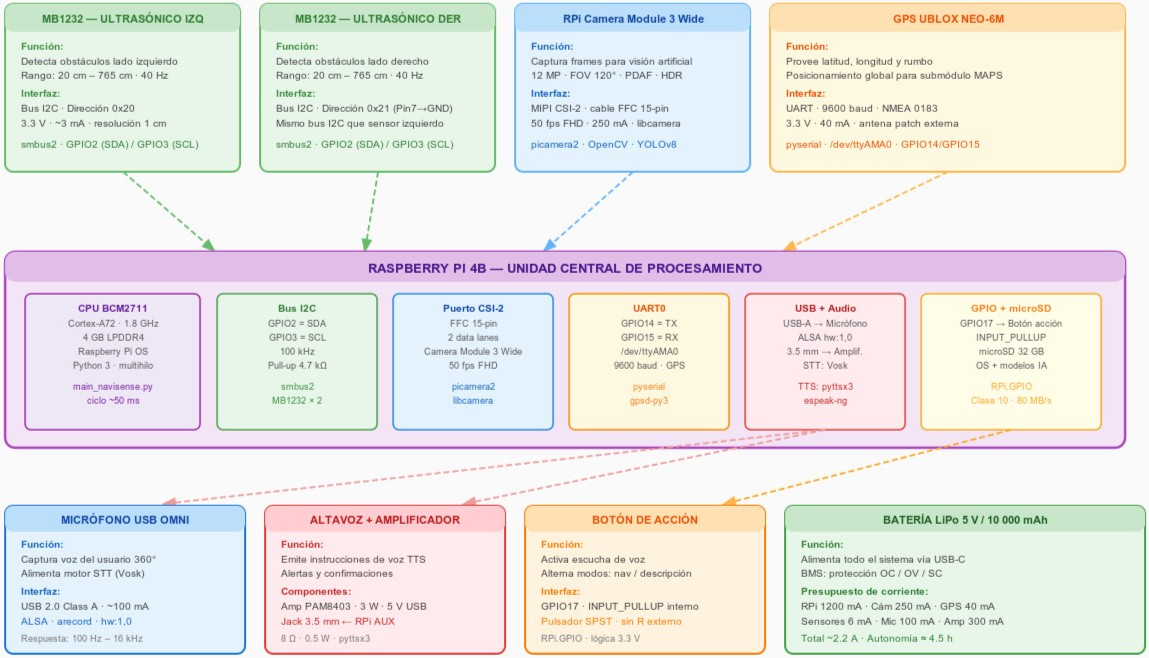
\includegraphics[width=0.8\textwidth]{Diagramas/electrosincables.jpg}
    \caption{Diagrama funcional de componentes electrónicos del sistema}
    \label{fig:bloques_electronica}
\end{figure}
 
La Figura~\ref{fig:conexiones_electronica} muestra el esquemático de conexiones
físicas del prototipo, donde se detallan los pines específicos de la Raspberry Pi
implicados en cada interfaz.
 
\begin{figure}[H]
    \centering
    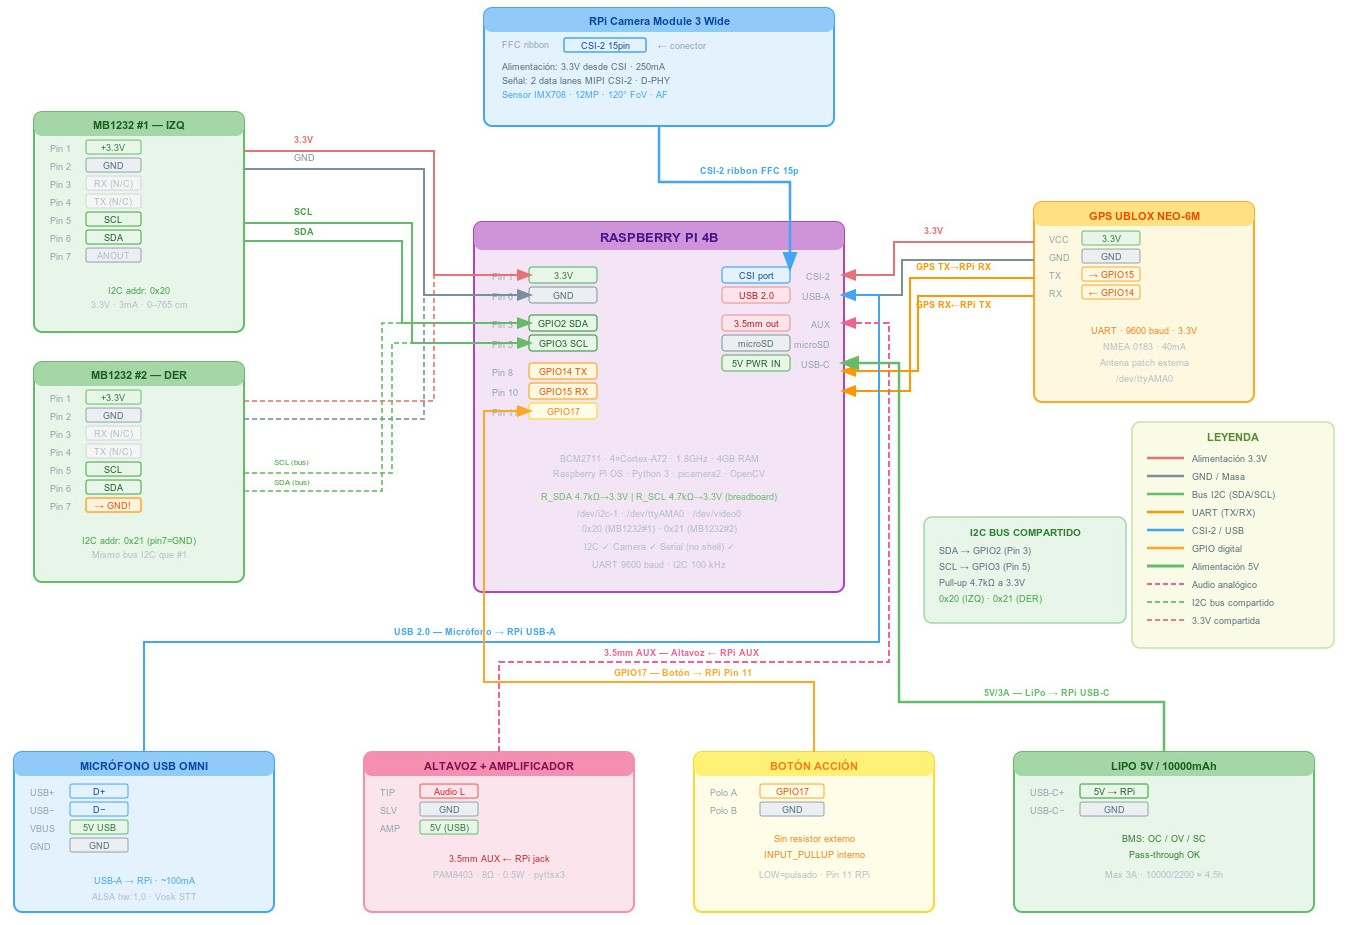
\includegraphics[width=0.88\textwidth]{Diagramas/electro.jpg}
    \caption{Esquemático de conexiones físicas del prototipo}
    \label{fig:conexiones_electronica}
\end{figure}

\subsection{Costos y viabilidad}

El sistema está diseñado para ejecutarse sobre hardware embebido de bajo costo,
siguiendo las restricciones establecidas en RNF-05 y RNF-10. La plataforma principal
es una Raspberry Pi, la cual ofrece la capacidad de procesamiento suficiente para
ejecutar la mayoría de los módulos del sistema bajo las latencias definidas en los
requerimientos. Sin embargo, debido a que algunas tareas como visión por computadora
o modelos de inteligencia artificial pueden demandar mayor capacidad de cómputo,
durante las pruebas se evaluará el desempeño general del sistema. En caso de detectar
limitaciones de rendimiento, se utilizará la conectividad Wi-Fi integrada de la
Raspberry Pi para establecer comunicación con una computadora personal que funcionará
como servidor de procesamiento, permitiendo ejecutar las tareas más pesadas de manera
remota sin modificar el funcionamiento general del sistema.

Para la percepción visual se selecciona el \textbf{Raspberry Pi Camera Module 3}, que
incorpora el sensor Sony IMX708 de 12~MP con tecnología CMOS \textit{back-illuminated
stacked}. Este módulo ofrece una buena calidad de imagen y resulta especialmente útil
en aplicaciones de visión por computadora debido a su sistema de autoenfoque y su
capacidad HDR, que ayudan a mantener imágenes más claras en diferentes condiciones
de iluminación, como cambios entre interiores y exteriores
\cite{raspberrypi_camera_doc3}. La versión Wide, con un campo de visión diagonal de
120°, permite capturar una mayor parte del entorno alrededor del usuario, lo cual es
ventajoso para navegación asistida y detección de obstáculos laterales. Además, su
compatibilidad nativa con Raspberry Pi y la biblioteca \texttt{libcamera} facilita
su integración con el sistema de procesamiento de imágenes
\cite{raspberrypi_camera_doc3}.

Para la detección de proximidad se utilizan \textbf{dos sensores MB1232}, colocados
en el frente del dispositivo, uno sobre cada cristal y apuntando en la misma dirección
que la cámara. Estos sensores fueron seleccionados debido
a que ofrecen lecturas más estables y confiables que alternativas más básicas como
el HC-SR04, especialmente en entornos urbanos donde puede existir ruido acústico o
eléctrico \cite{mb1232_datasheet}. Ambos sensores comparten el bus I2C de la
Raspberry Pi mediante la biblioteca \texttt{smbus2}, permitiendo una integración
compacta y sencilla. El MB1232 tiene un haz angosto, por lo que no es adecuado para
cubrir los costados; al frente, su haz coincide con lo que ve la cámara y permite
confirmar o descartar las detecciones visuales y detectar superficies que la visión no
reconoce, como vidrios y mamparas. La descripción de este montaje y su efecto en el
software se presenta en la Sección~\ref{sec:dev_prototipo}.

El sistema incorpora además un \textbf{botón para hablar}, que permite al usuario
activar o reiniciar la navegación sin depender completamente del reconocimiento de
voz. Esto resulta útil en ambientes con demasiado ruido o en situaciones donde el
usuario necesite interactuar rápidamente con el sistema.

La Tabla~\ref{tabla_hardware} detalla los componentes de hardware seleccionados para
el prototipo, junto con su función dentro del sistema, sus características principales
y su costo aproximado.

\begin{longtable}{p{4.2cm} p{4.5cm} p{2.8cm} p{1.8cm}}
\caption{Componentes de hardware del prototipo con costo aproximado}
\label{tabla_hardware} \\
\hline
\textbf{Componente} & \textbf{Función en el sistema}
    & \textbf{Especificación clave} & \textbf{Costo aprox.} \\
\hline
Raspberry Pi 4 Model B (4~GB RAM)
    & Unidad de procesamiento central. Ejecuta todos los módulos de software del sistema.
    & CPU quad-core Cortex-A72, 4~GB LPDDR4
    & \$75 USD \\
\hline
Raspberry Pi Camera Module 3 Wide (IMX708)
    & Captura continua de fotogramas para los módulos de percepción visual.
    & 12~MP, PDAF, HDR, FOV 120°, 50~fps FHD, CSI-2
    & \$25 USD \\
\hline
Sensor MB1232 I2CXL-MaxSonar (izquierda)
    & Medición de distancia al frente, sobre el cristal izquierdo. Dirección I2C
    \texttt{0x20}.
    & Rango 20~cm--765~cm, 1~cm res., I2C, 40~Hz
    & \$30 USD \\
\hline
Sensor MB1232 I2CXL-MaxSonar (derecha)
    & Medición de distancia al frente, sobre el cristal derecho. Dirección I2C
    \texttt{0x21}.
    & Rango 20~cm--765~cm, 1~cm res., I2C, 40~Hz
    & \$30 USD \\
\hline
Micrófono USB omnidireccional
    & Captura de audio para el módulo de reconocimiento de voz.
    & Respuesta 100~Hz -- 16~kHz, UAC class
    & \$15 USD \\
\hline
Altavoz + amplificador PAM8403 (3.5~mm)
    & Reproducción de instrucciones sintetizadas por el módulo de salida.
    & 8~$\Omega$, 0.5~W, conector AUX
    & \$10 USD \\
\hline
IMU de 9 ejes BNO055
    & Odometría del SLAM: orientación absoluta (giro) y aceleración lineal (conteo de
      pasos); inclinación de la cámara.
    & I2C \texttt{0x28}, fusión a bordo NDOF
    & \$35 USD \\
\hline
Botón de acción momentáneo
    & Activación o reinicio de sesión de navegación por hardware (GPIO17, pull-up interno).
    & SPST, lógica 3.3~V
    & \$2 USD \\
\hline
Batería LiPo 5~V 10000~mAh + BMS
    & Alimentación portátil del sistema completo vía USB-C. BMS con protección OC/OV/SC.
    & Corriente de salida máx. 3~A, pass-through
    & \$25 USD \\
\hline
Tarjeta microSD (32~GB, clase 10)
    & Almacenamiento del sistema operativo y modelos de IA.
    & Velocidad mínima 80~MB/s
    & \$10 USD \\
\hline
Resistencias pull-up 4.7~k$\Omega$ (×2)
    & Estabilización del bus I2C en líneas SDA y SCL.
    & 3.3~V, tolerancia 1\%
    & \$1 USD \\
\hline
\textbf{Total estimado} & & & \textbf{\$258 USD} \\
\hline
\end{longtable}
La estimación de costo total del prototipo es de aproximadamente \$258 USD, lo que lo
sitúa en un rango accesible para un prototipo de investigación de asistencia tecnológica.
El componente con mayor impacto en el costo son los sensores MB1232, cuyo precio unitario
supera al de los sensores ultrasónicos básicos, pero que se justifica por sus capacidades
de rechazo de ruido y calibración automática en tiempo real, necesarias para operar con
confiabilidad en los entornos ruidosos que describe la restricción RNF-06
\cite{mb1232_datasheet}. Los precios son estimaciones basadas en componentes disponibles
comercialmente y pueden variar según el proveedor y la región.

% Desarrollo realizado en TT2
\chapter{Desarrollo del sistema}
\label{cap:desarrollo}

En este capítulo se documenta el desarrollo realizado durante Trabajo Terminal II. El
capítulo de implementación de módulos recoge el diseño planteado en Trabajo Terminal I;
aquí se presenta lo que se construyó a partir de ese diseño, cómo se probó y qué
resultados dio. Se siguió la metodología incremental del marco metodológico
\cite{sommerville2011software}, así que cada módulo se implementó y probó por separado
antes de integrarlo con los demás. Varias decisiones del diseño original cambiaron en
el camino, conforme las mediciones mostraban qué funcionaba y qué no.

El orden del capítulo sigue el recorrido de la información dentro del sistema. Primero
se describe el prototipo físico y después la percepción (módulo de visión). Le siguen la
representación del entorno (SLAM, Ray Casting y mapeo), la toma de decisiones
(navegación y alertas) y, al final, la interacción por voz. En cada sección se explica
cómo quedó implementado el módulo, qué se midió y cuáles son sus limitaciones.

% ==============================================================================
\section{Entorno de desarrollo y organización del código}
% ==============================================================================

El software del sistema está escrito en Python~3. Para el cálculo matricial se usa
NumPy, para el manejo de imágenes OpenCV y para las gráficas y croquis Matplotlib. Cada
módulo vive en un archivo independiente y se comunica con los demás solo a través de
las estructuras de datos definidas en \texttt{interfaces.py}, lo que responde al
requerimiento de modularidad RNF-14. Gracias a eso, el SLAM no necesita saber si sus
observaciones vienen de la cámara del prototipo, de un video grabado o de la
simulación, y el mapa tampoco necesita saber cómo se estimó la pose que recibe. La
Tabla~\ref{tab:archivos_representacion} resume los archivos principales.

\begin{table}[H]
\centering
\caption{Archivos principales del código fuente}
\label{tab:archivos_representacion}
\renewcommand{\arraystretch}{1.25}
\begin{tabular}{|p{4.2cm}|p{10.3cm}|}
\hline
\textbf{Archivo} & \textbf{Responsabilidad} \\
\hline
\texttt{montaje.py} & Geometría física de los lentes: posición y orientación de la
cámara, de los ultrasónicos y de la IMU, y alcance del MB1232 según el tamaño del
objeto. \\
\hline
\texttt{vision\_bridge.py}, \texttt{vision/} & Módulo de visión: detección con YOLO,
segmentación de piso, puertas y peligros, rastreo de movimiento y fusión con el
ultrasonido. \\
\hline
\texttt{interfaces.py} & Estructuras compartidas entre módulos, desde la estimación de
movimiento hasta el cuadro de navegación. \\
\hline
\texttt{ekf\_slam.py} & Módulo SLAM: filtro de Kalman extendido sobre la pose,
asociación de datos y mapa ligero de \emph{landmarks}. \\
\hline
\texttt{odometry.py} & Estimación del movimiento con la IMU BNO055 (giro y conteo de
pasos), con respaldo por flujo óptico. \\
\hline
\texttt{occupancy\_grid.py} & Núcleo de Ray Casting: algoritmo de Bresenham, modelo
inverso del sensor en log-odds y rayos de consulta. \\
\hline
\texttt{map\_manager.py} & Módulo de mapeo: mapa global dividido en bloques
(\emph{chunks}), persistencia en disco, eventos de cambio de zona y capa de
peligros. \\
\hline
\texttt{navigation\_feed.py} & Construcción del cuadro que recibe el módulo de
navegación (distancias por sector, riesgos y mapa local). \\
\hline
\texttt{navigation/} & Módulo de navegación: entorno y script de entrenamiento con PPO,
ejecutor en el dispositivo, planificador de ruta y conversión de mapas reales en
mundos de entrenamiento. \\
\hline
\texttt{alertas.py} & Módulo de alertas y su conexión con los pitidos estéreo. \\
\hline
\texttt{interaccion.py}, \texttt{VozYPLN/} & Reconocimiento de voz, PLN, personalidad
del asistente, síntesis de voz y cola de mensajes con prioridades. \\
\hline
\texttt{main\_nav\_pi.py}, \texttt{main\_nav\_lap.py} & Programas principales del
sistema completo, uno para la Raspberry Pi del prototipo y otro para la computadora
portátil, con interfaz gráfica. \\
\hline
\texttt{video\_a\_mapa.py} & Conversión de videos grabados en primera persona en mapas
guardados. \\
\hline
\texttt{sim\_world.py}, \texttt{tests/} & Banco de simulación, métricas y pruebas
automatizadas. \\
\hline
\end{tabular}
\end{table}

% ==============================================================================
\section{Cambios respecto al diseño de Trabajo Terminal I}
% ==============================================================================

Durante el desarrollo se tomaron decisiones que modifican lo planteado en TT1. Casi
todas surgieron al medir el comportamiento de los módulos, y en todos los casos el
código fuente es la referencia vigente. La Tabla~\ref{tab:cambios_tt1} reúne los
cambios principales.

\begin{longtable}{|p{3.0cm}|p{5.4cm}|p{6.1cm}|}
\caption{Cambios respecto al diseño de TT1}
\label{tab:cambios_tt1} \\
\hline
\textbf{Aspecto} & \textbf{Diseño en TT1} & \textbf{Implementación en TT2} \\
\hline
\endfirsthead
\hline
\textbf{Aspecto} & \textbf{Diseño en TT1} & \textbf{Implementación en TT2} \\
\hline
\endhead
Navegación global & Rutas a nivel ciudad con un servicio de cartografía digital y
GPS NEO-6M. & Se descartó. Los destinos se buscan entre los \emph{landmarks}
etiquetados del propio mapa (por ejemplo, ``la salida'' se resuelve como una puerta),
sin depender de internet ni de señal satelital. \\
\hline
Observaciones del EKF & Lecturas de los sensores de proximidad comparadas contra
el mapa de ocupación. & Rango y dirección hacia \emph{landmarks} detectados por la
cámara, refinados con el ultrasonido cuando ambos coinciden. Los ecos aislados no
corrigen la pose. \\
\hline
Estado del filtro & Pose $[x, y, \theta]$. & Se conserva la pose de tres variables y
los \emph{landmarks} se guardan en una lista aparte, con su propio modelo de
incertidumbre. \\
\hline
Odometría & ``Odometría aproximada'' sin especificar. & IMU BNO055 con orientación
fusionada a bordo y conteo de pasos, con respaldo automático por flujo óptico. \\
\hline
Mapa & Una sola retícula local. & Mapa global dividido en bloques de
$8 \times 8$~m que se cargan y descargan según se necesiten, se guardan entre
sesiones y avisan de los cambios de cuarto. \\
\hline
Ray Casting & Celdas recorridas libres y celda final ocupada. & Se agregaron reglas
para el rango impreciso, las paredes ya consolidadas, los rayos sin eco y los
peligros de piso, que van en una capa separada. \\
\hline
Salida hacia navegación & Matriz 2D del entorno. & Cuadro de navegación con la pose,
su incertidumbre, un mapa local de dos canales, las distancias y riesgos por sector y
los \emph{landmarks} etiquetados. \\
\hline
Ultrasonido & Dos MB1232 que cubren los laterales del usuario. & Dos MB1232 al frente,
uno sobre cada cristal, que validan las detecciones de la cámara, estiman de qué lado
está el obstáculo y descartan los ecos del piso. \\
\hline
Visión & YOLOv8 con preprocesamiento de contraste y suavizado. & Tres modelos
preentrenados: YOLOv8s-seg (COCO), YOLOv8s (Open Images) para puertas, escaleras y
muebles, y SegFormer (ADE20K) para piso, puertas y peligros. \\
\hline
Observación del agente & Vector de 8 valores. & Vector de 24 valores (11 rayos,
peligros, riesgos, meta y acción previa), elegido por comparación directa. \\
\hline
Seguridad de la navegación & Alertas que fuerzan el recálculo. & Además, una capa
determinística que anula la orden de avanzar con el frente bloqueado, y alertas
activas aunque no haya ruta. \\
\hline
Voz y PLN & Detección de actividad de voz, filtro de Wiener, Vosk, spaCy y pyttsx3. &
Vosk detecta por sí mismo el final de cada frase, el PLN es propio (reglas más una red
neuronal) y la voz es neuronal con respaldo local. Se añadió una personalidad para el
asistente. \\
\hline
\end{longtable}

% ==============================================================================
\section{Metodología de pruebas}
\label{sec:validacion_representacion}
% ==============================================================================

El sistema se probó en tres niveles. Las pruebas con el prototipo armado muestran el
comportamiento real de los lentes; el banco de simulación permite medir el error con
exactitud, porque ahí sí se conoce la posición verdadera; y los videos grabados en
primera persona sirven para ver el sistema en lugares reales y variados sin tener que
recorrerlos cada vez con el prototipo. Algunos módulos tuvieron además pruebas
propias, como la evaluación del agente de navegación en 880 episodios, las sesiones
completas en lazo cerrado y la evaluación del reconocimiento de voz, que se describen
en su sección.

\textbf{Prototipo.} \TODO{describir las pruebas con el prototipo armado: lugares,
número de recorridos, participantes y condiciones de luz y ruido}.

\textbf{Banco de simulación.} Es un cuarto virtual de $6 \times 4$~m con cinco
obstáculos (una mesa, dos sillas, un sillón y una maceta) en el que un usuario simulado
recorre una secuencia de puntos. El banco genera odometría con ruido, las lecturas de
los dos ultrasónicos frontales colocados como en el prototipo y detecciones visuales
con un error de dirección de $2^\circ$ y un error de distancia del 25\,\%, parecido al
de la estimación monocular. El flujo de datos es el mismo que en el prototipo; lo único
que cambia es de dónde vienen los datos.

\textbf{Videos reales.} Se grabaron 19 recorridos en primera persona con teléfonos
celulares ($1920 \times 1080$ a 30 cuadros por segundo) en calles, banquetas, una
casa, una plaza comercial, oficinas y la sala de maestros de la escuela. Cada video se
procesó con el mismo flujo del prototipo para generar mapas y capturas. Como en estos
casos no hay una referencia exacta, la evaluación es cualitativa y se basa en qué tan
bien se parece el mapa al lugar recorrido.

\textbf{Pruebas automatizadas.} El código tiene 205 pruebas unitarias y funcionales en
la carpeta \texttt{tests/}. Hay 33 del SLAM, 36 del mapa, 34 de la navegación, 26 de
las alertas y el planificador, 22 del montaje de los sensores y la validación cruzada,
24 de la interacción, 5 del PLN, 15 de la visión y 10 de la odometría. Todas corren sin hardware y
todas pasan.

Para el SLAM se usa el error absoluto de trayectoria (ATE), que es la distancia
promedio entre la posición estimada y la real a lo largo del recorrido y es la métrica
habitual para evaluar estos sistemas \cite{sturm2012tum}:

\[
\text{ATE} = \frac{1}{N}\sum_{t=1}^{N}
\sqrt{(\hat{x}_t - x_t)^2 + (\hat{y}_t - y_t)^2}
\]

También se reporta el error medio de orientación, con la diferencia angular normalizada
al intervalo $(-\pi, \pi]$. La calidad del mapa se mide con la precisión, que es la
proporción de celdas marcadas como ocupadas que de verdad corresponden a un obstáculo,
y con la exhaustividad (\emph{recall}), que es la proporción de las superficies reales
que quedaron registradas. En ambas se acepta una tolerancia de dos celdas (10~cm),
porque exigir la celda exacta castigaría errores más chicos que el propio ruido de los
sensores. Por último, se mide el tiempo de procesamiento por ciclo para revisar RNF-03
y RNF-05.

Las figuras y tablas de resultados de este capítulo se generan directamente del código
con los scripts \texttt{tests/figuras\_doc.py}, \texttt{tests/figuras\_doc\_vision.py},
\texttt{tests/figuras\_doc\_nav.py} y \texttt{tests/eval\_interaccion.py}, así que
pueden reproducirse. Los tiempos de los experimentos de simulación y video se midieron
en una computadora portátil con procesador Apple M4; los del prototipo se indican en
cada sección.

% ==============================================================================
\section{Prototipo físico}
\label{sec:dev_prototipo}
% ==============================================================================

El armazón de los lentes se diseñó en un modelador CAD. Los sensores definidos en la
sección de electrónica de TT1 van alojados en un frente ensanchado, por encima de los
cristales, y las patillas son anchas para dar espacio al cableado. La
Figura~\ref{fig:proto_explosivo} muestra la vista explosionada. La Camera Module 3 Wide
va en el centro del frente, a la altura del puente de la nariz, de modo que queda
alineada con la dirección en la que mira el usuario; el módulo de visión y el cálculo de
distancias por plano de piso parten de esa suposición. Los dos sensores ultrasónicos
MB1232 van en el frente, uno sobre cada cristal, y la IMU BNO055 va plana en la parte
superior del mismo frente. El resto de las tarjetas se aloja detrás de la cámara y en la
patilla derecha, donde queda un conector accesible desde el exterior.

\begin{figure}[H]
    \centering
    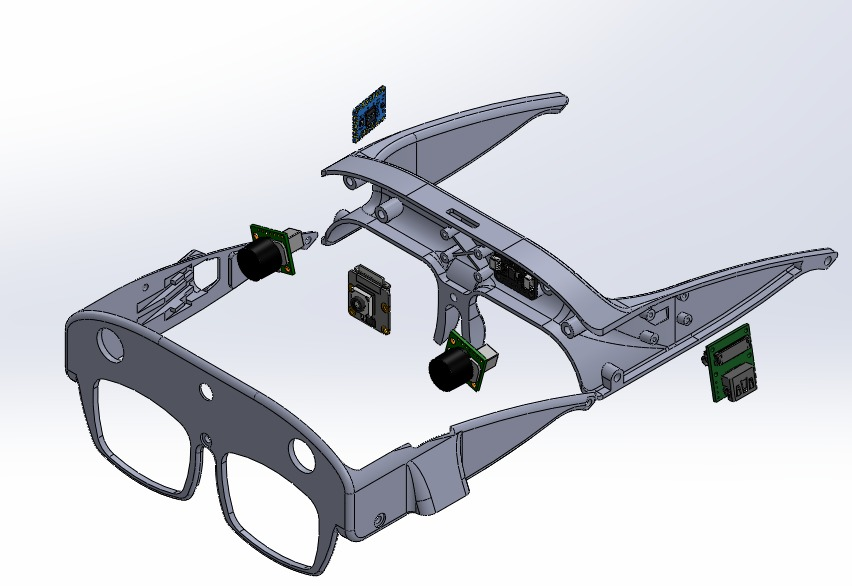
\includegraphics[width=0.85\textwidth]{Capturas_TT2/hardware/Render.jpeg}
    \caption{Vista explosionada del armazón, con la cámara al centro y los sensores
    ultrasónicos sobre cada cristal.}
    \label{fig:proto_explosivo}
\end{figure}

Las Figuras~\ref{fig:proto_transparente} y \ref{fig:proto_armado} muestran el diseño
armado, primero con el frente transparente para ver la disposición interna y después
con el acabado final.

\begin{figure}[H]
    \centering
    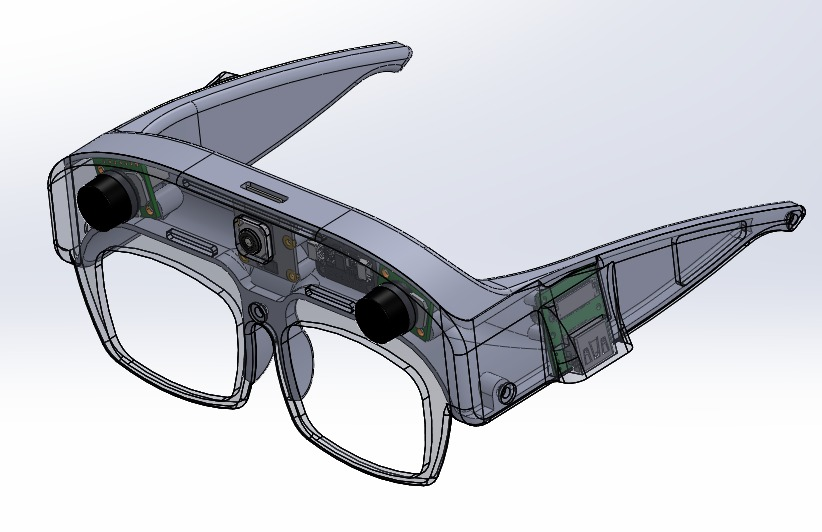
\includegraphics[width=0.8\textwidth]{Capturas_TT2/hardware/VistaPrincipal.jpeg}
    \caption{Diseño armado con el frente transparente.}
    \label{fig:proto_transparente}
\end{figure}

\begin{figure}[H]
    \centering
    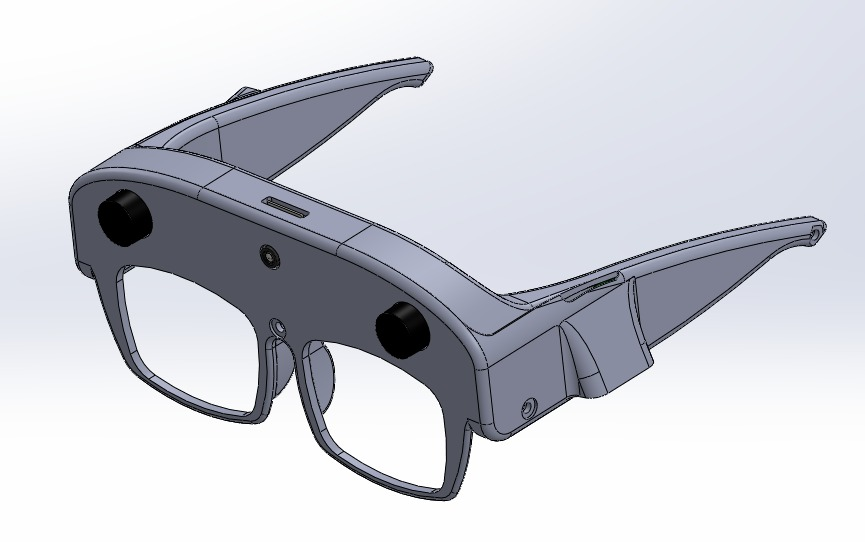
\includegraphics[width=0.8\textwidth]{Capturas_TT2/hardware/VistaReal.jpeg}
    \caption{Diseño armado con el acabado final.}
    \label{fig:proto_armado}
\end{figure}

\TODO{agregar fotos del prototipo fabricado y armado, y describir el material, el
método de fabricación, el peso final y dónde van la Raspberry Pi y la batería}.

Los dos ultrasónicos apuntan hacia adelante, en la misma dirección que la cámara, y
están separados unos 10~cm. Como los sensores y la IMU van en el mismo frente rígido, el
cabeceo que mide la IMU es también el de la cámara y el de los ultrasónicos. Toda esta
geometría se concentra en un solo archivo, \texttt{montaje.py}, que usan el driver de
los sensores, la fusión, las alertas y el simulador, y que se ajusta con las medidas
tomadas sobre el prototipo.

En TT1 se había planteado que los ultrasónicos cubrieran los costados del usuario. Al
revisar la hoja de datos se vio que el MB1232 tiene un haz angosto, de unos
$\pm 14^\circ$, así que sirve poco para vigilar los lados. Puesto al frente, en cambio,
su haz coincide con lo que ve la cámara. Eso permite confirmar o descartar las
detecciones visuales, avisar de vidrios y mamparas que la cámara no reconoce y corregir
el estado de las puertas, como se explica en las secciones de SLAM, visión y alertas.
El costo de esta decisión es que los costados quedan cubiertos solo por la cámara y que
el mapa registra menos superficie lateral (Tabla~\ref{tab:mapeo_us}).


% ==============================================================================
\section{Módulo de visión}
\label{sec:dev_vision}
% ==============================================================================

\subsection{Descripción}

El módulo de visión recibe cada cuadro de la cámara y entrega una lista de
detecciones. Para cada objeto se indica qué es, en qué dirección está respecto al frente
del usuario, a qué distancia aproximada se encuentra, si se está moviendo y, en el caso
de las puertas, si está abierta o cerrada. Con esa lista trabajan el SLAM, las alertas y
la descripción del entorno que el usuario puede pedir por voz. El módulo atiende los
requerimientos RF-07 a RF-10 y RF-13.

En TT1 el módulo se planteó alrededor de un solo detector, YOLOv8. Al probarlo con los
videos reales salió a la luz su mayor carencia, pues el conjunto COCO con el que viene
entrenado no incluye puertas, escaleras ni escritorios, que son justamente los objetos
que más ayudan a orientarse dentro de un edificio. Por eso la versión final combina tres
modelos preentrenados, cada uno con una tarea distinta, como se resume en la
Tabla~\ref{tab:vision_modelos}.

\begin{table}[H]
\centering
\caption{Modelos que componen el módulo de visión}
\label{tab:vision_modelos}
\renewcommand{\arraystretch}{1.25}
\begin{tabular}{|p{3.4cm}|p{3.1cm}|p{2.3cm}|p{5.7cm}|}
\hline
\textbf{Modelo} & \textbf{Entrenamiento} & \textbf{Frecuencia} & \textbf{Uso} \\
\hline
YOLOv8s-seg & COCO, 80 clases & Cada cuadro & Personas, vehículos, muebles y objetos
comunes \cite{redmon2016yolo}. \\
\hline
YOLOv8s & Open Images V7, 600 clases & Cada 5 cuadros (15 en la Raspberry Pi) & Solo
las clases que COCO no tiene, como puerta, escalera, ventana, bote de basura, poste,
letrero, árbol, escritorio, archivero o pizarrón. \\
\hline
SegFormer-B0 & ADE20K, 150 clases & Cada 4 a 10 cuadros & Segmentación de la escena
para encontrar piso transitable, agua, escaleras y puertas \cite{xie2021segformer,
zhou2017ade20k}. \\
\hline
\end{tabular}
\end{table}

\subsection{Preprocesamiento y geometría de la cámara}

Cada cuadro se reduce a 640 píxeles de ancho conservando su relación de aspecto. Una
versión anterior lo forzaba a $640 \times 480$; en los videos 16:9 eso estiraba la
imagen en vertical, inflaba la altura de las cajas y hacía que las distancias salieran
cerca de un 25\,\% más cortas. Ahora la dirección, la distancia por altura típica y la
distancia por plano de piso se calculan con una sola distancia focal, obtenida del campo
de visión horizontal. Hay dos perfiles de cámara, uno para la cámara web de la
computadora portátil ($70^\circ$) y otro para la Camera Module 3 Wide del prototipo
($102^\circ$). Las ecuaciones de distancia se presentan en la Sección~\ref{sec:dev_slam};
el rango estimado se acota entre 0.2 y 8~m.

La igualación de histograma y el filtro gaussiano del pseudocódigo de TT1
(Apéndice~\ref{apend:procesa}) se dejaron fuera. Los modelos preentrenados ya normalizan
la imagen por dentro y, en las pruebas con video, esos pasos no mejoraron nada que
justificara su costo por cuadro.

\subsection{Detección de objetos}

El detector principal es YOLOv8s-seg con un umbral de confianza de 0.45. Algunas
etiquetas de COCO se renombran para que coincidan con el resto del sistema (por ejemplo,
\emph{couch} pasa a \emph{sofa} y \emph{tv} a \emph{monitor}). El detector de Open
Images se ejecuta con un umbral de 0.25 y solo cada cierto número de cuadros, porque en
CPU cuesta casi lo mismo que el principal. De sus 600 clases se conservan nada más las
que aportan algo nuevo, y si una de sus cajas se encima con una de COCO con un IoU mayor
a 0.55, se descarta para no contar dos veces el mismo objeto. La lista de clases creció
después de una prueba en la sala de maestros de la escuela, donde el sistema casi no
detectaba nada porque los escritorios y archiveros no existían en COCO.

\subsection{Puertas, piso y peligros por segmentación}

SegFormer asigna una clase a cada píxel de la imagen, y de ese mapa se sacan tres tipos
de información. La primera son las puertas. Cada región conexa de la clase puerta que
ocupa al menos el 0.4\,\% de la imagen se convierte en una detección, y se considera
abierta si dentro de su recuadro hay más de un 7\,\% de piso transitable, es decir, si a
través del vano se alcanza a ver el piso del otro lado. Cuando el detector de Open
Images ya vio una puerta en la misma dirección (con menos de $8^\circ$ de diferencia),
se conserva solo una. Además, si la puerta queda dentro del haz de los ultrasónicos, el
eco decide su estado, como se explica en la Sección~\ref{sec:dev_slam}.

La segunda son el agua y las escaleras, que ADE20K reconoce como clases propias. Se
toman las regiones que aparecen en el 55\,\% inferior de la imagen y se ubican con la
distancia por plano de piso. La tercera son los hoyos y coladeras, para los que no
existe una clase. Se detectan como regiones no transitables rodeadas de piso, con
varias condiciones para evitar confusiones; la región debe estar en la parte baja de la
imagen, ocupar entre el 0.15 y el 20\,\% del cuadro, no tocar los bordes y estar rodeada
de piso transitable en al menos un 55\,\% de su contorno. Si un peligro coincide en
dirección y distancia con un objeto que ya detectó YOLO, se descarta, porque casi
siempre se trata de la sombra o la base de ese mismo objeto.

\subsection{Objetos en movimiento}

El rastreador de \texttt{vision/motion.py} asocia las cajas entre cuadros y guarda el
historial de sus centroides; si un objeto se desplaza más de 8 píxeles, se marca como
móvil. Las personas, los animales y los vehículos se marcan siempre como móviles. En la
primera versión, cada vez que el usuario giraba la cabeza todo el cuarto parecía
moverse. Para corregirlo, antes de comparar se desplaza el historial del rastreador lo
que corresponde al giro medido por la odometría, $\Delta u = \Delta\theta \cdot W /
\text{FOV}_h$, y así solo queda el movimiento propio de los objetos.

\subsection{Nivel de riesgo}

Cada detección recibe un nivel de riesgo de 0 a 3 según la tabla definida en TT1
(Tabla~\ref{tabla_riesgo}). Los peligros de piso y los objetos en movimiento tienen
riesgo alto (3), los obstáculos estáticos y las puertas cerradas riesgo medio (2), y las
puertas abiertas y las paredes riesgo bajo (1). El mapeo agrupa estos niveles por sector
para construir $r_{\text{front}}$, $r_{\text{left}}$ y $r_{\text{right}}$.

\subsection{Resultados}

La Figura~\ref{fig:vision_escenas} muestra el módulo trabajando sobre tres escenas de
los videos reales. A la izquierda se marcan las detecciones con su distancia estimada
(en verde los objetos estáticos, en rojo los móviles y en magenta los peligros de piso)
y a la derecha la segmentación, con el piso transitable en verde, las puertas en azul y
las paredes en gris.

\begin{figure}[H]
    \centering
    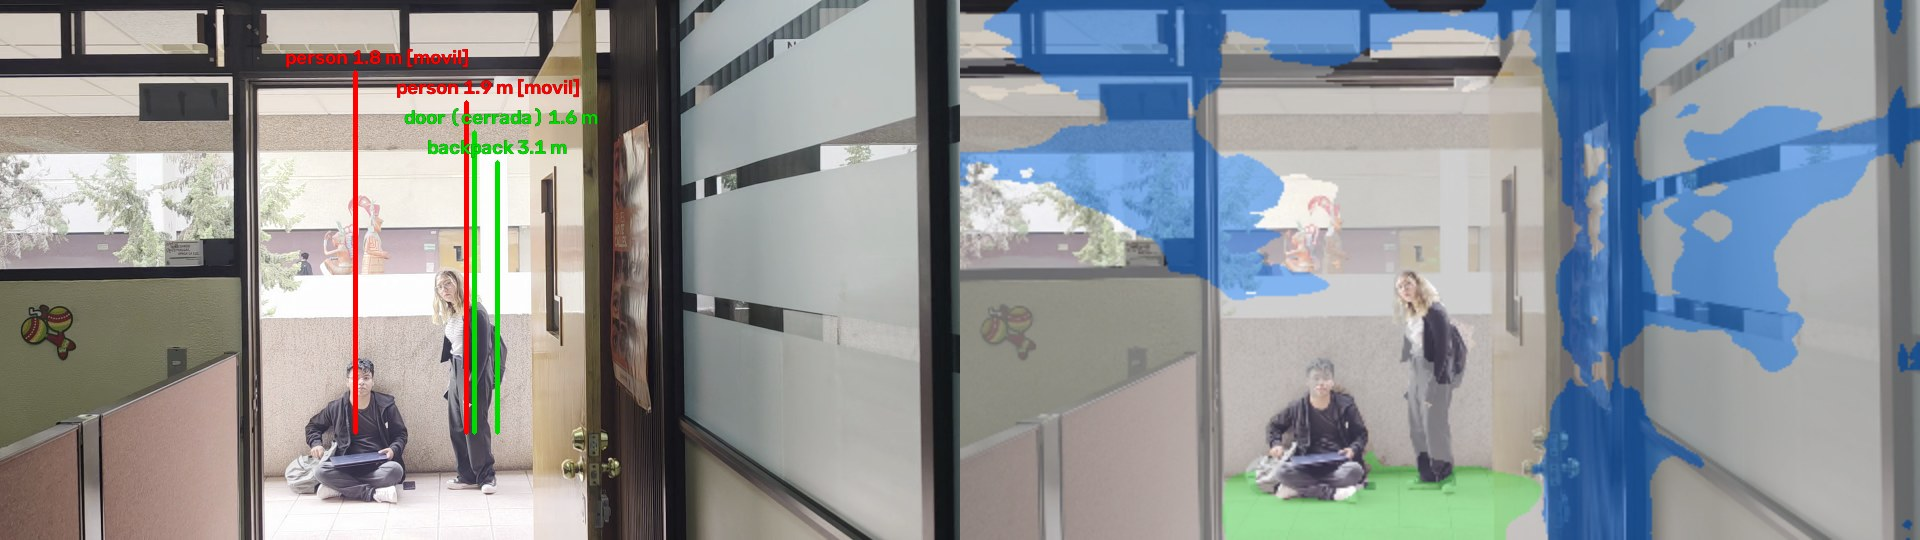
\includegraphics[width=\textwidth]{Capturas_TT2/vision/vision_escena11.jpg}\\[2pt]
    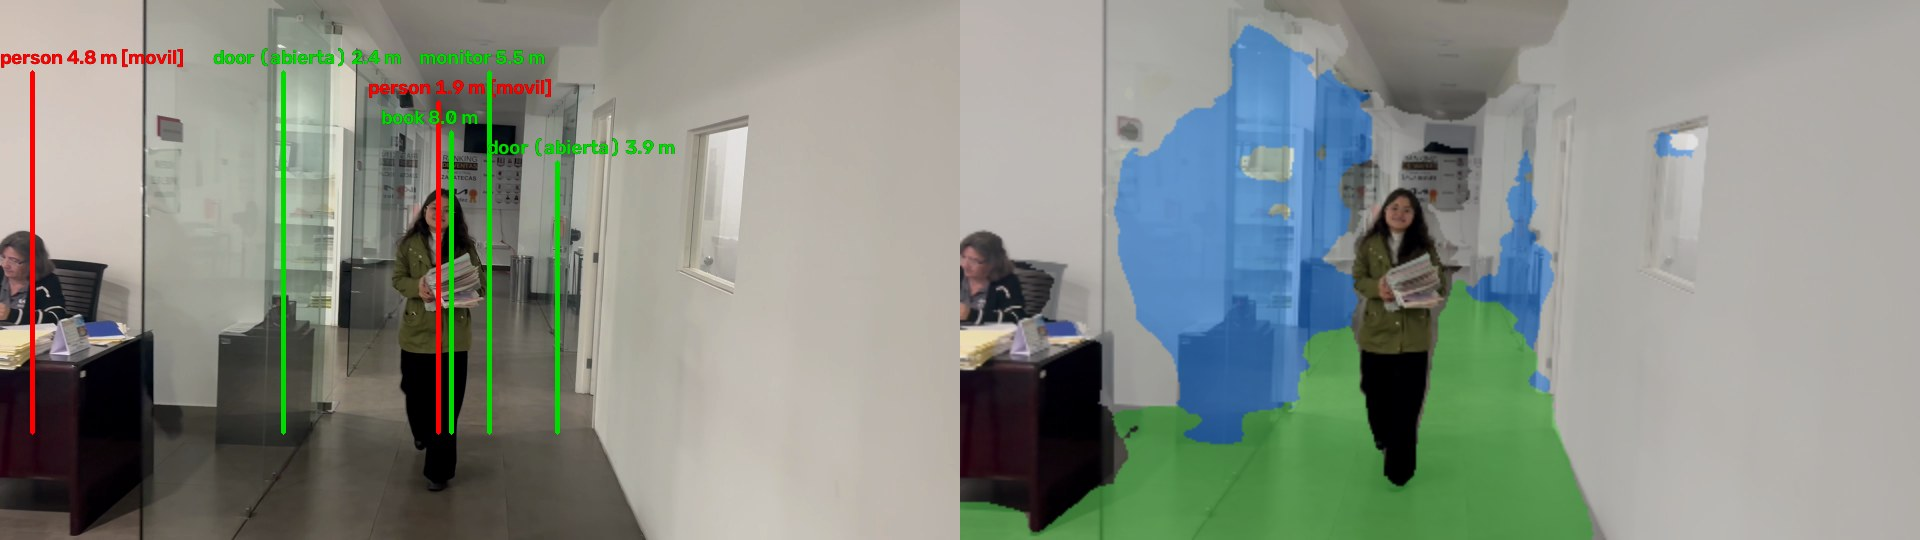
\includegraphics[width=\textwidth]{Capturas_TT2/vision/vision_escena14.jpg}\\[2pt]
    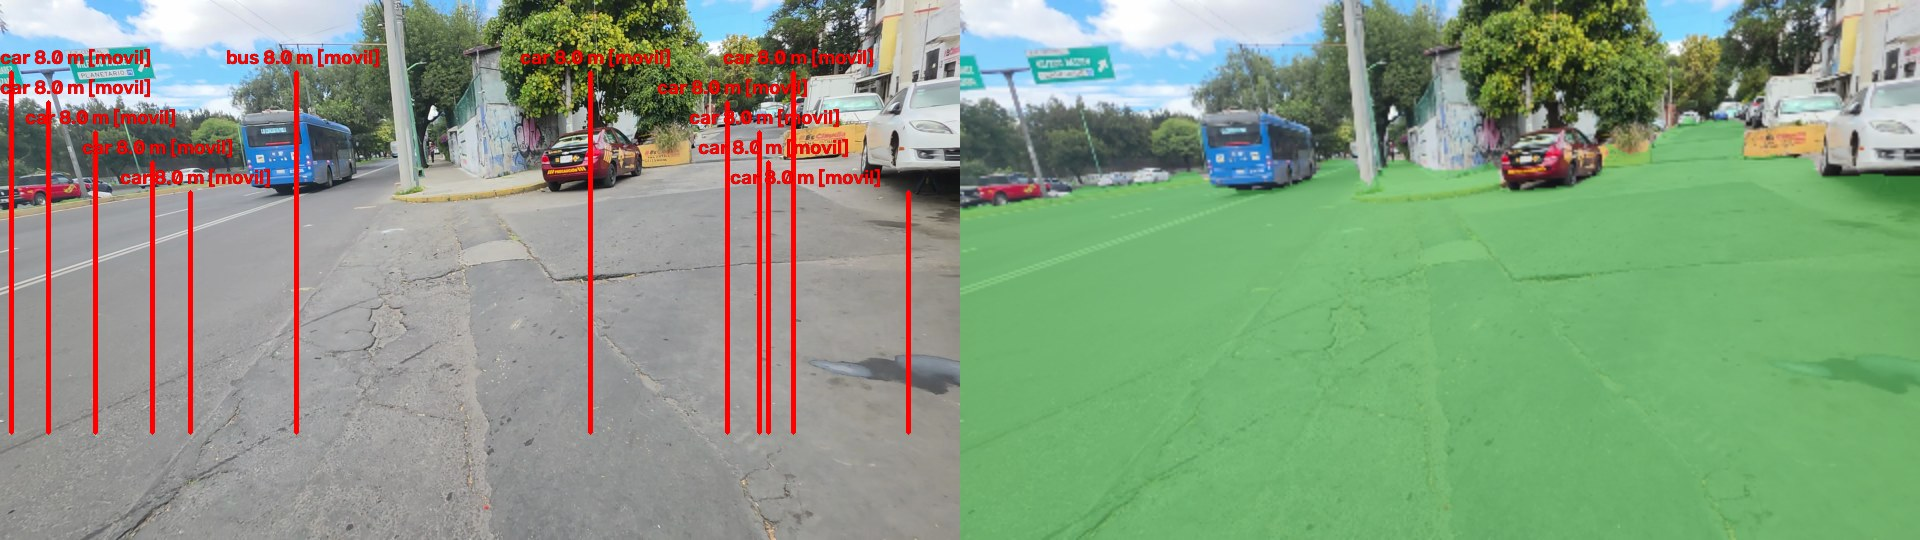
\includegraphics[width=\textwidth]{Capturas_TT2/vision/vision_escena6.jpg}
    \caption{Detecciones (izquierda) y segmentación (derecha) en la entrada de la sala
    de maestros, en un pasillo de oficina con una persona caminando y en una calle con
    vehículos.}
    \label{fig:vision_escenas}
\end{figure}

En la entrada de la sala de maestros el sistema detecta a las dos personas, una mochila
y la puerta, que clasifica como cerrada a 1.6~m. En el pasillo de oficina detecta a la
persona que camina hacia la cámara (a 1.9~m), un monitor y dos puertas abiertas, aunque
la segmentación también marca como puerta buena parte de los canceles de vidrio, así que
al menos una de esas ``puertas'' es en realidad una mampara. La señora sentada en el
escritorio aparece a 4.8~m cuando está a unos 2~m; la distancia se calcula con la altura
típica de una persona de pie (1.65~m), y alguien sentado se ve más bajo, lo que el
modelo interpreta como lejanía. En la calle, los vehículos aparecen como móviles y a
8~m, que es el tope del rango. Más delicado es que la segmentación pinta como piso
transitable tanto la banqueta como el arroyo vehicular, porque la clase \emph{road} de
ADE20K está entre las superficies transitables, y que los baches del pavimento no se
reportan como peligro.

La Figura~\ref{fig:vision_tapete} muestra un falso positivo típico. Un tapete con un
estampado oscuro sobre un piso claro cumple todas las condiciones de un hoyo, porque la
segmentación no lo reconoce como piso, está en la parte baja de la imagen y tiene piso
alrededor. El sistema lo reporta como hoyo a 0.9~m.

\begin{figure}[H]
    \centering
    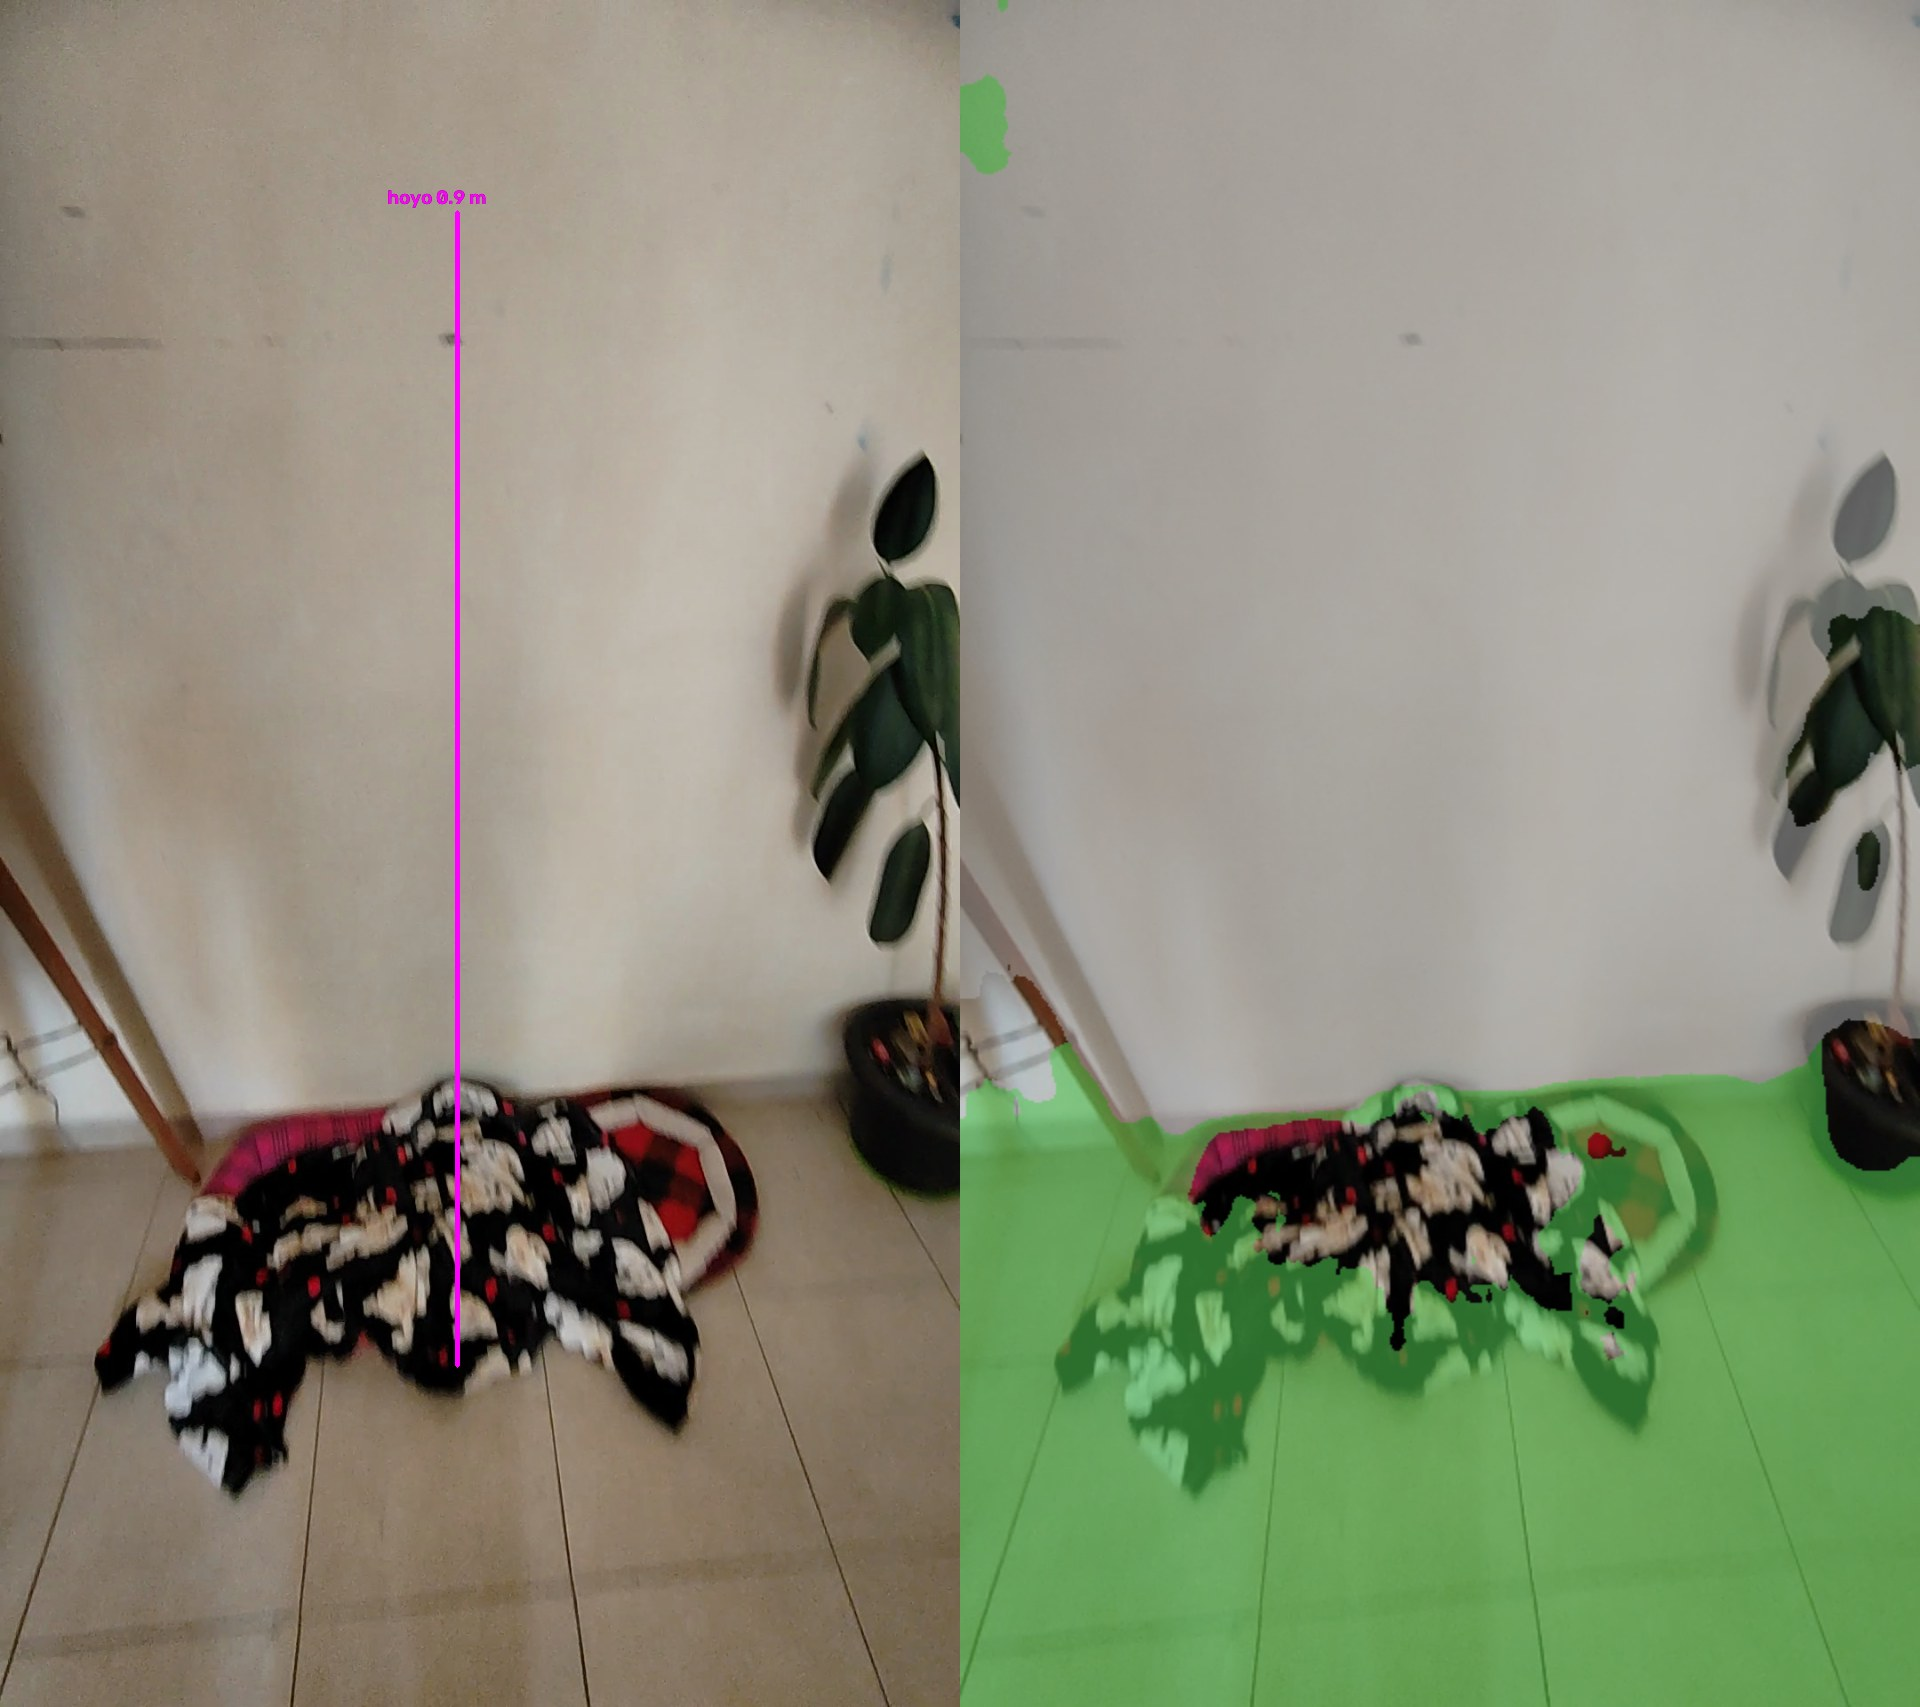
\includegraphics[width=0.62\textwidth]{Capturas_TT2/vision/vision_escena16.jpg}
    \caption{Falso positivo: un tapete estampado se detecta como hoyo a 0.9~m.}
    \label{fig:vision_tapete}
\end{figure}

La Tabla~\ref{tab:vision_tiempos} reporta el tiempo de inferencia de cada modelo,
medido en CPU sobre el mismo cuadro, en la computadora portátil y en la Raspberry Pi del
prototipo.

\begin{table}[H]
\centering
\caption{Tiempo de inferencia por modelo (promedio de 10 ejecuciones)}
\label{tab:vision_tiempos}
\renewcommand{\arraystretch}{1.2}
\begin{tabular}{|l|c|c|c|}
\hline
\textbf{Modelo} & \textbf{Entrada} & \textbf{Apple M4 (ms)} &
\textbf{Raspberry Pi (ms)} \\
\hline
YOLOv8s-seg (COCO) & $640 \times 360$ & 72 & \TODO{} \\
YOLOv8s (Open Images V7) & $640 \times 360$ & 55 & \TODO{} \\
SegFormer-B0 con puertas y peligros & $480 \times 270$ & 293 & \TODO{} \\
\hline
\end{tabular}
\end{table}

En la computadora portátil, con el detector principal en cada cuadro, el extra cada
cinco y la segmentación cada cuatro, el costo promedio es de unos 160~ms por cuadro, o
sea, unos 6 cuadros por segundo. La segmentación es lo más caro; por eso se ejecuta con
menos frecuencia y sus resultados se reutilizan en los cuadros intermedios. En la
Raspberry Pi, con la configuración del prototipo (extra cada 15 cuadros y segmentación
cada 10), el sistema procesa \TODO{cuadros por segundo en la Raspberry Pi}.

La precisión de detección que pide RNF-06 se mide sobre imágenes tomadas con la
cámara del prototipo y etiquetadas a mano. \TODO{armar el conjunto y reportar número de
imágenes, clases, precisión y exhaustividad}. Para mejorar las clases propias del
entorno se cuenta con el script \texttt{vision/finetune.py}, que reentrena YOLO con un
conjunto en formato YOLO. \TODO{resultado del reentrenamiento con puertas y mamparas de
la escuela, si se realiza}. El módulo tiene 15 pruebas automatizadas que usan detectores
simulados para revisar la geometría, las puertas, el detector extra y la eliminación de
duplicados.

\subsection{Limitaciones}

Ninguno de los tres modelos tiene una clase para mamparas o canceles de vidrio. La
segmentación a veces los toma por puertas y a veces no los ve; los ultrasónicos
frontales compensan en parte, porque un eco sin detección visual se avisa como pared y
el eco corrige el estado de las puertas de vidrio, pero solo dentro de su cono angosto.
El criterio geométrico de los hoyos también genera falsos positivos con tapetes,
manchas y cambios de textura del piso.

El rastreador compensa el giro del usuario, pero no su avance. Al caminar hacia
adelante, las cajas de los objetos cercanos crecen y algunos objetos estáticos se marcan
como móviles, como se ve en la Figura~\ref{fig:cap_oficina_3}. La distancia monocular,
por su parte, depende de la altura típica de cada clase, de modo que una persona sentada
o un objeto de tamaño poco común quedan mal ubicados, y se satura en 8~m. Por último, la
calle se considera tan transitable como la banqueta y los baches poco profundos no se
distinguen del pavimento, así que en exteriores el sistema no sabe por sí solo que bajar
al arroyo vehicular es peligroso. \TODO{separar banqueta y arroyo vehicular en la
segmentación}.


% ==============================================================================
\section{Módulo de SLAM}
\label{sec:dev_slam}
% ==============================================================================

\subsection{Descripción y alcance}

El módulo de SLAM responde en cada ciclo una pregunta sencilla de plantear y difícil de
resolver, que es dónde está el usuario y hacia dónde mira dentro del mapa que se va
construyendo. Ningún sensor entrega esa respuesta de manera directa. La cámara da la
dirección de los objetos con buena precisión, pero su distancia con mucho error; el
ultrasonido mide distancias exactas, pero solo hacia el frente; y cualquier estimación
de movimiento acumula error con el tiempo. El SLAM junta estas fuentes, lleva la cuenta
de qué tanto se puede confiar en la pose y la entrega a los módulos de Ray Casting y
mapeo. Con ello cubre RF-14 y RF-15.

En TT1 se planteó un SLAM ``simplificado'' basado en un filtro de Kalman extendido
(EKF) \cite{kalman1960, thrun2005probabilistic}, y esa idea se mantuvo, aunque hubo que
precisar la variante. En el EKF-SLAM clásico \cite{smith1990uncertain} el vector de
estado incluye la pose y la posición de cada \emph{landmark}, de modo que la matriz de
covarianza crece con el cuadrado del número de elementos del mapa
\cite{bailey2006slam2}. Los sistemas de SLAM visual como ORB-SLAM
\cite{murartal2015orbslam}, por su parte, siguen miles de puntos característicos y
piden más cómputo del que una Raspberry Pi puede dar mientras también ejecuta la
detección de objetos.

Por eso el estado del filtro contiene solo la pose, $\boldsymbol{\mu} = [x,\; y,\;
\theta]^T$, con una covarianza $\mathbf{P}$ de $3 \times 3$, y el costo de cada ciclo es
el mismo sin importar cuántos objetos haya en el mapa. Los \emph{landmarks} se guardan
en una lista ligera fuera del filtro, cada uno con su posición, su etiqueta (silla,
puerta, mesa, etc.) y el número de veces que se ha visto. Al corregir, el filtro usa el
\emph{landmark} asociado como referencia y suma su incertidumbre de posición, que baja
con cada nueva observación, a la covarianza de la innovación; así no trata a un objeto
recién visto como si su posición fuera exacta. En términos académicos, la variante
corresponde a un EKF de localización con mapeo incremental de apoyo. Se privilegia una
pose barata y estable, y el mapa de ocupación lo refinan después los módulos de Ray
Casting y mapeo con la pose que el SLAM les entrega.

\subsection{Entradas y salidas}

La Tabla~\ref{tab:slam_interfaces} describe las estructuras de datos que intercambia el
módulo, definidas en \texttt{interfaces.py}.

\begin{table}[H]
\centering
\caption{Interfaces del módulo de SLAM}
\label{tab:slam_interfaces}
\renewcommand{\arraystretch}{1.25}
\begin{tabular}{|p{3.3cm}|p{1.6cm}|p{9.6cm}|}
\hline
\textbf{Estructura} & \textbf{Tipo} & \textbf{Contenido} \\
\hline
\texttt{MotionEstimate} & Entrada & Desplazamiento $\Delta d$ (m), giro $\Delta\theta$
(rad) e intervalo $\Delta t$ (s) desde el ciclo anterior. \\
\hline
\texttt{Observation} & Entrada & Rango $r$ (m), dirección $\phi$ relativa al frente
del usuario (rad, positiva hacia la izquierda), etiqueta, desviaciones estándar propias
$\sigma_r$ y $\sigma_\phi$, y banderas que indican si la observación puede crear
\emph{landmarks}, si puede corregir la pose y si es un peligro de piso. \\
\hline
\texttt{SlamOutput} & Salida & Pose $(x, y, \theta)$, covarianza de $3 \times 3$,
marca de tiempo y confianza entre 0 y 1. \\
\hline
Lista de \emph{landmarks} & Salida & Posición, etiqueta, número de avistamientos y
estado (candidato o confirmado) de cada elemento del mapa ligero. \\
\hline
\end{tabular}
\end{table}

Como ejemplo, la salida de un ciclo, tal como la recibe el resto del sistema, se ve así.

\begin{verbatim}
pose: {x: 1.83, y: 0.42, theta: 0.31}
covarianza: [[0.0021, 0.0001, 0.0000],
             [0.0001, 0.0019, 0.0000],
             [0.0000, 0.0000, 0.0007]]
timestamp: 1737657000.231
confianza: 0.94
\end{verbatim}

\subsection{Fuentes de movimiento}

Para la predicción hace falta saber cuánto avanzó y cuánto giró el usuario desde el
ciclo anterior. El módulo \texttt{odometry.py} obtiene ese dato de tres maneras, en
orden de preferencia.

La fuente principal es la IMU BNO055 de Bosch \cite{bno055_datasheet}, conectada al
mismo bus I2C que los ultrasónicos y configurada en su modo de fusión NDOF, en el que
el propio chip combina acelerómetro, giroscopio y magnetómetro. El giro de cada ciclo es
la diferencia entre dos lecturas del rumbo fusionado. Para el avance no se integra la
aceleración dos veces, porque el error crecería con el cuadrado del tiempo; se usa en
cambio la navegación peatonal por estima (\emph{pedestrian dead reckoning})
\cite{harle2013pdr}. Cada paso se detecta como un pico en la magnitud de la aceleración
lineal por encima de 1.8~m/s$^2$, con rearme cuando baja de 0.8~m/s$^2$ y un mínimo de
0.3~s entre pasos, y cada paso suma una longitud configurable, de 0.68~m por defecto. La
IMU también mide la inclinación real de la cabeza, que se usa para la distancia por
plano de piso. Como la orientación del chip dentro del armazón puede variar, se
configura con las posiciones de montaje P0 a P7 de su hoja de datos, y el programa
\texttt{odometry.py --calibrar} identifica, con los lentes puestos, qué eje corresponde
al cabeceo, su signo y su cero.

Si la IMU no responde, el sistema pasa solo al flujo óptico de la cámara. Se eligen
puntos característicos con el detector de Shi--Tomasi \cite{shi1994good}, se siguen
entre cuadros con el método de Lucas--Kanade \cite{lucas1981iterative} y el giro se
calcula con la mediana del desplazamiento horizontal, $\Delta\theta =
\arctan(\overline{\Delta u} / f)$, donde $f$ es la distancia focal en píxeles. En este
modo no se estima el avance.

La tercera fuente solo se usa al procesar videos grabados, que no traen información
inercial. Al flujo óptico se le resta la parte que corresponde al giro, y si lo que
queda supera 1.4 píxeles se considera que el usuario está caminando, con una velocidad
supuesta de 1.1~m/s. Con esto se pueden construir mapas a partir de videos, aunque su
escala depende de esa velocidad.

\subsection{Construcción de observaciones}

La función \texttt{fuseObservations} convierte las detecciones de la cámara y las
lecturas ultrasónicas en observaciones de rango y dirección. La dirección de un objeto
sale de la columna central de su caja y del campo de visión de la cámara. La distancia
se estima con el modelo de cámara estenopeica \cite{hartley2004multiple}:

\[
d_{h} = \frac{f \, H_{\text{típica}}}{h_{\text{bbox}}},
\qquad
f = \frac{W/2}{\tan(\text{FOV}_h/2)}
\]

donde $H_{\text{típica}}$ es la altura típica de la clase (1.65~m para una persona,
0.90~m para una silla o 2.00~m para una puerta, por ejemplo) y $h_{\text{bbox}}$ es la
altura de la caja en píxeles. Si el borde inferior de la caja se ve en la imagen, se
calcula además la distancia al punto donde el objeto toca el piso:

\[
d_{g} = \frac{h_{c}}{\tan\!\left(\alpha + \arctan\dfrac{v_b - H/2}{f}\right)}
\]

con $h_c = 1.55$~m como altura de la cámara, $\alpha$ como su inclinación hacia el piso
(10° por defecto, o la que mide la IMU) y $v_b$ como la fila del borde inferior. El
resultado final es $d_g$, pero acotado entre $0.4\,d_h$ y $1.6\,d_h$, lo que combina la
estabilidad del primer modelo con la mejor precisión del segundo.

Cada observación lleva su propia incertidumbre y el filtro la usa para dar más o menos
peso a cada fuente, sin necesidad de casos especiales. La Tabla~\ref{tab:slam_fusion}
resume las reglas.

\begin{table}[H]
\centering
\caption{Reglas de construcción de observaciones y su incertidumbre}
\label{tab:slam_fusion}
\renewcommand{\arraystretch}{1.25}
\begin{tabular}{|p{4.3cm}|p{2.4cm}|p{1.6cm}|p{5.9cm}|}
\hline
\textbf{Caso} & $\sigma_r$ & $\sigma_\phi$ & \textbf{Uso} \\
\hline
Detección visual con eco ultrasónico compatible & 0.05~m & $3^\circ$ & Rango del
ultrasonido y dirección de la cámara. Corrige la pose y crea \emph{landmarks} con 2
avistamientos. \\
\hline
Detección visual sin respaldo & $0.30\,r$ & $3^\circ$ & Corrige la pose; hacen falta 4
avistamientos para confirmar un \emph{landmark}. \\
\hline
Peligro de piso (hoyo, agua, escalera) & $0.20\,r$ & $3^\circ$ & Va a la capa de
peligros del mapa. \\
\hline
Eco ultrasónico sin detección visual & 0.05~m & $10^\circ$ & Solo actualiza el mapa;
no corrige la pose ni crea \emph{landmarks}. \\
\hline
Objeto en movimiento & --- & --- & Se descarta, porque una persona caminando no es una
referencia fija. \\
\hline
\end{tabular}
\end{table}

Una detección y un eco se toman como el mismo objeto si sus direcciones difieren menos
de $20^\circ$ y sus rangos son compatibles, es decir, si
$|r_{us} - r_{mono}| \leq \max(0.6,\; 0.5\, r_{mono})$.

\textbf{Ecos de pared.} En una primera versión, los ecos que no tenían una detección
visual asociada también creaban \emph{landmarks} y corregían la pose. El problema es que
el punto donde rebota un eco sobre una pared se desliza conforme el usuario camina, así
que no es un punto fijo del mundo, y usarlo como referencia echaba a perder la pose. Al
sacar esos ecos de la corrección, el ATE promedio del banco bajó de 0.53 a 0.27~m. Los
ecos se siguen enviando siempre al mapa de ocupación, porque el extremo de cada rayo sí
cae sobre la superficie que lo produjo.

\textbf{Ultrasonido frontal y validación cruzada.} Los dos MB1232 del prototipo van al
frente, uno sobre cada cristal, separados unos 10~cm y apuntando en la misma dirección
que la cámara (Sección~\ref{sec:dev_prototipo}). Según su hoja de datos son sensores de
haz angosto, con un cono útil de unos $\pm 14^\circ$, y su alcance depende del tamaño
del objeto; alimentados a 3.3~V, como en la Raspberry Pi, detectan a una persona hasta a
1.8~m y una pared hasta a unos 6~m \cite{mb1232_datasheet}. Sobre este montaje se
construyeron cuatro mecanismos.

El primero es geométrico. Cada lectura se convierte a coordenadas polares centradas en
la cámara, tomando en cuenta el desplazamiento lateral de su sensor, antes de
fusionarla. El segundo aprovecha que los dos sensores ven casi lo mismo, pues cuando
ambos detectan el mismo objeto, la diferencia entre sus rangos indica de qué lado está,
con $y = (r_{der}^2 - r_{izq}^2)/2s$, donde $s$ es la separación, y una zona muerta de
5~cm para no reaccionar al ruido.

El tercero es la validación cruzada, que corresponde al Algoritmo 2 de TT1. Si una
detección visual cae dentro del cono y hay un eco compatible, se marca como confirmada
por ambos sensores y toma el rango del ultrasonido, que es mucho más preciso. Si el haz
debería alcanzar al objeto, por su tamaño, su altura y su distancia, pero el eco está
mucho más lejos, la detección se marca como contradicha. Con las puertas el criterio
sirve también para saber su estado, ya que un eco que pasa por el vano indica que está
abierta y uno a la distancia de la puerta, que está cerrada; esto corrige las puertas de
vidrio que la segmentación daba por abiertas. El cuarto mecanismo descarta los ecos del
piso. Cuando el usuario inclina la cabeza, el haz rebota en el suelo; con el cabeceo de
la IMU se calcula a qué distancia lo toca, y esas lecturas se tratan como espacio libre
y no como pared.

Como los dos sensores apuntan al mismo lado, si disparan a la vez cada uno escucha el eco
del otro. Por eso el driver los dispara de forma alternada en un hilo propio, con
100~ms entre la orden de medir y la lectura, como indica la hoja de datos.

\subsection{Predicción}

La pose se propaga con un modelo de arco, en el que el avance se aplica en la
orientación promedio del tramo. Es más exacto que aplicarlo en la orientación inicial
cuando el usuario gira mientras camina.

\[
\theta_m = \theta + \frac{\Delta\theta}{2},
\qquad
\begin{bmatrix} x' \\ y' \\ \theta' \end{bmatrix}
=
\begin{bmatrix}
x + \Delta d \cos\theta_m \\
y + \Delta d \sin\theta_m \\
\operatorname{wrap}(\theta + \Delta\theta)
\end{bmatrix}
\]

El jacobiano respecto al estado y la propagación de la covarianza quedan como sigue.

\[
\mathbf{G} =
\begin{bmatrix}
1 & 0 & -\Delta d \sin\theta_m \\
0 & 1 & \Delta d \cos\theta_m \\
0 & 0 & 1
\end{bmatrix},
\qquad
\mathbf{P}' = \mathbf{G}\,\mathbf{P}\,\mathbf{G}^T + \mathbf{Q}
\]

El ruido de proceso crece con el movimiento, con
$\mathbf{Q} = \operatorname{diag}(\sigma_t^2,\, \sigma_t^2,\, \sigma_\theta^2)$,
$\sigma_t = 0.02 + 0.05\,|\Delta d|$~m y
$\sigma_\theta = 0.035\,\max(|\Delta\theta|,\, 0.01) + 0.3^\circ$. La covarianza
inicial es $\operatorname{diag}(0.01,\; 0.01,\; (1^\circ)^2)$, porque el sistema arranca
en el origen de su propio marco de referencia.

\subsection{Modelo de observación y asociación de datos}

Para un \emph{landmark} conocido en $(l_x, l_y)$, la observación esperada y su
jacobiano son los siguientes.

\[
\delta_x = l_x - x,\quad \delta_y = l_y - y,\quad q = \delta_x^2 + \delta_y^2
\]
\[
\hat{\mathbf{z}} =
\begin{bmatrix} \sqrt{q} \\ \operatorname{atan2}(\delta_y, \delta_x) - \theta
\end{bmatrix},
\qquad
\mathbf{H} =
\begin{bmatrix}
-\delta_x/\sqrt{q} & -\delta_y/\sqrt{q} & 0 \\
\delta_y/q & -\delta_x/q & -1
\end{bmatrix}
\]

Cada observación $\mathbf{z} = [r, \phi]^T$ se asocia con el \emph{landmark} confirmado
más cercano en distancia de Mahalanobis, siempre que esa distancia quede por debajo de un
umbral de compuerta \cite{barshalom2001estimation, neira2001jcbb}.

\[
\boldsymbol{\nu} = \mathbf{z} - \hat{\mathbf{z}},
\qquad
\mathbf{S} = \mathbf{H}\mathbf{P}\mathbf{H}^T + \mathbf{R} + \mathbf{R}_{lm},
\qquad
d^2 = \boldsymbol{\nu}^T \mathbf{S}^{-1} \boldsymbol{\nu} < \gamma^2,\quad \gamma = 3
\]

Aquí $\mathbf{R} = \operatorname{diag}(\sigma_r^2, \sigma_\phi^2)$ viene de la propia
observación y $\mathbf{R}_{lm}$ representa la incertidumbre del \emph{landmark}, con
$\sigma_{lm} = 0.4/\sqrt{n}$~m para un elemento visto $n$ veces. Además, solo se comparan
etiquetas compatibles, así que una silla nunca se asocia con una mesa. Las etiquetas
genéricas, como la de un eco sin clase, son compatibles con todas y toman la etiqueta
correcta en cuanto la cámara identifica al objeto.

\subsection{Corrección}

Si hay asociación, se calcula la ganancia de Kalman y se actualizan la pose y la
covarianza. Para la covarianza se usa la forma de Joseph, que es más estable
numéricamente que la forma simplificada y mantiene a $\mathbf{P}$ simétrica y
semidefinida positiva \cite{grewal2015kalman}.

\[
\mathbf{K} = \mathbf{P}\mathbf{H}^T\mathbf{S}^{-1},
\qquad
\boldsymbol{\mu} \leftarrow \boldsymbol{\mu} + \mathbf{K}\boldsymbol{\nu}
\]
\[
\mathbf{P} \leftarrow (\mathbf{I} - \mathbf{K}\mathbf{H})\,\mathbf{P}\,
(\mathbf{I} - \mathbf{K}\mathbf{H})^T + \mathbf{K}\mathbf{R}_{ef}\mathbf{K}^T
\]

donde $\mathbf{R}_{ef} = \mathbf{R} + \mathbf{R}_{lm}$. Después de cada corrección se
impone un mínimo a la varianza de cada componente ($10^{-4}$~m$^2$ en posición y
$(0.5^\circ)^2$ en orientación). Sin ese mínimo, tras miles de correcciones el filtro
terminaría creyendo que su pose es perfecta y dejaría de reaccionar a observaciones
nuevas, lo cual sería grave si el usuario tropieza o alguien lo mueve.

Si en un ciclo ninguna observación se asocia, no hay corrección y el sistema sigue solo
con la predicción. La confianza que se reporta combina la incertidumbre con el número
$k$ de ciclos seguidos sin corrección,

\[
c = \frac{1}{1 + \operatorname{tr}(\mathbf{P})}\cdot 0.9^{k},
\]

de modo que el módulo de navegación sabe cuándo la pose es menos fiable y puede actuar
con más cuidado, como pide RNF-09.

\subsection{Gestión de \emph{landmarks}}

Una observación que no se asocia con ningún \emph{landmark} confirmado no se tira; pasa
a alimentar el mapa ligero. Primero se proyecta al marco global y se busca un candidato
que corresponda al mismo objeto. La comparación usa la elipse de incertidumbre de la
observación, que es estrecha en dirección y alargada en profundidad, y gracias a ella la
misma silla vista a 2.1~m y después a 2.9~m (con el $\pm 30$\,\% de error de la
estimación monocular) se reconoce como un solo objeto. Si no hay candidato, se crea uno
nuevo.

El candidato se confirma tras 2 avistamientos si tiene respaldo del ultrasonido, o tras
4 si solo lo vio la cámara. Así, un falso positivo de YOLO que aparece en uno o dos
cuadros no se convierte en un obstáculo inventado. La observación que confirma a un
candidato no corrige la pose en ese mismo ciclo, para no contar dos veces la misma
evidencia. Cada vez que el objeto se vuelve a ver, su posición se acerca a la nueva
medición con un factor $\alpha = \max(0.05,\; 1/n)$, que al principio equivale a un
promedio acumulado y, cuando el objeto ya se vio muchas veces, a un promedio móvil. Los
candidatos que no se vuelven a ver en 40 ciclos se eliminan, y dos \emph{landmarks}
confirmados con la misma etiqueta a menos de 0.7~m se funden en uno, ponderando por sus
avistamientos, para deshacer duplicados causados por la deriva.

Por último, la función \texttt{observationsForMap} cambia el rango crudo de cada
observación asociada por la posición consolidada de su \emph{landmark}, con
$\sigma_r = 0.05$~m. Con eso cada objeto deja en el mapa de ocupación una marca firme en
la misma celda, en lugar de una mancha dispersa por el ruido monocular; solo se anclan
los \emph{landmarks} con una etiqueta real. Los \emph{landmarks} confirmados se pueden
guardar y volver a cargar en otra sesión (\texttt{exportLandmarks} e
\texttt{importLandmarks}), y así el filtro puede corregir contra un lugar conocido desde
el primer ciclo.

\subsection{Pseudocódigo del ciclo implementado}

El Algoritmo~\ref{alg:dev_slam} resume un ciclo completo del módulo, tal como quedó en
el método \texttt{EKFSlam.step}.

\begin{center}
\captionof{algorithm}{Ciclo del módulo SLAM implementado}
\label{alg:dev_slam}
\end{center}
\vspace{-1.8cm}
\rule{\textwidth}{0.4pt}
\vspace{-0.9cm}
\begin{algorithmic}[1]

\Statex \textbf{ENTRADA:}
\Statex movimiento \Comment{($\Delta d$, $\Delta\theta$, $\Delta t$)}
\Statex observaciones \Comment{lista de (r, $\phi$, etiqueta, $\sigma_r$, $\sigma_\phi$, banderas)}
\Statex \textbf{SALIDA:}
\Statex salida\_slam \Comment{pose, covarianza, marca de tiempo, confianza}

\Statex
\Statex \textbf{--- ETAPA 1: PREDICCIÓN ---}
\State $\theta_m \gets \theta + \Delta\theta / 2$
\State $x \gets x + \Delta d \cos\theta_m$;\; $y \gets y + \Delta d \sin\theta_m$
\State $\theta \gets$ normalizar($\theta + \Delta\theta$)
\State $\mathbf{P} \gets \mathbf{G}\mathbf{P}\mathbf{G}^T + \mathbf{Q}(\Delta d, \Delta\theta)$

\Statex
\Statex \textbf{--- ETAPA 2: CORRECCIÓN ---}
\State hubo\_correccion $\gets$ falso
\For{cada obs en observaciones}
    \If{obs no es válida}
        \State continuar
    \EndIf
    \If{obs.puede\_corregir es falso}
        \State guardar obs solo para el mapa
        \State continuar
    \EndIf
    \State ref, $\mathbf{H}$, $\mathbf{S}$, $\boldsymbol{\nu}$ $\gets$
    asociar(obs) \Comment{Mahalanobis $< 3$ y etiqueta compatible}
    \If{no se encontró ref}
        \If{obs.puede\_crear\_referencia}
            \State actualizar\_candidato(obs) \Comment{crea, refina o confirma}
        \EndIf
        \State continuar
    \EndIf
    \State $\mathbf{K} \gets \mathbf{P}\mathbf{H}^T\mathbf{S}^{-1}$
    \State $\boldsymbol{\mu} \gets \boldsymbol{\mu} + \mathbf{K}\boldsymbol{\nu}$;\;
    normalizar $\theta$
    \State $\mathbf{P} \gets$ forma\_de\_Joseph($\mathbf{P}$, $\mathbf{K}$, $\mathbf{H}$, $\mathbf{R}_{ef}$)
    \State aplicar varianza mínima a $\mathbf{P}$
    \State refinar posición de ref;\; ref.avistamientos $\gets$ ref.avistamientos + 1
    \State hubo\_correccion $\gets$ verdadero
\EndFor

\Statex
\Statex \textbf{--- ETAPA 3: MANTENIMIENTO ---}
\If{hubo\_correccion}
    \State $k \gets 0$
\Else
    \State $k \gets k + 1$ \Comment{ciclos solo con predicción}
\EndIf
\State eliminar candidatos no vistos en 40 ciclos
\State fundir referencias confirmadas iguales a menos de 0.7 m
\State confianza $\gets 0.9^{k} / (1 + \operatorname{tr}(\mathbf{P}))$

\Statex
\State \Return (x, y, $\theta$, $\mathbf{P}$, tiempo\_actual(), confianza)

\end{algorithmic}
\vspace{-0.9cm}
\rule{\textwidth}{0.4pt}

\subsection{Resultados}

\textbf{Pruebas con el prototipo.} \TODO{error de posición medido con el prototipo en
un recorrido de longitud conocida (por ejemplo, un pasillo marcado en el piso),
número de \emph{landmarks} confirmados y estado de calibración de la IMU}.

\textbf{Exactitud en el banco de simulación.} La Figura~\ref{fig:slam_trayectorias}
muestra un recorrido de 300 ciclos por el cuarto simulado, con la trayectoria real, la
estimada por el EKF y la que resultaría de integrar solo la odometría. Las elipses
representan dos desviaciones estándar de la posición; crecen mientras el usuario no ve
objetos conocidos y se encogen al volver a verlos. También aparece un \emph{landmark}
junto a la pared derecha (cerca de $x = 5.9$~m) que no corresponde a ningún objeto real
y que es producto del error de la distancia monocular.

\begin{figure}[H]
    \centering
    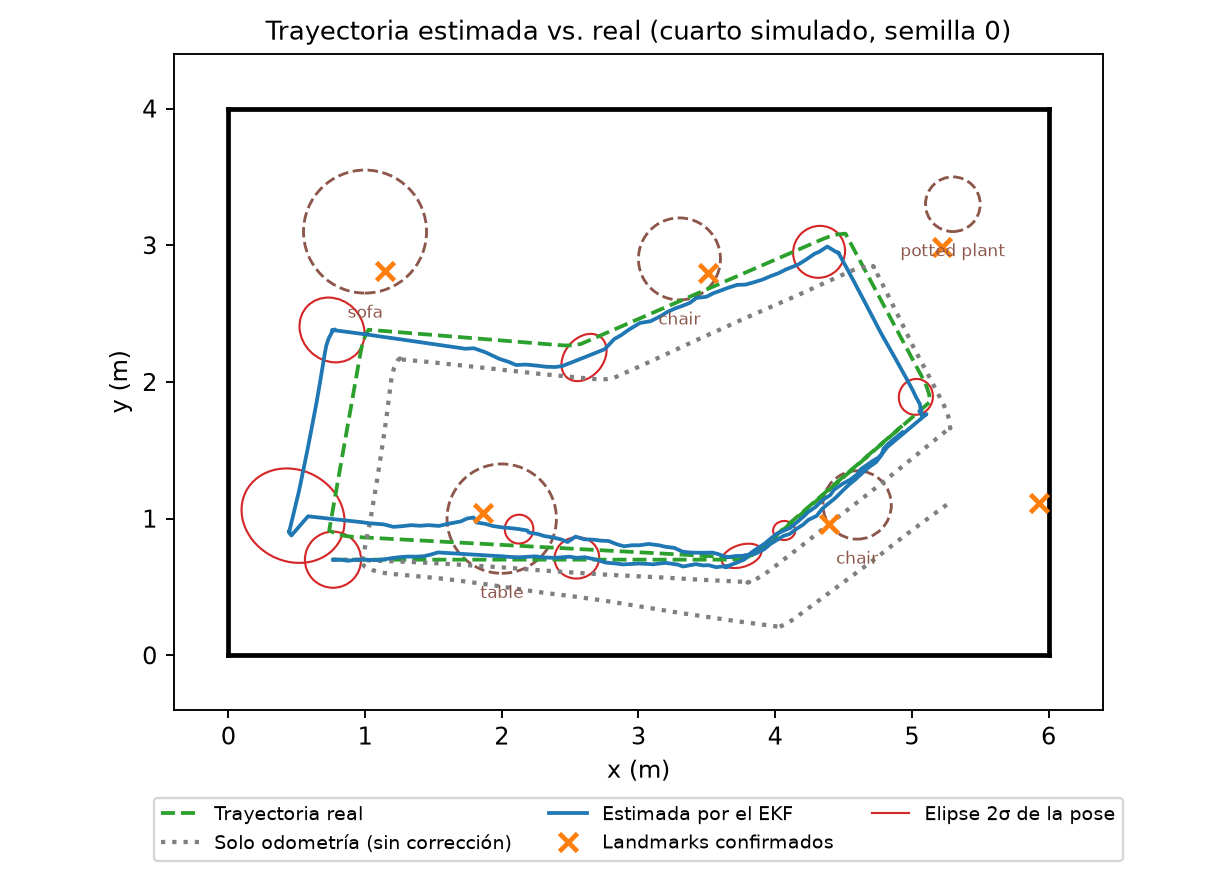
\includegraphics[width=0.85\textwidth]{Capturas_TT2/slam_trayectorias.png}
    \caption{Trayectoria real, estimada por el EKF y solo con odometría en el cuarto
    simulado. Los círculos discontinuos son los obstáculos reales.}
    \label{fig:slam_trayectorias}
\end{figure}

La Tabla~\ref{tab:slam_semillas} reporta seis corridas con semillas aleatorias
distintas.

\begin{table}[H]
\centering
\caption{Resultados del SLAM en el banco de simulación (300 ciclos por corrida)}
\label{tab:slam_semillas}
\renewcommand{\arraystretch}{1.2}
\begin{tabular}{|c|c|c|c|c|}
\hline
\textbf{Semilla} & \textbf{ATE EKF (m)} & \textbf{ATE solo odometría (m)} &
\textbf{Error de orientación} & \textbf{Landmarks} \\
\hline
0 & 0.142 & 0.318 & $2.31^\circ$ & 6 \\
1 & 0.288 & 0.250 & $4.16^\circ$ & 7 \\
2 & 0.270 & 0.273 & $3.86^\circ$ & 6 \\
3 & 0.116 & 0.191 & $2.64^\circ$ & 7 \\
4 & 0.249 & 0.164 & $1.71^\circ$ & 6 \\
5 & 0.205 & 0.188 & $2.48^\circ$ & 8 \\
\hline
\textbf{Promedio} & \textbf{0.212} & \textbf{0.231} & $\mathbf{2.86^\circ}$ & \textbf{6.7} \\
\hline
\end{tabular}
\end{table}

Estos números hay que leerlos con cuidado. En promedio el EKF baja el error de 0.23 a
0.21~m, pero no en todas las corridas, porque en dos de las seis la odometría sola fue
más precisa. En recorridos cortos y sin sesgo, como los del banco, integrar la odometría
ya da un buen resultado, y las correcciones contra \emph{landmarks} ubicados con
distancia monocular meten un error parecido al que quitan. Con una odometría real la
historia cambia, porque la longitud de paso nunca queda perfectamente calibrada y los
sensores tienen sesgo. Para ver ese caso se repitió el experimento con recorridos de
1200 ciclos (unas cuatro vueltas al cuarto) y con odometría sesgada; los resultados están
en la Tabla~\ref{tab:slam_deriva} y en la Figura~\ref{fig:slam_deriva}.

\begin{table}[H]
\centering
\caption{ATE promedio (y máximo) en seis corridas con odometría sesgada}
\label{tab:slam_deriva}
\renewcommand{\arraystretch}{1.2}
\begin{tabular}{|p{5.6cm}|c|c|}
\hline
\textbf{Escenario} & \textbf{EKF (m)} & \textbf{Solo odometría (m)} \\
\hline
300 ciclos, sin sesgo & 0.21 (0.29) & 0.23 (0.32) \\
1200 ciclos, sin sesgo & 0.28 (0.35) & 0.42 (0.61) \\
1200 ciclos, longitud de paso +10\,\% & 0.38 (0.62) & 0.58 (0.80) \\
1200 ciclos, giro sesgado $+0.1^\circ$/ciclo & 0.89 (1.68) & 1.64 (1.86) \\
1200 ciclos, ambos sesgos & 1.34 (1.89) & 1.75 (2.01) \\
\hline
\end{tabular}
\end{table}

\begin{figure}[H]
    \centering
    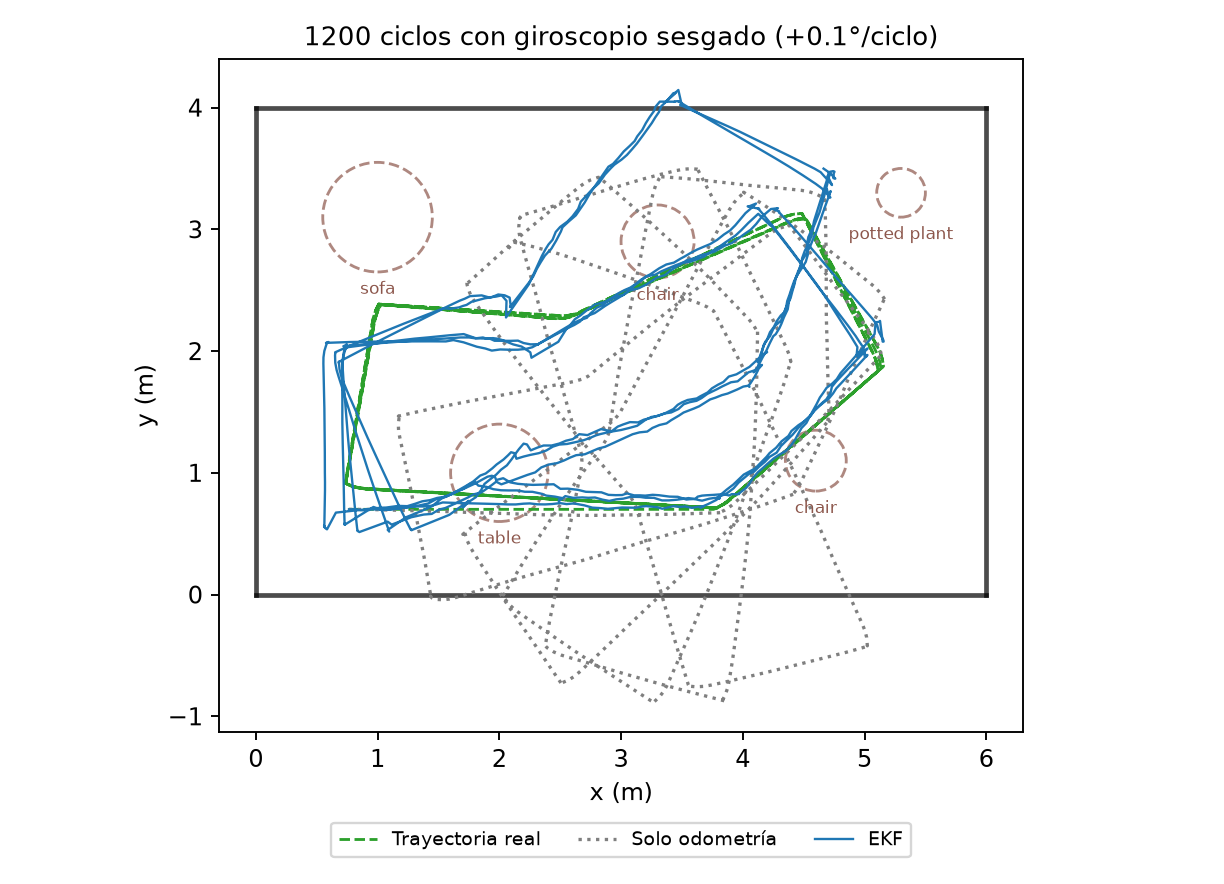
\includegraphics[width=0.78\textwidth]{Capturas_TT2/slam_deriva.png}
    \caption{Recorrido de 1200 ciclos con giroscopio sesgado (semilla 0). La odometría
    sola va girando el recorrido; el EKF lo mantiene cerca del real, aunque con
    desviaciones de hasta un metro en algunos tramos.}
    \label{fig:slam_deriva}
\end{figure}

En recorridos largos y con error de escala en el paso, el EKF reduce el error de la
odometría en alrededor de un tercio, que es justo para lo que sirve el SLAM. Con el
giroscopio sesgado lo reduce casi a la mitad en promedio, aunque el máximo llega a
1.7~m, y con los dos sesgos juntos la mejora baja a una cuarta parte. En esas corridas
se observó una divergencia de orientación, ya que en dos de las seis el error de rumbo
pasó de $100^\circ$ hacia el final. Con el rumbo tan equivocado, las detecciones dejan
de asociarse con los \emph{landmarks} que ya existen y se crean duplicados desplazados
(hasta diez sillas en un cuarto que tiene dos), y el filtro termina siendo consistente
con un mapa erróneo. Es la forma típica en que falla un EKF sin cierre de lazo.

En el prototipo este caso es poco probable, porque el giro no se integra a partir del
giroscopio sino que se toma del rumbo que entrega la BNO055 en su modo de fusión con
magnetómetro. Ese rumbo es absoluto, así que el sesgo no se va sumando como en la
simulación. Para que funcione, la brújula debe estar calibrada; por eso, al arrancar,
el sistema revisa el estado de calibración del magnetómetro y, si es bajo, le pide al
usuario que mueva los lentes en forma de ocho. El experimento sigue siendo útil por dos
razones, ya que muestra lo que pasaría con una brújula mal calibrada o alterada por
estructuras metálicas, y describe el modo de respaldo sin IMU, en el que el giro sale
del flujo óptico y sí acumula error.

\textbf{Pérdida de observaciones.} Para probar el manejo de oclusiones se repitió la
corrida de la semilla 0 quitando todas las detecciones visuales entre los ciclos 120 y
200. En la Figura~\ref{fig:slam_incertidumbre} se ve que, durante la oclusión, la traza
de la covarianza crece sin parar y la confianza cae casi a cero, es decir, el sistema se
da cuenta de que su pose ya no es fiable. En cuanto vuelve a ver objetos conocidos
(ciclo 220), la incertidumbre se reduce de golpe. El ATE de esta corrida fue de
0.08~m, así que la oclusión no hizo que el sistema se perdiera. En la corrida normal
también hay caídas de confianza en los tramos donde la cámara no tiene objetos a la
vista.

\begin{figure}[H]
    \centering
    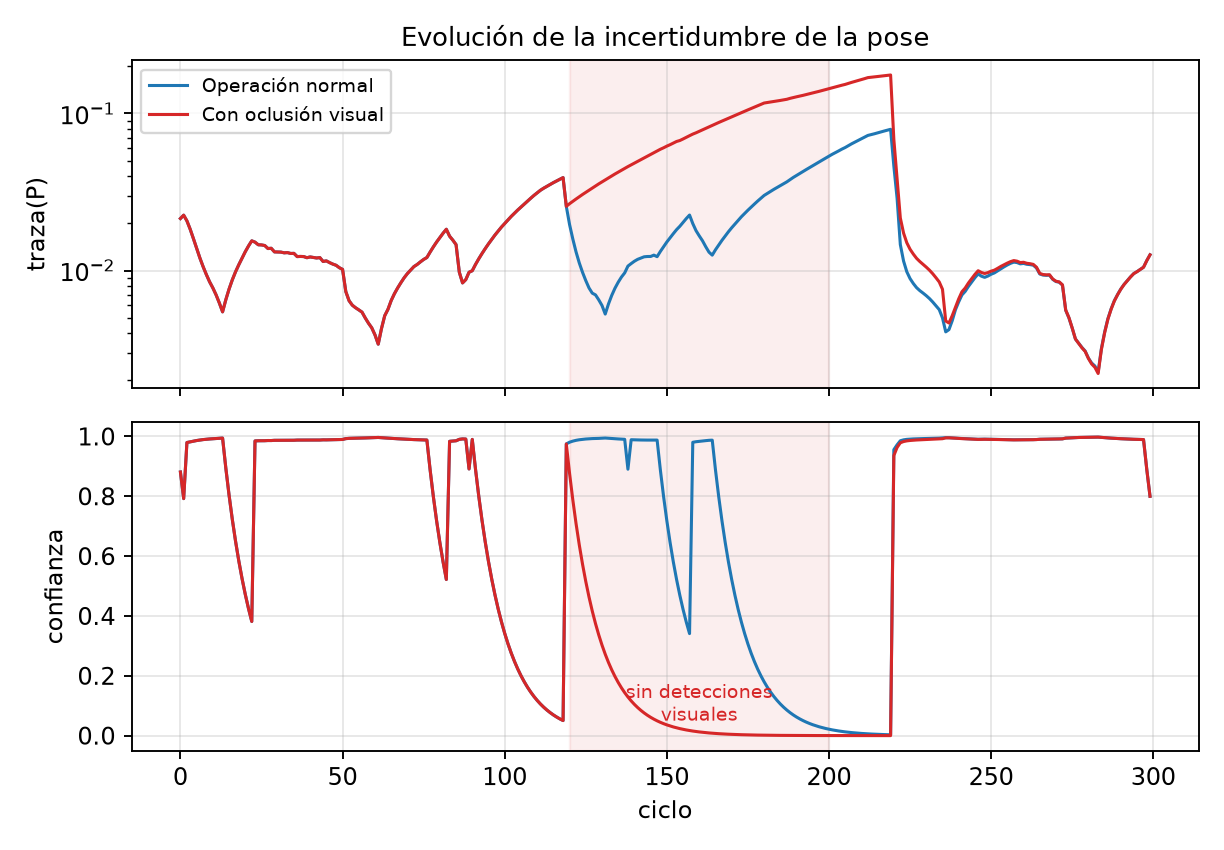
\includegraphics[width=0.85\textwidth]{Capturas_TT2/slam_incertidumbre.png}
    \caption{Evolución de la traza de la covarianza (escala logarítmica) y de la
    confianza, con y sin oclusión visual entre los ciclos 120 y 200.}
    \label{fig:slam_incertidumbre}
\end{figure}

Al quitar al azar el 60\,\% de las detecciones visuales en las seis corridas, el ATE
promedio fue de 0.23~m (máximo 0.28~m), por lo que el módulo aguanta bien las
detecciones intermitentes.

\textbf{Videos reales.} En los 19 videos grabados, el SLAM confirmó entre 1 y 39
\emph{landmarks} por recorrido. En interiores la clase más frecuente fue la puerta,
con entre 9 y 17 por recorrido de oficina. En las calles hubo muy pocos objetos
estáticos de las clases que se detectan, y en el recorrido más pobre se confirmó uno
solo, de modo que el sistema avanzó casi todo el tiempo con la pura predicción. La
Sección~\ref{sec:dev_integracion} presenta capturas del sistema trabajando con video.

\textbf{Costo computacional.} Un ciclo del EKF tarda en promedio 0.03~ms en el banco,
con unos siete \emph{landmarks}, y 0.27~ms con video real, con unos cuarenta, porque la
asociación crece linealmente con su número. En la Raspberry Pi del prototipo el ciclo
tarda \TODO{tiempo por ciclo del EKF en la Raspberry Pi}. En cualquier caso el costo es
mínimo frente a los 100~ms por ciclo que permite RNF-03.

\subsection{Limitaciones}

El rumbo absoluto de la BNO055 depende de que el magnetómetro esté calibrado y de que no
haya perturbaciones magnéticas cerca, como estructuras de acero o equipos eléctricos. La
calibración se revisa al arrancar, pero durante la sesión ningún módulo reacciona si
empeora. \TODO{avisar al usuario si la calibración del magnetómetro baja durante la
sesión}.

El filtro no hace cierre de lazo (\emph{loop closure}). Si la deriva es grande al
regresar a una zona ya visitada, el error no se reparte a lo largo de la trayectoria
anterior, y si el error de orientación rebasa lo que tolera la compuerta de asociación,
aparecen \emph{landmarks} duplicados y el filtro puede divergir. La posición de los
\emph{landmarks} monoculares depende además de la altura típica de su clase, así que un
objeto de tamaño poco común puede quedar mal ubicado, como el que aparece junto a la
pared en la Figura~\ref{fig:slam_trayectorias}. La asociación por vecino más cercano
también puede confundir dos objetos cercanos de la misma clase; una prueba de
compatibilidad conjunta \cite{neira2001jcbb} sería más confiable, a cambio de más
cómputo.

Por último, los valores de ruido de la odometría se ajustaron en simulación.
\TODO{medir el ruido real de la IMU y del conteo de pasos en el prototipo y actualizar
los parámetros del filtro}. En los mapas que se obtienen de video la escala depende de
la velocidad de caminata supuesta, porque el video no trae información de
desplazamiento.


% ==============================================================================
\section{Módulo de Ray Casting}
\label{sec:dev_ray}
% ==============================================================================

\subsection{Descripción}

El módulo de Ray Casting, implementado en \texttt{occupancy\_grid.py}, es el puente
entre las observaciones del SLAM y el mapa de ocupación. En el sistema final cumple
dos funciones distintas que comparten el mismo núcleo de recorrido de celdas:

\begin{enumerate}
    \item \textbf{Actualización del mapa.} Desde la pose estimada se traza un rayo por
    cada observación; las celdas atravesadas acumulan evidencia de espacio libre y la
    celda del extremo acumula evidencia de ocupación. Esto corresponde al modelo
    inverso del sensor de los mapas de ocupación \cite{moravec1985sonar, elfes1989}.
    \item \textbf{Consulta del mapa.} Desde la pose actual se lanzan rayos virtuales
    sobre el mapa ya construido para medir la distancia libre en cada dirección. Estas
    distancias son las variables $d_{\text{front}}$, $d_{\text{left}}$ y
    $d_{\text{right}}$ que recibe el módulo de navegación.
\end{enumerate}

En el diseño de TT1 solo se contemplaba la primera función con la regla básica ``libre
en el recorrido, ocupado al final''. Durante el desarrollo esa regla resultó
insuficiente porque las observaciones del sistema tienen precisiones muy distintas
(5~cm del ultrasonido frente a $\pm 30$\,\% de la estimación monocular), por lo que se
añadieron las reglas descritas en esta sección.

\subsection{Discretización y recorrido de celdas}

El plano se discretiza en celdas de $5 \times 5$~cm. Un punto $(x, y)$ del mundo
corresponde a la celda $(\lfloor x / 0.05 \rfloor,\; \lfloor y / 0.05 \rfloor)$, y el
extremo de un rayo con rango $r$ y dirección relativa $\phi$ desde la pose
$(x, y, \theta)$ es:

\[
x_e = x + r\cos(\theta + \phi),
\qquad
y_e = y + r\sin(\theta + \phi)
\]

Las celdas atravesadas entre la celda del usuario y la del extremo se obtienen con el
algoritmo de Bresenham \cite{bresenham1965}, que avanza celda por celda utilizando
únicamente sumas y comparaciones de enteros (Figura~\ref{fig:ray_bresenham}). Para un
alcance máximo de 4~m, un rayo recorre a lo sumo 80 celdas. Se consideró el algoritmo
de recorrido de vóxeles de Amanatides y Woo \cite{amanatides1987voxel}, que visita
todas las celdas que toca el segmento, pero Bresenham resultó suficiente para la
actualización y es más sencillo; la consecuencia de esta elección en la consulta se
discute en las limitaciones.

\begin{figure}[H]
    \centering
    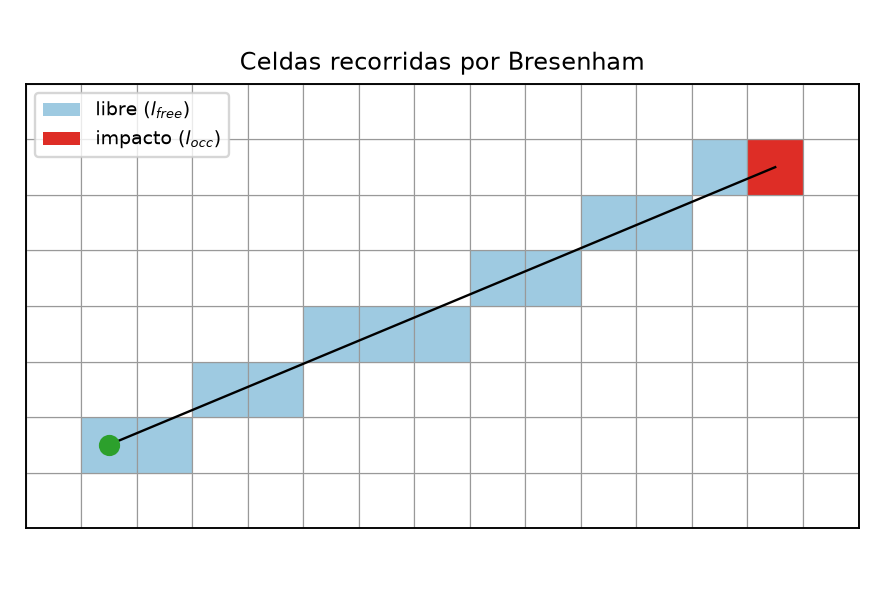
\includegraphics[width=0.6\textwidth]{Capturas_TT2/raycasting_bresenham.png}
    \caption{Celdas recorridas por el algoritmo de Bresenham para un rayo: las celdas
    intermedias reciben evidencia de espacio libre y la celda del extremo, de
    ocupación.}
    \label{fig:ray_bresenham}
\end{figure}

\subsection{Modelo inverso del sensor en log-odds}

Cada celda almacena el logaritmo de la razón de probabilidades de estar ocupada,
$l = \log\frac{p}{1-p}$, de modo que la fusión de una nueva observación es una suma
\cite{thrun2005probabilistic}. La probabilidad se recupera como
$p = 1/(1 + e^{-l})$. La Tabla~\ref{tab:ray_constantes} resume las constantes
utilizadas.

\begin{table}[H]
\centering
\caption{Constantes del modelo inverso del sensor}
\label{tab:ray_constantes}
\renewcommand{\arraystretch}{1.25}
\begin{tabular}{|p{2.6cm}|c|c|p{6.8cm}|}
\hline
\textbf{Constante} & \textbf{Log-odds} & \textbf{Probabilidad} & \textbf{Significado} \\
\hline
$l_{occ}$ & $+1.2$ & 0.77 & Incremento en la celda donde termina un rayo preciso. \\
\hline
$l_{free}$ & $-0.4$ & 0.40 & Incremento en cada celda atravesada. \\
\hline
$l_{\min}, l_{\max}$ & $\pm 5.0$ & 0.007 / 0.993 & Saturación de la celda. \\
\hline
Umbral de ocupado & $1.0$ & 0.73 & Por encima, la celda se considera obstáculo. \\
\hline
$L_{block}$ & $2.0$ & 0.88 & Por encima, la celda se considera una superficie
consolidada que detiene los rayos de espacio libre. \\
\hline
\end{tabular}
\end{table}

La asimetría entre $l_{occ}$ y $l_{free}$ es intencional: un rayo atraviesa muchas
celdas pero termina en una sola, por lo que la evidencia de ocupación debe pesar más
para que los obstáculos no se borren por los rayos que pasan junto a ellos. La
saturación en $\pm 5$ evita que una celda acumule tanta evidencia que después no pueda
corregirse \cite{hornung2013octomap}. La Figura~\ref{fig:ray_logodds} muestra el
efecto con las mismas reglas del código: una celda que se vio libre muchas veces
necesita seis impactos para volver a considerarse ocupada cuando aparece un
obstáculo. La figura también muestra la limitación discutida al final de esta
sección: una vez que la celda supera $L_{block}$, los rayos de espacio libre se
detienen en ella y su valor ya no disminuye aunque el obstáculo se retire.

\begin{figure}[H]
    \centering
    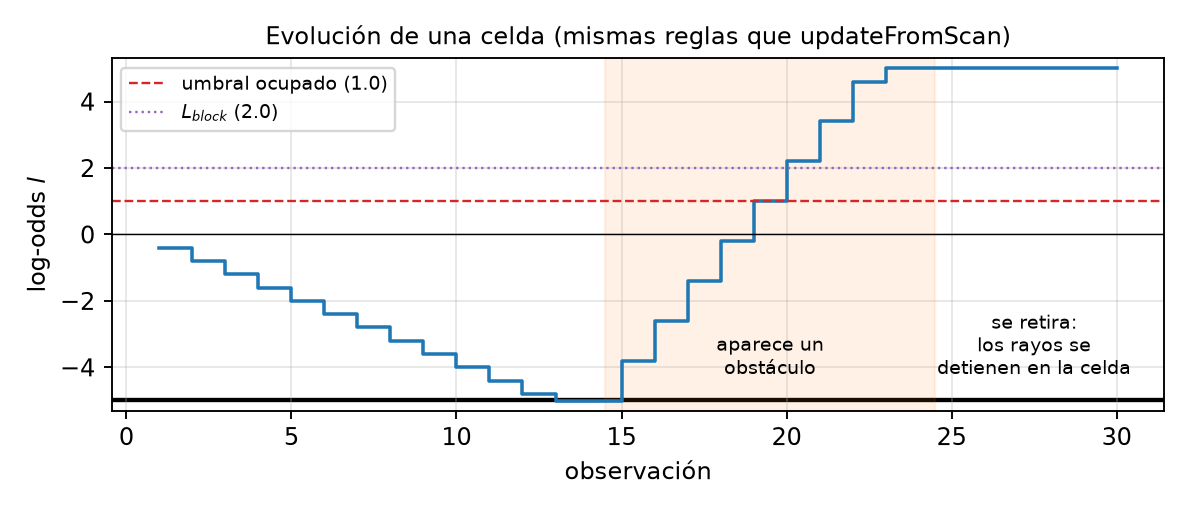
\includegraphics[width=0.82\textwidth]{Capturas_TT2/raycasting_logodds.png}
    \caption{Evolución del log-odds de una celda que primero se observa libre, después
    ocupada y finalmente queda libre otra vez, calculada con las reglas de
    \texttt{updateFromScan}.}
    \label{fig:ray_logodds}
\end{figure}

\subsection{Reglas añadidas durante el desarrollo}

Sobre el modelo básico se implementaron las siguientes reglas, cada una motivada por
un problema observado durante las pruebas:

\begin{enumerate}
    \item \textbf{El rango impreciso no marca ocupación.} Si la observación tiene
    $\sigma_r > 0.15$~m (estimación monocular cruda), el rayo solo despeja espacio
    libre hasta $r - 2\sigma_r$ y no marca la celda final como ocupada. El propósito
    es evitar que el ruido monocular deje manchas de celdas ocupadas alrededor de cada
    objeto y que despeje como libre el espacio donde realmente está el objeto. La
    ocupación de los objetos detectados por visión llega al mapa por la vía precisa:
    el rayo anclado a la posición consolidada del \emph{landmark} que genera el SLAM.
    \item \textbf{Las superficies consolidadas detienen el rayo.} Si al recorrer el
    rayo se encuentra una celda con $l > L_{block}$, el recorrido se detiene y no se
    marca nada más allá. Así un rayo ruidoso no perfora una pared ya registrada ni
    pinta marcas fantasma detrás de ella.
    \item \textbf{Rayos sin eco.} Cuando un sensor ultrasónico no recibe eco, se genera
    un rayo de espacio libre con la longitud del alcance máximo; como su extremo cae
    fuera del alcance útil, no marca ocupación. Esto permite registrar pasillos libres.
    \item \textbf{Recorte en lugar de descarte.} En la retícula de tamaño fijo, si el
    extremo de un rayo cae fuera del mapa, el rayo se recorta en el borde y se
    conservan las celdas libres recorridas. Inicialmente esos rayos se descartaban
    completos. En el mapa por bloques (Sección~\ref{sec:dev_mapeo}) esta regla deja de
    ser necesaria porque el mapa no tiene bordes.
    \item \textbf{Alcance máximo.} Los rayos se limitan a 4~m; una observación más
    lejana solo despeja espacio libre hasta ese límite.
    \item \textbf{Peligros de piso.} Las observaciones marcadas como peligro (hoyos,
    agua, escaleras) no modifican el log-odds, ya que el espacio por encima de un hoyo
    está libre; en su lugar suman un impacto en una capa separada que se describe en
    el módulo de mapeo.
\end{enumerate}

La Figura~\ref{fig:ray_casos} muestra el resultado de ejecutar el código del módulo en
tres casos representativos, con celdas de 10~cm para facilitar su lectura.

\begin{figure}[H]
    \centering
    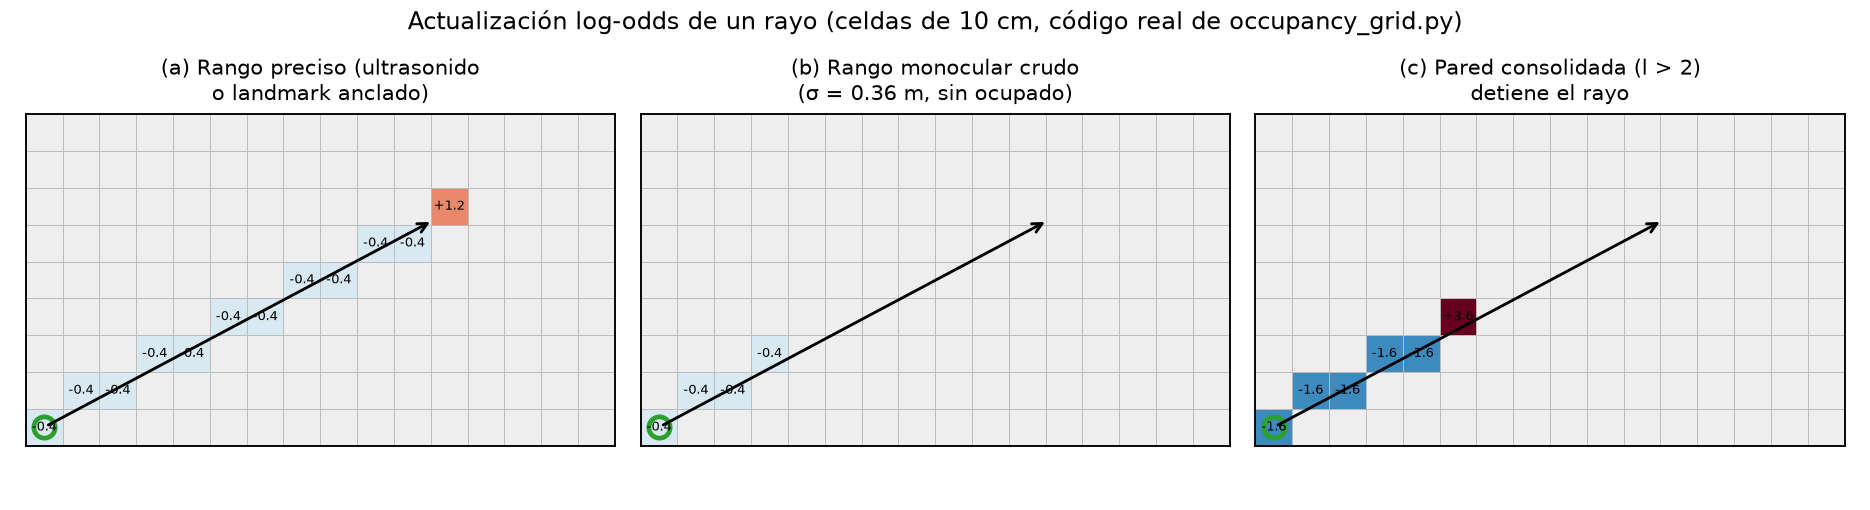
\includegraphics[width=\textwidth]{Capturas_TT2/raycasting_casos.png}
    \caption{Actualización de un rayo en tres casos: (a) rango preciso, que despeja el
    recorrido y marca el extremo; (b) rango monocular crudo, que solo despeja hasta
    $r - 2\sigma_r$; (c) rayo detenido por una superficie consolidada.}
    \label{fig:ray_casos}
\end{figure}

El Algoritmo~\ref{alg:dev_ray_update} describe la actualización tal como quedó
implementada en \texttt{updateFromScan}.

\begin{center}
\captionof{algorithm}{Actualización del mapa por Ray Casting}
\label{alg:dev_ray_update}
\end{center}
\vspace{-1.8cm}
\rule{\textwidth}{0.4pt}
\vspace{-0.9cm}
\begin{algorithmic}[1]

\Statex \textbf{ENTRADA:}
\Statex pose \Comment{(x, y, $\theta$) estimada por el SLAM}
\Statex observaciones \Comment{ancladas a landmarks + ecos + rayos sin eco}
\Statex alcance\_max \Comment{4 m}
\Statex \textbf{SALIDA:}
\Statex mapa actualizado (log-odds y capa de peligros)

\Statex
\State celda\_origen $\gets$ a\_celda(x, y)
\For{cada obs en observaciones}
    \State r $\gets$ mín(obs.r, alcance\_max)
    \State impreciso $\gets$ obs.$\sigma_r > 0.15$
    \State extremo $\gets$ a\_celda(x + r cos($\theta$ + obs.$\phi$), y + r sin($\theta$ + obs.$\phi$))
    \State celdas $\gets$ bresenham(celda\_origen, extremo)
    \State libres $\gets$ celdas sin la última
    \If{impreciso}
        \State libres $\gets$ primeras celdas hasta la distancia r $- 2\sigma_r$
    \EndIf
    \State bloqueado $\gets$ falso
    \For{cada c en libres}
        \If{l(c) $> L_{block}$}
            \State bloqueado $\gets$ verdadero;\; salir del ciclo
        \EndIf
        \State l(c) $\gets$ saturar(l(c) + $l_{free}$, $-5$, $+5$)
    \EndFor
    \If{no bloqueado Y obs.r $\leq$ alcance\_max}
        \If{obs es peligro de piso}
            \State peligros(extremo) $\gets$ mín(peligros(extremo) + 1, 10)
        \ElsIf{no impreciso}
            \State l(extremo) $\gets$ saturar(l(extremo) + $l_{occ}$, $-5$, $+5$)
        \EndIf
    \EndIf
\EndFor

\end{algorithmic}
\vspace{-0.9cm}
\rule{\textwidth}{0.4pt}

\subsection{Rayos de consulta}

La segunda función del módulo es medir el espacio libre alrededor del usuario sobre
el mapa construido. La función \texttt{castDistance} recorre con Bresenham las celdas
desde la pose en una dirección dada y devuelve la distancia al centro de la primera
celda bloqueada, entendida como una celda con $l > 1.0$ o con al menos dos impactos
en la capa de peligros; si no encuentra ninguna, devuelve el alcance máximo de 4~m.

Para construir las variables del vector de estado del módulo de navegación, la
función \texttt{directionDistances} divide el entorno del usuario en tres sectores
(Figura~\ref{fig:ray_sectores}): frente ($|\phi| \leq 30^\circ$), izquierda
($30^\circ < \phi \leq 90^\circ$) y derecha ($-90^\circ \leq \phi < -30^\circ$). En
cada sector se lanzan cinco rayos equiespaciados y se conserva la distancia mínima,
lo cual es conservador: basta con que un rayo encuentre un obstáculo para que el
sector se considere ocupado a esa distancia.

\begin{figure}[H]
    \centering
    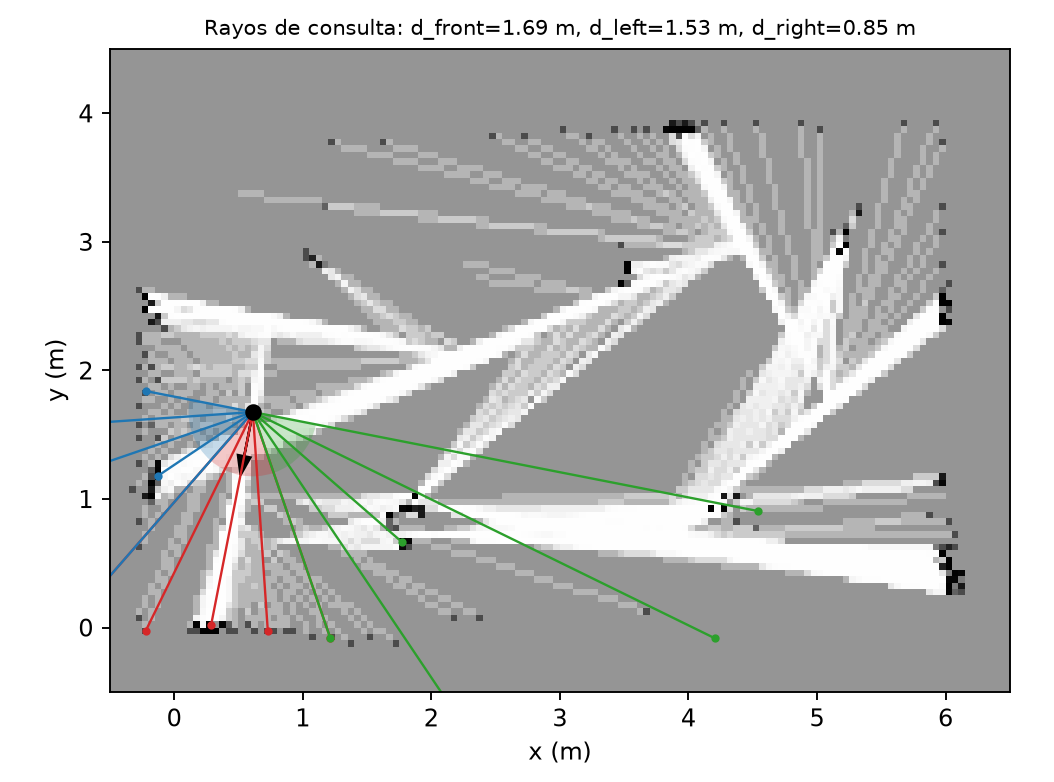
\includegraphics[width=0.75\textwidth]{Capturas_TT2/raycasting_sectores.png}
    \caption{Rayos de consulta por sector sobre el mapa construido en simulación. El
    título indica las distancias resultantes que se entregan al módulo de
    navegación.}
    \label{fig:ray_sectores}
\end{figure}

\begin{center}
\captionof{algorithm}{Distancias libres por sector}
\label{alg:dev_ray_query}
\end{center}
\vspace{-1.8cm}
\rule{\textwidth}{0.4pt}
\vspace{-0.9cm}
\begin{algorithmic}[1]

\Statex \textbf{ENTRADA:} mapa, pose (x, y, $\theta$), alcance\_max = 4 m
\Statex \textbf{SALIDA:} $d_{\text{front}}$, $d_{\text{left}}$, $d_{\text{right}}$

\Statex
\Function{castDistance}{x, y, $\alpha$}
    \For{cada c en bresenham(a\_celda(x, y), a\_celda(x + 4 cos $\alpha$, y + 4 sin $\alpha$))}
        \If{c no es la celda del usuario Y (l(c) $> 1.0$ O peligros(c) $\geq 2$)}
            \State \Return mín(4, distancia(x, y, centro(c)))
        \EndIf
    \EndFor
    \State \Return 4
\EndFunction

\Statex
\For{cada sector (a0, a1) en \{frente: ($-30^\circ$, $30^\circ$), izq: ($30^\circ$, $90^\circ$), der: ($-90^\circ$, $-30^\circ$)\}}
    \State d $\gets$ 4
    \For{k = 0 hasta 4}
        \State d $\gets$ mín(d, castDistance(x, y, $\theta$ + a0 + (a1 $-$ a0) k / 4))
    \EndFor
    \State d\_sector $\gets$ d
\EndFor
\State \Return $d_{\text{front}}$, $d_{\text{left}}$, $d_{\text{right}}$

\end{algorithmic}
\vspace{-0.9cm}
\rule{\textwidth}{0.4pt}

El módulo de navegación utiliza además una versión vectorizada con NumPy del mismo
principio para simular sensores durante el entrenamiento del agente, la cual se
documentará junto con ese módulo.

\subsection{Resultados}

En el banco de simulación, la actualización del mapa con todas las observaciones de un
ciclo (cuatro a seis rayos) tomó en promedio 0.15~ms, y en el procesamiento de video
real, incluyendo el despeje de la huella del usuario, 0.23~ms por ciclo. La
construcción completa del cuadro para navegación, que incluye los quince rayos de
consulta y el mapa local, tomó 0.51~ms. Estos tiempos son dos órdenes de magnitud
menores que el periodo de 100~ms que impone RNF-03, por lo que el Ray Casting no
representa un cuello de botella del sistema.

Para cuantificar la aportación de las reglas añadidas se realizó un experimento de
ablación en el banco de simulación, desactivándolas una por una. Además de la
precisión y la exhaustividad, se contó el número de celdas marcadas como ocupadas que
no tienen ningún obstáculo real a menos de 10~cm (celdas falsas). Los resultados se
muestran en la Tabla~\ref{tab:ray_ablacion}.

\begin{table}[H]
\centering
\caption{Ablación de las reglas del Ray Casting (promedio de seis corridas)}
\label{tab:ray_ablacion}
\renewcommand{\arraystretch}{1.2}
\begin{tabular}{|p{6.0cm}|c|c|c|c|}
\hline
\textbf{Configuración} & \textbf{Precisión} & \textbf{Exhaustividad} &
\textbf{Ocupadas} & \textbf{Falsas} \\
\hline
Vigente (todas las reglas) & 0.60 & 0.31 & 152 & 60 \\
Sin $L_{block}$ & 0.58 & 0.30 & 172 & 73 \\
Rango monocular crudo marca ocupación & 0.60 & 0.32 & 157 & 63 \\
Sin anclar a \emph{landmarks} (rango crudo) & 0.62 & 0.31 & 150 & 57 \\
Sin las tres reglas & 0.57 & 0.35 & 192 & 82 \\
\hline
\end{tabular}
\end{table}

En conjunto, las reglas reducen las celdas falsas de 82 a 60 (alrededor de 27\,\%), y
la mayor parte de esa mejora proviene de $L_{block}$. Quitar las tres reglas sube un
poco la exhaustividad, porque el mapa marca más celdas, pero a costa de más celdas
falsas. Las reglas del rango monocular y del anclaje casi no modifican las métricas
globales del banco, porque la mayoría de las celdas ocupadas corresponden a paredes
registradas por ultrasonido y los objetos son una fracción pequeña del mapa; su
efecto es local, alrededor de cada objeto, donde evitan manchas difusas y marcas
duplicadas. También se observa que cerca del 40\,\% de las celdas ocupadas no
coinciden con un obstáculo real dentro de la tolerancia de 10~cm. La causa principal
no es el Ray Casting sino el error de pose: con un ATE de 0.21~m, una pared registrada
en distintos momentos queda dibujada con un desplazamiento de varias celdas. La Sección~\ref{sec:dev_mapeo}
analiza la calidad del mapa con mayor detalle.

\subsection{Limitaciones}

\begin{itemize}
    \item \textbf{Celdas consolidadas permanentes.} La regla $L_{block}$ impide que un
    rayo de espacio libre atraviese una celda con $l > 2$, lo cual también impide que
    esa celda vuelva a disminuir. En la práctica, una celda que recibió dos o más
    impactos precisos queda marcada como ocupada de forma permanente: se verificó que
    ni cincuenta rayos posteriores que la atraviesan la liberan. Esto significa que
    un obstáculo que desaparece (por ejemplo, una caja que se retira) permanece en el
    mapa, lo cual no cumple por completo con RF-17 en el caso de desaparición de
    obstáculos. Una corrección posible es permitir que los rayos precisos, cuyo
    extremo está claramente más allá de la celda, sí reduzcan su valor.
    \item \textbf{Huecos entre celdas.} Bresenham visita una sola celda por paso, por
    lo que un rayo de consulta diagonal puede pasar entre dos celdas ocupadas que solo
    se tocan por una esquina y reportar libre un frente bloqueado. Esto es frecuente en
    mapas con ecos dispersos. El módulo de navegación lo mitiga lanzando un abanico de
    tres sub-rayos por dirección; una alternativa sería usar el recorrido de
    Amanatides y Woo en la consulta.
    \item \textbf{Mapa bidimensional.} Los rayos se trazan en el plano, por lo que
    obstáculos colgantes (ramas, letreros a la altura de la cabeza) solo se registran
    si los detecta la visión.
    \item Como el rango monocular nunca marca ocupación por sí solo, los obstáculos de
    clases que la visión no reconoce y que no producen eco ultrasónico no aparecen en
    el mapa.
\end{itemize}


% ==============================================================================
\section{Módulo de mapeo}
\label{sec:dev_mapeo}
% ==============================================================================

\subsection{Descripción}

El módulo de mapeo mantiene la representación del entorno sobre la que trabajan la
navegación y las alertas, y atiende los requerimientos RF-15, RF-16 y RF-17. El diseño
de TT1 contemplaba una sola retícula de ocupación local. La primera implementación
(\texttt{occupancy\_grid.py}) siguió ese diseño con una retícula fija de
$8 \times 8$~m, pero pronto aparecieron tres problemas. El usuario puede salir de un
área de ocho metros en pocos segundos; una retícula más grande gastaría memoria aunque
casi toda quedara vacía; y el mapa se perdía al apagar el dispositivo. Para resolverlos
se desarrolló el gestor de mapa por bloques (\texttt{map\_manager.py}), que conserva la
misma interfaz de consulta de la retícula original, así que el resto del sistema no tuvo
que cambiar.

\subsection{Mapa global por bloques}

El plano se divide en bloques cuadrados fijos (\emph{chunks}) de $8 \times 8$~m,
anclados al marco de referencia del SLAM. Con celdas de 5~cm, cada bloque tiene
$160 \times 160$ celdas. Los bloques se identifican con un par de índices enteros
$(i, j)$, que pueden ser negativos, y se crean solo cuando un rayo o el propio usuario
llegan a ellos, de modo que el mapa crece únicamente hacia donde se camina. Un punto del
mundo se convierte a su bloque y a su celda local así.

\[
(g_x, g_y) = \left(\left\lfloor \frac{x}{0.05} \right\rfloor,
                   \left\lfloor \frac{y}{0.05} \right\rfloor\right),
\qquad
(i, j) = \left(\left\lfloor \frac{g_x}{160} \right\rfloor,
               \left\lfloor \frac{g_y}{160} \right\rfloor\right),
\qquad
(l_x, l_y) = (g_x - 160\,i,\; g_y - 160\,j)
\]

La idea se parece a los submapas de sistemas como Cartographer
\cite{hess2016cartographer}, con la diferencia de que aquí los bloques tienen una
posición fija en el mundo y no se reacomodan por optimización. Eso mantiene el costo
bajo, a cambio de no corregir la deriva acumulada.

Cada bloque (\texttt{MapChunk}) guarda una matriz de log-odds en punto flotante de
32 bits, que ocupa 100~KB en memoria, y una matriz de impactos de peligros de piso en
enteros de 8 bits, de 25~KB. Guarda también la etiqueta del cuarto al que pertenece, el
número de visitas, las fechas de creación y de última visita, y una bandera que indica
si tiene cambios sin guardar.

Para no llenar la memoria de la Raspberry Pi, se mantienen como máximo 25 bloques
cargados. Si se pasa de ese número, los bloques más alejados del actual (en distancia de
Chebyshev) se guardan en disco y se descargan, y si se vuelven a necesitar se cargan de
nuevo sin que el resto del sistema lo note. Los rayos cruzan de un bloque a otro sin
cortes, porque cada celda se resuelve a su bloque en el momento de leerla o escribirla,
con un pequeño caché del último bloque consultado.

\subsection{Persistencia y re-localización}

Cada mapa se guarda en una carpeta con la siguiente estructura.

\begin{verbatim}
maps/<nombre>/
    chunk_0_0.npz      log-odds (float16) + peligros + metadatos del bloque
    chunk_0_-1.npz     ...
    meta.json          resolución, tamaño de bloque, cuartos etiquetados
    landmarks.json     landmarks confirmados del SLAM (posición, etiqueta,
                       número de avistamientos)
\end{verbatim}

Los bloques se guardan comprimidos y con el log-odds en 16 bits, así que en los mapas
reales ocupan entre 1 y 7~KB cada uno y el recorrido más grande (13 bloques y
26 \emph{landmarks}) ocupa unos 60~KB. Al abrir un mapa se revisa que su resolución y
tamaño de bloque coincidan con la configuración actual, para no mezclar geometrías
distintas. Cuando el sistema arranca en un lugar ya mapeado, se restauran los bloques y
los \emph{landmarks}, y estos últimos se cargan en el SLAM para que el filtro pueda
corregir la pose contra objetos conocidos desde el primer ciclo.

El SLAM siempre arranca en el origen de su propio marco de referencia, así que la
re-localización funciona cuando el usuario empieza la sesión en el mismo punto y mirando
hacia el mismo lado que cuando se creó el mapa, por ejemplo en la entrada de su casa u
oficina. Una primera versión anunciaba como ``zona conocida'' cualquier bloque guardado
aunque el usuario estuviera en otro lugar. Ahora, mientras la re-localización está
pendiente, todos los bloques se reportan como nuevos y no se adoptan las etiquetas de
cuarto; se da por confirmada cuando el EKF acumula tres correcciones contra los
\emph{landmarks} cargados, y en ese momento el sistema lo dice en voz alta.

\subsection{Eventos de cambio de zona}

En cada ciclo el gestor recibe la pose y genera eventos que la interacción puede
anunciar por voz. El evento \texttt{chunk\_change} indica que el usuario entró a otro
bloque y si esa zona ya era conocida o es nueva. El evento \texttt{door\_crossed} se
dispara cuando el usuario pasa a menos de 0.7~m de un \emph{landmark} confirmado de tipo
puerta, lo cual se interpreta como el paso a otro cuarto, con una espera de 60 ciclos
para no repetirlo. Y \texttt{room\_recognized} indica que el bloque al que entró el
usuario tiene una etiqueta de cuarto guardada, como ``cocina''. Los cuartos se numeran
solos al cruzar puertas y se pueden renombrar con una etiqueta propia, que queda en
\texttt{meta.json}.

\subsection{Despeje de la huella del usuario}

Al procesar los videos se vio que, en pasillos sin objetos de las clases que reconoce la
visión, el mapa no registraba espacio libre, porque sin ultrasonido no había rayos que lo
despejaran, y la navegación no encontraba por dónde avanzar. Como el usuario sí pasó por
ahí, en cada ciclo se marca como libre un disco de 0.45~m de radio alrededor de su
posición (\texttt{clearFootprint}). Las celdas que ya superan el umbral de ocupación no
se tocan, para no borrar obstáculos reales.

\subsection{Capa de peligros de piso}

Un hoyo, una coladera, un charco o una escalera hacia abajo no devuelven eco ni detienen
un rayo, porque el espacio de arriba está libre, y aun así no se pueden pisar. Por eso
van en una capa separada del log-odds, siguiendo la idea de los mapas de costo por capas
\cite{lu2014layered}. Las detecciones vienen de la segmentación del módulo de visión
(SegFormer entrenado en ADE20K \cite{xie2021segformer, zhou2017ade20k}) y su distancia se
calcula por proyección al plano del piso. Cada avistamiento suma un impacto a su celda, y
la celda cuenta como peligrosa a partir de dos impactos, así que un parpadeo de la
segmentación no inventa un hoyo. En las consultas, una celda peligrosa se trata como
bloqueada y la navegación la rodea igual que a una pared.

Los impactos también pueden bajar. En cada cuadro, el módulo de visión revisa nueve
columnas de la máscara de piso transitable y, para cada una, mide hasta dónde llega el
piso sin interrupción; con eso arma unos rayos de ``piso libre'' que entrega al mapa
(\texttt{tomarPisoLibre}). Estos rayos no tocan el log-odds, solo le restan un impacto a
cada celda de peligro que cruzan. Así, si la segmentación confundió una mancha con un
hoyo y después la misma zona se ve como piso, el falso peligro se borra en pocos
cuadros. Como su distancia viene de la proyección al piso, se tratan como rango
impreciso y solo recorren la parte cercana del tramo, de modo que no borran un hoyo real
que esté justo donde termina el piso visible.

\subsection{Salida hacia el módulo de navegación}

En cada ciclo, la función \texttt{buildNavigationFrame} junta en una sola estructura, el
cuadro de navegación, todo lo que necesita el módulo de navegación. Sus campos se
describen en la Tabla~\ref{tab:nav_frame}.

\begin{table}[H]
\centering
\caption{Contenido del cuadro de navegación generado por el módulo de mapeo}
\label{tab:nav_frame}
\renewcommand{\arraystretch}{1.25}
\begin{tabular}{|p{4.2cm}|p{10.3cm}|}
\hline
\textbf{Campo} & \textbf{Descripción} \\
\hline
Salida del SLAM & Pose, covarianza, confianza y marca de tiempo. \\
\hline
Mapa local & Parche centrado en el usuario de $4 \times 4$~m ($81 \times 81$ celdas)
con dos canales, la probabilidad de ocupación y los peligros de piso. Las celdas
desconocidas valen 0.5 en el primer canal. \\
\hline
$d_{\text{front}}$, $d_{\text{left}}$, $d_{\text{right}}$ & Distancia libre por sector,
obtenida con los rayos de consulta (Sección~\ref{sec:dev_ray}). \\
\hline
$r_{\text{front}}$, $r_{\text{left}}$, $r_{\text{right}}$ & Nivel de riesgo de 0 a 3
por sector, según la tabla de riesgo de TT1, calculado con las detecciones del ciclo a
menos de 3~m. \\
\hline
Lecturas ultrasónicas & Lecturas de los dos MB1232 ya validadas y sin ecos de piso. \\
\hline
Detecciones y \emph{landmarks} & Detecciones del ciclo y \emph{landmarks}
etiquetados del mapa, que sirven para resolver destinos como ``la salida''. \\
\hline
Bloque y cuarto & Índice del bloque actual y etiqueta del cuarto, si la hay. \\
\hline
\end{tabular}
\end{table}

La Figura~\ref{fig:mapeo_costmap} muestra un ejemplo del mapa local. Para que se viera
el segundo canal, en esta figura se agregó a mano un peligro de piso de
$25 \times 25$~cm delante del usuario.

\begin{figure}[H]
    \centering
    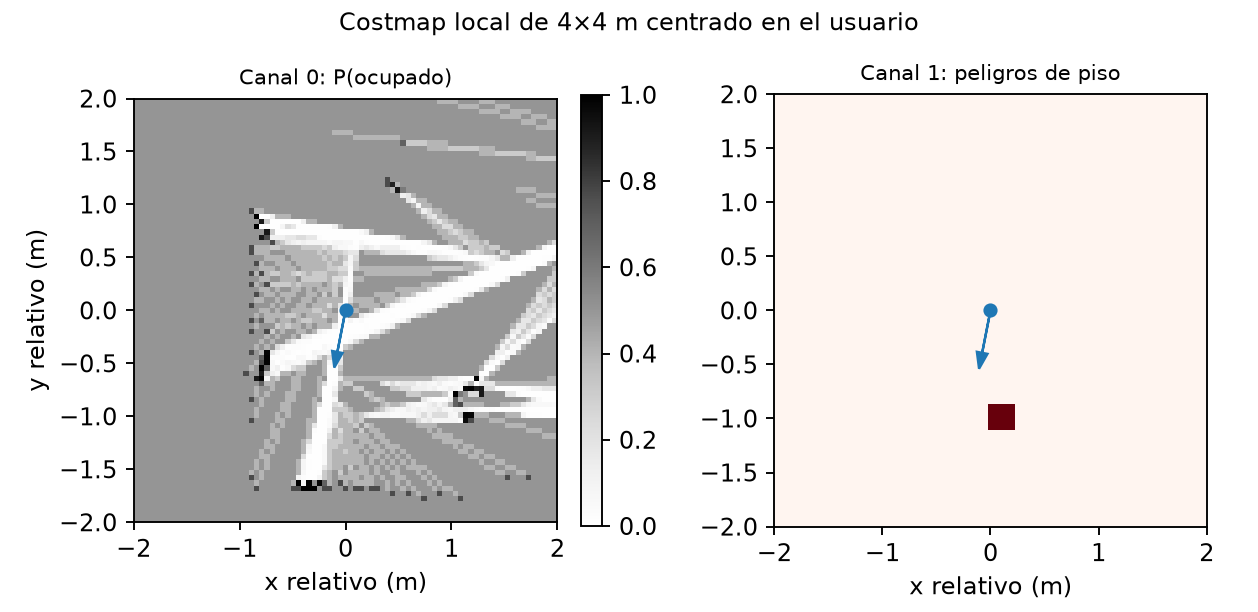
\includegraphics[width=0.85\textwidth]{Capturas_TT2/mapeo_costmap.png}
    \caption{Mapa local de $4 \times 4$~m centrado en el usuario, con la probabilidad de
    ocupación (izquierda) y los peligros de piso (derecha).}
    \label{fig:mapeo_costmap}
\end{figure}

\subsection{Del video al mapa}

Para tener mapas de muchos lugares reales sin recorrerlos todos con el prototipo se
desarrolló el script \texttt{video\_a\_mapa.py}. El script procesa videos grabados en
primera persona con el mismo flujo del sistema (visión, SLAM, Ray Casting y mapa por
bloques) y guarda el resultado. Al final genera un reporte que dice si el mapa tiene
suficiente espacio libre para usarse en el entrenamiento de la navegación y, si no,
sugiere grabar más pasadas por el mismo lugar. También trae recomendaciones de grabación,
como sostener el teléfono a la altura del pecho, caminar y girar despacio porque el giro
se estima con flujo óptico, evitar contraluces y pasar dos o más veces por cada zona
para que los \emph{landmarks} se confirmen.

\subsection{Resultados}

\textbf{Mapas con el prototipo.} \TODO{mapas construidos con el prototipo en recorridos
reales (figura y tabla con bloques, \emph{landmarks}, puertas y superficie libre), y
comparación con un plano o croquis del lugar}.

\textbf{Construcción incremental.} La Figura~\ref{fig:mapeo_evolucion} muestra cómo
evoluciona el mapa del cuarto simulado. El mapa se construye sin información previa
(RF-15); al principio solo se conocen las zonas que alcanzaron los primeros rayos y, al
terminar el recorrido, ya se distinguen el espacio libre, los obstáculos y las paredes
hacia las que el usuario caminó (RF-16). Como los dos ultrasónicos miran al frente con un
haz angosto, las paredes que solo quedan a los costados del recorrido casi no se
registran y buena parte del contorno del cuarto se queda en gris, es decir, sin conocer.

\begin{figure}[H]
    \centering
    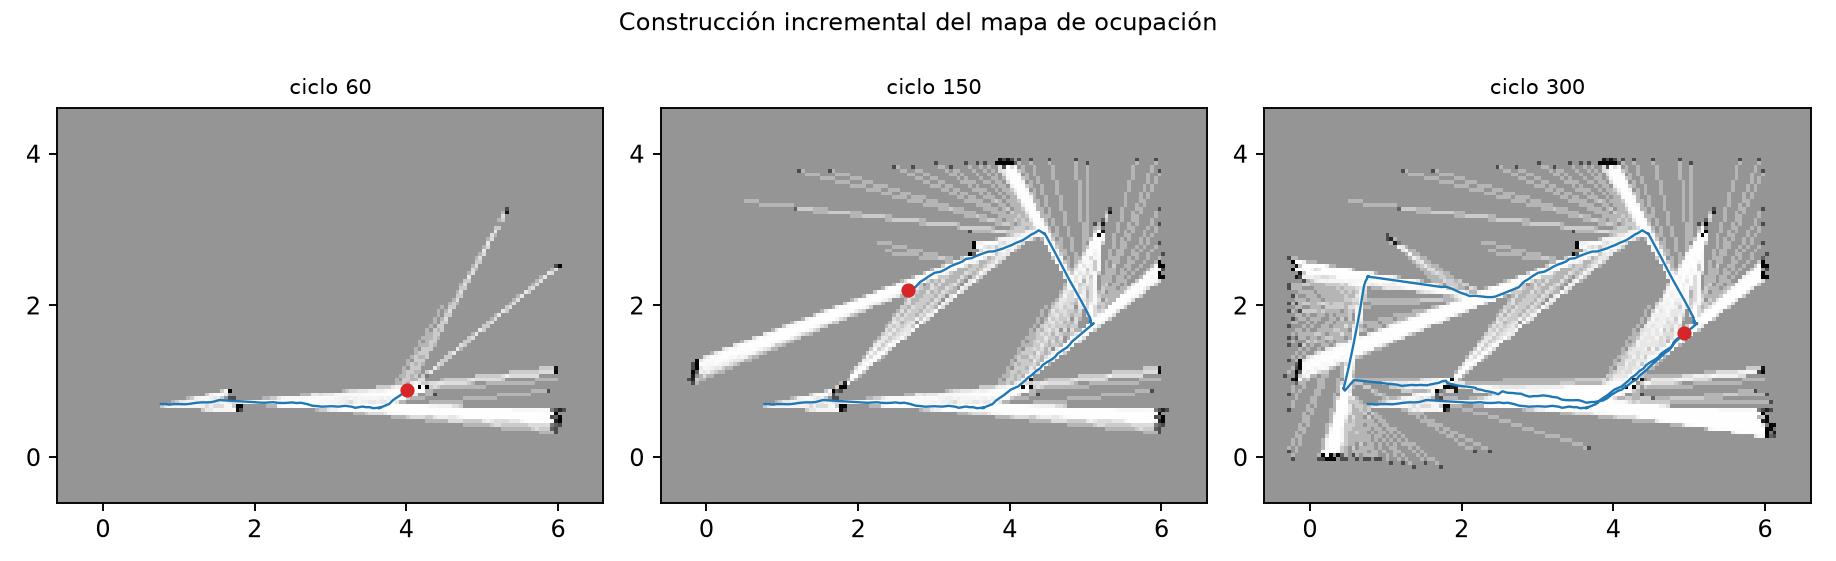
\includegraphics[width=\textwidth]{Capturas_TT2/mapeo_evolucion.png}
    \caption{Mapa de ocupación del cuarto simulado en los ciclos 60, 150 y 300. En blanco
    lo libre, en negro lo ocupado y en gris lo desconocido; la línea azul es la
    trayectoria estimada.}
    \label{fig:mapeo_evolucion}
\end{figure}

\textbf{Aporte del ultrasonido.} El banco de simulación usa el mismo montaje que el
prototipo, con dos sensores frontales paralelos separados 10~cm. Para ver qué tan buena
fue esa decisión se comparó contra otras dos disposiciones y contra el caso sin
ultrasonido (Tabla~\ref{tab:mapeo_us}). La configuración de tres sensores es la que usaba
el banco en una versión anterior, y la de sensores laterales es la que sugería la
descripción electrónica de TT1.

\begin{table}[H]
\centering
\caption{Efecto de la configuración ultrasónica (promedio de seis corridas)}
\label{tab:mapeo_us}
\renewcommand{\arraystretch}{1.2}
\begin{tabular}{|p{6.2cm}|c|c|c|}
\hline
\textbf{Configuración} & \textbf{ATE (m)} & \textbf{Precisión} &
\textbf{Exhaustividad} \\
\hline
Dos sensores frontales, como el prototipo & 0.21 & 0.60 & 0.31 \\
Tres sensores ($0^\circ$, $\pm 40^\circ$) & 0.27 & 0.48 & 0.43 \\
Dos sensores laterales ($\pm 90^\circ$) & 0.28 & 0.55 & 0.48 \\
Sin ultrasonido & 0.30 & 0.60 & 0.05 \\
\hline
\end{tabular}
\end{table}

El montaje del prototipo da la mejor localización (0.21~m) y la mejor precisión del mapa,
porque los ecos frontales coinciden con lo que ve la cámara y las paredes quedan bien
ubicadas. A cambio, registra menos superficie que las configuraciones con sensores
abiertos hacia los lados, con una exhaustividad de 0.31 contra 0.43 a 0.48. Sin
ultrasonido la exhaustividad se desploma a 0.05, porque el mapa solo registra los objetos
anclados a \emph{landmarks} y casi ninguna pared, y su precisión es alta nada más porque
marca muy pocas celdas. El resultado justifica los MB1232 sobre todo por el mapa. Abrir
un poco cada sensor hacia afuera, algo que \texttt{montaje.py} ya permite, podría
recuperar parte de la cobertura lateral, aunque se perdería el traslape central que hace
posible el cálculo estéreo del lado.

\textbf{Mapas de recorridos en video.} La Tabla~\ref{tab:mapeo_reales} resume los mapas
de los 19 videos, y las Figuras~\ref{fig:mapeo_real_pasillo} a
\ref{fig:mapeo_real_banqueta} muestran tres de ellos. Los videos no traen ultrasonido,
así que el espacio libre sale sobre todo de la huella del usuario y las celdas ocupadas
solo de los objetos anclados a \emph{landmarks}.

\begin{table}[H]
\centering
\caption{Mapas generados a partir de videos reales}
\label{tab:mapeo_reales}
\renewcommand{\arraystretch}{1.2}
\begin{tabular}{|l|c|c|c|c|c|}
\hline
\textbf{Recorrido} & \textbf{Bloques} & \textbf{Landmarks} & \textbf{Puertas} &
\textbf{Peligros} & \textbf{Libre observado (m$^2$)} \\
\hline
Calle 1 & 5 & 1 & 0 & 0 & 12.4 \\
Calle 2 & 5 & 5 & 0 & 1 & 10.6 \\
Casa & 6 & 29 & 5 & 11 & 34.5 \\
Pasillo & 9 & 25 & 13 & 1 & 45.4 \\
Plaza comercial & 13 & 26 & 6 & 4 & 38.5 \\
Oficina 1 & 8 & 23 & 11 & 1 & 19.3 \\
Oficina 2 & 4 & 12 & 9 & 0 & 20.4 \\
Video vertical & 5 & 8 & 1 & 5 & 12.7 \\
Oficina 3 & 8 & 28 & 12 & 2 & 16.9 \\
Oficina 4 & 5 & 39 & 17 & 3 & 18.3 \\
Puesto callejero & 4 & 5 & 0 & 2 & 4.2 \\
Banqueta 1 & 5 & 9 & 0 & 8 & 8.1 \\
Avenida 1 & 7 & 8 & 0 & 4 & 13.3 \\
Avenida 2 & 7 & 11 & 0 & 4 & 16.1 \\
Banqueta 2 & 8 & 16 & 0 & 13 & 37.5 \\
Esquina & 5 & 14 & 0 & 7 & 14.0 \\
Sala de maestros 1 & 4 & 4 & 2 & 0 & 1.1 \\
Sala de maestros 2 & 4 & 6 & 5 & 0 & 4.2 \\
Sala de maestros 3 & 4 & 9 & 3 & 0 & 11.5 \\
\hline
\end{tabular}
\end{table}

\begin{figure}[H]
    \centering
    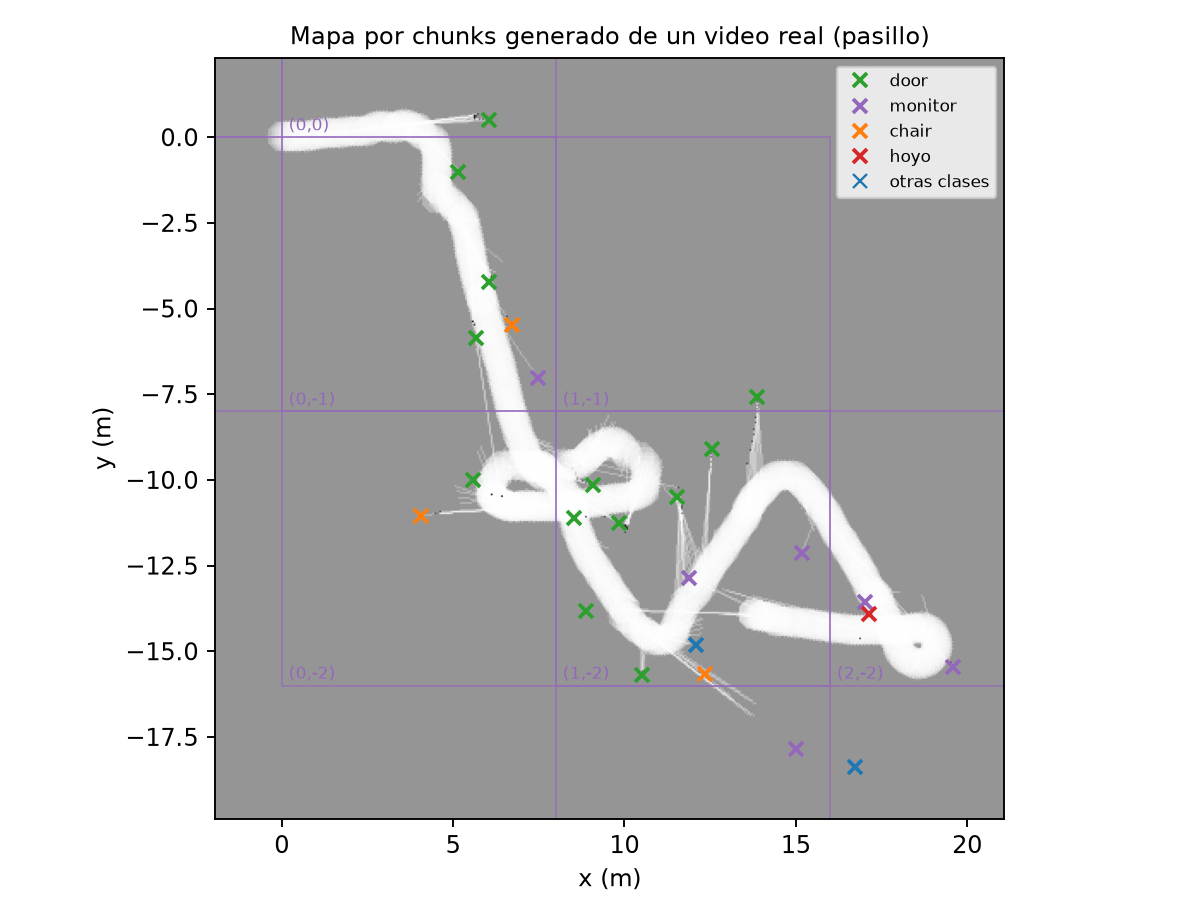
\includegraphics[width=0.8\textwidth]{Capturas_TT2/mapeo_real_pasillo.png}
    \caption{Mapa por bloques del recorrido de un pasillo. Los recuadros morados son los
    bloques de $8 \times 8$~m y las cruces, los \emph{landmarks} por clase.}
    \label{fig:mapeo_real_pasillo}
\end{figure}

\begin{figure}[H]
    \centering
    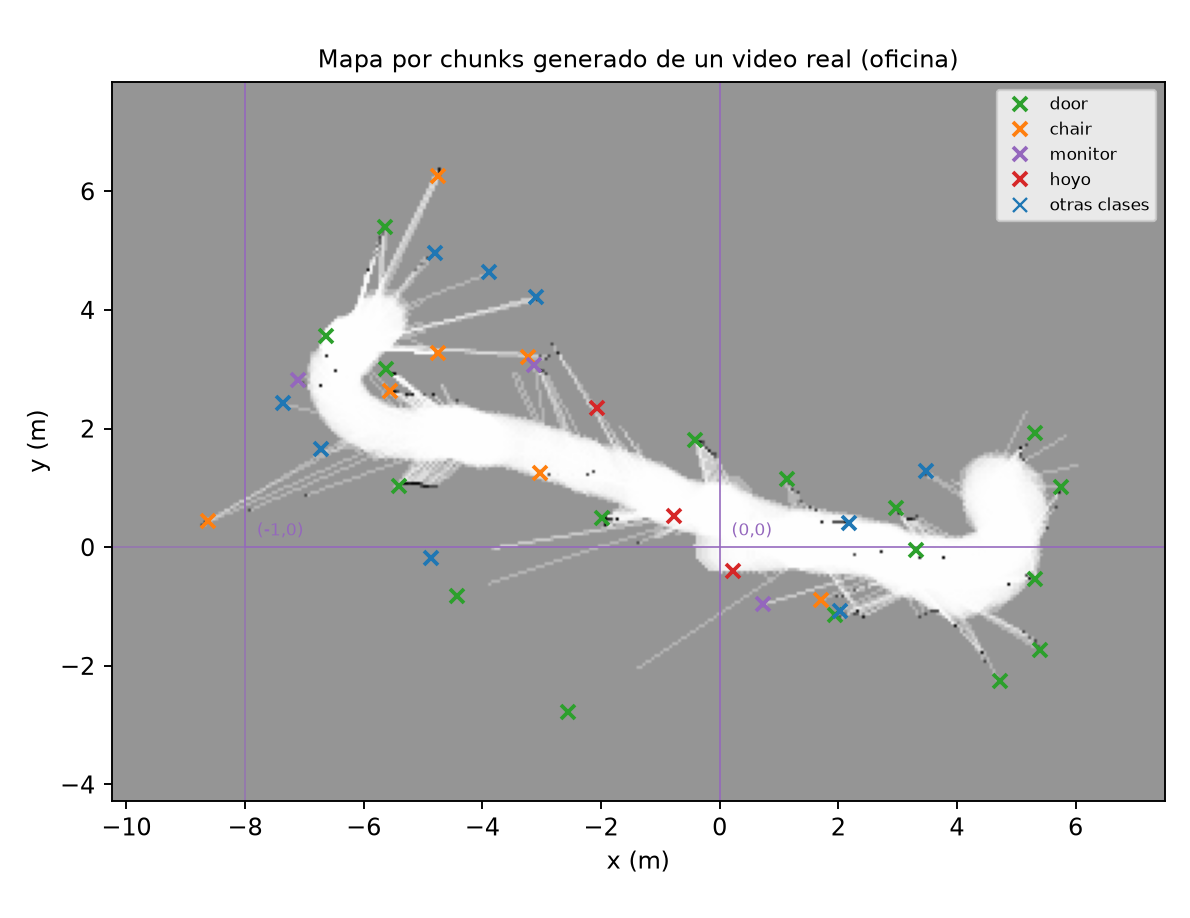
\includegraphics[width=0.8\textwidth]{Capturas_TT2/mapeo_real_oficina.png}
    \caption{Mapa por bloques del recorrido de una oficina.}
    \label{fig:mapeo_real_oficina}
\end{figure}

\begin{figure}[H]
    \centering
    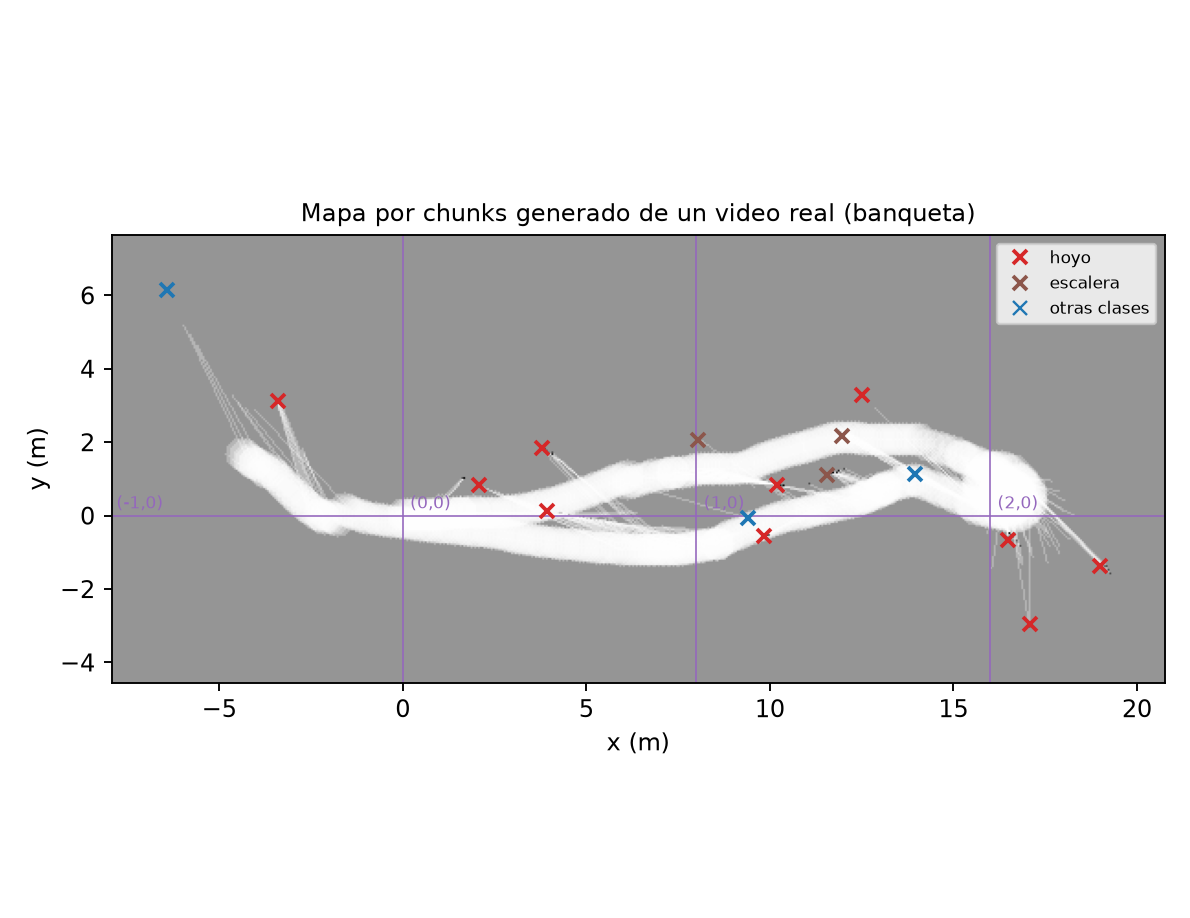
\includegraphics[width=0.8\textwidth]{Capturas_TT2/mapeo_real_banqueta.png}
    \caption{Mapa por bloques del recorrido de una banqueta, con muchos peligros de piso
    registrados.}
    \label{fig:mapeo_real_banqueta}
\end{figure}

En los recorridos de interiores las puertas son la clase más frecuente, lo cual viene
bien porque son los destinos naturales de la navegación (``llévame a la salida''). La
tabla también deja ver falsos positivos, ya que en las oficinas aparecen peligros de piso
que no son hoyos reales, probablemente porque la segmentación confunde reflejos o
cambios de textura del piso con zonas no transitables. Los mapas de calle tienen pocos
\emph{landmarks}, porque hay pocos objetos estáticos de las clases detectables, y en
cambio juntan muchos peligros de piso. En las banquetas, esos peligros pueden ser
escalones y desniveles reales que la segmentación toma por escaleras, o grietas y
manchas del pavimento; con estos datos no hay forma de separarlos.

\textbf{Persistencia.} Los 19 mapas se cargan desde disco con sus bloques,
\emph{landmarks} y valores de log-odds, y se consultan con la misma interfaz que un mapa
en memoria. Las pruebas automatizadas comprueban además que, al guardar y volver a cargar
un mapa, se conservan las celdas ocupadas, los peligros y las etiquetas de cuarto, que los
\emph{landmarks} vuelven al SLAM, que un mapa con geometría distinta se rechaza y que
descargar bloques por falta de memoria no pierde información.

\subsection{Limitaciones}

Los bloques están fijos en el mundo y no se corrigen cuando el SLAM acumula deriva, así
que un error de pose se queda ``congelado'' en el mapa. La re-localización entre
sesiones, por su parte, requiere empezar en el mismo punto y con la misma orientación
con que se creó el mapa. Los peligros de piso solo se borran cuando la cámara vuelve a
ver la zona como piso, así que un falso hoyo que quedó atrás del usuario permanece en el
mapa hasta que regrese por ahí. Los mapas de recorridos en video de la tabla anterior se
construyeron antes de agregar los rayos de piso libre, por lo que sus conteos de
peligros pueden ser algo mayores a los que daría el sistema actual.

La detección de cruce de puertas es una heurística y depende de que la puerta ya esté
confirmada como \emph{landmark}. Y cuando no hay ultrasonido, como en los mapas hechos
con video, el mapa tiene muy pocas paredes y el espacio libre se reduce a la franja por
la que caminó el usuario.


% ==============================================================================
\section{Integración de los módulos de representación}
\label{sec:dev_integracion}
% ==============================================================================

Los tres módulos anteriores trabajan en secuencia dentro del ciclo principal del
sistema. El mismo ciclo corre en el programa de la Raspberry Pi del prototipo
(\texttt{main\_pi.py}, sin interfaz gráfica), en el programa de pruebas para la
computadora portátil (\texttt{main\_lap.py}, con interfaz gráfica y entrada de cámara,
video o simulación) y en el procesamiento de videos (\texttt{video\_a\_mapa.py}). El
Algoritmo~\ref{alg:dev_representacion} resume el orden de las operaciones y sustituye
al pseudocódigo integrado de representación que se planteó en TT1
(Apéndice~\ref{apend:representa}).

\begin{center}
\captionof{algorithm}{Ciclo integrado de los módulos de representación}
\label{alg:dev_representacion}
\end{center}
\vspace{-1.8cm}
\rule{\textwidth}{0.4pt}
\vspace{-0.9cm}
\begin{algorithmic}[1]

\Statex \textbf{INICIO:}
\State mapa $\gets$ abrir\_mapa\_por\_bloques(carpeta) \Comment{crea o restaura los bloques}
\State slam $\gets$ EKF en (0, 0, 0)
\State slam.cargar\_referencias(mapa.referencias\_guardadas) \Comment{re-localización}

\Statex
\Statex \textbf{CICLO (por cada cuadro de la cámara):}
\State movimiento, cabeceo $\gets$ odometría.actualizar(cuadro) \Comment{IMU o flujo óptico}
\State detecciones $\gets$ visión.procesar(cuadro, giro = movimiento.$\Delta\theta$)
\If{toca segmentación (cada N cuadros)}
    \State peligros $\gets$ detector\_peligros.procesar(cuadro)
\EndIf
\State lecturas $\gets$ ultrasónicos.leer()
\State lecturas $\gets$ validar\_con\_ultrasonido(detecciones, lecturas, cabeceo)
\State observaciones $\gets$ fusionar(detecciones + peligros, lecturas)
\State salida $\gets$ slam.ciclo(movimiento, observaciones)
\State pose $\gets$ (salida.x, salida.y, salida.$\theta$)
\State mapa.actualizar\_con\_rayos(pose, slam.observaciones\_para\_mapa() + rayos\_sin\_eco(lecturas))
\State mapa.despejar\_huella(pose)
\State eventos $\gets$ mapa.actualizar\_posición(pose, slam.referencias)
\State cuadro\_nav $\gets$ construir\_cuadro\_navegación(slam, mapa, detecciones, lecturas)
\State entregar cuadro\_nav y eventos a navegación, alertas e interacción

\Statex
\Statex \textbf{AL TERMINAR:}
\State mapa.guardar\_todo();\; mapa.guardar\_referencias(slam.exportar\_referencias())

\end{algorithmic}
\vspace{-0.9cm}
\rule{\textwidth}{0.4pt}

\subsection{Funcionamiento con video}

Las Figuras~\ref{fig:cap_oficina_1} a \ref{fig:cap_oficina_3} son capturas de la
interfaz de \texttt{main\_lap.py} mientras procesa el recorrido de una oficina grabado
con un teléfono. A la izquierda de cada captura está la imagen de la cámara con las
detecciones; en verde los objetos estáticos y en rojo los marcados como móviles, junto
con su clase, el estado de las puertas y la distancia estimada. A la derecha está el
mapa global por bloques, con los \emph{landmarks} etiquetados, la pose del usuario
(punto rojo con su orientación) y su elipse de incertidumbre. Abajo aparece la barra
de navegación con la distancia libre y el riesgo de cada sector, y la alerta del
momento.

\begin{figure}[H]
    \centering
    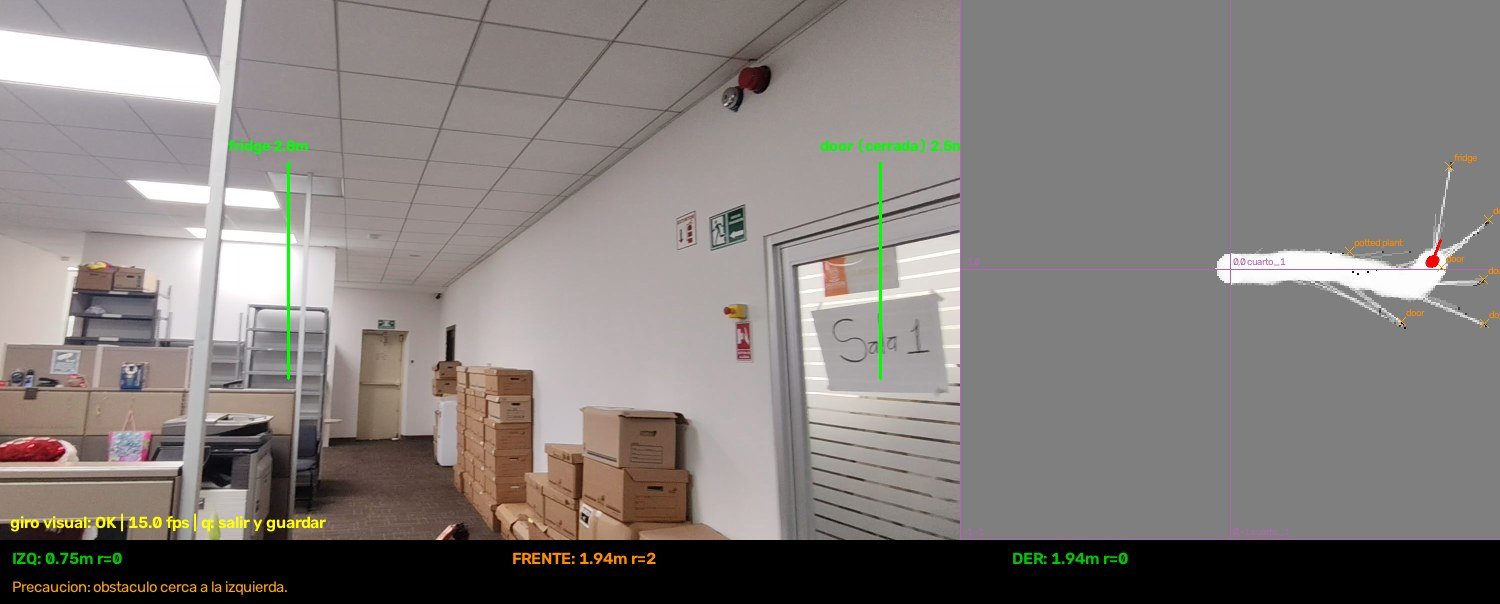
\includegraphics[width=\textwidth]{Capturas_TT2/cap_oficina_f241.jpg}
    \caption{Inicio del recorrido. Se detectan una puerta cerrada a 2.5~m y un
    refrigerador, el mapa empieza a registrar la franja recorrida y la barra avisa de un
    obstáculo a 0.75~m a la izquierda.}
    \label{fig:cap_oficina_1}
\end{figure}

\begin{figure}[H]
    \centering
    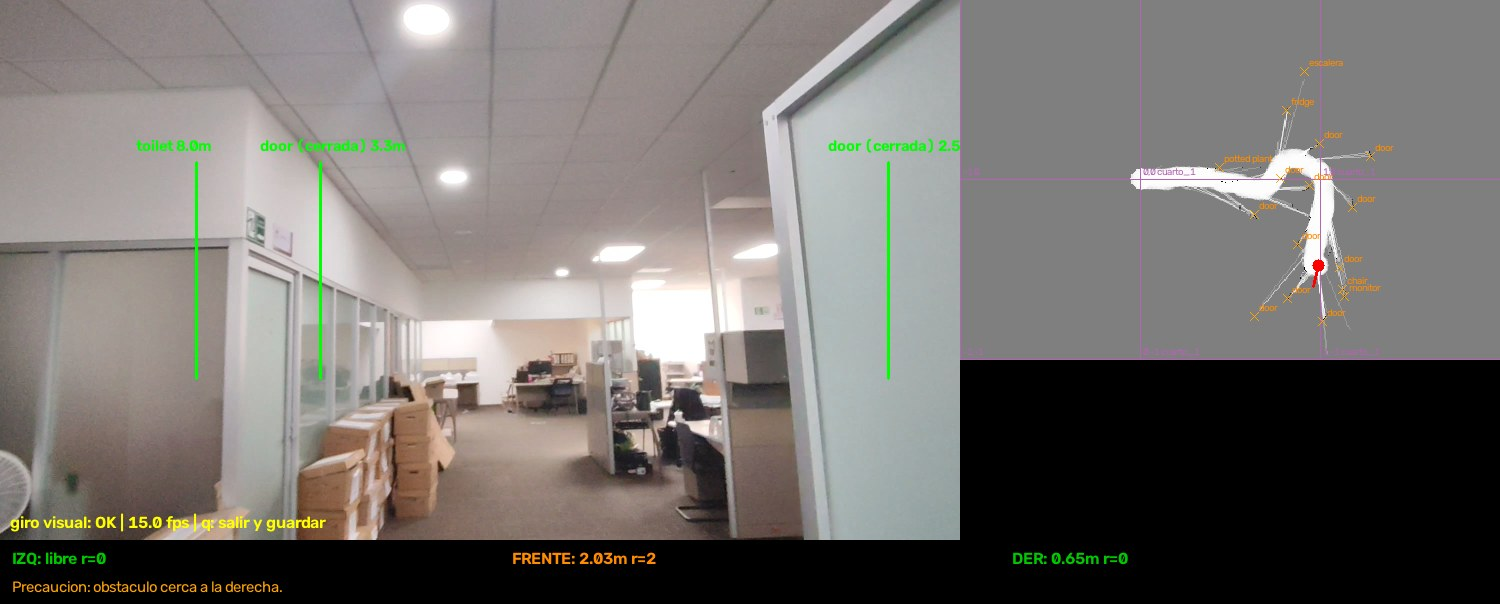
\includegraphics[width=\textwidth]{Capturas_TT2/cap_oficina_f481.jpg}
    \caption{Al girar hacia el pasillo, el SLAM ya mantiene varias puertas como
    \emph{landmarks} y el mapa muestra el cambio de dirección.}
    \label{fig:cap_oficina_2}
\end{figure}

\begin{figure}[H]
    \centering
    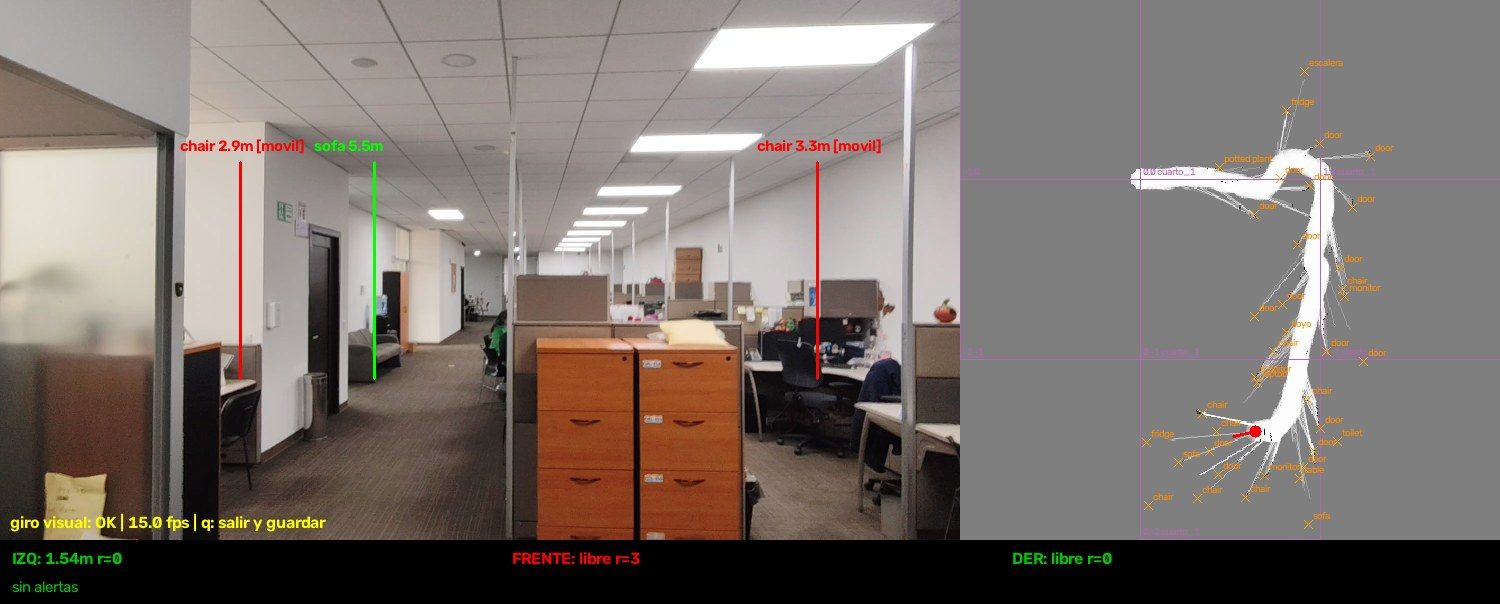
\includegraphics[width=\textwidth]{Capturas_TT2/cap_oficina_f901.jpg}
    \caption{Final del recorrido, con siete bloques y 39 \emph{landmarks} confirmados.
    Dos sillas aparecen como móviles por un error del rastreador al avanzar el
    usuario.}
    \label{fig:cap_oficina_3}
\end{figure}

En las capturas se ven también errores de la percepción que llegan a la
representación. En la Figura~\ref{fig:cap_oficina_2} aparece un inodoro a 8~m que no
existe, y en la Figura~\ref{fig:cap_oficina_3} dos sillas que no se mueven se marcan como
móviles, porque el rastreador compensa el giro del usuario pero no su avance. Las reglas
del SLAM contienen el daño, ya que los objetos móviles no se usan como \emph{landmarks}
y los falsos positivos aislados no llegan a los avistamientos necesarios para
confirmarse.

\subsection{Funcionamiento en el prototipo}

\TODO{capturas o registros de \texttt{main\_pi.py} durante un recorrido con el
prototipo: mapa resultante, \emph{landmarks}, alertas emitidas y comentarios del
recorrido}.

\subsection{Tiempos de procesamiento}

La Tabla~\ref{tab:tiempos_ciclo} desglosa el tiempo promedio por ciclo. La columna de
la computadora portátil se midió al procesar el video de la oficina (456 cuadros, uno de
cada dos del video original) con todos los modelos en CPU; la de la Raspberry Pi
corresponde al prototipo en operación.

\begin{table}[H]
\centering
\caption{Tiempo promedio por ciclo}
\label{tab:tiempos_ciclo}
\renewcommand{\arraystretch}{1.2}
\begin{tabular}{|p{7.4cm}|c|c|}
\hline
\textbf{Etapa} & \textbf{Apple M4 (ms)} & \textbf{Raspberry Pi (ms)} \\
\hline
Estimación de giro y caminata por flujo óptico & 5.4 & \TODO{} \\
Detección de objetos (YOLOv8s-seg) & 92.4 & \TODO{} \\
Segmentación de peligros y puertas (SegFormer, amortizado) & 77.5 & \TODO{} \\
\hline
SLAM (EKF, asociación y gestión de \emph{landmarks}) & 0.27 & \TODO{} \\
Ray Casting y actualización del mapa por bloques & 0.23 & \TODO{} \\
Construcción del cuadro de navegación & 0.51 & \TODO{} \\
\hline
\textbf{Subtotal de los módulos de representación} & \textbf{1.01} & \TODO{} \\
\hline
\end{tabular}
\end{table}

Los módulos de representación se llevan alrededor de un milisegundo por ciclo en la
computadora portátil, menos del 1\,\% del tiempo total. Por sí solos podrían correr a
cientos de hertz, muy por encima de los 10~Hz que pide RNF-03; el cuello de botella es la
percepción visual. Por eso el SLAM y el mapa siguen actualizándose con la odometría en
los ciclos en que la visión no entrega resultados, y la segmentación solo se ejecuta cada
cierto número de cuadros. En la Raspberry Pi el ciclo completo corre a \TODO{frecuencia
del ciclo completo en la Raspberry Pi}.

\subsection{Cumplimiento de requerimientos}

La Tabla~\ref{tab:req_representacion} relaciona los requerimientos de los módulos de
representación con su estado.

\begin{longtable}{|p{1.6cm}|p{4.2cm}|p{2.4cm}|p{6.2cm}|}
\caption{Estado de los requerimientos de los módulos de representación}
\label{tab:req_representacion} \\
\hline
\textbf{Req.} & \textbf{Descripción breve} & \textbf{Estado} & \textbf{Evidencia} \\
\hline
\endfirsthead
\hline
\textbf{Req.} & \textbf{Descripción breve} & \textbf{Estado} & \textbf{Evidencia} \\
\hline
\endhead
RF-14 & Estimación continua de la pose & Cumplido & EKF con ATE de 0.21~m en
simulación y error acotado con odometría sesgada (Tabla~\ref{tab:slam_deriva}). \\
\hline
RF-15 & Mapa incremental sin mapa previo & Cumplido &
Figura~\ref{fig:mapeo_evolucion} y mapas de 19 videos reales. \\
\hline
RF-16 & Zonas libres y ocupadas & Cumplido & Mapa log-odds con tres estados, capa de
peligros y mapa local de dos canales. \\
\hline
RF-17 & Actualización dinámica & Cumplido & Los obstáculos nuevos aparecen en el mapa;
los que desaparecen se liberan con ecos precisos y los falsos peligros de piso, con los
rayos de piso libre (Secciones~\ref{sec:dev_ray} y \ref{sec:dev_mapeo}). \\
\hline
RNF-03 & Mapa a 10~Hz o más & \TODO{} & 1~ms por ciclo en la computadora portátil
(Tabla~\ref{tab:tiempos_ciclo}); \TODO{frecuencia en la Raspberry Pi}. \\
\hline
RNF-05 & Hardware limitado & \TODO{} & Estado de pose de tamaño fijo y memoria acotada a
25 bloques (unos 3~MB); \TODO{uso de memoria y CPU en la Raspberry Pi}. \\
\hline
RNF-09 & Comportamiento conservador & Cumplido & Confianza que baja sin correcciones
(Figura~\ref{fig:slam_incertidumbre}) y distancia mínima por sector. \\
\hline
RNF-13 & Operación sin internet & Cumplido & Ningún módulo de representación necesita
conexión y los mapas se guardan localmente. \\
\hline
RNF-14 & Modularidad & Cumplido & Comunicación solo por las estructuras de
\texttt{interfaces.py}; el mismo código trabaja con cámara, video y simulación. \\
\hline
\end{longtable}


% ==============================================================================
\section{Módulo de navegación}
\label{sec:dev_nav}
% ==============================================================================

\subsection{Descripción}

El módulo de navegación decide, paso a paso, qué debe hacer el usuario para llegar a
su destino: avanzar, girar a la izquierda, girar a la derecha o detenerse. La decisión
la toma un agente de aprendizaje por refuerzo profundo entrenado en simulación con el
algoritmo PPO, tal como se planteó en TT1. Alrededor del agente se construyeron tres
piezas que no estaban en el diseño original: un ejecutor que administra la sesión y
traduce las acciones en frases, una capa de seguridad determinística que puede
anular al agente y un planificador que anticipa la ruta completa para mostrarla en la
interfaz. El módulo cubre los requerimientos RF-18 a RF-21 y RF-23.

Los destinos ya no provienen de un servicio de cartografía. Cuando el usuario pide
``llévame a la salida'', el ejecutor busca entre los \emph{landmarks} del SLAM el más
cercano con la etiqueta correspondiente (puerta, en este caso) y lo toma como meta.
También se acepta un punto explícito del mapa, lo cual se usa durante las pruebas.

\subsection{Entorno de entrenamiento}

El agente se entrena en un entorno propio construido con Gymnasium
(\texttt{navigation/nav\_env.py}). Cada episodio genera un mundo nuevo de uno de tres
tipos:

\begin{itemize}
    \item \textbf{Cuarto} (40\,\% de los episodios): un rectángulo de 4 a 9~m por 3.5 a
    7~m con entre dos y cinco muebles, hasta un peligro de piso y hasta una persona en
    movimiento.
    \item \textbf{Dos cuartos con puerta} (35\,\%): dos cuartos separados por una pared
    con un vano de 0.9 a 1.3~m. El inicio está en un cuarto y la meta en el otro, de
    modo que el agente debe encontrar la puerta.
    \item \textbf{Exterior} (25\,\%): un área abierta de 10 a 18~m por 8 a 14~m con
    postes dispersos, de una a tres coladeras y hasta dos personas.
\end{itemize}

Las personas se desplazan entre 5 y 12~cm por paso, rebotan en los límites y de vez
en cuando cambian de dirección. Los peligros de piso no bloquean los rayos, igual que
en el sistema real, donde un hoyo no produce eco ni detiene la vista: el agente solo
los conoce por la distancia por sector que le llega en la observación. Además de los
mundos generados, en aproximadamente la mitad de los episodios se usa uno de los 19
mapas reales obtenidos de video (Sección~\ref{sec:dev_mapeo}). Para ello, las celdas
ocupadas se convierten en obstáculos circulares, la capa de peligros en coladeras, y
el inicio y la meta se eligen dentro de la misma zona libre conexa, con al menos
30~cm de holgura respecto a cualquier obstáculo.

\subsection{Acciones, observación y recompensa}

Las acciones son las cuatro definidas en TT1: avanzar 0.30~m, girar $20^\circ$ a la
izquierda, girar $20^\circ$ a la derecha y detenerse.

La observación es donde más se apartó la implementación del diseño original. El
vector de ocho valores planteado en TT1 ($d_{\text{front}}$, $d_{\text{left}}$,
$d_{\text{right}}$, $\phi_{\text{goal}}$, $d_{\text{goal}}$ y los tres riesgos) se
implementó y se comparó contra una observación extendida de 24 valores, descrita en la
Tabla~\ref{tab:nav_obs}. Con el mismo presupuesto de entrenamiento, la observación
extendida obtuvo 85.8\,\% de episodios exitosos contra 44.2\,\% de la original
(Figura~\ref{fig:nav_comparacion}). La diferencia se concentra en los mundos con
puerta: con solo tres distancias por sector, el agente no ``ve'' el hueco de la puerta
y fracasa en nueve de cada diez intentos.

\begin{table}[H]
\centering
\caption{Componentes de la observación extendida (24 valores normalizados)}
\label{tab:nav_obs}
\renewcommand{\arraystretch}{1.25}
\begin{tabular}{|c|p{11.8cm}|}
\hline
\textbf{Valores} & \textbf{Contenido} \\
\hline
11 & Distancia libre en 11 direcciones entre $-100^\circ$ y $+100^\circ$, divididas
entre el alcance máximo de 4~m. \\
\hline
3 & Distancia al peligro de piso más cercano en cada sector (frente, izquierda,
derecha), divididas entre 3~m. \\
\hline
3 & Nivel de riesgo por sector, dividido entre 3. \\
\hline
3 & Dirección a la meta como $\sin\phi_{\text{goal}}$ y $\cos\phi_{\text{goal}}$, y
distancia a la meta acotada a 10~m. \\
\hline
4 & Acción anterior en codificación \emph{one-hot}. \\
\hline
\end{tabular}
\end{table}

\begin{figure}[H]
    \centering
    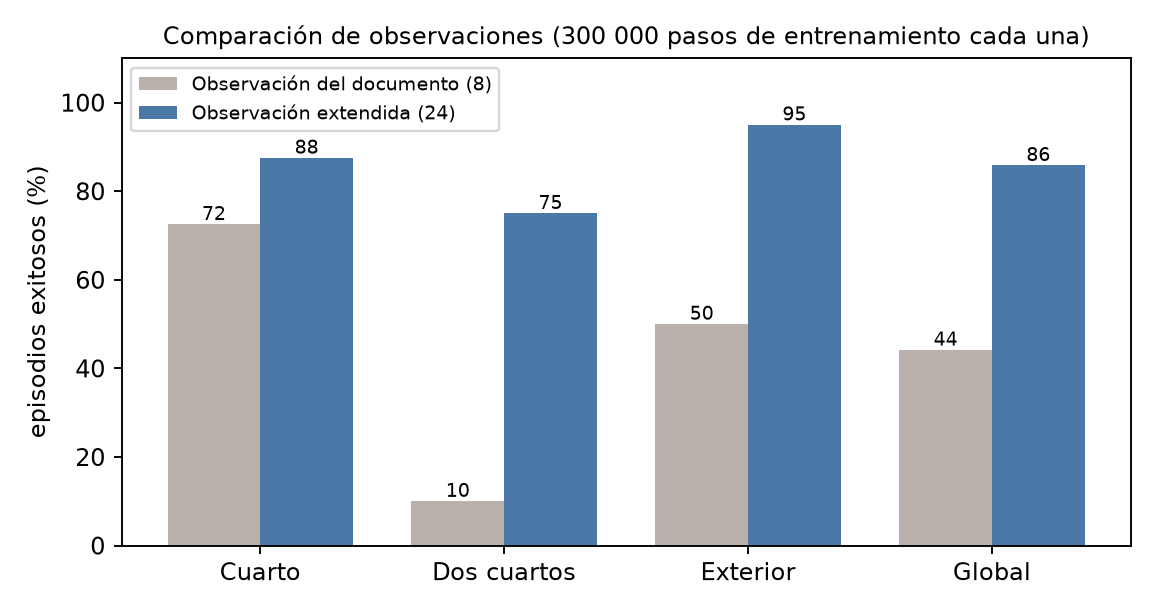
\includegraphics[width=0.78\textwidth]{Capturas_TT2/nav/nav_comparacion_obs.png}
    \caption{Porcentaje de episodios exitosos con la observación del documento y con la
    observación extendida, tras 300\,000 pasos de entrenamiento cada una.}
    \label{fig:nav_comparacion}
\end{figure}

La recompensa sigue la estructura de TT1, pero con escalas ajustadas. Con los
coeficientes originales, la penalización por riesgo pesaba tanto que el agente
aprendía a quedarse quieto. La versión final es:

\[
r_t = -0.1 + 4\,(d_{t-1} - d_t) - 0.15\, r_{\text{front}}
      + \begin{cases}
      +100 & \text{si llega a menos de 0.45~m de la meta} \\
      -100 & \text{si choca o cae en un peligro de piso} \\
      +0.5 & \text{si se detiene con una persona a menos de 1.2~m enfrente} \\
      -0.3 & \text{si se detiene sin motivo}
      \end{cases}
\]

donde $d_t$ es la distancia a la meta. El término de detenerse se agregó para que la
acción tuviera una función clara: esperar a que una persona termine de cruzar.

Para reducir la diferencia entre la simulación y el sistema real se añadió ruido de
5\,\% a las distancias, de $2^\circ$ al ángulo de la meta y, en el 8\,\% de los rayos
bloqueados, se reporta el alcance máximo como si estuvieran libres. Esta última
perturbación imita lo que ocurre en el mapa real, donde un rayo delgado puede colarse
entre dos celdas de eco separadas (Sección~\ref{sec:dev_ray}) y reportar libre un
frente bloqueado.

\subsection{Entrenamiento}

El agente se entrena con la implementación de PPO de Stable-Baselines3 sobre
PyTorch, con ocho entornos en paralelo. La Tabla~\ref{tab:nav_ppo} resume los
hiperparámetros. El modelo final se entrenó durante 8 millones de pasos. Se exporta en
dos formatos: el archivo completo de Stable-Baselines3, que se usa en la computadora
portátil, y un archivo con solo los pesos de la red del actor, con el que la
Raspberry Pi ejecuta la inferencia en NumPy sin instalar PyTorch. Se verificó que
ambos formatos eligen la misma acción en 500 observaciones aleatorias.

\begin{table}[H]
\centering
\caption{Hiperparámetros de PPO}
\label{tab:nav_ppo}
\renewcommand{\arraystretch}{1.2}
\begin{tabular}{|l|c|}
\hline
\textbf{Parámetro} & \textbf{Valor} \\
\hline
Red del actor y del crítico & dos capas ocultas de 128 neuronas, \emph{tanh} \\
Pasos por actualización (por entorno) & 2048 \\
Tamaño de lote & 512 \\
Factor de descuento $\gamma$ & 0.995 \\
$\lambda$ de GAE & 0.95 \\
Coeficiente de entropía & 0.01 \\
Tasa de aprendizaje & $3 \times 10^{-4}$ \\
Recorte de PPO & 0.2 \\
\hline
\end{tabular}
\end{table}

El modelo pasó por varias iteraciones, evaluadas siempre con el mismo protocolo. Un
primer modelo entrenado solo en mundos generados alcanzó 99.2\,\% de éxito en ellos.
Al incorporar los mapas de video, el peor caso fue un pasillo de oficina muy angosto y
lleno de muebles (v09), donde varios reentrenamientos con más pasos o con otra mezcla
de mapas no lograron superar al modelo vigente. Al revisar ese caso se encontró un
error en el entrenador: en mapas densos el inicio o la meta podían quedar encima de un
obstáculo, lo que producía choques imposibles de evitar. Con el muestreo corregido, el
modelo vigente subió de 82.5 a 85\,\% en ese mapa, y se comprobó que retirar v09 del
entrenamiento empeora el desempeño en pasillos densos, por lo que se conservó en la
mezcla.

\subsection{Ejecución en el dispositivo}

El ejecutor (\texttt{navigation/navigator.py}) es la parte del módulo que corre en el
dispositivo. Mantiene el estado de la sesión (en espera, activa o pausada) con los
mensajes literales del Algoritmo 11 de TT1, recibe los comandos ya interpretados por
el PLN y, en cada ciclo, construye la observación a partir del cuadro de navegación y
del mapa. Para que esa observación se parezca a la del entrenamiento, cada uno de los
11 rayos es el mínimo de un abanico de tres sub-rayos separados $6^\circ$, y las
distancias a los peligros se leen del segundo canal del mapa local.

Sobre la decisión del agente actúan varias reglas fijas:

\begin{itemize}
    \item \textbf{Capa de seguridad.} Si el agente indica avanzar y la distancia libre
    al frente es menor que 0.80~m, ya sea según el mapa o según la visión, la orden se
    reemplaza por un giro. El umbral es el mismo de la alerta crítica, de modo que el
    usuario nunca escucha ``Deténgase'' y ``Avance'' en el mismo instante. El sentido
    del giro se mantiene durante un máximo de ocho giros seguidos (unos $160^\circ$),
    para no alternar izquierda y derecha en una esquina.
    \item \textbf{Ritmo de decisión.} El agente decide una vez por segundo, salvo que
    haya una alerta crítica, en cuyo caso decide de inmediato.
    \item \textbf{Frases.} Cada acción se traduce con las frases exactas de TT1:
    ``Avance N metros'', ``Gire ligeramente a la izquierda'' (giros de hasta
    $45^\circ$), ``Gire a la izquierda N grados'' o ``Deténgase''. La distancia de
    avance se limita a lo que el mapa ve libre y, si la confianza del SLAM baja de
    0.35, a un metro. El aviso ``Está cerca de su destino'' se dice una sola vez por
    destino.
    \item \textbf{Llegada.} La sesión termina cuando la pose queda a menos de 0.6~m de
    la meta o cuando la cámara ve el objeto buscado a menos de 1~m enfrente. La
    segunda condición se agregó porque, sin odometría, la pose deriva y el usuario
    podía quedarse dando vueltas junto al objeto.
    \item \textbf{Bloqueo.} Si en 20~s la distancia a la meta no disminuye al menos
    30~cm, el sistema avisa que no encuentra un paso libre y sugiere pedir otra ruta.
\end{itemize}

El Algoritmo~\ref{alg:dev_nav} resume un ciclo del ejecutor.

\begin{center}
\captionof{algorithm}{Ciclo del ejecutor de navegación}
\label{alg:dev_nav}
\end{center}
\vspace{-1.8cm}
\rule{\textwidth}{0.4pt}
\vspace{-0.9cm}
\begin{algorithmic}[1]

\Statex \textbf{ENTRADA:} cuadro\_nav, mapa, alertas
\Statex \textbf{SALIDA:} lista de mensajes para la salida de voz

\Statex
\If{sesión no está activa}
    \State \Return []
\EndIf
\State d $\gets$ distancia(pose, meta)
\If{d $< 0.6$ m O la cámara ve el objeto meta a menos de 1 m}
    \State sesión $\gets$ ``en\_espera''
    \State \Return [``Ha llegado a su destino.'']
\EndIf
\If{no hay alerta crítica Y pasó menos de 1 s desde la última decisión}
    \State \Return []
\EndIf
\State obs $\gets$ construir\_observación(cuadro\_nav, mapa, meta, acción\_previa)
\State acción $\gets$ política(obs)
\If{acción = avanzar Y distancia\_libre\_al\_frente $< 0.80$ m}
    \State acción $\gets$ giro\_forzado() \Comment{con histéresis de sentido}
\EndIf
\State texto $\gets$ frase(acción, d, $\phi_{\text{goal}}$, distancia\_libre, confianza)
\If{texto es nuevo O pasaron más de 3.5 s desde la última indicación}
    \State agregar texto a mensajes
\EndIf
\If{la distancia a la meta no bajó 0.3 m en 20 s}
    \State agregar aviso de bloqueo a mensajes
\EndIf
\State \Return mensajes

\end{algorithmic}
\vspace{-0.9cm}
\rule{\textwidth}{0.4pt}

\subsection{Planificador de ruta}

El agente decide solo el siguiente paso, lo cual dificulta saber hacia dónde va.
Para visualizarlo, el planificador (\texttt{navigation/route\_planner.py}) simula al
agente sobre el mapa actual desde la pose del usuario, sin moverlo, y registra los
puntos por los que pasaría hasta llegar, quedar atascado o agotar 240 pasos. La ruta
resultante se clasifica como ``llega'', ``bloqueada'' o ``larga'' y se dibuja en la
interfaz. Un plan tarda unos 7~ms; se recalcula cada dos segundos en un hilo aparte, o
de inmediato si llega una alerta crítica. Como las puertas se registran sobre la
pared, cuando la meta cae en una celda ocupada el planificador la traslada a la celda
libre más cercana. La ruta es informativa: la decisión que se le comunica al usuario
sigue siendo la del ejecutor.

\subsection{Resultados}

\textbf{Evaluación del modelo.} El modelo final se evaluó en 880 episodios: 40 en
cada tipo de mundo generado y 40 en cada uno de los 19 mapas reales, con semillas
distintas a las del entrenamiento. Llegó a la meta en el 97.8\,\% de los episodios,
chocó en el 2.0\,\%, nunca cayó en un peligro de piso y solo un episodio agotó el
límite de pasos. Los episodios exitosos tomaron en promedio 27 pasos. La
Figura~\ref{fig:nav_eval} muestra el desglose por mundo; el único mapa por debajo del
90\,\% es el pasillo denso v09 (85\,\%).

\begin{figure}[H]
    \centering
    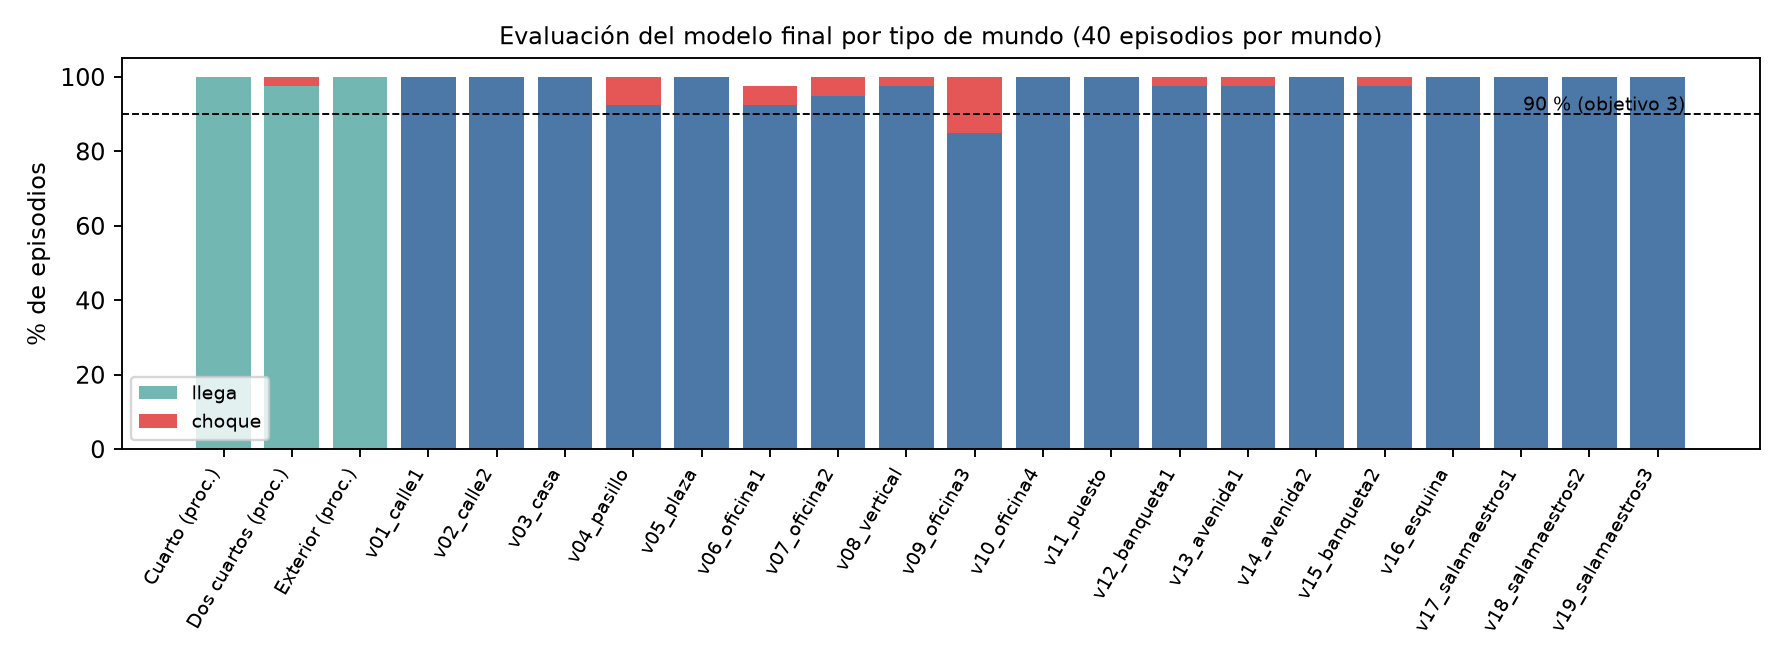
\includegraphics[width=\textwidth]{Capturas_TT2/nav/nav_eval_mundos.png}
    \caption{Porcentaje de episodios exitosos y con choque por mundo. En verde claro,
    mundos generados; en azul, mapas obtenidos de videos reales.}
    \label{fig:nav_eval}
\end{figure}

La Figura~\ref{fig:nav_episodios} muestra un episodio de cada tipo de mundo generado.
En el de dos cuartos, el agente se dirige primero hacia la puerta y cruza el vano; en
el exterior se aleja de las coladeras, aunque estas no aparecen en sus rayos.

\begin{figure}[H]
    \centering
    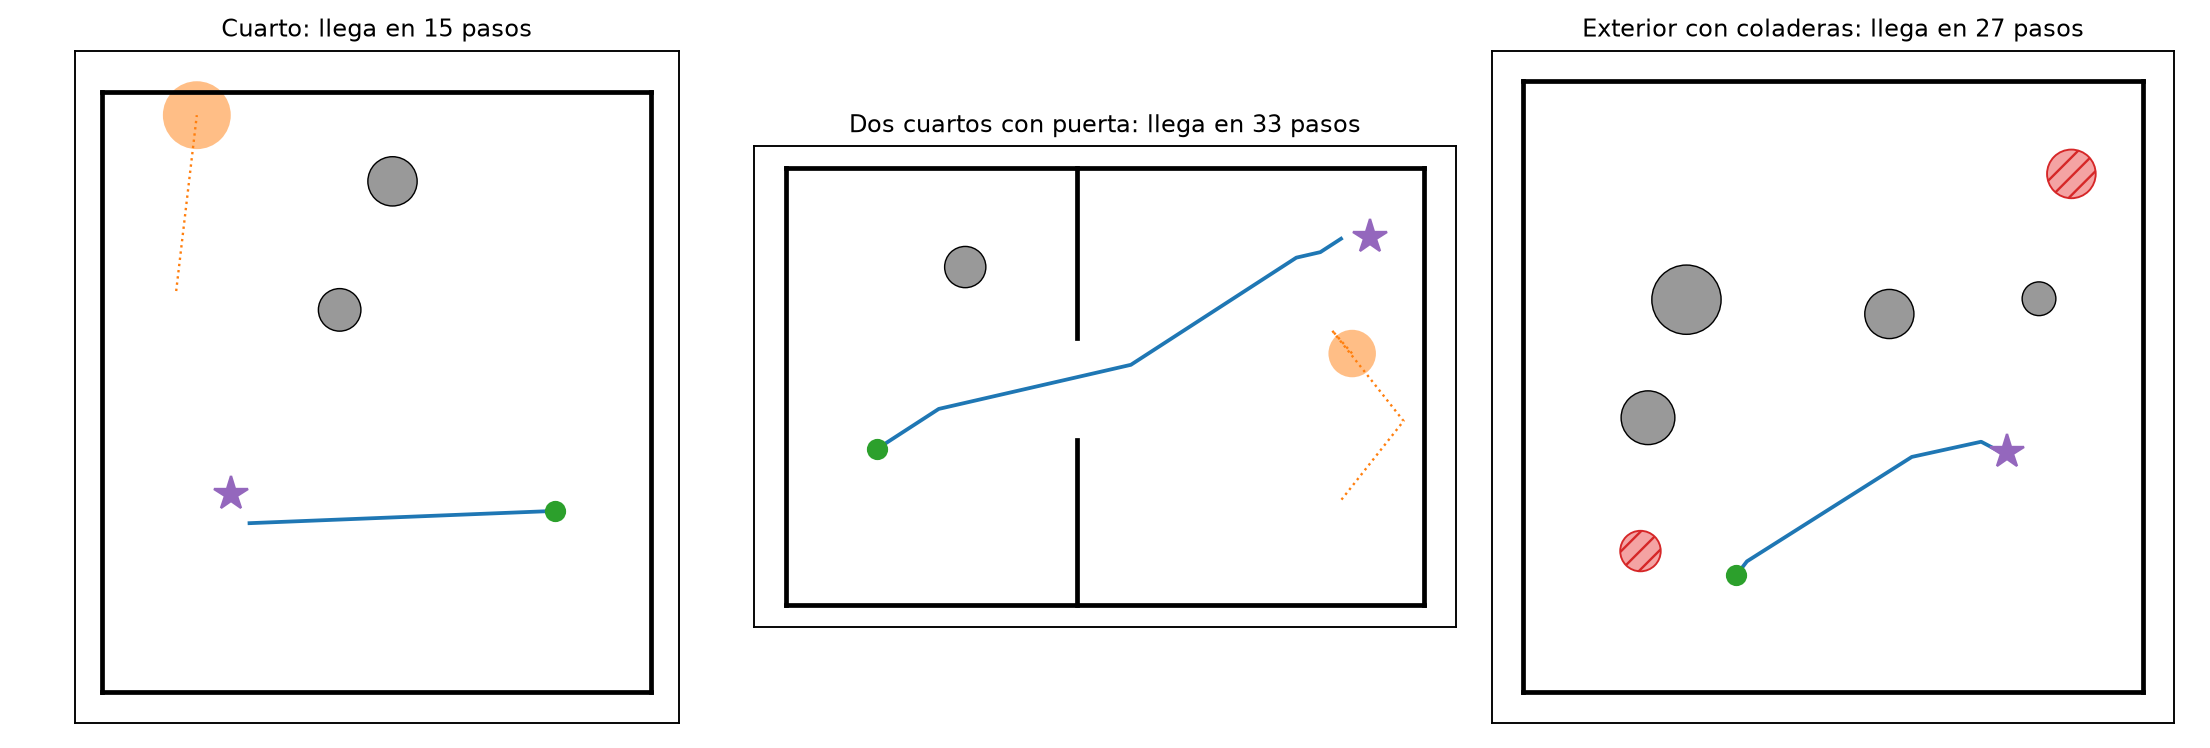
\includegraphics[width=\textwidth]{Capturas_TT2/nav/nav_episodios.png}
    \caption{Episodios del modelo final. Punto verde: inicio; estrella: meta; gris:
    obstáculos; rojo rayado: peligros de piso; naranja: persona en movimiento y su
    recorrido.}
    \label{fig:nav_episodios}
\end{figure}

\textbf{Sesiones completas en lazo cerrado.} La evaluación anterior mide al agente
dentro de su propio simulador. Para probar la cadena completa se ejecutaron sesiones
en el cuarto simulado con todos los módulos reales: sensores simulados, SLAM, mapa,
PLN, ejecutor y salida amigable. Un usuario virtual primero recorre el cuarto para
construir el mapa, después pide un destino por texto y a partir de ahí hace
exactamente lo que le indica el sistema. Se realizaron 20 sesiones (cinco semillas por
cuatro destinos) y en cada una se midió la distancia real entre el usuario y la
superficie del objeto en el momento en que el sistema anunció la llegada.

El sistema anunció la llegada en las 20 sesiones y el usuario nunca chocó, pero solo
en 7 quedó a menos de 1~m del objeto y en 12 a menos de 1.5~m. Al registrar qué
condición disparó cada llegada se encontró la causa (Tabla~\ref{tab:nav_lazo}): en 17
sesiones la llegada la decidió la regla de percepción, porque en un solo cuadro la
estimación monocular ubicó al objeto a menos de 1~m cuando en realidad estaba hasta a
2.5~m. Las tres llegadas decididas por la distancia en el mapa terminaron a menos de
0.8~m del objeto.

También se revisó si la validación con los ultrasónicos intervino en esas llegadas.
En 16 de las 17 el objeto quedaba fuera del cono angosto de los sensores (unos
$\pm 20^\circ$, mientras que la regla acepta objetos hasta $\pm 60^\circ$) o por
debajo del haz, así que el ultrasonido no pudo confirmar ni contradecir la distancia.
La única llegada con el objeto confirmado por ambos sensores terminó a 0.99~m, que es
una llegada correcta.

\begin{table}[H]
\centering
\caption{Sesiones en lazo cerrado según la condición que disparó la llegada}
\label{tab:nav_lazo}
\renewcommand{\arraystretch}{1.2}
\begin{tabular}{|p{5.2cm}|c|c|c|}
\hline
\textbf{Condición de llegada} & \textbf{Sesiones} & \textbf{Distancia real promedio}
& \textbf{A menos de 1~m} \\
\hline
Pose a menos de 0.6~m de la meta & 3 & 0.55~m & 3 \\
Objeto visto a menos de 1~m & 17 & 1.56~m & 4 \\
\hline
\textbf{Total} & \textbf{20} & & \textbf{7} \\
\hline
\end{tabular}
\end{table}

La regla de percepción resolvió un problema real, pero tal como está implementada es
demasiado sensible: basta un cuadro con un error monocular de 25 a 50\,\% para terminar
la sesión antes de tiempo. Exigir la condición durante varios cuadros seguidos, pedir
que el ultrasonido la confirme cuando el objeto está dentro de su cono, o combinarla
con la distancia en el mapa debería corregirlo.

La Figura~\ref{fig:nav_sesion} muestra una de estas sesiones. El usuario pidió
``llévame al sillón'' y en el paso 45 apareció una caja a 1.2~m delante de él. El
planificador cambió la ruta para pasar por debajo de la caja y el usuario siguió las
indicaciones hasta quedar a 0.75~m del sillón, donde la regla de percepción dio por
terminada la sesión. En corridas anteriores de la misma prueba se observó que el
primer plan después de la caja a veces todavía la atravesaba: el mapa necesita varios
ecos para convertir en ocupada una celda que ya había visto libre muchas veces
(Figura~\ref{fig:ray_logodds}).

\begin{figure}[H]
    \centering
    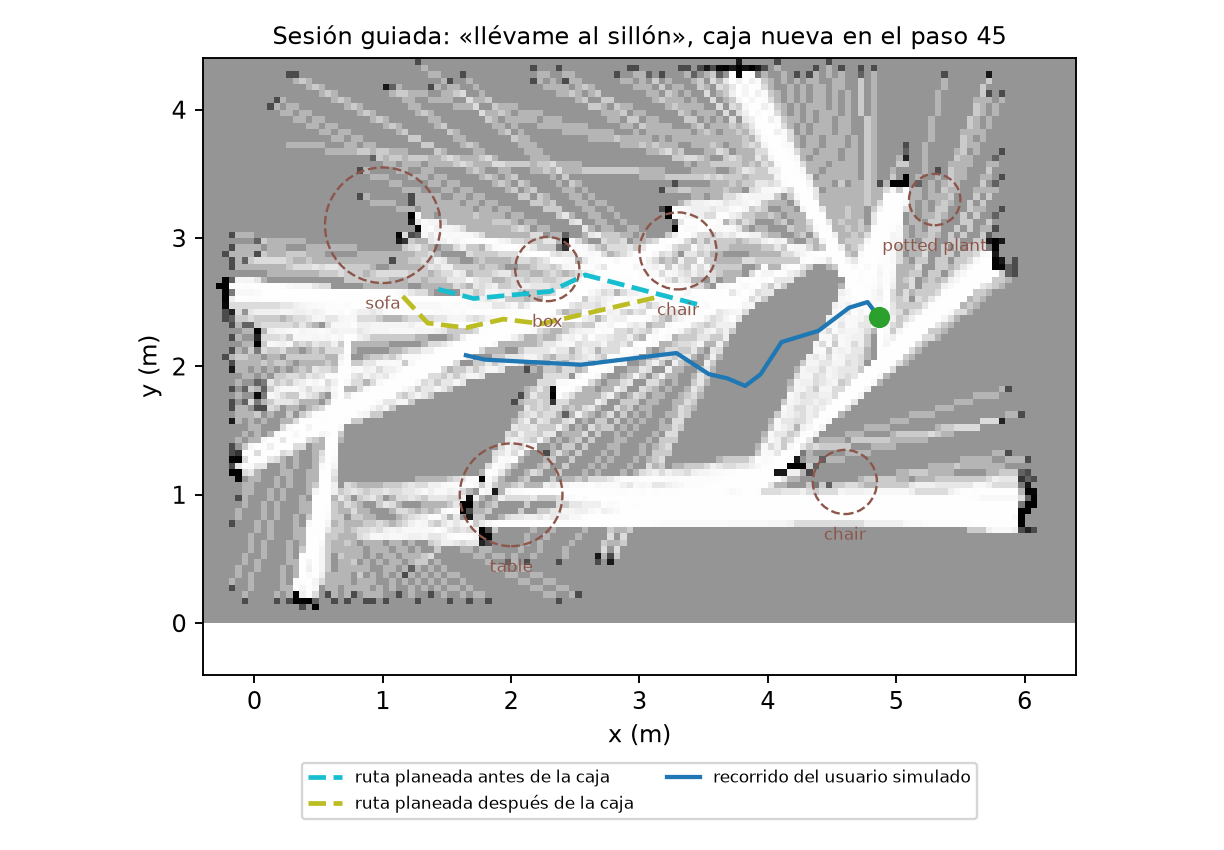
\includegraphics[width=0.82\textwidth]{Capturas_TT2/nav/nav_sesion_ok.png}
    \caption{Sesión en lazo cerrado con una caja que aparece en el camino. Las líneas
    discontinuas son las rutas que calculó el planificador antes y después de la
    caja.}
    \label{fig:nav_sesion}
\end{figure}

La Figura~\ref{fig:nav_vivo} muestra la vista de ruta de la interfaz de
\texttt{main\_nav\_lap.py} en dos momentos de esa sesión. En la segunda captura se
aprecia otro efecto del SLAM: el mapa ligero contiene \emph{landmarks} duplicados
(dos mesas y dos sillones en un cuarto que tiene uno de cada uno).

\begin{figure}[H]
    \centering
    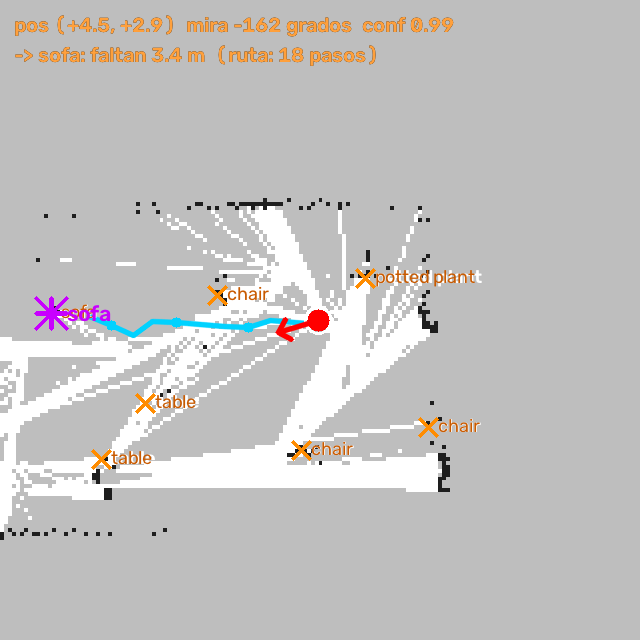
\includegraphics[width=0.48\textwidth]{Capturas_TT2/nav/nav_vivo_p10.png}
    \hfill
    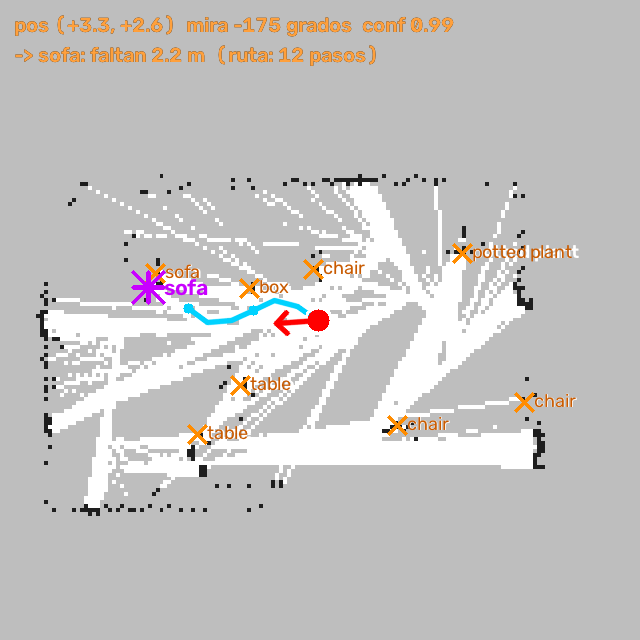
\includegraphics[width=0.48\textwidth]{Capturas_TT2/nav/nav_vivo_p52.png}
    \caption{Vista de ruta en vivo al inicio de la sesión (izquierda) y después de la
    caja (derecha). Cian: ruta planeada; estrella magenta: meta; cruces naranjas:
    \emph{landmarks}.}
    \label{fig:nav_vivo}
\end{figure}

Durante las sesiones se observaron otros dos detalles. Como en la simulación el
agente decide en cada ciclo, el sistema emitió en promedio una indicación cada 1.8
pasos, lo que en uso real sería demasiado; en el dispositivo el ritmo es de una
decisión por segundo y las indicaciones repetidas se agrupan. Además, el mensaje
amigable de llegada dice ``¡Llegamos! Ya estás en sofa'', porque usa la etiqueta en
inglés del \emph{landmark} en lugar del nombre que dijo el usuario.

\textbf{Costo computacional.} Construir la observación toma 0.64~ms, la inferencia
de la política 0.06~ms con Stable-Baselines3 y 0.01~ms con NumPy, y un plan completo
de ruta 7~ms. La navegación no limita la frecuencia del sistema.

\subsection{Limitaciones}

\begin{itemize}
    \item La llegada por percepción se dispara con un solo cuadro y termina sesiones
    antes de tiempo.
    \item Los resultados del 97.8\,\% corresponden al simulador del agente. En lazo
    cerrado con el SLAM y la percepción simulados, la llegada correcta a menos de 1~m
    bajó a 7 de 20 sesiones. Aún no se ha probado con una persona real.
    \item El riesgo por sector se calcula distinto en entrenamiento (a partir de la
    distancia a cualquier obstáculo) y en el sistema real (a partir de las
    detecciones de visión). Se intentó alinear el sistema real con la regla del
    entrenamiento y el desempeño empeoró, por lo que la corrección pendiente es del
    lado del entrenamiento.
    \item La solicitud de ruta alternativa reinicia el seguimiento del progreso, pero no
    obliga al agente a tomar un camino distinto.
    \item Los modelos de ruido del simulador se ajustaron sin los sensores físicos; al
    montar la IMU y los MB1232 habrá que medir el ruido real y reentrenar.
\end{itemize}


% ==============================================================================
\section{Módulo de alertas}
\label{sec:dev_alertas}
% ==============================================================================

\subsection{Descripción}

El módulo de alertas es la capa de seguridad del sistema y corresponde al Algoritmo 7
de TT1. La navegación solo trabaja cuando hay una ruta activa, pero las alertas están
encendidas todo el tiempo, así que una persona puede usar los lentes sin pedir ningún
destino y aun así enterarse de lo que tiene enfrente. El módulo atiende RF-12, RF-20,
RNF-01, RNF-09 y RNF-12.

En cada ciclo, \texttt{alertas.py} lee el cuadro de navegación y regresa la lista de
alertas nuevas, cada una con su prioridad, junto con una bandera que indica si hay que
recalcular la ruta. También se encarga del sonido. Para esa parte se integró el módulo
de pitidos que desarrolló el equipo (\texttt{VozYPLN/alertas.py}), y gracias a él las
alertas no se confunden con las indicaciones de navegación. Una precaución es solo un
pitido estéreo, mientras que una alerta crítica es un pitido seguido de una frase corta
que interrumpe cualquier otra cosa que el sistema esté diciendo.

\subsection{Reglas de alerta}

La Tabla~\ref{tab:alertas_reglas} reúne las reglas. Los umbrales del frente (0.80~m
para la alerta crítica y 1.50~m para la precaución) son los definidos en TT1. En los
costados los umbrales son menores, porque caminar a 60~cm de una pared es lo más normal
en un pasillo y no amerita una alerta crítica. La excepción son las detecciones de
riesgo alto, que usan los umbrales del frente en cualquier sector.

\begin{longtable}{|p{3.4cm}|p{3.6cm}|p{3.2cm}|p{4.3cm}|}
\caption{Reglas del módulo de alertas}
\label{tab:alertas_reglas} \\
\hline
\textbf{Situación} & \textbf{Crítica} & \textbf{Precaución} & \textbf{Ejemplo de
frase} \\
\hline
\endfirsthead
\hline
\textbf{Situación} & \textbf{Crítica} & \textbf{Precaución} & \textbf{Ejemplo de
frase} \\
\hline
\endhead
Obstáculo al frente (mapa o visión) & $< 0.80$~m & $< 1.50$~m & ``Atención:
obstáculo a 80 centímetros al frente. Deténgase.'' \\
\hline
Obstáculo a un costado & $< 0.45$~m & $< 0.80$~m & ``Precaución: obstáculo cerca a
la izquierda.'' \\
\hline
Persona u objeto en movimiento (hasta 2~m) & $< 1.0$~m & de 1.0 a 2.0~m & ``Alto. Se
acerca una persona al frente, muy cerca.'' \\
\hline
Hoyo, agua o escalera al frente (hasta 2.5~m) & $< 1.3$~m & de 1.3 a 2.5~m &
``Atención: un hoyo adelante, a unos 2 pasos.'' \\
\hline
Eco ultrasónico que ninguna detección confirmada explica & $< 0.80$~m & de 0.80 a
1.50~m & ``Atención: pared al frente a 60 centímetros. Deténgase.'' \\
\hline
Detección contradicha por el ultrasonido (al frente) & --- & $< 1.5$~m & ``Posible
silla al frente (solo cámara).'' \\
\hline
Lectura directa de un sensor de proximidad & $< 1.0$~m & de 1.0 a 1.5~m & Pitido
inmediato en la dirección del eco. \\
\hline
\end{longtable}

Si hay una persona en movimiento en un sector, su aviso reemplaza al aviso genérico de
obstáculo de ese sector, para no decir dos cosas sobre lo mismo. Los peligros de piso se
describen en pasos, contando 0.7~m por paso, porque es una medida que el usuario puede
ir contando mientras camina. Las distancias del texto se redondean a múltiplos de
10~cm para que el ruido de la estimación no cambie la frase en cada ciclo, y los objetos
se nombran en español con el mismo diccionario que usa la interacción
(Sección~\ref{sec:dev_interaccion}), de modo que el detector dice \emph{chair} pero el
usuario escucha ``silla''.

Los dos ultrasónicos frontales agregan tres reglas más. Un eco cercano que ninguna
detección confirmada por la cámara explica se avisa como pared u obstáculo; así se
cubren los vidrios, las mamparas y las paredes lisas, que la visión no reconoce. Si los
dos sensores miden casi lo mismo, se trata de una superficie de frente y el aviso dice
``pared''; si solo uno la detecta, el objeto está cargado hacia ese lado. Este aviso
reemplaza al genérico de esa dirección, porque el ultrasonido mide con más precisión que
el mapa. En cambio, una detección visual que el ultrasonido contradice, porque el haz
debería alcanzarla y no hay eco a esa distancia, ya no dispara una alerta crítica con la
distancia de la cámara. Se avisa solo como precaución, con la frase ``posible\dots{}
(solo cámara)'', siguiendo la idea de RNF-09 de avisar sin alarmar de más.

La tercera regla es de rapidez. Las lecturas no esperan al ciclo de visión; la función
\texttt{conectarUltrasonido} revisa cada lectura nueva y, si hay un eco a menos de 1.5~m,
suena un pitido de inmediato en su dirección. Antes se descartan los ecos del piso con
el cabeceo de la IMU, y la lectura mínima del sensor, 20~cm, se interpreta como ``20~cm
o menos'' y produce un pitido crítico, porque es la situación más peligrosa. La alerta
correspondiente llega al navegador en el siguiente ciclo. Como los dos sensores se
disparan por turnos y cada medición toma 100~ms, cada uno se actualiza unas cinco veces
por segundo.

\subsection{Dosificación y recálculo}

Si una alerta se repitiera en cada ciclo, el usuario recibiría diez avisos por segundo.
Para evitarlo, cada alerta tiene un tiempo de espera antes de volver a sonar, de 2.5~s
para las críticas y de 8~s para las precauciones. El tiempo se cuenta por prioridad,
por dirección (frente, izquierda o derecha) y por tipo de aviso (obstáculo, persona en
movimiento o peligro de piso), de modo que una precaución por algo a la izquierda no
silencia una precaución por algo al frente.

Esta forma de agrupar se definió después de dos intentos. Primero, el tiempo de espera
se aplicaba al texto exacto de la frase, pero como la distancia cambia de un ciclo a
otro, cada frase resultaba ``nueva'' y no se filtraba nada. Después se agrupó por el
inicio del texto, y en las pruebas del escenario que se describe más adelante una
precaución lateral llegó a silenciar durante 8~s la precaución frontal de una pared.

Cualquier alerta crítica activa la bandera de recálculo. El navegador la recibe y decide
en ese mismo ciclo, sin esperar su intervalo de un segundo, y el planificador de ruta
recalcula de inmediato. Las alertas se pueden apagar y encender con la tecla \texttt{x}
en la computadora portátil y con un doble clic del botón físico en el prototipo.

\subsection{Pitidos estéreo}

El módulo de pitidos del equipo genera los tonos por software y los reproduce en un hilo
propio, de modo que suenan aunque el programa principal esté escuchando o hablando. La
dirección se codifica con el balance entre canales; un obstáculo a la izquierda suena
fuerte en el oído izquierdo y bajito en el derecho, y uno al frente suena igual en ambos.
El nivel se codifica con el patrón (Figura~\ref{fig:alertas_pitidos}). La alerta
crítica son cuatro tonos cortos que alternan entre 2100 y 1500~Hz, y la precaución, dos
tonos de 1200~Hz más largos. Mientras suena un pitido la cola de voz espera, y si llega
una alerta crítica mientras el sistema habla, la frase en curso se corta.

\begin{figure}[H]
    \centering
    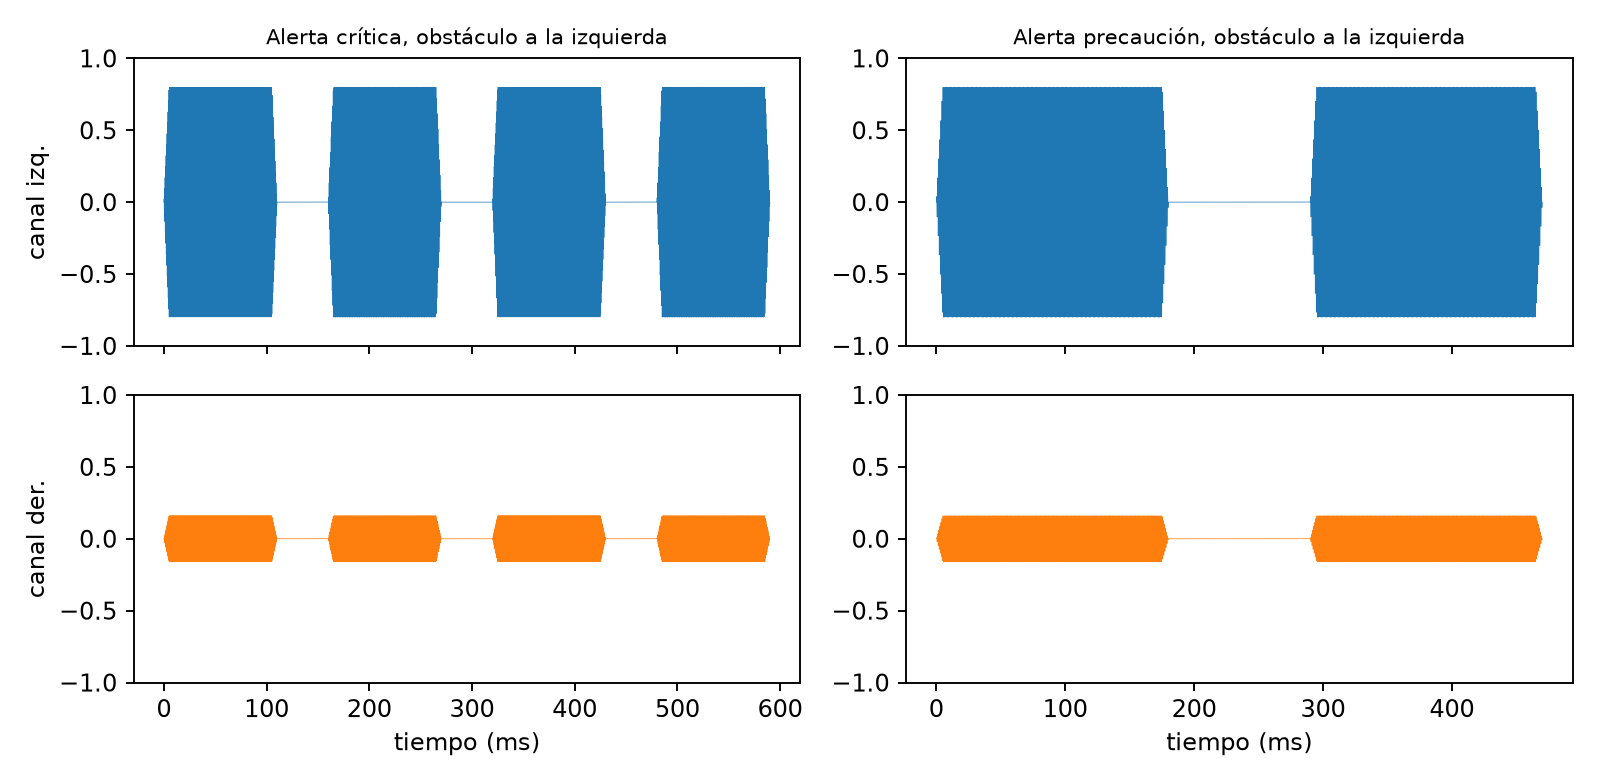
\includegraphics[width=0.88\textwidth]{Capturas_TT2/nav/alertas_pitidos.png}
    \caption{Forma de onda de los pitidos para un obstáculo a la izquierda, con la alerta
    crítica a la izquierda y la precaución a la derecha. El canal derecho suena al
    20\,\% del volumen del izquierdo.}
    \label{fig:alertas_pitidos}
\end{figure}

El módulo del equipo trae también su propia lógica para decidir el nivel; por ejemplo,
un vehículo a menos de 5~m es crítico, y si un sensor y la cámara reportan lo mismo en la
misma dirección casi al mismo tiempo, la alerta sube un nivel. En el sistema integrado
esa lógica no se usa, porque el nivel lo decide \texttt{alertas.py} con las reglas de la
Tabla~\ref{tab:alertas_reglas} y el módulo del equipo solo se encarga de sonar.

\subsection{Resultados}

\textbf{Pruebas con el prototipo.} \TODO{escenarios probados con el prototipo (por
ejemplo, acercarse a una pared, a una puerta de vidrio y a una persona), alertas
esperadas contra alertas emitidas, falsas alarmas y si los participantes distinguieron
la dirección de los pitidos}.

\textbf{Escenario simulado.} Para revisar el comportamiento de las reglas se preparó un
escenario en el cuarto simulado, en el que el usuario camina en línea recta hacia la
pared del fondo mientras una persona le cruza por delante. La
Figura~\ref{fig:alertas_escenario} muestra la distancia libre al frente según el mapa,
la distancia estimada a la persona y las alertas que emitió el módulo, 14 en total en
17~s.

\begin{figure}[H]
    \centering
    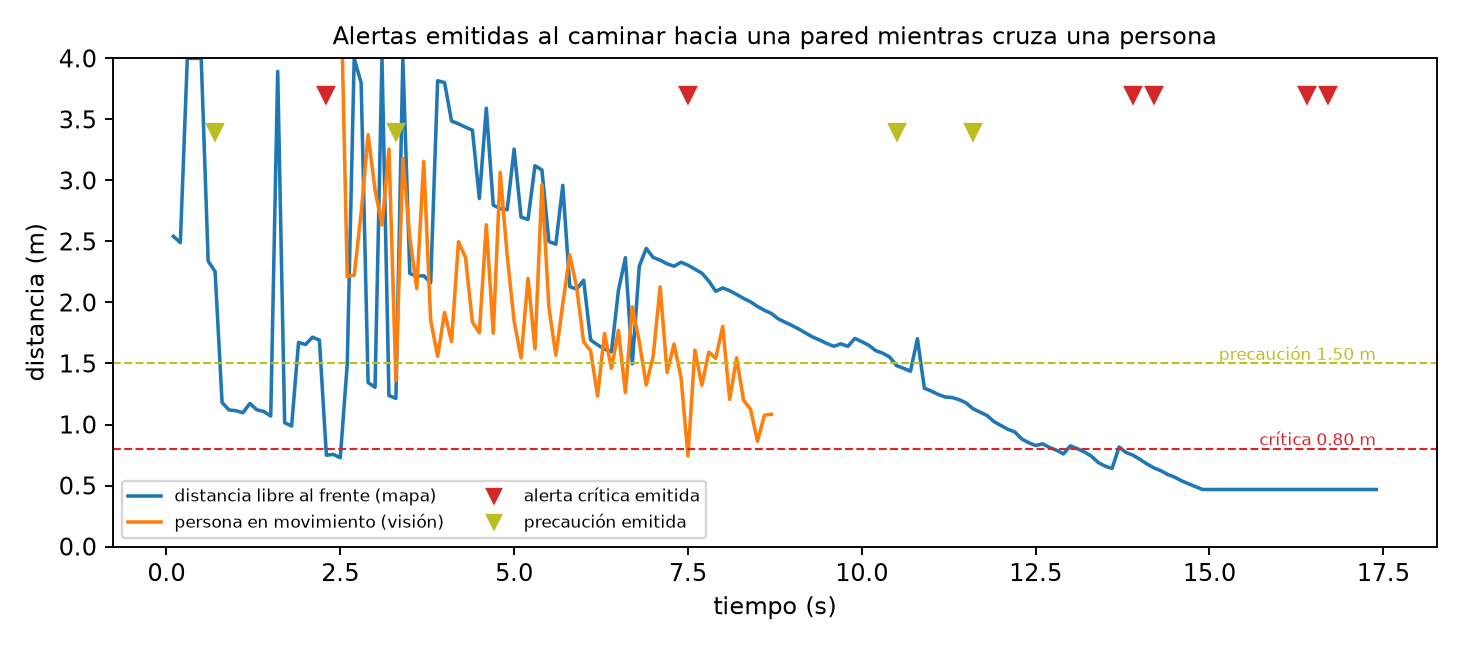
\includegraphics[width=\textwidth]{Capturas_TT2/nav/alertas_escenario.png}
    \caption{Alertas emitidas en el escenario de prueba. Los triángulos marcan cada alerta
    crítica (rojo) y cada precaución (verde).}
    \label{fig:alertas_escenario}
\end{figure}

La persona se avisó como se esperaba. A los 3.3~s, ya a menos de 2~m, sonó ``Precaución:
una persona en movimiento al frente'', y a los 7.5~s, a menos de 1~m, la alerta crítica
``Alto. Se acerca una persona al frente, muy cerca''. Al seguir su camino, la persona
quedó del lado derecho del usuario y el aviso cambió de dirección (8.5~s). Después el
ultrasonido detectó la pared, primero con precauciones a los 11.6 y 12.4~s y luego con
alertas críticas a los 13.9, 15.0 y 16.4~s, la última a 51~cm, porque el usuario siguió
avanzando. Entre los 12.6 y los 13.9~s el mapa ya marcaba menos de 0.80~m, pero el eco,
que mide la distancia real, todavía estaba por encima del umbral; como el aviso del
ultrasonido reemplaza al del mapa en esa dirección, la alerta crítica esperó a que el
eco bajara.

La prueba dejó ver dos efectos que conviene tener presentes. El primero es que el
cálculo estéreo del lado oscila cuando el usuario se acerca a una pared con un ligero
ángulo, de modo que la misma pared se reporta unas veces ``al frente'' y otras
``adelante a la derecha''. Como la dosificación cuenta cada dirección por separado, eso
produjo cinco avisos por la misma pared en menos de cinco segundos. \TODO{agrupar los
avisos del ultrasonido en una sola dirección frontal cuando ambos sensores ven la misma
superficie}. El segundo es que al inicio sonaron alertas por la mesa y el sillón que
quedaban a los lados, algunas con una distancia menor a la real. El escenario parte de un
mapa construido en un recorrido previo y la pose inicial se fijó a mano, así que hay un
desajuste entre la pose y el mapa; en una corrida de prueba se comprobó que, con la pose
desplazada 0.4~m, una pared ya registrada aparecía a 40~cm en un costado donde no había
nada.

En cuanto al tiempo, evaluar las reglas toma en promedio 0.007~ms por ciclo, así que lo
que tarda una alerta en sonar desde que el obstáculo aparece en la imagen depende de la
visión, unos 160~ms por cuadro en la computadora portátil. En el prototipo esa latencia
es de \TODO{latencia de alerta medida en la Raspberry Pi}, contra los 2~s que permite
RNF-01. El módulo tiene 26 pruebas automatizadas junto con el planificador de ruta.

\subsection{Limitaciones}

Las alertas heredan los errores de la percepción. Un tapete detectado como hoyo provoca
una alerta falsa, y un obstáculo que la cámara no reconoce y que no devuelve eco, como
un objeto bajo y muy cercano, no provoca ninguna. Tampoco hay alertas para lo que queda
detrás o muy a los costados del usuario, porque ni la cámara ni los ultrasónicos cubren
esas zonas.


% ==============================================================================
\section{Módulos de interacción: voz, PLN y salida}
\label{sec:dev_interaccion}
% ==============================================================================

\subsection{Descripción}

Los módulos de interacción son la única interfaz entre el usuario y el sistema. El
usuario habla, el sistema transcribe lo que dijo, interpreta la intención y responde
en voz alta; ninguna función requiere ver una pantalla ni tocar un botón, salvo el
botón opcional para apagar las alertas. Estos módulos atienden RF-01 a RF-06 y los
requerimientos no funcionales RNF-02, RNF-07, RNF-10 y RNF-11.

El reconocimiento de voz, el procesamiento de lenguaje natural (PLN), la personalidad
del asistente y la síntesis de voz los desarrolló el equipo en la carpeta
\texttt{VozYPLN/}. El trabajo de integración consistió en conectar esas piezas con el
navegador y con las alertas en \texttt{interaccion.py}. La Tabla~\ref{tab:inter_partes}
resume los componentes.

\begin{table}[H]
\centering
\caption{Componentes de los módulos de interacción}
\label{tab:inter_partes}
\renewcommand{\arraystretch}{1.25}
\begin{tabular}{|p{3.6cm}|p{10.9cm}|}
\hline
\textbf{Componente} & \textbf{Función} \\
\hline
\texttt{voz\_recog.py} & Reconocimiento de voz sin conexión con Vosk (modelo
\texttt{vosk-model-small-es-0.42}) a 16~kHz. \\
\hline
\texttt{PLN\_oneimport.py} & Clasificación de la intención y extracción del destino. \\
\hline
\texttt{dialogo.py} & Frases con la personalidad del asistente (``Guía''). \\
\hline
\texttt{Tts.py} & Síntesis de voz con edge-tts (voz \texttt{es-MX-DaliaNeural}) y respaldo
local con pyttsx3. \\
\hline
\texttt{interaccion.py} & Integración: cola de voz con prioridades, escucha en segundo
plano y traducción de intenciones a comandos del navegador. \\
\hline
\end{tabular}
\end{table}

Respecto al diseño de TT1 hubo tres cambios. El detector de actividad de voz y el
filtro de Wiener que se habían planteado como etapas previas no se implementaron por
separado: Vosk detecta por sí mismo el final de cada frase y el filtro no mejoró el
reconocimiento en las primeras pruebas. El PLN no usa spaCy, sino un clasificador
propio escrito en Python puro, que combina reglas con una red neuronal pequeña. Y la
síntesis de voz usa una voz neuronal en línea con un respaldo local, en lugar de
depender solo de pyttsx3.

\subsection{Reconocimiento de voz}

El reconocedor captura audio del micrófono en bloques de 0.25~s y los entrega a Vosk.
Cuando Vosk detecta que la frase terminó, devuelve el texto y el reconocedor lo coloca
en una cola que el ciclo principal revisa en cada cuadro. La escucha corre en un hilo
aparte, de modo que el sistema sigue percibiendo y navegando mientras espera una
orden. Mientras el sistema habla, lo que capta el micrófono se descarta, porque lo más
probable es que se esté escuchando a sí mismo. Si no hay micrófono o falta el modelo de
Vosk, el sistema lo avisa y acepta las órdenes por teclado, lo cual se usa durante el
desarrollo.

\subsection{Procesamiento de lenguaje natural}

El PLN recibe el texto transcrito y devuelve una de 14 intenciones, el destino si lo
hay, un valor de confianza y una respuesta sugerida. Las intenciones son: destino,
pausa, reanudar, detener, ruta alternativa, emergencia, ubicación, entorno, repetir,
cancelar, ayuda, confirmar, negar y estado de la ruta. El proceso tiene cuatro pasos:

\begin{enumerate}
    \item \textbf{Normalización.} El texto se pasa a minúsculas, se quitan los acentos
    y los signos, y se divide en palabras. Se descartan palabras sin contenido (``el'',
    ``por favor'') y se agregan sinónimos conocidos.
    \item \textbf{Palabras de seguridad.} Si el texto contiene una palabra como
    ``detente'', ``alto'', ``auxilio'' o ``cancela'', la intención se fija de inmediato
    con confianza de 0.99, sin consultar a los clasificadores.
    \item \textbf{Clasificación.} Se calculan dos puntuaciones para cada intención. La
    de reglas compara el texto con 121 frases de referencia mediante similitud de
    palabras basada en la distancia de Levenshtein, que tolera errores del
    reconocedor, y similitud de coseno entre bolsas de palabras. La de la red neuronal
    usa una capa oculta de 24 neuronas sobre un vector TF-IDF, entrenada con 164
    ejemplos (las frases de referencia más variantes con sinónimos). Ambas se combinan
    con un peso para la red que crece con el número de ejemplos aprendidos y con la
    proporción de palabras del texto que la red conoce. Si la mejor puntuación es
    menor que 0.42, o si las dos mejores quedan casi empatadas, el resultado es
    ``desconocido'' y el sistema pide repetir.
    \item \textbf{Destino.} Para la intención de destino se busca primero un lugar
    conocido por similitud, después lo que sigue a frases como ``llévame a'' o
    ``quiero ir a'' y, como último recurso, las palabras que quedan al quitar las de
    navegación. Si no hay destino, el sistema pregunta ``¿A dónde te gustaría ir?'' y
    toma la siguiente frase como respuesta.
\end{enumerate}

El PLN puede aprender frases nuevas cuando recibe una corrección, y las guarda en un
archivo local. Para la evaluación de esta sección se usó el modelo sin frases
aprendidas, que es el que tendría un usuario nuevo.

\subsection{Integración con el navegador}

La clase \texttt{Interaccion} convierte cada intención en una acción. Las de la
sesión (destino, pausa, reanudar, detener, cancelar, ruta alternativa, ubicación y
estado) se envían al navegador como comandos. El destino se limpia antes de enviarlo
(se quitan artículos y plurales, porque el PLN puede devolver ``la puerta'' o
``baños'') y se traduce a la etiqueta del \emph{landmark} con un diccionario de
sinónimos: ``salida'', ``puerta'' y ``entrada'' se buscan como \emph{door}; ``baño''
como \emph{toilet}; ``escritorio'' como \emph{desk}, y así para 38 palabras. Las demás
intenciones se resuelven en la misma clase:

\begin{itemize}
    \item \textbf{Entorno} (``¿qué hay enfrente?''): describe el objeto más cercano en
    cada sector, o la distancia libre si no hay ninguno. La frase tiene la forma ``Al
    frente, door a 2 metros. A la izquierda libre. A la derecha, chair a 90
    centímetros'': el nombre del objeto se dice con la etiqueta en inglés del
    detector, lo cual es una deficiencia pendiente.
    \item \textbf{Repetir}: vuelve a decir la última indicación de navegación.
    \item \textbf{Emergencia}: emite un aviso con prioridad máxima y pausa la
    navegación. El aviso a un contacto de emergencia quedó pendiente.
    \item \textbf{Ayuda}: enumera lo que se puede decir.
\end{itemize}

Las frases ``apagar sistema'' y ``terminar programa'' cierran el sistema con una
despedida.

\subsection{Salida de voz}

Todo lo que el sistema dice pasa por una cola con tres prioridades: 0 para alertas, 1
para indicaciones de navegación y 2 para respuestas y confirmaciones. Un mensaje de
prioridad 0 interrumpe lo que se esté diciendo. Las indicaciones de navegación forman
un canal especial en el que solo se dice la más reciente: si el sintetizador va
atrasado y en la cola hay un ``gire a la izquierda'' viejo, se descarta, porque ya no
corresponde a la posición del usuario; también se descartan las indicaciones que
llevan más de 6~s esperando. Mientras suena un pitido de alerta, la cola espera.

La síntesis usa edge-tts con la voz neuronal \texttt{es-MX-DaliaNeural}, que suena
natural pero necesita conexión a internet. Cada frase sintetizada se guarda en un
archivo, así que las frases repetidas (que son la mayoría) se reproducen sin conexión.
Si la conexión falla, el sistema cambia a pyttsx3, que usa la voz instalada en el
sistema operativo; si tampoco está disponible, escribe las frases en consola.

\subsection{Personalidad del asistente}

El navegador genera las frases literales definidas en TT1 (``Avance 3 metros'',
``Gire ligeramente a la izquierda''). Con el modo amigable activado, que es el
predeterminado, \texttt{dialogo.py} las reformula con un tono más cercano: la
distancia se expresa en pasos, los giros con referencias cotidianas y las frases
varían para no sonar repetitivas (Tabla~\ref{tab:inter_frases}). La frase
``Deténgase'' y las alertas no se reformulan, porque en esos casos importa más la
rapidez que la amabilidad.

\begin{table}[H]
\centering
\caption{Frases literales del navegador y su versión amigable}
\label{tab:inter_frases}
\renewcommand{\arraystretch}{1.25}
\begin{tabular}{|p{5.2cm}|p{9.3cm}|}
\hline
\textbf{Literal (TT1)} & \textbf{Amigable (dialogo.py)} \\
\hline
Ruta calculada. Iniciando navegación. & Muy bien, te llevo a sillon. Vamos paso a
paso. \\
\hline
Gire ligeramente a la izquierda & Perfecto, da una vuelta suave a tu izquierda. \\
\hline
Gire a la derecha 90 grados & Listo, da vuelta completa a tu derecha, como una
esquina. \\
\hline
Avance 3 metros & Vas muy bien, continúa de frente unos 4 pasos. \\
\hline
Ha llegado a su destino. & ¡Listo, llegamos a door! \\
\hline
Deténgase & Deténgase (sin cambio) \\
\hline
\end{tabular}
\end{table}

Una sutileza de la integración: \texttt{dialogo.py} considera positivos los giros a la
derecha, mientras que en el resto del sistema los ángulos positivos son hacia la
izquierda. La conversión invierte el signo; las pruebas automatizadas verifican que
un giro a la izquierda del navegador se diga ``a tu izquierda''.

El Algoritmo~\ref{alg:dev_inter} resume el manejo de una frase del usuario.

\begin{center}
\captionof{algorithm}{Manejo de una frase del usuario}
\label{alg:dev_inter}
\end{center}
\vspace{-1.8cm}
\rule{\textwidth}{0.4pt}
\vspace{-0.9cm}
\begin{algorithmic}[1]

\Statex \textbf{ENTRADA:} texto (de Vosk o del teclado), cuadro\_nav
\Statex \textbf{SALIDA:} mensajes para la cola de voz

\Statex
\If{texto es ``apagar sistema'' o ``terminar programa''}
    \State \Return [despedida]
\EndIf
\If{se esperaba la respuesta a ``¿a dónde te gustaría ir?''}
    \State texto $\gets$ ``llévame a '' + texto
\EndIf
\State r $\gets$ PLN.procesar(texto)
\If{r.intención = destino}
    \If{no hay destino}
        \State marcar que se espera respuesta
        \State \Return [``¿A dónde te gustaría ir?'']
    \EndIf
    \State etiqueta $\gets$ sinónimos(limpiar(r.destino))
    \State msgs $\gets$ navegador.comando(navegar, etiqueta, cuadro\_nav)
\ElsIf{r.intención es de sesión}
    \State msgs $\gets$ navegador.comando(r.intención)
\ElsIf{r.intención = entorno}
    \State msgs $\gets$ [describir\_entorno(cuadro\_nav)]
\ElsIf{r.intención = emergencia}
    \State msgs $\gets$ [aviso con prioridad 0] + navegador.comando(pausa)
\Else
    \State msgs $\gets$ [respuesta según la intención]
\EndIf
\If{modo amigable}
    \State reformular las confirmaciones con dialogo.py
\EndIf
\State \Return msgs

\end{algorithmic}
\vspace{-0.9cm}
\rule{\textwidth}{0.4pt}

\subsection{Resultados}

\textbf{Evaluación del PLN.} Para medir el PLN con frases que no conociera, se
redactó un conjunto de 102 frases de prueba, distintas de las frases de referencia,
con la intención correcta de cada una (por ejemplo, ``espérame tantito'' para pausa o
``ya no quiero seguir'' para detener). El conjunto se escribió antes de correr la
evaluación y no se modificó después de ver los resultados. El PLN acertó la intención
en 80 de las 102 frases (78.4\,\%). En las frases de destino, extrajo correctamente
el lugar en 16 de 21. Procesar una frase tomó en promedio 2.8~ms (máximo 7~ms). La
Figura~\ref{fig:pln_confusion} muestra la matriz de confusión.

\begin{figure}[H]
    \centering
    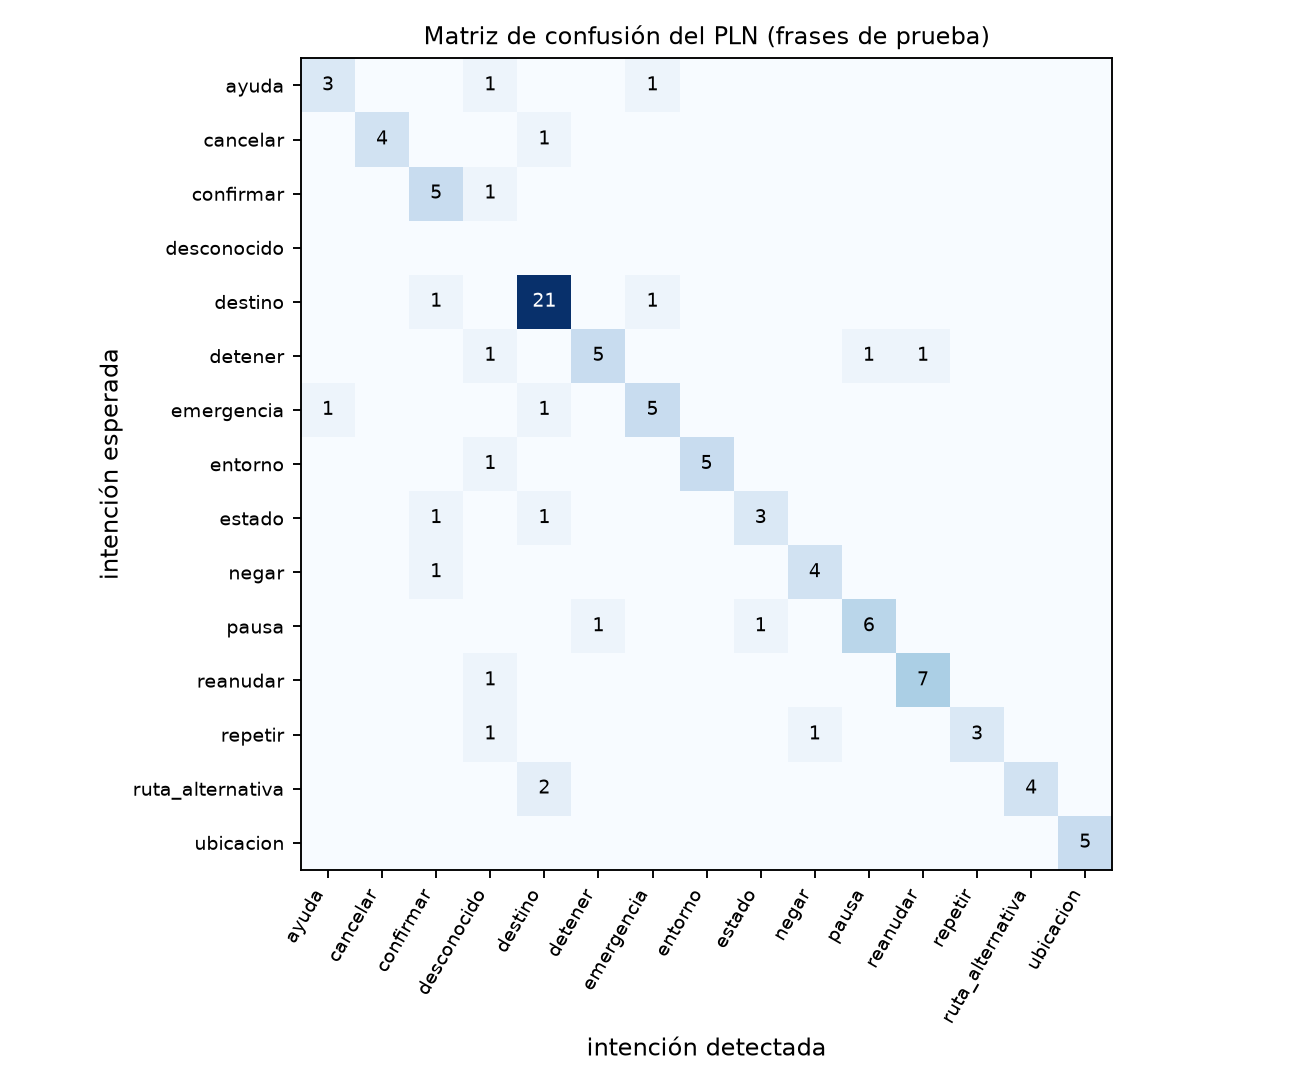
\includegraphics[width=0.78\textwidth]{Capturas_TT2/voz/pln_confusion.png}
    \caption{Matriz de confusión del PLN sobre las 102 frases de prueba.}
    \label{fig:pln_confusion}
\end{figure}

La mayoría de los errores son inofensivos: la frase cae en ``desconocido'' y el
sistema pide repetir, o el destino se extrae con palabras de sobra (``llevas banca'',
``guiar mesa''), lo que hace que no se encuentre el lugar. Algunos, sin embargo, son
delicados por su efecto sobre la navegación:

\begin{itemize}
    \item ``ya no quiero seguir'' se interpretó como reanudar, y ``termina la
    navegación'' como pausa;
    \item ``no es correcto'' se interpretó como confirmar;
    \item ``ayuda'' se interpretó como emergencia y, al revés, ``ayuda, me caí'' como
    una petición de ayuda sobre los comandos;
    \item ``detente un momento por favor'' se interpretó como detener en lugar de
    pausa, por la palabra de seguridad ``detente''. Esta última es una decisión de
    diseño conservadora y se considera aceptable.
\end{itemize}

\textbf{Reconocimiento de voz con ruido.} Para evaluar la cadena completa sin
voluntarios se generó audio con las 10 voces en español disponibles en macOS (dos
voces naturales, Paulina y Mónica, y ocho voces de estilo caricaturesco) diciendo 30
comandos de uso frecuente. Cada audio se pasó por Vosk y por el PLN en limpio y
mezclado con ruido rosa a 20, 10 y 5~dB de relación señal a ruido. Un comando cuenta
como correcto si produce la acción esperada y, en los de destino, el lugar correcto.
Los resultados se muestran en la Tabla~\ref{tab:asr} y en la
Figura~\ref{fig:asr_ruido}.

\begin{table}[H]
\centering
\caption{Voz sintetizada, Vosk y PLN (300 audios por condición)}
\label{tab:asr}
\renewcommand{\arraystretch}{1.2}
\begin{tabular}{|l|c|c|c|}
\hline
\textbf{Condición} & \textbf{WER} & \textbf{Comandos correctos} &
\textbf{Correctos, voces naturales} \\
\hline
Limpio & 22.2\,\% & 80.0\,\% & 91.7\,\% \\
20~dB & 23.8\,\% & 78.3\,\% & 81.7\,\% \\
10~dB & 33.0\,\% & 71.0\,\% & 63.3\,\% \\
5~dB & 43.1\,\% & 58.7\,\% & 45.0\,\% \\
\hline
\end{tabular}
\end{table}

\begin{figure}[H]
    \centering
    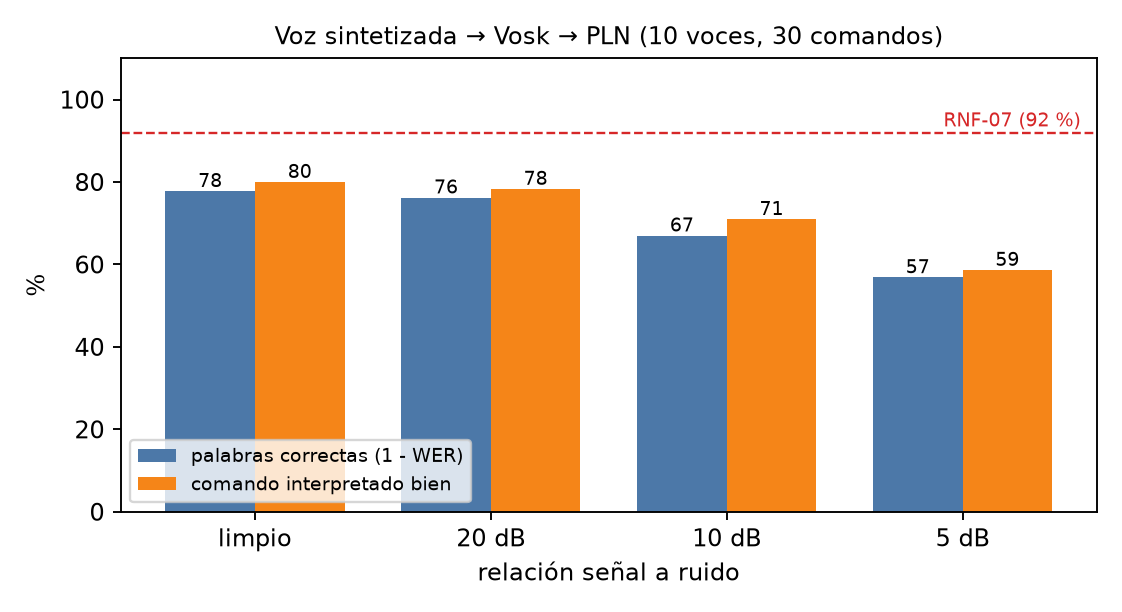
\includegraphics[width=0.75\textwidth]{Capturas_TT2/voz/asr_ruido.png}
    \caption{Palabras correctas y comandos bien interpretados según el nivel de ruido.}
    \label{fig:asr_ruido}
\end{figure}

En audio limpio con las voces naturales el sistema interpreta bien el 91.7\,\% de los
comandos, prácticamente en el 92\,\% que pide RNF-07. Con ruido el desempeño cae
rápido. Una voz hablada a corta distancia del micrófono en un entorno de 60~dB
(el nivel que menciona RNF-07) equivale aproximadamente a la franja de 5 a 10~dB de la
tabla, donde los comandos correctos están entre 59 y 71\,\%. Por lo tanto, el
requerimiento no se cumple en condiciones ruidosas. También se observó que, en los
194 audios limpios que Vosk transcribió sin ningún error, el PLN acertó en 181
(93\,\%); el resto del error en limpio proviene del reconocimiento.

En cuanto a la latencia, una vez que termina el audio Vosk entrega el resultado final
en 8~ms en promedio (17~ms en el percentil 95) y el PLN tarda 2~ms. Esta medición no
incluye el tiempo que Vosk espera en silencio para decidir que la frase terminó,
que en uso real se suma a la latencia percibida. Aun así, el procesamiento queda muy
por debajo de los 500~ms de RNF-02.

Las pruebas automatizadas de la interacción (24) verifican la traducción de
intenciones a comandos, la aclaración de destino en dos turnos, la limpieza de
destinos, la conversión de signo de los giros, la descripción del entorno y el
funcionamiento sin micrófono ni sintetizador.

\subsection{Limitaciones}

\begin{itemize}
    \item El PLN acierta el 78\,\% de las frases nuevas y comete errores que invierten el
    sentido de la orden (detener interpretado como reanudar). Ampliar las frases de
    referencia con las formas que usan las personas y revisar las palabras de seguridad
    son los pasos inmediatos.
    \item Con ruido de calle, el reconocimiento queda lejos del 92\,\% de RNF-07.
    \item La evaluación de voz usó voces sintéticas; falta probar con personas reales,
    con distintos acentos y con el micrófono del prototipo.
    \item La voz neuronal requiere internet la primera vez que se dice cada frase; sin
    conexión se usa una voz del sistema mucho menos natural.
    \item La llegada y la descripción del entorno mencionan las etiquetas en inglés
    del detector (``llegamos a door'', ``chair a 90 centímetros''). Hace falta un
    diccionario inverso de etiquetas a nombres en español.
    \item El aviso a un contacto de emergencia no está implementado.
\end{itemize}





% Conclusiones de TT1 (escritas antes del desarrollo); las sustituye el capítulo
% de resultados y conclusiones de TT2. Se conserva el archivo por si se requiere.
% \chapter{Trabajo a futuro y Conclusiones}

Durante TT2 se continuará con la fase de desarrollo e implementación del proyecto, tomando como base la investigación, documentación y análisis realizados previamente.

Como parte del trabajo futuro, se desarrollará la integración del sistema, basado en diagramas de arquitectura, diseño de módulos, flujo de procesamiento de datos e integración para la interacción entre componentes de hardware y software.

Se realizará la implementación progresiva de los módulos previamente investigados, integrando sistemas de visión computacional, reconocimiento de voz, navegación y generación de instrucciones auditivas dentro de una plataforma funcional.

Asimismo, se llevará a cabo el entrenamiento y ajuste de los modelos de inteligencia artificial mediante pruebas controladas y recopilación de datos en escenarios representativos, permitiendo evaluar el comportamiento del sistema ante distintos tipos de obstáculos y condiciones ambientales.

También se documentarán las pruebas experimentales realizadas al prototipo, registrando métricas de desempeño relacionadas con precisión de detección, tiempos de respuesta, estabilidad operativa y efectividad de navegación.

Durante esta etapa se buscará validar el funcionamiento integral del sistema mediante pruebas en entornos interiores y exteriores, analizando la capacidad del prototipo para asistir al usuario durante recorridos básicos de navegación.

Adicionalmente, se contempla continuar investigando estrategias de optimización orientadas a mejorar la eficiencia del procesamiento en hardware embebido, así como técnicas de navegación adaptativa y recalculación de rutas en tiempo real.

Como objetivo principal, se busca obtener un prototipo funcional y documentado que permita validar la propuesta tecnológica planteada en la etapa de investigación, demostrando la factibilidad del sistema como herramienta de asistencia para personas con visión reducida.

\section{Conclusiones de Trabajo Terminal I}
A partir de la investigación y análisis realizados durante TT1, se determinó la viabilidad técnica del desarrollo de un sistema de navegación asistida para personas con visión reducida, integrando tecnologías de inteligencia artificial, visión computacional y procesamiento de voz.

La etapa de investigación permitió identificar los principales desafíos asociados a la movilidad autónoma asistida, así como las tecnologías más adecuadas para abordar problemas relacionados con detección de obstáculos, orientación espacial y emisión de instrucciones auditivas en tiempo real.

Se estableció una arquitectura modular para el sistema, permitiendo definir de manera estructurada cada uno de los componentes que conformarán el prototipo funcional en TT2. Esta arquitectura facilita la documentación, validación e integración progresiva de los módulos de hardware y software.

Asimismo, se definieron los requerimientos funcionales y no funcionales del sistema, considerando aspectos fundamentales como precisión, latencia, autonomía operativa y capacidad de procesamiento en una raspberry pi.

La investigación tecnológica realizada permitió justificar el uso de herramientas como YOLOv8 para detección de objetos, Vosk para reconocimiento de voz, spaCy para procesamiento de lenguaje natural y algoritmos de navegación basados en SLAM y aprendizaje profundo por refuerzo, debido a su compatibilidad con entornos de tiempo real y hardware de recursos limitados.

De igual manera, se documentaron los flujos operativos, casos de uso, interacciones del sistema y posibles escenarios de funcionamiento, estableciendo una base sólida para el desarrollo e implementación del prototipo durante la siguiente etapa del proyecto terminal.

Finalmente, el proyecto se sustenta en una problemática social relevante, orientada a generar herramientas tecnológicas de apoyo que contribuyan a mejorar la autonomía y seguridad de las personas con discapacidad visual durante sus desplazamientos.



% Secciones finales TT 2
\chapter{Resultados y conclusiones}
\label{cap:conclusiones}

En este capítulo se juntan los resultados de Trabajo Terminal II, se comparan con los
objetivos y requerimientos planteados en TT1 y se presentan las conclusiones del
trabajo. El detalle de cada medición está en el Capítulo~\ref{cap:desarrollo}.

% ==============================================================================
\section{Resumen de resultados}
% ==============================================================================

La Tabla~\ref{tab:resumen_resultados} resume el resultado principal de cada módulo y
las condiciones en las que se obtuvo.

\begin{longtable}{|p{2.6cm}|p{6.4cm}|p{5.5cm}|}
\caption{Resultados principales por módulo}
\label{tab:resumen_resultados} \\
\hline
\textbf{Módulo} & \textbf{Resultado} & \textbf{Condición de la prueba} \\
\hline
\endfirsthead
\hline
\textbf{Módulo} & \textbf{Resultado} & \textbf{Condición de la prueba} \\
\hline
\endhead
Prototipo & \TODO{resultado general de los recorridos con el prototipo} &
\TODO{lugares, participantes y número de recorridos} \\
\hline
Visión & Detecta personas, muebles, puertas con su estado, escaleras y peligros de piso,
en unos 160~ms por cuadro. & 19 videos reales, CPU de computadora portátil;
\TODO{precisión en imágenes etiquetadas del prototipo}. \\
\hline
SLAM & ATE de 0.21~m en recorridos cortos; con odometría sesgada, el error queda entre
la mitad y tres cuartas partes del de la odometría sola. & Banco de simulación, seis
semillas. \\
\hline
Ray Casting & Actualización y consulta del mapa en menos de 1~ms por ciclo. &
Simulación y videos reales. \\
\hline
Mapeo & Mapa por bloques con persistencia; 19 mapas de lugares reales de entre 24 y
60~KB. & Videos reales. \\
\hline
Navegación & 97.8\,\% de llegadas, 2.0\,\% de choques y ninguna caída en 880
episodios. & Simulador de entrenamiento con 19 mapas reales. \\
\hline
Navegación (sistema completo) & 20 de 20 sesiones con llegada; en 17 el usuario terminó
a menos de 1~m del objeto. & Lazo cerrado con todos los módulos y un usuario
virtual. \\
\hline
Alertas & Avisos críticos y de precaución con pitido estéreo; evaluación en 0.007~ms
por ciclo. & Escenario simulado con una persona cruzando. \\
\hline
PLN & 51.2\,\% de intenciones correctas en 86 frases coloquiales que el PLN no conocía,
en 4.8~ms por frase. & Frases redactadas antes de la evaluación y fuera del conjunto de
referencia. \\
\hline
Voz completa & 95.0\,\% de comandos correctos en limpio con voces naturales, y de 62 a
74\,\% con ruido de 5 a 10~dB. & Voz sintetizada, Vosk y PLN;
\TODO{resultado con personas y el micrófono del prototipo}. \\
\hline
\end{longtable}

% ==============================================================================
\section{Cumplimiento de los objetivos}
% ==============================================================================

\textbf{Objetivo general.} Se desarrolló un sistema de navegación asistida montado en
unos lentes, que combina visión artificial, localización y mapeo simultáneos, trazado de
rayos, aprendizaje por refuerzo e interacción por voz. El sistema funciona de principio a
fin en el prototipo, y el mismo código corre en una computadora portátil con cámara,
con videos grabados y en simulación. \TODO{resumen de cómo se comportó el prototipo en
las pruebas con personas y si se considera cumplido el objetivo general}.

\textbf{Objetivo 1, modelo de visión con precisión mayor al 80\,\%.} Se integraron tres
modelos que detectan y segmentan los objetos relevantes, incluidas las puertas, que el
detector original no reconocía. Las pruebas con video mostraron también sus errores
típicos, como confundir mamparas con puertas o tapetes con hoyos. \TODO{precisión medida
en imágenes etiquetadas del prototipo y veredicto sobre el 80\,\%}.

\textbf{Objetivo 2, reconstrucción del escenario con trazado de rayos.} El mapa del
entorno se construye con Ray Casting sobre una retícula de ocupación, se divide en
bloques, se guarda entre sesiones y se consulta para obtener las distancias que usa la
navegación. Se eligió Ray Casting en lugar de un trazado de rayos completo por su costo,
como se justificó en el marco teórico. El mapa también se corrige cuando el entorno
cambia, porque los ecos precisos liberan las celdas de un obstáculo que se retiró y la
segmentación borra los falsos peligros de piso. El objetivo se cumple.

\textbf{Objetivo 3, navegación con una medición del terreno 90\,\% segura.} En el
simulador, el agente llegó a la meta en el 97.8\,\% de los episodios, chocó en el
2.0\,\% y nunca cayó en un peligro de piso. Con el sistema completo en lazo cerrado,
el usuario virtual llegó en las 20 sesiones y en 17 terminó a menos de un metro del
objeto. Tomando como medida de seguridad la tasa de episodios sin choque ni caída, el
objetivo se cumple en simulación. \TODO{tasa de recorridos seguros con el prototipo y
veredicto sobre el 90\,\%}.

\textbf{Objetivo 4, interacción por voz.} El sistema reconoce comandos de voz sin
conexión, responde en voz alta con una voz natural y se puede usar sin pantalla. El
objetivo se cumple; su punto débil es el desempeño con ruido.

\textbf{Objetivo 5, lenguaje natural para indicaciones cotidianas y de emergencia.}
El PLN reconoce 14 intenciones, entre ellas la emergencia, y la personalidad del
asistente hace que las indicaciones suenen cercanas, con los objetos nombrados en
español. Los comandos de uso frecuente se interpretan bien, pero con frases coloquiales
que no conoce el PLN acierta poco más de la mitad, y algunas emergencias dichas sin
palabras de lesión no se reconocen, así que el objetivo se cumple en parte. \TODO{aviso
a contactos de emergencia}.

% ==============================================================================
\section{Cumplimiento de los requerimientos}
% ==============================================================================

La Tabla~\ref{tab:cumplimiento_req} muestra el estado de cada requerimiento. ``Parcial''
quiere decir que la función existe pero con una limitación medida.

\begin{longtable}{|p{1.6cm}|p{4.6cm}|p{1.9cm}|p{6.4cm}|}
\caption{Estado de los requerimientos funcionales y no funcionales}
\label{tab:cumplimiento_req} \\
\hline
\textbf{Req.} & \textbf{Descripción} & \textbf{Estado} & \textbf{Observación} \\
\hline
\endfirsthead
\hline
\textbf{Req.} & \textbf{Descripción} & \textbf{Estado} & \textbf{Observación} \\
\hline
\endhead
RF-01 & Captura de voz con detección de actividad & Cumplido & Vosk detecta el fin
de cada frase. \\
\hline
RF-02 & Filtrado de audio & No implementado & El filtro de Wiener no mostró mejora y
se dejó fuera. \\
\hline
RF-03 & Reconocimiento e intención & Parcial & 95\,\% de los comandos frecuentes en
limpio, pero 51.2\,\% en frases coloquiales nuevas. \\
\hline
RF-04 & Síntesis de voz & Cumplido & Voz neuronal con respaldo local. \\
\hline
RF-05 & Control de sesión por voz & Cumplido & Iniciar, pausar, reanudar y
detener. \\
\hline
RF-06 & Todas las funciones por voz & Parcial & Las alertas se apagan con tecla o
botón, no por voz. \\
\hline
RF-07 & Captura y preprocesamiento & Parcial & Solo redimensionamiento; los demás
pasos se descartaron. \\
\hline
RF-08 & Detección con localización & Cumplido & Personas, obstáculos, puertas,
escaleras y desniveles. \\
\hline
RF-09 & Clasificación y riesgo & Cumplido & Riesgo de 0 a 3 según la tabla de TT1. \\
\hline
RF-10 & Distancia a los objetos & Cumplido & Monocular, con errores de 25\,\% o más,
y precisa con el ultrasonido dentro de su cono. \\
\hline
RF-11 & Validación con sensores & Cumplido & Validación cruzada con los dos
ultrasónicos frontales. \\
\hline
RF-12 & Alerta de obstáculo & Cumplido & Pitido estéreo y frase corta. \\
\hline
RF-13 & Relaciones contextuales & Parcial & Estado de las puertas, corregido con el
ultrasonido; no se mide la obstrucción de pasillos. \\
\hline
RF-14 & Estimación de la pose & Cumplido & EKF con IMU y respaldo por flujo
óptico. \\
\hline
RF-15 & Mapa incremental & Cumplido & Sin mapa previo. \\
\hline
RF-16 & Zonas libres y ocupadas & Cumplido & Log-odds y capa de peligros. \\
\hline
RF-17 & Actualización dinámica & Cumplido & Los ecos precisos liberan las celdas de
obstáculos retirados. \\
\hline
RF-18 & Ruta local & Cumplido & Agente de PPO y planificador. \\
\hline
RF-19 & Actualización periódica de la ruta & Cumplido & Cada 2~s. \\
\hline
RF-20 & Recálculo ante obstáculos & Cumplido & Decisión inmediata ante una alerta
crítica. \\
\hline
RF-21 & Instrucciones de movimiento & Cumplido & Frases de TT1 y versión
amigable. \\
\hline
RF-22 & Destinos sobre el mapa & Cumplido & Por etiqueta de \emph{landmark}. \\
\hline
RF-23 & Ruta alternativa por voz & Cumplido & Bloquea por tres minutos el tramo
siguiente y replanea; avisa si no hay otra ruta. \\
\hline
RNF-01 & Alerta en menos de 2~s & \TODO{} & Unos 160~ms en la computadora portátil;
\TODO{latencia en la Raspberry Pi}. \\
\hline
RNF-02 & Voz en menos de 500~ms & Cumplido & 10~ms de procesamiento, sin contar la
espera de fin de frase. \\
\hline
RNF-03 & Mapa a 10~Hz & \TODO{} & 1~ms por ciclo para la representación;
\TODO{frecuencia del ciclo completo en la Raspberry Pi}. \\
\hline
RNF-04 & Ruta cada 10~s o menos & Cumplido & Cada 2~s. \\
\hline
RNF-05 & Hardware limitado & \TODO{} & Inferencia de navegación en NumPy;
\TODO{uso de CPU y memoria en la Raspberry Pi}. \\
\hline
RNF-06 & Precisión de detección del 90\,\% & \TODO{} & \TODO{precisión medida}. \\
\hline
RNF-07 & 92\,\% de comandos con 60~dB & No cumplido & 95.0\,\% en limpio y de 62 a
74\,\% con ruido. \\
\hline
RNF-08 & Degradación controlada & Cumplido & Respaldos sin IMU, sin micrófono, sin
voz y sin internet. \\
\hline
RNF-09 & Comportamiento conservador & Cumplido & Capa de seguridad, confianza de la
pose y alertas ``posible'' para detecciones contradichas. \\
\hline
RNF-10 & Interfaz solo por voz & Parcial & Igual que RF-06. \\
\hline
RNF-11 & Instrucciones claras & Cumplido & Frases cortas en español, distancias en
pasos y objetos con su nombre en español. \\
\hline
RNF-12 & Retroalimentación proactiva & Cumplido & Alertas, llegada y cambios de
zona. \\
\hline
RNF-13 & Operación sin internet & Cumplido & Con una voz de respaldo menos
natural. \\
\hline
RNF-14 & Modularidad & Cumplido & Interfaces comunes; el mismo código trabaja con
cámara, video y simulación. \\
\hline
RNF-15 & Actualización de modelos & Cumplido & Modelos intercambiables y script de
reentrenamiento. \\
\hline
\end{longtable}

% ==============================================================================
\section{Conclusiones}
% ==============================================================================

Al terminar TT1, la propuesta era una arquitectura en papel. Al terminar TT2 hay unos
lentes que reciben la imagen de una cámara, entienden una orden hablada, construyen un
mapa del lugar, deciden por dónde ir y lo dicen en voz alta, con todos los módulos
conectados y probados. Ese es el resultado principal del trabajo.

La lección técnica más importante tiene que ver con la forma de evaluar. Varios módulos
parecían terminados hasta que se midieron dentro del sistema completo. El agente de
navegación llega al 97.8\,\% de las metas en su simulador, pero al trabajar junto con el
SLAM y la estimación monocular apareció un problema que solo se nota con todo integrado,
porque la regla de llegada por percepción terminaba las sesiones antes de tiempo. Medir
el sistema en lazo cerrado permitió encontrar la causa, corregirla y pasar de 7 a 17
sesiones de 20 con el usuario a menos de un metro del objeto. Algo parecido pasó con el
EKF, que apenas mejora a la odometría en recorridos cortos y muestra su valor cuando la
odometría tiene sesgo, y con el PLN, que acierta casi siempre las frases parecidas a
las suyas y apenas la mitad de las expresiones coloquiales que nunca vio. Ninguno de estos
hallazgos se habría visto midiendo cada módulo por separado.

La segunda conclusión es que la percepción manda sobre el resto. El mapa, la navegación
y las alertas tardan alrededor de un milisegundo por ciclo, mientras que la visión tarda
más de cien, y con los errores pasa algo similar; una distancia monocular equivocada o un
tapete tomado por hoyo se propagan hasta lo que escucha el usuario. Por eso las mejoras
con más impacto son de percepción, como reentrenar el detector con imágenes del entorno
real o separar la banqueta del arroyo vehicular. En esa misma línea, poner los
ultrasónicos al frente resultó una buena decisión, porque permiten confirmar lo que ve la
cámara, detectar vidrios y mamparas y dar por buena una llegada solo cuando la distancia
está verificada.

La tercera es que vale la pena mantener capas determinísticas por encima de los modelos
aprendidos. La capa de seguridad del navegador, las palabras de seguridad del PLN y el
módulo de alertas siempre encendido no dependen de que una red neuronal acierte. Aun así,
las pruebas mostraron sus límites; en una de las primeras sesiones, un objeto bajo y muy cercano
quedó fuera de la vista de todos los sensores y el sistema siguió indicando avanzar. Para
un sistema que guía a una persona con discapacidad visual, esa redundancia es necesaria,
y también lo es reconocer qué casos no cubre.

Por último, el sistema es un prototipo de investigación, que es el alcance definido para
este trabajo. \TODO{conclusión a partir de las pruebas con el prototipo y de la opinión
de los participantes}. Como se estableció en las limitaciones del proyecto, los lentes
son un complemento del bastón blanco y no lo sustituyen.

% ==============================================================================
\section{Trabajo a futuro}
\label{sec:trabajo_futuro}
% ==============================================================================

El trabajo pendiente se ordena según su efecto sobre la seguridad del usuario y
según lo que se aprendió en las mediciones de esta etapa.

\textbf{Correcciones identificadas en el software.} Varias deficiencias quedaron
localizadas con precisión y su corrección es acotada:

\begin{itemize}
    \item Exigir que la llegada por percepción se cumpla durante varios cuadros
    seguidos, o combinarla con la distancia en el mapa, para que un error monocular
    aislado no termine la sesión.
    \item Agrupar el tiempo de espera de las alertas por tipo y sector, para que una
    precaución lateral no silencie una frontal, y unificar la ortografía de las frases.
    \item Permitir que los rayos precisos reduzcan el log-odds de las celdas
    consolidadas y que la capa de peligros pierda impactos con el tiempo, de modo que
    los obstáculos que desaparecen se borren del mapa (RF-17).
    \item Traducir al español las etiquetas de los \emph{landmarks} en los mensajes de
    llegada y en la descripción del entorno.
    \item Ampliar las frases de referencia del PLN con las expresiones que fallaron en la
    evaluación y revisar la relación entre ``ayuda'' y ``emergencia''.
    \item Hacer que la petición de ruta alternativa obligue al agente a evitar el
    camino anterior.
\end{itemize}

\textbf{Integración del hardware.} Montar los componentes en el armazón diseñado,
conectar la IMU BNO055 y los sensores MB1232 por I2C, medir con regla la geometría
real y ajustarla en \texttt{montaje.py}, ejecutar la calibración de la IMU con los
lentes puestos y calibrar la longitud de paso de cada usuario. Con
los sensores montados se debe medir el ruido real de la odometría, ajustar el
simulador y reentrenar el agente de navegación. También hay que medir los tiempos de
cada módulo en la Raspberry Pi y, si no alcanzan los requerimientos, probar los
modelos de visión en sus versiones más pequeñas o la arquitectura con una computadora
externa que se planteó en TT1.

\textbf{Percepción con datos propios.} Etiquetar imágenes de los pasillos, puertas y
mamparas de la escuela para reentrenar el detector con el script preparado y, con el
mismo conjunto, medir la precisión que exige RNF-06. Separar la banqueta del arroyo
vehicular en la segmentación, para que el sistema no considere transitable la calle.

\textbf{Localización.} Agregar cierre de lazo o una prueba de compatibilidad conjunta
en la asociación de datos para evitar los \emph{landmarks} duplicados y la
divergencia de orientación observada en recorridos largos.

\textbf{Voz en condiciones reales.} Repetir la evaluación de reconocimiento con
personas reales, con el micrófono del prototipo y en lugares con ruido de calle, y
probar un modelo de Vosk más grande si la Raspberry Pi lo permite. Implementar el
aviso a un contacto de emergencia.

\textbf{Pruebas con usuarios.} La validación final del sistema requiere pruebas con
personas con discapacidad visual, en escenarios controlados, acompañadas y con el
bastón blanco en uso. Antes de ello conviene probar el sistema con personas con los
ojos vendados en un entorno conocido, para ajustar el ritmo y la redacción de las
indicaciones.



% Referencias
\renewcommand{\bibname}{Referencias} % <- cambia Bibliografía
\addcontentsline{toc}{chapter}{Referencias}
\renewcommand{\refname}{} % evita que el estilo ponga un título duplicados
\bibliographystyle{IEEEtran}
\bibliography{referencias}
    



\appendix
\chapter{Pseudocódigos auxiliares}
\label{anexo:Pseudocodigo}

\section{Pseudocódigo del procesamiento de imágenes}
\label{apend:procesa}
\begin{center}
\captionof{algorithm}{Pseudo código del procesamiento de imágenes}
\label{alg:pdi}
\end{center}
\vspace{-1.6cm}
\rule{\textwidth}{0.4pt}
\vspace{-0.9cm}

\begin{algorithmic}[1]

\Statex \textbf{ENTRADA:}
\Statex fotograma\_crudo
\Comment{imagen capturada directamente por la cámara}

\Statex
\Statex \textbf{SALIDA:}
\Statex imagen\_lista
\Comment{imagen normalizada y preprocesada}

\Statex
\Statex \textbf{PROCESO}
\State Verificar que el fotograma no esté vacío

\If{fotograma\_crudo está vacío}

    \State registrar error y terminar

\EndIf

\Statex
\State Redimensionar la imagen al tamaño objetivo (ancho x alto)

\State imagen\_redimensionada $\gets$
redimensionar(fotograma\_crudo, ancho, alto)

\Statex
\State Convertir a espacio de color normalizado (escala [0, 1])

\State imagen\_normalizada $\gets$
imagen\_redimensionada / 255.0

\Statex
\State Aplicar igualación de histograma para mejorar contraste

\State imagen\_ecualizada $\gets$
ecualizar\_histograma(imagen\_normalizada)

\Statex
\State Aplicar filtro gaussiano para suavizar ruido

\State imagen\_lista $\gets$
filtro\_gaussiano(imagen\_ecualizada, sigma=0.5)

\Statex
\State \Return imagen\_lista

\end{algorithmic}
\vspace{-0.9cm}
\rule{\textwidth}{0.4pt}

\section{Pseudocódigo del módulo de Ray Casting}
\label{apend:ray}
\begin{center}
\captionof{algorithm}{Pseudocódigo del módulo de Ray Casting}
\label{alg:raycasting}
\end{center}
\vspace{-1.6cm}
\rule{\textwidth}{0.4pt}
\vspace{-0.9cm}

\begin{algorithmic}[1]

\Statex \textbf{ENTRADA:}

\Statex pose
\Comment{[x, y, theta] del usuario}

\Statex angulos\_rayos
\Comment{lista de ángulos relativos a theta}

\Statex distancias
\Comment{distancia de impacto para cada rayo}

\Statex \hspace{0.5cm}
// Variables a inicializar

\Statex reticula
\Comment{mapa de ocupación en log-odds}

\Statex resolucion
\Comment{tamaño de cada celda en metros}

\Statex incremento\_libre
\Comment{incremento log-odds para celda libre (negativo)}

\Statex incremento\_ocup
\Comment{incremento log-odds para celda ocupada (positivo)}

\Statex lo\_min, lo\_max
\Comment{límites de saturación}

\Statex
\Statex \textbf{SALIDA:}

\State reticula
\Comment{mapa actualizado}

\Statex
\Statex \textbf{PROCESO}
\For{cada rayo i EN angulos\_rayos}

    \State Calcular dirección absoluta del rayo

    \State angulo\_abs $\gets$
    pose.theta + angulos\_rayos[i]

    \State distancia\_impacto $\gets$
    distancias[i]

    \Statex

    \State Obtener secuencia de celdas con algoritmo de Bresenham

    \State celda\_origen $\gets$
    convertir\_a\_celda(pose.x, pose.y, resolucion)

    \State celda\_fin $\gets$
    convertir\_a\_celda(

    \Statex \hspace{1.3cm}
    pose.x + distancia\_impacto * coseno(angulo\_abs),

    \Statex \hspace{1.3cm}
    pose.y + distancia\_impacto * seno(angulo\_abs),

    \Statex \hspace{1.3cm}
    resolucion)

    \State celdas\_rayo $\gets$
    bresenham(celda\_origen, celda\_fin)

    \Statex

    \State Marcar todas las celdas antes del impacto como libres

    \For{cada celda c EN celdas\_rayo excepto la última}

        \State reticula[c] $\gets$
        saturar(reticula[c] + incremento\_libre,

        \Statex \hspace{2.2cm}
        lo\_min, lo\_max)

    \EndFor

    \Statex

    \State Si hubo impacto (distancia menor a la máxima), marcar la celda:

    \If{distancia\_impacto < distancia\_maxima}

        \State celda\_impacto $\gets$
        celdas\_rayo[última]

        \State reticula[celda\_impacto] $\gets$
        saturar(

        \Statex \hspace{2.2cm}
        reticula[celda\_impacto] + incremento\_ocup,

        \Statex \hspace{2.2cm}
        lo\_min, lo\_max)

    \EndIf

\EndFor

\Statex
\State \Return reticula

\end{algorithmic}
\vspace{-0.9cm}
\rule{\textwidth}{0.4pt}

% -
\section{Pseudocódigo integrado de los módulos de representación}
\label{apend:representa}
% -

El siguiente pseudocódigo describe el ciclo completo de operación de los módulos de
representación, integrando SLAM y Ray Casting en un bucle continuo que corre mientras
el sistema está activo.

\begin{center}
\captionof{algorithm}{Pseudocódigo de representación}
\label{alg:representacion}
\end{center}
\vspace{-1.8cm}
\rule{\textwidth}{0.4pt}
\vspace{-0.9cm}

\begin{algorithmic}[1]

\Statex \textbf{INICIALIZACIÓN:}

\State pose $\gets$ [0, 0, 0]
\Comment{posición y orientación inicial}

\State covarianza $\gets$
matriz\_identidad * varianza\_inicial

\State reticula $\gets$
inicializar\_con\_log\_odds(0)

\Comment{todo desconocido}

\Statex

\While{sistema\_activo}

    \Statex \hspace{0.5cm}
    // Adquisición de datos del ciclo actual

    \State odometria $\gets$
    leer\_odometria()

    \Comment{(delta\_d, delta\_theta)}

    \State mediciones $\gets$
    leer\_sensores()

    \Comment{distancias por ángulo}

    \Statex

    \Statex \hspace{0.5cm}
    // Predicción de pose

    \State pose\_pred $\gets$
    aplicar\_modelo\_movimiento(pose, odometria)

    \State F $\gets$
    jacobiano\_movimiento(pose, odometria)

    \State covarianza\_pred $\gets$
    F * covarianza * F\textsuperscript{T} + Q

    \Statex

    \Statex \hspace{0.5cm}
    // Corrección con mediciones

    \State medicion\_esperada $\gets$
    modelo\_observacion(pose\_pred, reticula)

    \State innovacion $\gets$
    mediciones - medicion\_esperada

    \State H $\gets$
    jacobiano\_observacion(pose\_pred)

    \State S $\gets$
    H * covarianza\_pred * H\textsuperscript{T} + R

    \State K $\gets$
    covarianza\_pred * H\textsuperscript{T} * inversa(S)

    \State pose $\gets$
    pose\_pred + K * innovacion

    \State covarianza $\gets$
    (I - K * H) * covarianza\_pred

    \Statex

    \Statex \hspace{0.5cm}
    // Actualización del mapa con Ray Casting

    \For{cada rayo i}

        \State celdas $\gets$
        bresenham(pose, angulo[i], mediciones[i], resolucion)

        \For{c EN celdas excepto la última}

            \State reticula[c] $\gets$
            saturar(reticula[c] + lo\_libre, lo\_min, lo\_max)

        \EndFor

        \If{mediciones[i] < distancia\_maxima}

            \State reticula[celdas[última]] $\gets$
            saturar(

            \Statex \hspace{2.2cm}
            reticula[celdas[última]] + lo\_ocupado,

            \Statex \hspace{2.2cm}
            lo\_min, lo\_max)

        \EndIf

    \EndFor

    \Statex

    \Statex \hspace{0.5cm}
    // Publicar resultados para los demás módulos

    \State publicar(pose)

    \State publicar(reticula)

\EndWhile
\end{algorithmic}
\vspace{-0.9cm}
\rule{\textwidth}{0.4pt}

\section{Pseudocódigos Voz}

\subsubsection{Algoritmo 1: Detección de actividad de voz (VAD)}
\label{apend:vad}

La detección de actividad de voz separa los segmentos de audio que contienen voz de
los periodos de silencio o ruido de fondo, evitando procesar señal irrelevante.

\begin{center}
\captionof{algorithm}{Pseudocódigo VAD}
\label{alg:vad}
\end{center}
\vspace{-1.8cm}
\rule{\textwidth}{0.4pt}
\vspace{-0.9cm}

\begin{algorithmic}[1]

\Statex \textbf{ENTRADA:}
\Statex \hspace{0.5cm} flujo\_audio \Comment{flujo continuo de muestras de audio}

\Statex
\Statex \textbf{SALIDA:}
\Statex \hspace{0.5cm} segmentos\_voz \Comment{lista de fragmentos de audio con voz activa}

\Statex
\Statex \textbf{PROCESO}
\State Inicializar:
\State \hspace{0.5cm} buffer\_acumulado   $\gets$ vacío
\State \hspace{0.5cm} segmentos\_voz      $\gets$ []
\State \hspace{0.5cm} en\_voz             $\gets$ falso
\State \hspace{0.5cm} silencio\_acumulado $\gets$ 0 ms

\Statex
\For{cada bloque de 512 muestras EN flujo\_audio}

    \State Calcular energía del bloque
    \State energia $\gets$ promedio(cuadrado(muestras))

    \Statex
    \If{energia $>$ umbral\_inicio Y NO en\_voz}
        \State en\_voz             $\gets$ verdadero
        \State inicio\_segmento    $\gets$ tiempo\_actual()
        \State buffer\_acumulado   $\gets$ [bloque]
        \State silencio\_acumulado $\gets$ 0

    \Statex
    \ElsIf{en\_voz}
        \State agregar bloque a buffer\_acumulado

        \If{energia $<$ umbral\_fin}

            \State silencio\_acumulado $\gets$ silencio\_acumulado + duracion(bloque)

            \If{silencio\_acumulado $>$ pausa\_maxima (700 ms)}

                \State agregar buffer\_acumulado a segmentos\_voz
                \State en\_voz             $\gets$ falso
                \State silencio\_acumulado $\gets$ 0
                \State buffer\_acumulado   $\gets$ vacío

            \EndIf

        \Else

            \State silencio\_acumulado $\gets$ 0 \Comment{la voz continuó, reinciar pausa}

        \EndIf
\Statex
    \EndIf
\Statex
\EndFor
\Statex
\State \Return segmentos\_voz

\end{algorithmic}
\vspace{-0.9cm}
\rule{\textwidth}{0.4pt}

\subsubsection{Algoritmo 2: Reducción de ruido (Filtro de Wiener)}
\label{apend:wiener}
Sobre cada segmento de voz detectado se aplica un filtro espectral que estima el ruido
de fondo y lo elimina, mejorando la calidad de la señal antes de transcribirla.

Sea $X(f)$ el espectro del audio capturado, $N(f)$ el espectro estimado del ruido de
fondo y $G(f)$ la ganancia de Wiener aplicada a cada frecuencia $f$:
\[
G(f) = \frac{|X(f)|^2 - |N(f)|^2}{|X(f)|^2}
\]
La señal limpia se obtiene como:
\[
Y(f) = G(f) \cdot X(f)
\]
y se recupera mediante la transformada inversa.

\begin{center}
\captionof{algorithm}{Pseudocódigo reducción de ruido}
\label{alg:rudio}
\end{center}
\vspace{-1.8cm}
\rule{\textwidth}{0.4pt}
\vspace{-0.9cm}

\begin{algorithmic}[1]

\Statex \textbf{ENTRADA:}
\Statex segmento\_audio \Comment{fragmento de audio con voz}

\Statex
\Statex \textbf{SALIDA:}
\Statex audio\_limpio \Comment{audio con ruido reducido}

\Statex
\Statex \textbf{PROCESO}
\State Calcular el espectro de frecuencias del segmento
\State espectro $\gets$ transformada\_fourier(segmento\_audio)

\Statex
\State Estimar el espectro del ruido de fondo
\Comment{usando los primeros 100 ms sin voz activa}
\State ruido\_estimado $\gets$ estimar\_ruido\_fondo(espectro)

\Statex
\For{cada frecuencia f EN espectro}

    \State potencia\_señal $\gets$ $|espectro[f]|^2$
    \State potencia\_ruido $\gets$ $|ruido\_estimado[f]|^2$

    \Statex \hspace{0.5cm} // Calcular ganancia de Wiener (mínimo 0 para evitar amplificación)

    \State ganancia[f] $\gets$ maximo(0,
    \Statex \hspace{2.2cm} (potencia\_señal - potencia\_ruido) / potencia\_señal)

    \State espectro\_filtrado[f] $\gets$ ganancia[f] * espectro[f]

\EndFor

\Statex
\State Reconstruir señal en el dominio del tiempo
\State audio\_limpio $\gets$ transformada\_fourier\_inversa(espectro\_filtrado)

\Statex
\State \Return audio\_limpio

\end{algorithmic}
\vspace{-0.9cm}
\rule{\textwidth}{0.4pt}

OpenCV construye internamente una máscara gaussiana \(5 \times 5\) utilizando la siguiente ecuación:

\[
G(x,y)=\frac{1}{2\pi\sigma^2}e^{-\frac{x^2+y^2}{2\sigma^2}}
\]

donde:

\begin{itemize}
\item \(\sigma = 0.5\)
\item \(x,y\) representan las posiciones relativas respecto al centro del kernel
\end{itemize}

Para un kernel \(5 \times 5\) con \(\sigma = 0.5\), la distribución de pesos aproximada queda de la siguiente manera:

\[
\frac{1}{273}
\begin{bmatrix}
1 & 4 & 7 & 4 & 1 \\
4 & 16 & 26 & 16 & 4 \\
7 & 26 & 41 & 26 & 7 \\
4 & 16 & 26 & 16 & 4 \\
1 & 4 & 7 & 4 & 1
\end{bmatrix}
\]

\[
\begin{bmatrix}
0.0037 & 0.0147 & 0.0256 & 0.0147 & 0.0037 \\
0.0147 & 0.0586 & 0.0952 & 0.0586 & 0.0147 \\
0.0256 & 0.0952 & 0.1502 & 0.0952 & 0.0256 \\
0.0147 & 0.0586 & 0.0952 & 0.0586 & 0.0147 \\
0.0037 & 0.0147 & 0.0256 & 0.0147 & 0.0037
\end{bmatrix}
\]

\newpage
\end{document}
